\chapter{Numerical Results}
Study the influence of the number of material points per cell in simulations + comparison MPM
\section{Linearized geometrical framework}

% Parameters:
% CFL=0.5
% NTmaxi = 300
% length = 6.0
% ppc=1
% Nelem = 50
% E = 2.0e11
% Sigy = 400.0e6
% H = 10e9
% rho = 7800.0
% c=np.sqrt(E/rho)
% sigd =0.
% v0=2.*Sigy/(rho*c)
% factor=1.
% timeOut = 1.*length/c
% t_order=1
% timeUnload = 2*timeOut
% algo = 'USL'
% update_position=False
% mpm_mapping=True
% limit=-1
% hardening='kinematic'
% fvmlimiter=-1

\subsection{One-dimensional elasticity}
\begin{figure}[h!]
  \centering
  {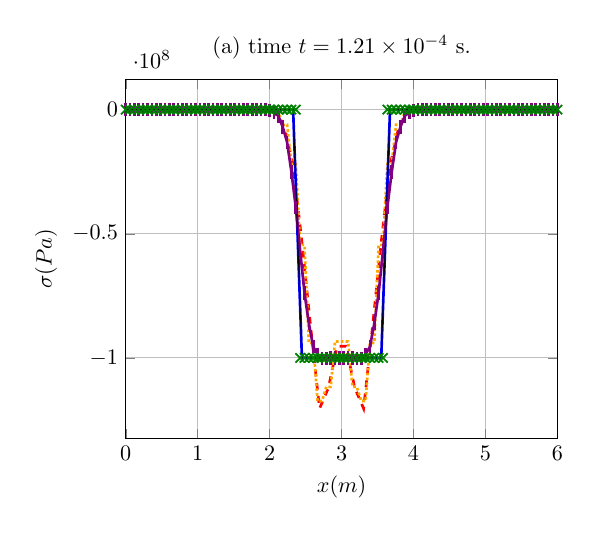
\begin{tikzpicture}[scale=0.8]
\begin{axis}[xlabel=$x (m)$,ylabel=$\sigma (Pa)$,ymajorgrids=true,xmajorgrids=true,legend pos=outer north east,title={(a) time $t = 1.21\times 10^{-4} $ s.},xmin=0.,xmax=6.]
\addplot[Red,very thick,mark=none,dashed,mark size=3pt] coordinates {(0.0,-1.7182156787438973e-08) (0.12244897959183673,4.295539196859743e-08) (0.24489795918367346,1.718215678743897e-08) (0.36734693877551017,8.591078393719486e-09) (0.4897959183673469,-1.7182156787438973e-08) (0.6122448979591837,-3.4364313574877946e-08) (0.7346938775510203,-2.5773235181158458e-08) (0.8571428571428571,0.0) (0.9795918367346939,0.0) (1.1020408163265305,-1.7182156787438973e-08) (1.2244897959183674,1.7182156787438973e-08) (1.346938775510204,0.0) (1.4693877551020407,0.0) (1.5918367346938775,0.0) (1.7142857142857142,0.0) (1.836734693877551,-10490.417480468344) (1.9591836734693877,-180244.44580078288) (2.0816326530612246,-1426887.5122070103) (2.204081632653061,-6905937.1948242355) (2.326530612244898,-22447967.529296968) (2.4489795918367347,-53339385.9863282) (2.571428571428571,-87870025.6347658) (2.693877551020408,-120363616.94335955) (2.816326530612245,-112137222.29003876) (2.9387755102040813,-95318222.04589848) (3.061224489795918,-95318222.04589835) (3.183673469387755,-112137222.29003933) (3.306122448979592,-120363616.94335933) (3.4285714285714284,-87870025.63476545) (3.5510204081632653,-53339385.98632792) (3.673469387755102,-22447967.529296756) (3.7959183673469385,-6905937.194824192) (3.9183673469387754,-1426887.512207019) (4.040816326530612,-180244.44580077427) (4.163265306122449,-10490.417480468344) (4.285714285714286,0.0) (4.408163265306122,0.0) (4.530612244897959,0.0) (4.653061224489796,0.0) (4.775510204081632,1.7182156787438973e-08) (4.8979591836734695,-1.7182156787438973e-08) (5.020408163265306,0.0) (5.142857142857142,0.0) (5.26530612244898,0.0) (5.387755102040816,0.0) (5.5102040816326525,0.0) (5.63265306122449,0.0) (5.755102040816326,0.0) (5.877551020408163,0.0) (6.0,0.0) };
\addplot[Orange,very thick,mark=none,densely dotted,mark size=3pt] coordinates {(0.0,0.0) (0.06060606060606061,0.0) (0.12121212121212122,0.0) (0.18181818181818182,0.0) (0.24242424242424243,0.0) (0.30303030303030304,0.0) (0.36363636363636365,0.0) (0.42424242424242425,0.0) (0.48484848484848486,0.0) (0.5454545454545454,0.0) (0.6060606060606061,8.504299824085957e-09) (0.6666666666666667,8.504299824085957e-09) (0.7272727272727273,-1.7008599648171914e-08) (0.7878787878787878,-1.7008599648171914e-08) (0.8484848484848485,0.0) (0.9090909090909092,0.0) (0.9696969696969697,-2.551289947225787e-08) (1.0303030303030303,-2.551289947225787e-08) (1.0909090909090908,0.0) (1.1515151515151516,0.0) (1.2121212121212122,1.7008599648171914e-08) (1.2727272727272727,1.7008599648171914e-08) (1.3333333333333335,-8.504299824085957e-09) (1.393939393939394,-8.504299824085957e-09) (1.4545454545454546,-8.504299824085957e-09) (1.5151515151515151,-8.504299824085957e-09) (1.5757575757575757,8.504299824085957e-09) (1.6363636363636365,8.504299824085957e-09) (1.696969696969697,1.7008599648171914e-08) (1.7575757575757576,1.7008599648171914e-08) (1.8181818181818183,-5499.273538584786) (1.878787878787879,-5499.273538584786) (1.9393939393939394,-115492.194890958) (2.0,-115492.194890958) (2.0606060606060606,-1086898.8931179084) (2.121212121212121,-1086898.8931179084) (2.1818181818181817,-6038592.01073648) (2.2424242424242427,-6038592.01073648) (2.303030303030303,-21882501.244545024) (2.3636363636363638,-21882501.244545024) (2.4242424242424243,-54484376.31130224) (2.484848484848485,-54484376.31130224) (2.5454545454545454,-94001361.72771455) (2.606060606060606,-94001361.72771455) (2.666666666666667,-117371180.65357204) (2.7272727272727275,-117371180.65357204) (2.787878787878788,-111648218.33372112) (2.8484848484848486,-111648218.33372112) (2.909090909090909,-93365879.35686114) (2.9696969696969697,-93365879.35686114) (3.0303030303030303,-93365879.35686119) (3.090909090909091,-93365879.35686119) (3.1515151515151514,-111648218.33372112) (3.2121212121212124,-111648218.33372112) (3.272727272727273,-117371180.6535721) (3.3333333333333335,-117371180.6535721) (3.393939393939394,-94001361.72771455) (3.4545454545454546,-94001361.72771455) (3.515151515151515,-54484376.3113022) (3.5757575757575757,-54484376.3113022) (3.6363636363636367,-21882501.24454498) (3.6969696969696972,-21882501.24454498) (3.757575757575758,-6038592.01073648) (3.8181818181818183,-6038592.01073648) (3.878787878787879,-1086898.8931178998) (3.9393939393939394,-1086898.8931178998) (4.0,-115492.19489097499) (4.0606060606060606,-115492.19489097499) (4.121212121212121,-5499.273538601796) (4.181818181818182,-5499.273538601796) (4.242424242424242,-8.504299824085957e-09) (4.303030303030303,-8.504299824085957e-09) (4.363636363636363,1.7008599648171914e-08) (4.424242424242425,1.7008599648171914e-08) (4.484848484848485,-8.504299824085957e-09) (4.545454545454546,-8.504299824085957e-09) (4.606060606060606,0.0) (4.666666666666667,0.0) (4.7272727272727275,0.0) (4.787878787878788,0.0) (4.848484848484849,0.0) (4.909090909090909,0.0) (4.96969696969697,0.0) (5.03030303030303,0.0) (5.090909090909091,0.0) (5.151515151515151,0.0) (5.212121212121212,0.0) (5.2727272727272725,0.0) (5.333333333333334,0.0) (5.3939393939393945,0.0) (5.454545454545455,0.0) (5.515151515151516,0.0) (5.575757575757576,0.0) (5.636363636363637,0.0) (5.696969696969697,0.0) (5.757575757575758,0.0) (5.818181818181818,0.0) (5.878787878787879,0.0) (5.9393939393939394,0.0) (6.0,0.0) };
\addplot[Blue,very thick,mark=none,solid,mark size=3pt] coordinates {(0.0,2.205276437763443e-23) (0.12244897959183673,-4.821391029817259e-08) (0.24489795918367346,-3.616043272362948e-08) (0.36734693877551017,2.4106955149086293e-08) (0.4897959183673469,-3.616043272362948e-08) (0.6122448979591837,-2.4106955149086323e-08) (0.7346938775510203,1.2053477574543153e-08) (0.8571428571428571,-1.205347757454316e-08) (0.9795918367346939,1.205347757454315e-08) (1.1020408163265305,1.2053477574543135e-08) (1.2244897959183674,2.4106955149086313e-08) (1.346938775510204,2.41069551490863e-08) (1.4693877551020407,-6.3007898221812655e-24) (1.5918367346938775,-6.3007898221812655e-24) (1.7142857142857142,1.2053477574543152e-08) (1.836734693877551,-2.4106955149086303e-08) (1.9591836734693877,0.0) (2.0816326530612246,0.0) (2.204081632653061,1.5751974555453164e-23) (2.326530612244898,1.5751974555453164e-23) (2.4489795918367347,-99999999.99999999) (2.571428571428571,-100000000.00000003) (2.693877551020408,-100000000.0) (2.816326530612245,-99999999.99999999) (2.9387755102040813,-100000000.0) (3.061224489795918,-99999999.99999997) (3.183673469387755,-100000000.0) (3.306122448979592,-99999999.99999999) (3.4285714285714284,-99999999.99999999) (3.5510204081632653,-99999999.99999999) (3.673469387755102,-1.2601579644362531e-23) (3.7959183673469385,1.2053477574543145e-08) (3.9183673469387754,1.2053477574543147e-08) (4.040816326530612,-3.6160432723629465e-08) (4.163265306122449,1.4176777099907847e-23) (4.285714285714286,-1.4176777099907847e-23) (4.408163265306122,-2.410695514908632e-08) (4.530612244897959,-1.2053477574543148e-08) (4.653061224489796,1.2053477574543138e-08) (4.775510204081632,-1.8902369466543796e-23) (4.8979591836734695,-1.2053477574543148e-08) (5.020408163265306,-2.4106955149086316e-08) (5.142857142857142,3.616043272362944e-08) (5.26530612244898,-1.2053477574543148e-08) (5.387755102040816,-1.8902369466543796e-23) (5.5102040816326525,2.410695514908629e-08) (5.63265306122449,-1.8902369466543796e-23) (5.755102040816326,-1.2053477574543173e-08) (5.877551020408163,2.410695514908629e-08) (6.0,-1.5751974555453164e-23) };
\addplot[Purple,very thick,mark=|,solid,mark size=3pt] coordinates {(0.0,1.1954895665669321e-11) (0.06060606060606061,-1.1954895665669323e-11) (0.12121212121212122,-9.040062200539418e-09) (0.18181818181818182,-1.5066892948546882e-08) (0.24242424242424243,-2.0148953581298875e-08) (0.30303030303030304,-4.011843429141689e-08) (0.36363636363636365,-3.9801572080816714e-08) (0.42424242424242425,-4.457277094098534e-08) (0.48484848484848486,-3.051726216575409e-08) (0.5454545454545454,-2.975012570696168e-08) (0.6060606060606061,-1.895467099939049e-08) (0.6666666666666667,-5.152284149695791e-09) (0.7272727272727273,-1.179037790916254e-08) (0.7878787878787878,-1.2316577239923773e-08) (0.8484848484848485,-2.5473583645144106e-08) (0.9090909090909092,1.3666284960577943e-09) (0.9696969696969697,3.645346560854217e-08) (1.0303030303030303,2.381392226417357e-08) (1.0909090909090908,2.4282772581015557e-08) (1.1515151515151516,2.3931137717157056e-08) (1.2121212121212122,1.2243410979431472e-08) (1.2727272727272727,1.1863544169654833e-08) (1.3333333333333335,1.2583171413268185e-08) (1.393939393939394,1.1523783735818112e-08) (1.4545454545454546,2.7371193430229355e-08) (1.5151515151515151,2.0842716867943245e-08) (1.5757575757575757,9.624966966074275e-09) (1.6363636363636365,1.448198818301203e-08) (1.696969696969697,2.104809967646104e-08) (1.7575757575757576,1.511233304716842e-08) (1.8181818181818183,-3666.244447226061) (1.878787878787879,-10998.733341690284) (1.9393939393939394,-100618.04205178331) (2.0,-262747.51871824573) (2.0606060606060606,-1140066.2362575496) (2.121212121212121,-2551162.9879474747) (2.1818181818181817,-6952185.183763518) (2.2424242424242427,-13110550.493001966) (2.303030303030303,-25132333.114743244) (2.3636363636363638,-39370855.31651974) (2.4242424242424243,-56894854.8287153) (2.484848484848485,-73865127.93600555) (2.5454545454545454,-86159824.57995412) (2.606060606060606,-95498106.62865634) (2.666666666666667,-98513982.44500154) (2.7272727272727275,-100261419.26646227) (2.787878787878788,-100094961.18873355) (2.8484848484848486,-100070640.63102004) (2.909090909090909,-100007508.13633199) (2.9696969696969697,-99998390.4883265) (3.0303030303030303,-99998390.48832652) (3.090909090909091,-100007508.136332) (3.1515151515151514,-100070640.63102002) (3.2121212121212124,-100094961.18873355) (3.272727272727273,-100261419.2664623) (3.3333333333333335,-98513982.44500159) (3.393939393939394,-95498106.62865636) (3.4545454545454546,-86159824.57995415) (3.515151515151515,-73865127.93600555) (3.5757575757575757,-56894854.8287153) (3.6363636363636367,-39370855.31651971) (3.6969696969696972,-25132333.11474323) (3.757575757575758,-13110550.493001949) (3.8181818181818183,-6952185.183763516) (3.878787878787879,-2551162.987947458) (3.9393939393939394,-1140066.2362575415) (4.0,-262747.51871824026) (4.0606060606060606,-100618.04205180079) (4.121212121212121,-10998.73334169629) (4.181818181818182,-3666.2444472321054) (4.242424242424242,6.026554865799796e-09) (4.303030303030303,6.026922708743356e-09) (4.363636363636363,2.0086063933044116e-09) (4.424242424242425,-1.4062083967847561e-08) (4.484848484848485,0.0) (4.545454545454546,0.0) (4.606060606060606,0.0) (4.666666666666667,0.0) (4.7272727272727275,0.0) (4.787878787878788,0.0) (4.848484848484849,0.0) (4.909090909090909,0.0) (4.96969696969697,0.0) (5.03030303030303,0.0) (5.090909090909091,0.0) (5.151515151515151,0.0) (5.212121212121212,0.0) (5.2727272727272725,0.0) (5.333333333333334,0.0) (5.3939393939393945,0.0) (5.454545454545455,0.0) (5.515151515151516,0.0) (5.575757575757576,0.0) (5.636363636363637,0.0) (5.696969696969697,0.0) (5.757575757575758,0.0) (5.818181818181818,0.0) (5.878787878787879,0.0) (5.9393939393939394,-6.0267272921795895e-09) (6.0,-6.026750282363563e-09) };
\addplot[Green,thick,mark=x,only marks,mark size=3pt] coordinates {(0.0,-2.1093585755450518e-08) (0.06060606060606061,-3.0133693936357875e-09) (0.12121212121212122,-2.504863308459749e-08) (0.18181818181818182,-2.316527721357512e-08) (0.24242424242424243,-1.40780851358922e-08) (0.30303030303030304,-1.0028870013194108e-08) (0.36363636363636365,-4.3717398156106705e-08) (0.42424242424242425,-2.8603467291152215e-08) (0.48484848484848486,7.156752309884969e-09) (0.5454545454545454,1.6950202839201318e-08) (0.6060606060606061,-4.3693856207718916e-08) (0.6666666666666667,-5.2733964388626276e-08) (0.7272727272727273,3.3523734504198126e-08) (0.7878787878787878,3.87971309430608e-08) (0.8484848484848485,-1.4878511381076717e-08) (0.9090909090909092,-9.228443768009598e-09) (0.9696969696969697,5.57002498854865e-08) (1.0303030303030303,8.894148100903133e-08) (1.0909090909090908,-5.925508409204129e-08) (1.1515151515151516,-3.7172736504303915e-08) (1.2121212121212122,2.895659651696907e-09) (1.2727272727272727,2.1211295497389412e-08) (1.3333333333333335,3.926796991081633e-08) (1.393939393939394,8.945940387356272e-09) (1.4545454545454546,-2.0104823923163776e-08) (1.5151515151515151,-2.810908637500884e-08) (1.5757575757575757,5.155686696923746e-09) (1.6363636363636365,-5.155686696923745e-09) (1.696969696969697,1.909252014248924e-08) (1.7575757575757576,5.014435006597071e-09) (1.8181818181818183,-1.0546792877725262e-08) (1.878787878787879,-1.3560162271361046e-08) (1.9393939393939394,-4.8967252646581575e-09) (2.0,-1.9210229884428146e-08) (2.0606060606060606,6.191532425986014e-09) (2.121212121212121,-6.191532425986031e-09) (2.1818181818181817,-1.7774171032773557e-08) (2.2424242424242427,-3.043973926539904e-08) (2.303030303030303,1.7609377394059133e-08) (2.3636363636363638,6.4975777550271785e-09) (2.4242424242424243,-99999999.99999994) (2.484848484848485,-100000000.00000006) (2.5454545454545454,-99999999.99999997) (2.606060606060606,-99999999.99999996) (2.666666666666667,-99999999.99999994) (2.7272727272727275,-99999999.99999994) (2.787878787878788,-100000000.00000001) (2.8484848484848486,-100000000.00000001) (2.909090909090909,-99999999.99999997) (2.9696969696969697,-99999999.99999999) (3.0303030303030303,-99999999.99999996) (3.090909090909091,-99999999.99999997) (3.1515151515151514,-99999999.99999996) (3.2121212121212124,-99999999.99999997) (3.272727272727273,-99999999.99999996) (3.3333333333333335,-99999999.99999999) (3.393939393939394,-99999999.99999999) (3.4545454545454546,-100000000.0) (3.515151515151515,-99999999.99999993) (3.5757575757575757,-100000000.00000009) (3.6363636363636367,0.0) (3.6969696969696972,0.0) (3.757575757575758,0.0) (3.8181818181818183,0.0) (3.878787878787879,0.0) (3.9393939393939394,0.0) (4.0,-6.026738787271577e-09) (4.0606060606060606,-1.8080216361814732e-08) (4.121212121212121,1.8080216361814716e-08) (4.181818181818182,6.0267387872715865e-09) (4.242424242424242,-1.6479363871445125e-10) (4.303030303030303,-2.3942161510371846e-08) (4.363636363636363,2.2105889536125074e-08) (4.424242424242425,2.610802076204755e-08) (4.484848484848485,-1.101763184548084e-08) (4.545454545454546,-1.308932330360547e-08) (4.606060606060606,2.4106955149086287e-08) (4.666666666666667,2.4106955149086323e-08) (4.7272727272727275,-2.4106955149086296e-08) (4.787878787878788,-2.410695514908632e-08) (4.848484848484849,0.0) (4.909090909090909,0.0) (4.96969696969697,0.0) (5.03030303030303,0.0) (5.090909090909091,0.0) (5.151515151515151,0.0) (5.212121212121212,0.0) (5.2727272727272725,0.0) (5.333333333333334,0.0) (5.3939393939393945,0.0) (5.454545454545455,0.0) (5.515151515151516,0.0) (5.575757575757576,0.0) (5.636363636363637,0.0) (5.696969696969697,0.0) (5.757575757575758,0.0) (5.818181818181818,0.0) (5.878787878787879,0.0) (5.9393939393939394,0.0) (6.0,0.0) };
\addplot[black,thin,mark=pentagone*,solid,mark size=3pt] coordinates {(0.0,-0.0) (0.12244897959183673,-0.0) (0.24489795918367346,-0.0) (0.36734693877551017,-0.0) (0.4897959183673469,-0.0) (0.6122448979591837,-0.0) (0.7346938775510203,-0.0) (0.8571428571428571,-0.0) (0.9795918367346939,-0.0) (1.1020408163265305,-0.0) (1.2244897959183674,-0.0) (1.346938775510204,-0.0) (1.4693877551020407,-0.0) (1.5918367346938775,-0.0) (1.7142857142857142,-0.0) (1.836734693877551,-0.0) (1.9591836734693877,-0.0) (2.0816326530612246,-0.0) (2.204081632653061,-0.0) (2.326530612244898,-0.0) (2.4489795918367347,-100000000.0) (2.571428571428571,-100000000.0) (2.693877551020408,-100000000.0) (2.816326530612245,-100000000.0) (2.9387755102040813,-100000000.0) (3.061224489795918,-100000000.0) (3.183673469387755,-100000000.0) (3.306122448979592,-100000000.0) (3.4285714285714284,-100000000.0) (3.5510204081632653,-100000000.0) (3.673469387755102,-0.0) (3.7959183673469385,-0.0) (3.9183673469387754,-0.0) (4.040816326530612,-0.0) (4.163265306122449,-0.0) (4.285714285714286,-0.0) (4.408163265306122,-0.0) (4.530612244897959,-0.0) (4.653061224489796,-0.0) (4.775510204081632,-0.0) (4.8979591836734695,-0.0) (5.020408163265306,-0.0) (5.142857142857142,-0.0) (5.26530612244898,-0.0) (5.387755102040816,-0.0) (5.5102040816326525,-0.0) (5.63265306122449,-0.0) (5.755102040816326,-0.0) (5.877551020408163,-0.0) (6.0,-0.0) };
%\legend{usl 1ppc,usl 2ppc,dgmpm 1ppc,dgmpm 2ppc,dgmpm 2ppc (RK2),exact}
\end{axis}
\end{tikzpicture}
%%% Local Variables:
%%% mode: latex
%%% TeX-master: "../../mainManuscript"
%%% End:
}
  {\begin{tikzpicture}[scale=0.9]
\begin{axis}[xlabel=$x (m)$,ylabel=$\sigma (Pa)$,ymajorgrids=true,xmajorgrids=true,legend pos=outer north east,title={(b) time $t = 4.84\times 10^{-4} $ s.},xmin=0.,xmax=6.]
\addplot[Red,very thick,mark=none,dashed,mark size=3pt] coordinates {(0.0,-745947.6317356245) (0.12244897959183673,-2825505.704681147) (0.24489795918367346,-6801870.379054734) (0.36734693877551017,-14249320.469123462) (0.4897959183673469,-26743878.38137685) (0.6122448979591837,-45064188.07482756) (0.7346938775510203,-68064481.52123177) (0.8571428571428571,-91948308.59367745) (0.9795918367346939,-110948018.79598898) (1.1020408163265305,-119819288.51732583) (1.2244897959183674,-117150564.11810811) (1.346938775510204,-106891678.01826178) (1.4693877551020407,-96652794.70257169) (1.5918367346938775,-92267743.75879696) (1.7142857142857142,-95070577.34692116) (1.836734693877551,-99847820.1972167) (1.9591836734693877,-103232485.94759263) (2.0816326530612246,-101626491.39890483) (2.204081632653061,-100355242.65368447) (2.326530612244898,-98244216.75952996) (2.4489795918367347,-100067772.41751443) (2.571428571428571,-99702418.44172558) (2.693877551020408,-100893884.04862353) (2.816326530612245,-99751345.3825965) (2.9387755102040813,-99889896.90888087) (3.061224489795918,-99889896.90888077) (3.183673469387755,-99751345.38259669) (3.306122448979592,-100893884.04862344) (3.4285714285714284,-99702418.44172575) (3.5510204081632653,-100067772.41751438) (3.673469387755102,-98244216.75953004) (3.7959183673469385,-100355242.65368438) (3.9183673469387754,-101626491.39890482) (4.040816326530612,-103232485.94759259) (4.163265306122449,-99847820.1972167) (4.285714285714286,-95070577.34692109) (4.408163265306122,-92267743.7587969) (4.530612244897959,-96652794.70257166) (4.653061224489796,-106891678.01826191) (4.775510204081632,-117150564.11810826) (4.8979591836734695,-119819288.51732588) (5.020408163265306,-110948018.79598887) (5.142857142857142,-91948308.59367728) (5.26530612244898,-68064481.52123177) (5.387755102040816,-45064188.074827455) (5.5102040816326525,-26743878.38137681) (5.63265306122449,-14249320.469123438) (5.755102040816326,-6801870.379054725) (5.877551020408163,-2825505.7046811893) (6.0,-745947.6317356417) };
\addplot[Duck,thin,mark=*,solid,mark size=3pt] coordinates {(0.0,-3658473.820541984) (0.12244897959183673,-11485497.138528435) (0.24489795918367346,-20650075.223420583) (0.36734693877551017,-31470071.326657515) (0.4897959183673469,-43620393.930359595) (0.6122448979591837,-56234556.96822935) (0.7346938775510203,-68199491.57707022) (0.8571428571428571,-78518360.75669788) (0.9795918367346939,-86590219.21803293) (1.1020408163265305,-92306933.66125712) (1.2244897959183674,-95965467.32727806) (1.346938775510204,-98076133.61253974) (1.4693877551020407,-99170549.7565818) (1.5918367346938775,-99678671.19148654) (1.7142857142857142,-99888928.31124762) (1.836734693877551,-99966022.58725037) (1.9591836734693877,-99990891.70851223) (2.0816326530612246,-99997886.14886712) (2.204081632653061,-99999581.77077132) (2.326530612244898,-99999930.86939865) (2.4489795918367347,-99999990.71487762) (2.571428571428571,-99999999.0267497) (2.693877551020408,-99999999.92533047) (2.816326530612245,-99999999.99627104) (2.9387755102040813,-99999999.99990901) (3.061224489795918,-99999999.99990901) (3.183673469387755,-99999999.99627106) (3.306122448979592,-99999999.9253305) (3.4285714285714284,-99999999.02674973) (3.5510204081632653,-99999990.71487764) (3.673469387755102,-99999930.86939867) (3.7959183673469385,-99999581.77077134) (3.9183673469387754,-99997886.14886712) (4.040816326530612,-99990891.70851222) (4.163265306122449,-99966022.58725034) (4.285714285714286,-99888928.31124759) (4.408163265306122,-99678671.19148651) (4.530612244897959,-99170549.75658175) (4.653061224489796,-98076133.61253972) (4.775510204081632,-95965467.32727805) (4.8979591836734695,-92306933.66125712) (5.020408163265306,-86590219.21803287) (5.142857142857142,-78518360.7566978) (5.26530612244898,-68199491.5770702) (5.387755102040816,-56234556.968229264) (5.5102040816326525,-43620393.930359535) (5.63265306122449,-31470071.32665747) (5.755102040816326,-20650075.223420557) (5.877551020408163,-11485497.138528453) (6.0,-3658473.8205419495) };
\addplot[Orange,very thick,mark=none,densely dotted,mark size=3pt] coordinates {(0.0,-569245.6271305095) (0.06060606060606061,-569245.6271305095) (0.12121212121212122,-2277785.4230159773) (0.18181818181818182,-2277785.4230159773) (0.24242424242424243,-5901161.70250096) (0.30303030303030304,-5901161.70250096) (0.36363636363636365,-13233001.909618562) (0.42424242424242425,-13233001.909618562) (0.48484848484848486,-26238300.23104623) (0.5454545454545454,-26238300.23104623) (0.6060606060606061,-45981632.22002476) (0.6666666666666667,-45981632.22002476) (0.7272727272727273,-70997511.41827326) (0.7878787878787878,-70997511.41827326) (0.8484848484848485,-96258666.79270092) (0.9090909090909092,-96258666.79270092) (0.9696969696969697,-114407544.96327573) (1.0303030303030303,-114407544.96327573) (1.0909090909090908,-119769201.2337222) (1.1515151515151516,-119769201.2337222) (1.2121212121212122,-112838974.87666531) (1.2727272727272727,-112838974.87666531) (1.3333333333333335,-100993168.67842056) (1.393939393939394,-100993168.67842056) (1.4545454545454546,-93414330.53328812) (1.5151515151515151,-93414330.53328812) (1.5757575757575757,-93992004.01740366) (1.6363636363636365,-93992004.01740366) (1.696969696969697,-99087098.74325639) (1.7575757575757576,-99087098.74325639) (1.8181818181818183,-102489655.2966868) (1.878787878787879,-102489655.2966868) (1.9393939393939394,-101890791.3937958) (2.0,-101890791.3937958) (2.0606060606060606,-99782074.12880751) (2.121212121212121,-99782074.12880751) (2.1818181818181817,-99055570.19076754) (2.2424242424242427,-99055570.19076754) (2.303030303030303,-99748095.76886229) (2.3636363636363638,-99748095.76886229) (2.4242424242424243,-100313223.73164806) (2.484848484848485,-100313223.73164806) (2.5454545454545454,-100175907.04998955) (2.606060606060606,-100175907.04998955) (2.666666666666667,-99908114.85126807) (2.7272727272727275,-99908114.85126807) (2.787878787878788,-99919571.77694954) (2.8484848484848486,-99919571.77694954) (2.909090909090909,-100047873.551725) (2.9696969696969697,-100047873.551725) (3.0303030303030303,-100047873.55172497) (3.090909090909091,-100047873.55172497) (3.1515151515151514,-99919571.7769495) (3.2121212121212124,-99919571.7769495) (3.272727272727273,-99908114.851268) (3.3333333333333335,-99908114.851268) (3.393939393939394,-100175907.0499895) (3.4545454545454546,-100175907.0499895) (3.515151515151515,-100313223.73164806) (3.5757575757575757,-100313223.73164806) (3.6363636363636367,-99748095.7688623) (3.6969696969696972,-99748095.7688623) (3.757575757575758,-99055570.19076759) (3.8181818181818183,-99055570.19076759) (3.878787878787879,-99782074.12880753) (3.9393939393939394,-99782074.12880753) (4.0,-101890791.39379583) (4.0606060606060606,-101890791.39379583) (4.121212121212121,-102489655.29668684) (4.181818181818182,-102489655.29668684) (4.242424242424242,-99087098.74325638) (4.303030303030303,-99087098.74325638) (4.363636363636363,-93992004.01740365) (4.424242424242425,-93992004.01740365) (4.484848484848485,-93414330.53328809) (4.545454545454546,-93414330.53328809) (4.606060606060606,-100993168.67842054) (4.666666666666667,-100993168.67842054) (4.7272727272727275,-112838974.87666531) (4.787878787878788,-112838974.87666531) (4.848484848484849,-119769201.2337222) (4.909090909090909,-119769201.2337222) (4.96969696969697,-114407544.96327575) (5.03030303030303,-114407544.96327575) (5.090909090909091,-96258666.79270092) (5.151515151515151,-96258666.79270092) (5.212121212121212,-70997511.41827326) (5.2727272727272725,-70997511.41827326) (5.333333333333334,-45981632.22002478) (5.3939393939393945,-45981632.22002478) (5.454545454545455,-26238300.23104622) (5.515151515151516,-26238300.23104622) (5.575757575757576,-13233001.90961853) (5.636363636363637,-13233001.90961853) (5.696969696969697,-5901161.702500943) (5.757575757575758,-5901161.702500943) (5.818181818181818,-2277785.4230159433) (5.878787878787879,-2277785.4230159433) (5.9393939393939394,-569245.627130518) (6.0,-569245.627130518) };
\addplot[Blue,very thick,mark=none,solid,mark size=3pt] coordinates {(0.0,6.026738787271584e-08) (0.12244897959183673,-1.2053477574543037e-08) (0.24489795918367346,2.410695514908625e-08) (0.36734693877551017,2.4106955149086283e-08) (0.4897959183673469,6.026738787271564e-08) (0.6122448979591837,-99999999.99999984) (0.7346938775510203,-100000000.00000025) (0.8571428571428571,-99999999.9999998) (0.9795918367346939,-100000000.00000009) (1.1020408163265305,-99999999.99999985) (1.2244897959183674,-100000000.0) (1.346938775510204,-99999999.99999991) (1.4693877551020407,-100000000.0) (1.5918367346938775,-99999999.99999979) (1.7142857142857142,-100000000.00000003) (1.836734693877551,-99999999.99999988) (1.9591836734693877,-99999999.99999994) (2.0816326530612246,-99999999.99999994) (2.204081632653061,-99999999.99999999) (2.326530612244898,-99999999.99999991) (2.4489795918367347,-99999999.99999991) (2.571428571428571,-99999999.99999997) (2.693877551020408,-99999999.99999991) (2.816326530612245,-99999999.99999994) (2.9387755102040813,-99999999.99999997) (3.061224489795918,-99999999.99999988) (3.183673469387755,-99999999.99999997) (3.306122448979592,-99999999.99999988) (3.4285714285714284,-100000000.00000003) (3.5510204081632653,-99999999.99999991) (3.673469387755102,-100000000.0) (3.7959183673469385,-100000000.00000003) (3.9183673469387754,-99999999.99999987) (4.040816326530612,-99999999.99999997) (4.163265306122449,-99999999.99999994) (4.285714285714286,-99999999.99999997) (4.408163265306122,-99999999.99999997) (4.530612244897959,-100000000.00000009) (4.653061224489796,-99999999.99999988) (4.775510204081632,-100000000.00000013) (4.8979591836734695,-99999999.99999987) (5.020408163265306,-100000000.00000012) (5.142857142857142,-99999999.99999991) (5.26530612244898,-100000000.00000007) (5.387755102040816,-99999999.99999999) (5.5102040816326525,-2.410695514908632e-08) (5.63265306122449,2.410695514908628e-08) (5.755102040816326,-7.232086544725893e-08) (5.877551020408163,-1.205347757454315e-08) (6.0,-2.4106955149086326e-08) };
\addplot[Purple,very thick,mark=|,solid,mark size=3pt] coordinates {(0.0,-901250.8727450209) (0.06060606060606061,-2481132.001666541) (0.12121212121212122,-4826425.776536643) (0.18181818181818182,-7379655.632326556) (0.24242424242424243,-11256070.988140773) (0.30303030303030304,-15619284.087205578) (0.36363636363636365,-21632650.461414523) (0.42424242424242425,-28194347.738026302) (0.48484848484848486,-36184793.045001954) (0.5454545454545454,-44512745.90296996) (0.6060606060606061,-53388027.81990887) (0.6666666666666667,-62184684.90343942) (0.7272727272727273,-70312839.86926234) (0.7878787878787878,-77956322.11918701) (0.8484848484848485,-83999795.65014975) (0.9090909090909092,-89383013.54381928) (0.9696969696969697,-92952697.00923085) (1.0303030303030303,-95962268.87367085) (1.0909090909090908,-97581224.04592441) (1.1515151515151516,-98874662.75556055) (1.2121212121212122,-99404486.29729274) (1.2727272727272727,-99808341.57283215) (1.3333333333333335,-99915762.38856114) (1.393939393939394,-99996248.63365263) (1.4545454545454546,-100001427.378495) (1.5151515151515151,-100006998.37736051) (1.5757575757575757,-100003237.88768458) (1.6363636363636365,-100001492.41546689) (1.696969696969697,-100000520.10664989) (1.7575757575757576,-100000028.36063254) (1.8181818181818183,-99999995.05295742) (1.878787878787879,-99999970.09524688) (1.9393939393939394,-99999990.32856694) (2.0,-99999997.18169779) (2.0606060606060606,-99999999.42352416) (2.121212121212121,-100000000.25132437) (2.1818181818181817,-100000000.07258461) (2.2424242424242427,-100000000.03564933) (2.303030303030303,-100000000.00601049) (2.3636363636363638,-99999999.99877489) (2.4242424242424243,-99999999.99971391) (2.484848484848485,-99999999.99982226) (2.5454545454545454,-99999999.99998015) (2.606060606060606,-100000000.00000417) (2.666666666666667,-100000000.00000048) (2.7272727272727275,-100000000.0000002) (2.787878787878788,-99999999.99999994) (2.8484848484848486,-99999999.99999994) (2.909090909090909,-99999999.99999994) (2.9696969696969697,-99999999.99999994) (3.0303030303030303,-99999999.99999994) (3.090909090909091,-99999999.99999994) (3.1515151515151514,-99999999.99999996) (3.2121212121212124,-99999999.99999997) (3.272727272727273,-100000000.00000024) (3.3333333333333335,-100000000.00000054) (3.393939393939394,-100000000.0000042) (3.4545454545454546,-99999999.99998017) (3.515151515151515,-99999999.99982227) (3.5757575757575757,-99999999.99971391) (3.6363636363636367,-99999999.99877487) (3.6969696969696972,-100000000.00601052) (3.757575757575758,-100000000.03564937) (3.8181818181818183,-100000000.07258466) (3.878787878787879,-100000000.2513244) (3.9393939393939394,-99999999.42352419) (4.0,-99999997.18169783) (4.0606060606060606,-99999990.328567) (4.121212121212121,-99999970.09524693) (4.181818181818182,-99999995.05295746) (4.242424242424242,-100000028.36063258) (4.303030303030303,-100000520.10664994) (4.363636363636363,-100001492.41546696) (4.424242424242425,-100003237.88768464) (4.484848484848485,-100006998.37736058) (4.545454545454546,-100001427.37849504) (4.606060606060606,-99996248.63365267) (4.666666666666667,-99915762.38856122) (4.7272727272727275,-99808341.57283223) (4.787878787878788,-99404486.29729284) (4.848484848484849,-98874662.75556065) (4.909090909090909,-97581224.04592451) (4.96969696969697,-95962268.87367095) (5.03030303030303,-92952697.00923099) (5.090909090909091,-89383013.5438194) (5.151515151515151,-83999795.65014987) (5.212121212121212,-77956322.11918712) (5.2727272727272725,-70312839.86926243) (5.333333333333334,-62184684.90343948) (5.3939393939393945,-53388027.81990896) (5.454545454545455,-44512745.90297001) (5.515151515151516,-36184793.04500202) (5.575757575757576,-28194347.73802632) (5.636363636363637,-21632650.461414546) (5.696969696969697,-15619284.087205617) (5.757575757575758,-11256070.988140827) (5.818181818181818,-7379655.632326601) (5.878787878787879,-4826425.7765366705) (5.9393939393939394,-2481132.001666579) (6.0,-901250.8727450437) };
\addplot[Green,thick,mark=x,only marks,mark size=3pt] coordinates {(0.0,-6.52473551238276e-08) (0.06060606060606061,-5.528742062160391e-08) (0.12121212121212122,-5.4360491549496524e-08) (0.18181818181818182,-4.206732904684871e-08) (0.24242424242424243,2.6389399231237735e-10) (0.30303030303030304,2.3843061156773917e-08) (0.36363636363636365,1.6444762021031894e-08) (0.42424242424242425,7.662193128054401e-09) (0.48484848484848486,-2.6065356036709213e-08) (0.5454545454545454,-4.625550941054968e-08) (0.6060606060606061,-99999999.99999985) (0.6666666666666667,-99999999.99999993) (0.7272727272727273,-99999999.99999994) (0.7878787878787878,-99999999.99999994) (0.8484848484848485,-99999999.99999994) (0.9090909090909092,-99999999.99999994) (0.9696969696969697,-100000000.0) (1.0303030303030303,-100000000.0) (1.0909090909090908,-99999999.99999988) (1.1515151515151516,-99999999.9999999) (1.2121212121212122,-99999999.99999991) (1.2727272727272727,-99999999.99999993) (1.3333333333333335,-99999999.99999996) (1.393939393939394,-99999999.99999997) (1.4545454545454546,-99999999.99999988) (1.5151515151515151,-99999999.99999988) (1.5757575757575757,-99999999.99999991) (1.6363636363636365,-99999999.99999993) (1.696969696969697,-99999999.99999997) (1.7575757575757576,-99999999.99999999) (1.8181818181818183,-99999999.99999994) (1.878787878787879,-99999999.99999994) (1.9393939393939394,-99999999.99999994) (2.0,-99999999.99999994) (2.0606060606060606,-99999999.99999996) (2.121212121212121,-99999999.99999999) (2.1818181818181817,-99999999.99999996) (2.2424242424242427,-99999999.99999997) (2.303030303030303,-99999999.99999994) (2.3636363636363638,-99999999.99999994) (2.4242424242424243,-99999999.99999994) (2.484848484848485,-99999999.99999994) (2.5454545454545454,-99999999.9999999) (2.606060606060606,-99999999.99999993) (2.666666666666667,-99999999.99999994) (2.7272727272727275,-99999999.99999994) (2.787878787878788,-99999999.99999996) (2.8484848484848486,-99999999.99999999) (2.909090909090909,-99999999.99999991) (2.9696969696969697,-99999999.99999993) (3.0303030303030303,-99999999.99999994) (3.090909090909091,-99999999.99999994) (3.1515151515151514,-99999999.99999994) (3.2121212121212124,-99999999.99999994) (3.272727272727273,-100000000.0) (3.3333333333333335,-100000000.0) (3.393939393939394,-99999999.99999991) (3.4545454545454546,-99999999.99999993) (3.515151515151515,-99999999.99999999) (3.5757575757575757,-100000000.0) (3.6363636363636367,-99999999.99999991) (3.6969696969696972,-99999999.99999993) (3.757575757575758,-99999999.99999993) (3.8181818181818183,-99999999.99999994) (3.878787878787879,-100000000.00000004) (3.9393939393939394,-100000000.00000003) (4.0,-99999999.99999991) (4.0606060606060606,-99999999.99999991) (4.121212121212121,-100000000.00000001) (4.181818181818182,-100000000.00000003) (4.242424242424242,-99999999.99999993) (4.303030303030303,-99999999.99999994) (4.363636363636363,-99999999.99999997) (4.424242424242425,-99999999.99999997) (4.484848484848485,-100000000.00000006) (4.545454545454546,-100000000.00000006) (4.606060606060606,-99999999.99999991) (4.666666666666667,-99999999.99999993) (4.7272727272727275,-99999999.99999996) (4.787878787878788,-99999999.99999997) (4.848484848484849,-99999999.99999996) (4.909090909090909,-99999999.99999999) (4.96969696969697,-99999999.99999997) (5.03030303030303,-99999999.99999996) (5.090909090909091,-99999999.99999997) (5.151515151515151,-99999999.99999999) (5.212121212121212,-99999999.99999996) (5.2727272727272725,-99999999.99999997) (5.333333333333334,-99999999.99999991) (5.3939393939393945,-100000000.00000009) (5.454545454545455,-6.171875818689624e-09) (5.515151515151516,6.171875818689572e-09) (5.575757575757576,-3.413288241873195e-08) (5.636363636363637,-6.229493817761331e-08) (5.696969696969697,2.564453865316311e-08) (5.757575757575758,-1.5375835040768292e-09) (5.818181818181818,-5.420092204753976e-08) (5.878787878787879,-4.222689854880543e-08) (5.9393939393939394,3.843223074305013e-09) (6.0,-3.8432230743049925e-09) };
\addplot[black,thin,mark=none,solid,mark size=3pt] coordinates {(0.0,-0.0) (0.12244897959183673,-0.0) (0.24489795918367346,-0.0) (0.36734693877551017,-0.0) (0.4897959183673469,-0.0) (0.6122448979591837,-100000000.0) (0.7346938775510203,-100000000.0) (0.8571428571428571,-100000000.0) (0.9795918367346939,-100000000.0) (1.1020408163265305,-100000000.0) (1.2244897959183674,-100000000.0) (1.346938775510204,-100000000.0) (1.4693877551020407,-100000000.0) (1.5918367346938775,-100000000.0) (1.7142857142857142,-100000000.0) (1.836734693877551,-100000000.0) (1.9591836734693877,-100000000.0) (2.0816326530612246,-100000000.0) (2.204081632653061,-100000000.0) (2.326530612244898,-100000000.0) (2.4489795918367347,-100000000.0) (2.571428571428571,-100000000.0) (2.693877551020408,-100000000.0) (2.816326530612245,-100000000.0) (2.9387755102040813,-100000000.0) (3.061224489795918,-100000000.0) (3.183673469387755,-100000000.0) (3.306122448979592,-100000000.0) (3.4285714285714284,-100000000.0) (3.5510204081632653,-100000000.0) (3.673469387755102,-100000000.0) (3.7959183673469385,-100000000.0) (3.9183673469387754,-100000000.0) (4.040816326530612,-100000000.0) (4.163265306122449,-100000000.0) (4.285714285714286,-100000000.0) (4.408163265306122,-100000000.0) (4.530612244897959,-100000000.0) (4.653061224489796,-100000000.0) (4.775510204081632,-100000000.0) (4.8979591836734695,-100000000.0) (5.020408163265306,-100000000.0) (5.142857142857142,-100000000.0) (5.26530612244898,-100000000.0) (5.387755102040816,-100000000.0) (5.5102040816326525,-0.0) (5.63265306122449,-0.0) (5.755102040816326,-0.0) (5.877551020408163,-0.0) (6.0,-0.0) };
%\legend{usl 1ppc,usl-pic 1ppc,usl 2ppc,dgmpm 1ppc,dgmpm 2ppc,dgmpm 2ppc (RK2),exact}
\end{axis}
\end{tikzpicture}
%%% Local Variables:
%%% mode: latex
%%% TeX-master: "../../mainManuscript"
%%% End:
}
  {\begin{tikzpicture}[scale=.675]
\begin{axis}[xlabel=$time \: (s)$,ylabel=$\frac{e}{e_{max}}$,ymajorgrids=true,xmajorgrids=true,legend pos=outer north east,title={Energy plots}]
\addplot[Red,very thick,mark=none,dashed,mark size=2pt] coordinates {(0.0,0.987654320988) (1.2090867954e-05,0.997530864198) (2.41817359079e-05,1.0) (3.62726038619e-05,0.995910493827) (4.83634718158e-05,0.98940007716) (6.04543397698e-05,0.984093484761) (7.25452077237e-05,0.981362538279) (8.46360756777e-05,0.980572573344) (9.67269436317e-05,0.980353499636) (0.000108817811586,0.979737335844) (0.00012090867954,0.97855223305) (0.000132999547494,0.977156270039) (0.000145090415447,0.975958347691) (0.000157181283401,0.97511659562) (0.000169272151355,0.974530084065) (0.000181363019309,0.974005554053) (0.000193453887263,0.97341779498) (0.000205544755217,0.972760977912) (0.000217635623171,0.972101158286) (0.000229726491125,0.971500815494) (0.000241817359079,0.970976328432) (0.000253908227033,0.970503354023) (0.000265999094987,0.970047511625) (0.000278089962941,0.969589945626) (0.000290180830895,0.969132703566) (0.000302271698849,0.968688192138) (0.000314362566803,0.96826592316) (0.000326453434757,0.967866441189) (0.000338544302711,0.96748370195) (0.000350635170665,0.967111035083) (0.000362726038619,0.96674530374) (0.000374816906573,0.9663871534) (0.000386907774527,0.96603867283) (0.000398998642481,0.965701020803) (0.000411089510435,0.9653736209) (0.000423180378389,0.965054863002) (0.000435271246342,0.96474325827) (0.000447362114296,0.964438078134) (0.00045945298225,0.964139187671) (0.000471543850204,0.963846345834) (0.000483634718158,0.963558300848) (0.000495725586112,0.963271635613) (0.000507816454066,0.962978858237) (0.00051990732202,0.962665035247) (0.000531998189974,0.962302555824) (0.000544089057928,0.961844496637) (0.000556179925882,0.961218491107) (0.000568270793836,0.960324692645) (0.00058036166179,0.959042628999) (0.000592452529744,0.95725134199) };
\addplot[Orange,very thick,mark=none,densely dotted,mark size=3pt] coordinates {(0.0,0.987349583462) (1.19687379746e-05,0.997223079297) (2.39374759493e-05,1.0) (3.59062139239e-05,0.996543312249) (4.78749518985e-05,0.991672401699) (5.98436898731e-05,0.988645826067) (7.18124278478e-05,0.98773805255) (8.37811658224e-05,0.987631618227) (9.5749903797e-05,0.987207209533) (0.000107718641772,0.98625862112) (0.000119687379746,0.985162495947) (0.000131656117721,0.984278008796) (0.000143624855696,0.983664883566) (0.00015559359367,0.983176360212) (0.000167562331645,0.982669899583) (0.000179531069619,0.982113551237) (0.000191499807594,0.981554758898) (0.000203468545569,0.981041934115) (0.000215437283543,0.980583060318) (0.000227406021518,0.98015640132) (0.000239374759493,0.979740132791) (0.000251343497467,0.97932838866) (0.000263312235442,0.978927266369) (0.000275280973416,0.978543296202) (0.000287249711391,0.978177057907) (0.000299218449366,0.977824634311) (0.00031118718734,0.977482093196) (0.000323155925315,0.977147995987) (0.00033512466329,0.976822820567) (0.000347093401264,0.976507170495) (0.000359062139239,0.976200756538) (0.000371030877213,0.975902607469) (0.000382999615188,0.97561177268) (0.000394968353163,0.97532772239) (0.000406937091137,0.975050257459) (0.000418905829112,0.974779220922) (0.000430874567087,0.97451432881) (0.000442843305061,0.974255192075) (0.000454812043036,0.974001394871) (0.00046678078101,0.973752448152) (0.000478749518985,0.973507455428) (0.00049071825696,0.973264255861) (0.000502686994934,0.973017591891) (0.000514655732909,0.972755592972) (0.000526624470884,0.972453855054) (0.000538593208858,0.972067038786) (0.000550561946833,0.971519585751) (0.000562530684807,0.970699836135) (0.000574499422782,0.969464605892) (0.000586468160757,0.967662115176) };
\addplot[Duck,thick,mark=*,solid,mark size=2pt] coordinates {(0.0,1.0) (1.19687379746e-05,0.9825) (2.39374759493e-05,0.97517578125) (3.59062139239e-05,0.969031906128) (4.78749518985e-05,0.96380058825) (5.98436898731e-05,0.959171754479) (7.18124278478e-05,0.954982516842) (8.37811658224e-05,0.951129379832) (9.5749903797e-05,0.947543340455) (0.000107718641772,0.944175962079) (0.000119687379746,0.940991760326) (0.000131656117721,0.93796387047) (0.000143624855696,0.935071387013) (0.00015559359367,0.932297671085) (0.000167562331645,0.929629226561) (0.000179531069619,0.927054929147) (0.000191499807594,0.924565482142) (0.000203468545569,0.922153022591) (0.000215437283543,0.91981083008) (0.000227406021518,0.917533107309) (0.000239374759493,0.91531481198) (0.000251343497467,0.913151526055) (0.000263312235442,0.911039352738) (0.000275280973416,0.908974834313) (0.000287249711391,0.906954885898) (0.000299218449366,0.904976741526) (0.00031118718734,0.903037909836) (0.000323155925315,0.901136137378) (0.00033512466329,0.89926937799) (0.000347093401264,0.897435767059) (0.000359062139239,0.895633599746) (0.000371030877213,0.893861312443) (0.000382999615188,0.892117466744) (0.000394968353163,0.890400734736) (0.000406937091137,0.888709882017) (0.000418905829112,0.88704373739) (0.000430874567087,0.88540112132) (0.000442843305061,0.883780678009) (0.000454812043036,0.882180531538) (0.00046678078101,0.880597698856) (0.000478749518985,0.879027284148) (0.00049071825696,0.877461660668) (0.000502686994934,0.875890051367) (0.000514655732909,0.874299006831) (0.000526624470884,0.87267411056) (0.000538593208858,0.871002801233) (0.000550561946833,0.869277656037) (0.000562530684807,0.867499110287) (0.000574499422782,0.865676626234) (0.000586468160757,0.86382779387) };
\addplot[Blue,very thick,mark=none,solid,mark size=3pt] coordinates {(0.0,1.0) (2.41817359079e-05,1.0) (4.83634718158e-05,1.0) (7.25452077237e-05,1.0) (9.67269436317e-05,1.0) (0.00012090867954,1.0) (0.000145090415447,1.0) (0.000169272151355,1.0) (0.000193453887263,1.0) (0.000217635623171,1.0) (0.000241817359079,1.0) (0.000265999094987,1.0) (0.000290180830895,1.0) (0.000314362566803,1.0) (0.000338544302711,1.0) (0.000362726038619,1.0) (0.000386907774527,1.0) (0.000411089510435,1.0) (0.000435271246342,1.0) (0.00045945298225,1.0) (0.000483634718158,1.0) (0.000507816454066,1.0) (0.000531998189974,1.0) (0.000556179925882,1.0) (0.00058036166179,1.0) (0.000604543397698,1.0) };
\addplot[Purple,very thick,mark=+,solid,mark size=3pt] coordinates {(0.0,1.0) (1.19687379746e-05,0.985) (2.39374759493e-05,0.97828125) (3.59062139239e-05,0.972868652344) (4.78749518985e-05,0.968517532349) (5.98436898731e-05,0.964676422477) (7.18124278478e-05,0.961224535313) (8.37811658224e-05,0.95805841396) (9.5749903797e-05,0.955117021818) (0.000107718641772,0.952358340029) (0.000119687379746,0.949751847063) (0.000131656117721,0.947274776455) (0.000143624855696,0.944909512757) (0.00015559359367,0.942642119513) (0.000167562331645,0.940461338934) (0.000179531069619,0.938357922299) (0.000191499807594,0.936324160701) (0.000203468545569,0.934353548006) (0.000215437283543,0.932440533241) (0.000227406021518,0.93058033492) (0.000239374759493,0.928768799379) (0.000251343497467,0.927002291004) (0.000263312235442,0.925277605976) (0.000275280973416,0.923591903662) (0.000287249711391,0.921942651418) (0.000299218449366,0.920327579747) (0.00031118718734,0.918744645509) (0.000323155925315,0.917192001508) (0.00033512466329,0.915667971129) (0.000347093401264,0.91417102706) (0.000359062139239,0.9126997733) (0.000371030877213,0.911252929874) (0.000382999615188,0.909829319753) (0.000394968353163,0.908427857623) (0.000406937091137,0.907047540169) (0.000418905829112,0.905687437658) (0.000430874567087,0.904346686589) (0.000442843305061,0.903024483275) (0.000454812043036,0.901720078186) (0.00046678078101,0.900432770981) (0.000478749518985,0.899161906097) (0.00049071825696,0.897906868838) (0.000502686994934,0.896667081898) (0.000514655732909,0.895442002248) (0.000526624470884,0.894231118352) (0.000538593208858,0.89303394767) (0.000550561946833,0.891850034402) (0.000562530684807,0.890678947462) (0.000574499422782,0.889520278638) (0.000586468160757,0.888373640933) (0.000598436898731,0.887238667044) };
\addplot[Green,thick,mark=x,only marks,mark size=3pt] coordinates {(0.0,1.0) (2.39374759493e-05,1.0) (4.78749518985e-05,1.0) (7.18124278478e-05,1.0) (9.5749903797e-05,1.0) (0.000119687379746,1.0) (0.000143624855696,1.0) (0.000167562331645,1.0) (0.000191499807594,1.0) (0.000215437283543,1.0) (0.000239374759493,1.0) (0.000263312235442,1.0) (0.000287249711391,1.0) (0.00031118718734,1.0) (0.00033512466329,1.0) (0.000359062139239,1.0) (0.000382999615188,1.0) (0.000406937091137,1.0) (0.000430874567087,1.0) (0.000454812043036,1.0) (0.000478749518985,1.0) (0.000502686994934,1.0) (0.000526624470884,1.0) (0.000550561946833,1.0) (0.000574499422782,1.0) (0.000598436898731,1.0) };
\legend{mpm-flip 1ppc -- CFL=0.5,mpm-flip 2ppc -- CFL=0.5,mpm-pic 2ppc -- CFL=0.5,dgmpm 1ppc -- CFL=1,dgmpm 2ppc -- CFL=0.5,dgmpm 2ppc (RK2) -- CFL=1}
\end{axis}
\end{tikzpicture}
%%% Local Variables:
%%% mode: latex
%%% TeX-master: "../../presentation"
%%% End:
}
  \caption{elastic RP stress and energies}
  \label{fig:stress_elastic_RP}
\end{figure}
\begin{figure}[h!]
  \centering
  {\begin{tikzpicture}[scale=0.9]
\begin{axis}[xlabel=$x (m)$,ylabel=$v (m/s)$,ymajorgrids=true,xmajorgrids=true,legend pos=south west,title={(a) time $t = 1.21\times 10^{-4} $ s.},xmin=0.,xmax=6.]
\addplot[Red,very thick,mark=none,dashed,mark size=3pt] coordinates {(0.0,2.5318484177091665) (0.12244897959183673,2.5318484177091665) (0.24489795918367346,2.531848417709166) (0.36734693877551017,2.531848417709166) (0.4897959183673469,2.5318484177091656) (0.6122448979591837,2.5318484177091665) (0.7346938775510203,2.531848417709167) (0.8571428571428571,2.5318484177091665) (0.9795918367346939,2.5318484177091665) (1.1020408163265305,2.5318484177091665) (1.2244897959183674,2.5318484177091665) (1.346938775510204,2.5318484177091665) (1.4693877551020407,2.5318484177091665) (1.5918367346938775,2.5318484177091665) (1.7142857142857142,2.5318484177091665) (1.836734693877551,2.531684227710154) (1.9591836734693877,2.528883339491711) (2.0816326530612246,2.5069977784469075) (2.204081632653061,2.405451093175476) (2.326530612244898,2.0843630627542513) (2.4489795918367347,1.4571958994685654) (2.571428571428571,0.3681332942558399) (2.693877551020408,0.03859430800310576) (2.816326530612245,-0.9060776804312415) (2.9387755102040813,0.15497604259705183) (3.061224489795918,-0.15497604259704956) (3.183673469387755,0.9060776804312402) (3.306122448979592,-0.038594308003106204) (3.4285714285714284,-0.3681332942558391) (3.5510204081632653,-1.4571958994685674) (3.673469387755102,-2.084363062754252) (3.7959183673469385,-2.4054510931754756) (3.9183673469387754,-2.506997778446907) (4.040816326530612,-2.5288833394917107) (4.163265306122449,-2.531684227710154) (4.285714285714286,-2.5318484177091665) (4.408163265306122,-2.5318484177091665) (4.530612244897959,-2.5318484177091665) (4.653061224489796,-2.5318484177091665) (4.775510204081632,-2.5318484177091665) (4.8979591836734695,-2.5318484177091665) (5.020408163265306,-2.5318484177091665) (5.142857142857142,-2.5318484177091665) (5.26530612244898,-2.5318484177091665) (5.387755102040816,-2.5318484177091665) (5.5102040816326525,-2.5318484177091665) (5.63265306122449,-2.5318484177091665) (5.755102040816326,-2.5318484177091665) (5.877551020408163,-2.5318484177091665) (6.0,-2.5318484177091665) };
\addplot[Duck,thin,mark=*,solid,mark size=3pt] coordinates {(0.0,2.531848417709167) (0.12244897959183673,2.531848417709168) (0.24489795918367346,2.531848417709168) (0.36734693877551017,2.531848417709168) (0.4897959183673469,2.531848417709167) (0.6122448979591837,2.531848417709167) (0.7346938775510203,2.531848417709167) (0.8571428571428571,2.531848417709167) (0.9795918367346939,2.531848417709166) (1.1020408163265305,2.531848417709166) (1.2244897959183674,2.531848417709166) (1.346938775510204,2.531848417709166) (1.4693877551020407,2.531848417709166) (1.5918367346938775,2.531848417709166) (1.7142857142857142,2.531848417709166) (1.836734693877551,2.529375909488747) (1.9591836734693877,2.5046508272845562) (2.0816326530612246,2.3933879573656958) (2.204081632653061,2.0966869709154032) (2.326530612244898,1.5774602446273907) (2.4489795918367347,0.9543881730817732) (2.571428571428571,0.4351614467937638) (2.693877551020408,0.1384604603434717) (2.816326530612245,0.02719759042461175) (2.9387755102040813,0.002472508220420069) (3.061224489795918,-0.002472508220419442) (3.183673469387755,-0.027197590424610934) (3.306122448979592,-0.13846046034347081) (3.4285714285714284,-0.4351614467937628) (3.5510204081632653,-0.9543881730817754) (3.673469387755102,-1.5774602446273907) (3.7959183673469385,-2.0966869709154032) (3.9183673469387754,-2.3933879573656966) (4.040816326530612,-2.5046508272845562) (4.163265306122449,-2.5293759094887474) (4.285714285714286,-2.5318484177091665) (4.408163265306122,-2.5318484177091665) (4.530612244897959,-2.5318484177091665) (4.653061224489796,-2.5318484177091665) (4.775510204081632,-2.5318484177091665) (4.8979591836734695,-2.5318484177091665) (5.020408163265306,-2.5318484177091665) (5.142857142857142,-2.5318484177091665) (5.26530612244898,-2.5318484177091665) (5.387755102040816,-2.5318484177091665) (5.5102040816326525,-2.5318484177091665) (5.63265306122449,-2.5318484177091665) (5.755102040816326,-2.5318484177091665) (5.877551020408163,-2.5318484177091665) (6.0,-2.5318484177091665) };
\addplot[Orange,very thick,mark=none,densely dotted,mark size=3pt] coordinates {(0.0,2.5318484177091665) (0.06060606060606061,2.5318484177091665) (0.12121212121212122,2.5318484177091665) (0.18181818181818182,2.5318484177091665) (0.24242424242424243,2.5318484177091665) (0.30303030303030304,2.5318484177091665) (0.36363636363636365,2.5318484177091665) (0.42424242424242425,2.5318484177091665) (0.48484848484848486,2.5318484177091665) (0.5454545454545454,2.5318484177091665) (0.6060606060606061,2.5318484177091665) (0.6666666666666667,2.531848417709167) (0.7272727272727273,2.531848417709167) (0.7878787878787878,2.5318484177091665) (0.8484848484848485,2.5318484177091665) (0.9090909090909092,2.5318484177091674) (0.9696969696969697,2.5318484177091665) (1.0303030303030303,2.5318484177091665) (1.0909090909090908,2.5318484177091656) (1.1515151515151516,2.5318484177091665) (1.2121212121212122,2.5318484177091665) (1.2727272727272727,2.5318484177091665) (1.3333333333333335,2.5318484177091656) (1.393939393939394,2.531848417709166) (1.4545454545454546,2.5318484177091665) (1.5151515151515151,2.5318484177091656) (1.5757575757575757,2.5318484177091665) (1.6363636363636365,2.531848417709167) (1.696969696969697,2.5318484177091665) (1.7575757575757576,2.5318484177091665) (1.8181818181818183,2.5318020034751854) (1.878787878787879,2.5317091750072236) (1.9393939393939394,2.5307501424302727) (2.0,2.5289249057443333) (2.0606060606060606,2.5201129167796545) (2.121212121212121,2.504314175536237) (2.1818181818181817,2.4573457248537327) (2.2424242424242427,2.379207564732142) (2.303030303030303,2.2185258725100665) (2.3636363636363638,1.975300648187503) (2.4242424242424243,1.625621223269172) (2.484848484848485,1.1694875977550743) (2.5454545454545454,0.6521580355962723) (2.606060606060606,0.07363253679276927) (2.666666666666667,-0.20959340058418097) (2.7272727272727275,-0.1975197765345734) (2.787878787878788,-0.4134073094303823) (2.8484848484848486,-0.8572559992716083) (2.909090909090909,-0.17642315371687442) (2.9696969696969697,1.6290912272338196) (3.0303030303030303,-1.6290912272338194) (3.090909090909091,0.17642315371686795) (3.1515151515151514,0.8572559992716065) (3.2121212121212124,0.41340730943038484) (3.272727272727273,0.19751977653457933) (3.3333333333333335,0.20959340058418124) (3.393939393939394,-0.07363253679276877) (3.4545454545454546,-0.6521580355962722) (3.515151515151515,-1.1694875977550738) (3.5757575757575757,-1.6256212232691716) (3.6363636363636367,-1.9753006481875028) (3.6969696969696972,-2.2185258725100656) (3.757575757575758,-2.3792075647321425) (3.8181818181818183,-2.457345724853733) (3.878787878787879,-2.5043141755362366) (3.9393939393939394,-2.520112916779654) (4.0,-2.528924905744333) (4.0606060606060606,-2.5307501424302727) (4.121212121212121,-2.5317091750072236) (4.181818181818182,-2.531802003475186) (4.242424242424242,-2.5318484177091665) (4.303030303030303,-2.5318484177091665) (4.363636363636363,-2.5318484177091665) (4.424242424242425,-2.5318484177091665) (4.484848484848485,-2.5318484177091665) (4.545454545454546,-2.5318484177091665) (4.606060606060606,-2.5318484177091665) (4.666666666666667,-2.5318484177091665) (4.7272727272727275,-2.5318484177091665) (4.787878787878788,-2.5318484177091665) (4.848484848484849,-2.5318484177091665) (4.909090909090909,-2.5318484177091665) (4.96969696969697,-2.5318484177091665) (5.03030303030303,-2.5318484177091665) (5.090909090909091,-2.5318484177091665) (5.151515151515151,-2.5318484177091665) (5.212121212121212,-2.5318484177091665) (5.2727272727272725,-2.5318484177091665) (5.333333333333334,-2.5318484177091665) (5.3939393939393945,-2.5318484177091665) (5.454545454545455,-2.5318484177091665) (5.515151515151516,-2.5318484177091665) (5.575757575757576,-2.5318484177091665) (5.636363636363637,-2.5318484177091665) (5.696969696969697,-2.5318484177091665) (5.757575757575758,-2.5318484177091665) (5.818181818181818,-2.5318484177091665) (5.878787878787879,-2.5318484177091665) (5.9393939393939394,-2.5318484177091665) (6.0,-2.5318484177091665) };
\addplot[Blue,very thick,mark=none,solid,mark size=3pt] coordinates {(0.0,2.531848417709167) (0.12244897959183673,2.5318484177091656) (0.24489795918367346,2.531848417709166) (0.36734693877551017,2.5318484177091665) (0.4897959183673469,2.531848417709166) (0.6122448979591837,2.531848417709166) (0.7346938775510203,2.531848417709166) (0.8571428571428571,2.531848417709166) (0.9795918367346939,2.531848417709166) (1.1020408163265305,2.531848417709166) (1.2244897959183674,2.5318484177091656) (1.346938775510204,2.531848417709166) (1.4693877551020407,2.531848417709166) (1.5918367346938775,2.5318484177091665) (1.7142857142857142,2.531848417709166) (1.836734693877551,2.531848417709167) (1.9591836734693877,2.5318484177091665) (2.0816326530612246,2.5318484177091665) (2.204081632653061,2.5318484177091665) (2.326530612244898,2.5318484177091665) (2.4489795918367347,0.0) (2.571428571428571,-1.131824441720173e-15) (2.693877551020408,3.772748139067242e-16) (2.816326530612245,-3.944304526105059e-31) (2.9387755102040813,7.545496278134482e-16) (3.061224489795918,-1.131824441720173e-15) (3.183673469387755,3.772748139067241e-16) (3.306122448979592,3.772748139067244e-16) (3.4285714285714284,7.545496278134485e-16) (3.5510204081632653,2.220446049250313e-16) (3.673469387755102,-2.5318484177091665) (3.7959183673469385,-2.531848417709166) (3.9183673469387754,-2.531848417709166) (4.040816326530612,-2.531848417709167) (4.163265306122449,-2.531848417709166) (4.285714285714286,-2.5318484177091656) (4.408163265306122,-2.531848417709167) (4.530612244897959,-2.5318484177091665) (4.653061224489796,-2.531848417709166) (4.775510204081632,-2.531848417709167) (4.8979591836734695,-2.5318484177091665) (5.020408163265306,-2.531848417709167) (5.142857142857142,-2.531848417709167) (5.26530612244898,-2.531848417709167) (5.387755102040816,-2.531848417709167) (5.5102040816326525,-2.531848417709167) (5.63265306122449,-2.5318484177091665) (5.755102040816326,-2.531848417709166) (5.877551020408163,-2.531848417709167) (6.0,-2.5318484177091665) };
\addplot[Purple,very thick,mark=|,solid,mark size=3pt] coordinates {(0.0,2.531848417709166) (0.06060606060606061,2.531848417709166) (0.12121212121212122,2.531848417709166) (0.18181818181818182,2.531848417709166) (0.24242424242424243,2.5318484177091656) (0.30303030303030304,2.5318484177091656) (0.36363636363636365,2.5318484177091656) (0.42424242424242425,2.5318484177091656) (0.48484848484848486,2.5318484177091656) (0.5454545454545454,2.531848417709165) (0.6060606060606061,2.531848417709165) (0.6666666666666667,2.531848417709165) (0.7272727272727273,2.531848417709165) (0.7878787878787878,2.531848417709165) (0.8484848484848485,2.531848417709165) (0.9090909090909092,2.5318484177091647) (0.9696969696969697,2.5318484177091647) (1.0303030303030303,2.5318484177091647) (1.0909090909090908,2.5318484177091647) (1.1515151515151516,2.531848417709165) (1.2121212121212122,2.531848417709165) (1.2727272727272727,2.531848417709165) (1.3333333333333335,2.531848417709165) (1.393939393939394,2.531848417709165) (1.4545454545454546,2.531848417709165) (1.5151515151515151,2.5318484177091656) (1.5757575757575757,2.5318484177091656) (1.6363636363636365,2.531848417709166) (1.696969696969697,2.531848417709166) (1.7575757575757576,2.531848417709166) (1.8181818181818183,2.5317555939571394) (1.878787878787879,2.5315699464530863) (1.9393939393939394,2.529300921403548) (2.0,2.5251960488139282) (2.0606060606060606,2.502983668745643) (2.121212121212121,2.4672568379656363) (2.1818181818181817,2.3558296271378385) (2.2424242424242427,2.199909152499134) (2.303030303030303,1.8955358394101423) (2.3636363636363638,1.5350380403392951) (2.4242424242424243,1.0913569359704094) (2.484848484848485,0.6616953448225573) (2.5454545454545454,0.35041226238060424) (2.606060606060606,0.11398111608931762) (2.666666666666667,0.037623711953108305) (2.7272727272727275,-0.006618739561512254) (2.787878787878788,-0.0024042733543885486) (2.8484848484848486,-0.0017885136987410197) (2.909090909090909,-0.0001900946309221662) (2.9696969696969697,4.075039583706578e-05) (3.0303030303030303,-4.075039583690026e-05) (3.090909090909091,0.000190094630922048) (3.1515151515151514,0.001788513698741276) (3.2121212121212124,0.0024042733543890842) (3.272727272727273,0.006618739561513227) (3.3333333333333335,-0.03762371195310714) (3.393939393939394,-0.11398111608931744) (3.4545454545454546,-0.35041226238060363) (3.515151515151515,-0.6616953448225579) (3.5757575757575757,-1.09135693597041) (3.6363636363636367,-1.535038040339297) (3.6969696969696972,-1.8955358394101425) (3.757575757575758,-2.199909152499135) (3.8181818181818183,-2.3558296271378385) (3.878787878787879,-2.4672568379656363) (3.9393939393939394,-2.502983668745643) (4.0,-2.5251960488139282) (4.0606060606060606,-2.5293009214035473) (4.121212121212121,-2.5315699464530863) (4.181818181818182,-2.5317555939571394) (4.242424242424242,-2.531848417709166) (4.303030303030303,-2.531848417709166) (4.363636363636363,-2.531848417709166) (4.424242424242425,-2.531848417709166) (4.484848484848485,-2.531848417709166) (4.545454545454546,-2.531848417709166) (4.606060606060606,-2.531848417709166) (4.666666666666667,-2.531848417709166) (4.7272727272727275,-2.531848417709166) (4.787878787878788,-2.531848417709166) (4.848484848484849,-2.531848417709166) (4.909090909090909,-2.531848417709166) (4.96969696969697,-2.531848417709166) (5.03030303030303,-2.531848417709166) (5.090909090909091,-2.531848417709166) (5.151515151515151,-2.531848417709166) (5.212121212121212,-2.531848417709166) (5.2727272727272725,-2.531848417709166) (5.333333333333334,-2.531848417709166) (5.3939393939393945,-2.531848417709166) (5.454545454545455,-2.531848417709166) (5.515151515151516,-2.531848417709166) (5.575757575757576,-2.531848417709166) (5.636363636363637,-2.531848417709166) (5.696969696969697,-2.531848417709166) (5.757575757575758,-2.531848417709166) (5.818181818181818,-2.531848417709166) (5.878787878787879,-2.531848417709166) (5.9393939393939394,-2.531848417709166) (6.0,-2.5318484177091665) };
\addplot[Green,thick,mark=x,only marks,mark size=3pt] coordinates {(0.0,2.531848417709166) (0.06060606060606061,2.531848417709166) (0.12121212121212122,2.531848417709166) (0.18181818181818182,2.531848417709166) (0.24242424242424243,2.5318484177091665) (0.30303030303030304,2.5318484177091665) (0.36363636363636365,2.5318484177091656) (0.42424242424242425,2.5318484177091656) (0.48484848484848486,2.5318484177091665) (0.5454545454545454,2.5318484177091665) (0.6060606060606061,2.531848417709165) (0.6666666666666667,2.5318484177091656) (0.7272727272727273,2.531848417709166) (0.7878787878787878,2.531848417709166) (0.8484848484848485,2.5318484177091656) (0.9090909090909092,2.5318484177091656) (0.9696969696969697,2.5318484177091665) (1.0303030303030303,2.5318484177091665) (1.0909090909090908,2.5318484177091647) (1.1515151515151516,2.531848417709165) (1.2121212121212122,2.531848417709166) (1.2727272727272727,2.531848417709166) (1.3333333333333335,2.5318484177091647) (1.393939393939394,2.5318484177091647) (1.4545454545454546,2.5318484177091665) (1.5151515151515151,2.5318484177091665) (1.5757575757575757,2.531848417709166) (1.6363636363636365,2.531848417709166) (1.696969696969697,2.531848417709166) (1.7575757575757576,2.531848417709166) (1.8181818181818183,2.531848417709166) (1.878787878787879,2.531848417709166) (1.9393939393939394,2.531848417709166) (2.0,2.531848417709166) (2.0606060606060606,2.5318484177091656) (2.121212121212121,2.531848417709166) (2.1818181818181817,2.5318484177091665) (2.2424242424242427,2.531848417709166) (2.303030303030303,2.5318484177091665) (2.3636363636363638,2.5318484177091665) (2.4242424242424243,7.771561172376108e-16) (2.484848484848485,-2.1094237467877935e-15) (2.5454545454545454,-2.4980018054065835e-16) (2.606060606060606,-1.0824674490095235e-15) (2.666666666666667,8.52730145933733e-16) (2.7272727272727275,8.332007357698796e-16) (2.787878787878788,-6.636926385046085e-16) (2.8484848484848486,-6.685749910455732e-16) (2.909090909090909,-9.666384036373804e-17) (2.9696969696969697,2.734954664404533e-16) (3.0303030303030303,-9.789796087117351e-17) (3.090909090909091,9.860763805712963e-16) (3.1515151515151514,-5.850647289005321e-16) (3.2121212121212124,-3.585610702627896e-17) (3.272727272727273,8.518216860046792e-17) (3.3333333333333335,-1.2838500279050285e-16) (3.393939393939394,1.7783669840585248e-16) (3.4545454545454546,8.942088536749598e-17) (3.515151515151515,-9.992007221626425e-16) (3.5757575757575757,2.331468351712824e-15) (3.6363636363636367,-2.531848417709166) (3.6969696969696972,-2.5318484177091665) (3.757575757575758,-2.531848417709166) (3.8181818181818183,-2.5318484177091665) (3.878787878787879,-2.531848417709166) (3.9393939393939394,-2.5318484177091665) (4.0,-2.531848417709166) (4.0606060606060606,-2.531848417709166) (4.121212121212121,-2.531848417709166) (4.181818181818182,-2.531848417709166) (4.242424242424242,-2.5318484177091665) (4.303030303030303,-2.531848417709167) (4.363636363636363,-2.531848417709165) (4.424242424242425,-2.531848417709165) (4.484848484848485,-2.5318484177091665) (4.545454545454546,-2.5318484177091665) (4.606060606060606,-2.5318484177091665) (4.666666666666667,-2.5318484177091665) (4.7272727272727275,-2.5318484177091656) (4.787878787878788,-2.531848417709166) (4.848484848484849,-2.531848417709166) (4.909090909090909,-2.5318484177091665) (4.96969696969697,-2.531848417709166) (5.03030303030303,-2.5318484177091665) (5.090909090909091,-2.531848417709166) (5.151515151515151,-2.5318484177091665) (5.212121212121212,-2.531848417709166) (5.2727272727272725,-2.5318484177091665) (5.333333333333334,-2.531848417709166) (5.3939393939393945,-2.5318484177091665) (5.454545454545455,-2.531848417709166) (5.515151515151516,-2.5318484177091665) (5.575757575757576,-2.531848417709166) (5.636363636363637,-2.5318484177091665) (5.696969696969697,-2.531848417709166) (5.757575757575758,-2.5318484177091665) (5.818181818181818,-2.531848417709166) (5.878787878787879,-2.5318484177091665) (5.9393939393939394,-2.5318484177091665) (6.0,-2.5318484177091665) };
\addplot[black,thin,mark=none,solid,mark size=3pt] coordinates {(0.0,2.5318484177091665) (0.06060606060606061,2.5318484177091665) (0.12121212121212122,2.5318484177091665) (0.18181818181818182,2.5318484177091665) (0.24242424242424243,2.5318484177091665) (0.30303030303030304,2.5318484177091665) (0.36363636363636365,2.5318484177091665) (0.42424242424242425,2.5318484177091665) (0.48484848484848486,2.5318484177091665) (0.5454545454545454,2.5318484177091665) (0.6060606060606061,2.5318484177091665) (0.6666666666666667,2.5318484177091665) (0.7272727272727273,2.5318484177091665) (0.7878787878787878,2.5318484177091665) (0.8484848484848485,2.5318484177091665) (0.9090909090909092,2.5318484177091665) (0.9696969696969697,2.5318484177091665) (1.0303030303030303,2.5318484177091665) (1.0909090909090908,2.5318484177091665) (1.1515151515151516,2.5318484177091665) (1.2121212121212122,2.5318484177091665) (1.2727272727272727,2.5318484177091665) (1.3333333333333335,2.5318484177091665) (1.393939393939394,2.5318484177091665) (1.4545454545454546,2.5318484177091665) (1.5151515151515151,2.5318484177091665) (1.5757575757575757,2.5318484177091665) (1.6363636363636365,2.5318484177091665) (1.696969696969697,2.5318484177091665) (1.7575757575757576,2.5318484177091665) (1.8181818181818183,2.5318484177091665) (1.878787878787879,2.5318484177091665) (1.9393939393939394,2.5318484177091665) (2.0,2.5318484177091665) (2.0606060606060606,2.5318484177091665) (2.121212121212121,2.5318484177091665) (2.1818181818181817,2.5318484177091665) (2.2424242424242427,2.5318484177091665) (2.303030303030303,2.5318484177091665) (2.3636363636363638,2.5318484177091665) (2.4242424242424243,0.0) (2.484848484848485,0.0) (2.5454545454545454,0.0) (2.606060606060606,0.0) (2.666666666666667,0.0) (2.7272727272727275,0.0) (2.787878787878788,0.0) (2.8484848484848486,0.0) (2.909090909090909,0.0) (2.9696969696969697,0.0) (3.0303030303030303,-0.0) (3.090909090909091,-0.0) (3.1515151515151514,-0.0) (3.2121212121212124,-0.0) (3.272727272727273,-0.0) (3.3333333333333335,-0.0) (3.393939393939394,-0.0) (3.4545454545454546,-0.0) (3.515151515151515,-0.0) (3.5757575757575757,-0.0) (3.6363636363636367,-2.5318484177091665) (3.6969696969696972,-2.5318484177091665) (3.757575757575758,-2.5318484177091665) (3.8181818181818183,-2.5318484177091665) (3.878787878787879,-2.5318484177091665) (3.9393939393939394,-2.5318484177091665) (4.0,-2.5318484177091665) (4.0606060606060606,-2.5318484177091665) (4.121212121212121,-2.5318484177091665) (4.181818181818182,-2.5318484177091665) (4.242424242424242,-2.5318484177091665) (4.303030303030303,-2.5318484177091665) (4.363636363636363,-2.5318484177091665) (4.424242424242425,-2.5318484177091665) (4.484848484848485,-2.5318484177091665) (4.545454545454546,-2.5318484177091665) (4.606060606060606,-2.5318484177091665) (4.666666666666667,-2.5318484177091665) (4.7272727272727275,-2.5318484177091665) (4.787878787878788,-2.5318484177091665) (4.848484848484849,-2.5318484177091665) (4.909090909090909,-2.5318484177091665) (4.96969696969697,-2.5318484177091665) (5.03030303030303,-2.5318484177091665) (5.090909090909091,-2.5318484177091665) (5.151515151515151,-2.5318484177091665) (5.212121212121212,-2.5318484177091665) (5.2727272727272725,-2.5318484177091665) (5.333333333333334,-2.5318484177091665) (5.3939393939393945,-2.5318484177091665) (5.454545454545455,-2.5318484177091665) (5.515151515151516,-2.5318484177091665) (5.575757575757576,-2.5318484177091665) (5.636363636363637,-2.5318484177091665) (5.696969696969697,-2.5318484177091665) (5.757575757575758,-2.5318484177091665) (5.818181818181818,-2.5318484177091665) (5.878787878787879,-2.5318484177091665) (5.9393939393939394,-2.5318484177091665) (6.0,-2.5318484177091665) };
%\legend{usl 1ppc,usl-pic 1ppc,usl 2ppc,dgmpm 1ppc,dgmpm 2ppc,dgmpm 2ppc (RK2),exact}
\end{axis}
\end{tikzpicture}
%%% Local Variables:
%%% mode: latex
%%% TeX-master: "../../mainManuscript"
%%% End:
}
  {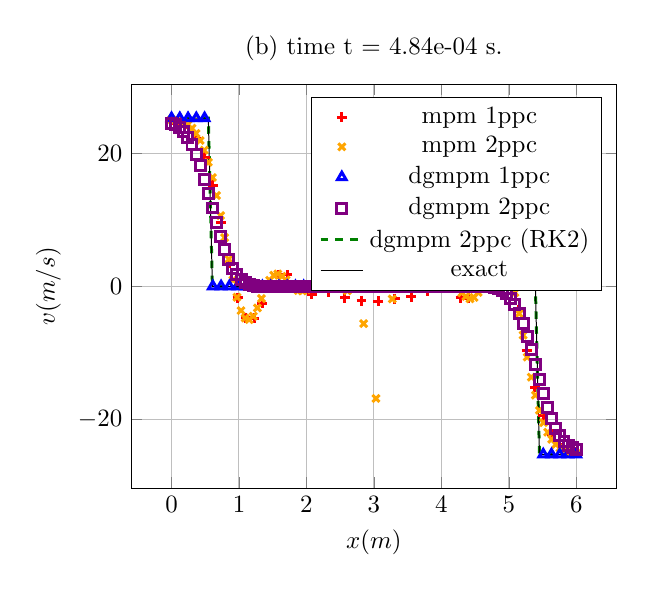
\begin{tikzpicture}[scale=0.9]
\begin{axis}[xlabel=$x (m)$,ylabel=$v (m/s)$,ymajorgrids=true,xmajorgrids=true,legend pos=north east,title={(b) time t = 4.84e-04 s.}]
\addplot[Red,very thick,mark=+,only marks] coordinates {(0.0,25.010841927729743) (0.12244897959183673,24.69190114266878) (0.24489795918367346,23.885243262511448) (0.36734693877551017,22.273018421403247) (0.4897959183673469,19.469489967062028) (0.6122448979591837,15.21098253183553) (0.7346938775510203,9.639084261801766) (0.8571428571428571,3.535042674142188) (0.9795918367346939,-1.734652221822011) (1.1020408163265305,-4.738949800515776) (1.2244897959183674,-4.781129013135261) (1.346938775510204,-2.546047420872023) (1.4693877551020407,0.3038529149069791) (1.5918367346938775,1.7867317133486076) (1.7142857142857142,1.731851964763841) (1.836734693877551,0.09715941997364874) (1.9591836734693877,-0.2832074608631421) (2.0816326530612246,-1.2253977208566522) (2.204081632653061,0.7014518615294985) (2.326530612244898,-0.7977872830116236) (2.4489795918367347,1.588281886075272) (2.571428571428571,-1.7170093073527637) (2.693877551020408,1.8355506260116217) (2.816326530612245,-2.148933313216083) (2.9387755102040813,2.2532520111024343) (3.061224489795918,-2.2532520111024077) (3.183673469387755,2.148933313216088) (3.306122448979592,-1.8355506260115833) (3.4285714285714284,1.7170093073527628) (3.5510204081632653,-1.5882818860752659) (3.673469387755102,0.7977872830116278) (3.7959183673469385,-0.7014518615294782) (3.9183673469387754,1.225397720856666) (4.040816326530612,0.2832074608631516) (4.163265306122449,-0.09715941997367494) (4.285714285714286,-1.7318519647638575) (4.408163265306122,-1.7867317133486047) (4.530612244897959,-0.3038529149069491) (4.653061224489796,2.5460474208720303) (4.775510204081632,4.781129013135254) (4.8979591836734695,4.738949800515773) (5.020408163265306,1.734652221822016) (5.142857142857142,-3.5350426741421663) (5.26530612244898,-9.639084261801804) (5.387755102040816,-15.210982531835537) (5.5102040816326525,-19.46948996706204) (5.63265306122449,-22.273018421403254) (5.755102040816326,-23.885243262511455) (5.877551020408163,-24.691901142668783) (6.0,-25.01084192772974) };
\addplot[Orange,very thick,mark=x,only marks] coordinates {(0.0,25.129222896014145) (0.06060606060606061,25.07159803666336) (0.12121212121212122,24.933072053261906) (0.18181818181818182,24.713644945809776) (0.24242424242424243,24.341811221412843) (0.30303030303030304,23.81757088007112) (0.36363636363636365,23.025842175877788) (0.42424242424242425,21.966625108832844) (0.48484848484848486,20.51636723745046) (0.5454545454545454,18.675068561730647) (0.6060606060606061,16.3951416558921) (0.6666666666666667,13.676586519934855) (0.7272727272727273,10.659200652949888) (0.7878787878787878,7.342984054937215) (0.8484848484848485,4.1056664759142745) (0.9090909090909092,0.9472479158810896) (0.9696969696969697,-1.6372314354382502) (1.0303030303030303,-3.647771578043734) (1.0909090909090908,-4.770448939067272) (1.1515151515151516,-5.005263518508844) (1.2121212121212122,-4.498657239486039) (1.2727272727272727,-3.2506301019988686) (1.3333333333333335,-1.8348993400450033) (1.393939393939394,-0.25146495362441823) (1.4545454545454546,0.9159748054237657) (1.5151515151515151,1.6674199370995528) (1.5757575757575757,1.869108998638306) (1.6363636363636365,1.5210419900399856) (1.696969696969697,0.9751485230255432) (1.7575757575757576,0.2314285975949515) (1.8181818181818183,-0.3040337277600307) (1.878787878787879,-0.6312384530394275) (1.9393939393939394,-0.6886040223069566) (2.0,-0.47613043556259904) (2.0606060606060606,-0.23072733446746102) (2.121212121212121,0.04760528097847652) (2.1818181818181817,0.2118520367643768) (2.2424242424242427,0.2620129328902514) (2.303030303030303,0.1893864845926331) (2.3636363636363638,-0.006027308128489575) (2.4242424242424243,-0.02569518359528772) (2.484848484848485,0.13038285819222342) (2.5454545454545454,-0.08413298428170798) (2.606060606060606,-0.669242711017074) (2.666666666666667,-0.009936080373916245) (2.7272727272727275,1.893786907647783) (2.787878787878788,0.02845356832822474) (2.8484848484848486,-5.605936098332585) (2.909090909090909,0.012272845525669835) (2.9696969696969697,16.883080399903026) (3.0303030303030303,-16.88308039990298) (3.090909090909091,-0.012272845525692286) (3.1515151515151514,5.605936098332596) (3.2121212121212124,-0.028453568328220977) (3.272727272727273,-1.8937869076477436) (3.3333333333333335,0.009936080373926855) (3.393939393939394,0.6692427110170838) (3.4545454545454546,0.08413298428171725) (3.515151515151515,-0.13038285819221412) (3.5757575757575757,0.025695183595291035) (3.6363636363636367,0.006027308128479805) (3.6969696969696972,-0.1893864845926492) (3.757575757575758,-0.262012932890273) (3.8181818181818183,-0.21185203676439526) (3.878787878787879,-0.04760528097849795) (3.9393939393939394,0.23072733446744584) (4.0,0.47613043556258583) (4.0606060606060606,0.6886040223069541) (4.121212121212121,0.6312384530394359) (4.181818181818182,0.3040337277600474) (4.242424242424242,-0.23142859759493706) (4.303030303030303,-0.9751485230255246) (4.363636363636363,-1.5210419900399839) (4.424242424242425,-1.86910899863831) (4.484848484848485,-1.6674199370995695) (4.545454545454546,-0.9159748054237709) (4.606060606060606,0.25146495362442267) (4.666666666666667,1.8348993400449871) (4.7272727272727275,3.250630101998864) (4.787878787878788,4.498657239486027) (4.848484848484849,5.005263518508832) (4.909090909090909,4.7704489390672595) (4.96969696969697,3.6477715780437387) (5.03030303030303,1.6372314354382556) (5.090909090909091,-0.9472479158810874) (5.151515151515151,-4.10566647591428) (5.212121212121212,-7.34298405493721) (5.2727272727272725,-10.659200652949886) (5.333333333333334,-13.676586519934842) (5.3939393939393945,-16.39514165589211) (5.454545454545455,-18.675068561730637) (5.515151515151516,-20.516367237450467) (5.575757575757576,-21.96662510883284) (5.636363636363637,-23.025842175877788) (5.696969696969697,-23.817570880071123) (5.757575757575758,-24.341811221412847) (5.818181818181818,-24.71364494580977) (5.878787878787879,-24.933072053261906) (5.9393939393939394,-25.07159803666337) (6.0,-25.12922289601414) };
\addplot[Blue,very thick,mark=triangle,only marks] coordinates {(0.0,25.318484177091673) (0.12244897959183673,25.31848417709167) (0.24489795918367346,25.318484177091673) (0.36734693877551017,25.318484177091676) (0.4897959183673469,25.31848417709167) (0.6122448979591837,-1.5987211554602254e-14) (0.7346938775510203,2.3249369091697067e-14) (0.8571428571428571,-1.2969013043348462e-14) (0.9795918367346939,1.7212972069189483e-14) (1.1020408163265305,-1.5987211554602254e-14) (1.2244897959183674,1.6143941734096062e-14) (1.346938775510204,-1.5279885050295412e-14) (1.4693877551020407,1.7920298573496322e-14) (1.5918367346938775,-1.900541006585605e-14) (1.7142857142857142,1.6505645564882647e-14) (1.836734693877551,-1.9712736570162884e-14) (1.9591836734693877,1.6505645564882647e-14) (2.0816326530612246,-1.616002289136238e-14) (2.204081632653061,1.4194773557935691e-14) (2.326530612244898,-1.971273657016288e-14) (2.4489795918367347,1.6867349395669235e-14) (2.571428571428571,-1.7574675899976055e-14) (2.693877551020408,1.260730921256188e-14) (2.816326530612245,-1.5625507723815666e-14) (2.9387755102040813,1.1538278877468474e-14) (3.061224489795918,-1.455647738872226e-14) (3.183673469387755,9.58911070130809e-15) (3.306122448979592,-4.967366687414162e-15) (3.4285714285714284,6.036397022507581e-15) (3.5510204081632653,-7.278238694361135e-15) (3.673469387755102,6.570912190054291e-15) (3.7959183673469385,-7.985565198667975e-15) (3.9183673469387754,7.105427357601003e-15) (4.040816326530612,-1.1003763709921776e-14) (4.163265306122449,8.88178419700125e-15) (4.285714285714286,-9.227406870521513e-15) (4.408163265306122,2.845387174493662e-15) (4.530612244897959,-6.2092083592677194e-15) (4.653061224489796,2.8453871744936586e-15) (4.775510204081632,-6.209208359267724e-15) (4.8979591836734695,5.863585685747457e-15) (5.020408163265306,-6.209208359267721e-15) (5.142857142857142,2.8453871744936617e-15) (5.26530612244898,-1.728113367601308e-16) (5.387755102040816,8.881784197001252e-15) (5.5102040816326525,-25.31848417709167) (5.63265306122449,-25.318484177091673) (5.755102040816326,-25.318484177091662) (5.877551020408163,-25.318484177091673) (6.0,-25.31848417709167) };
\addplot[Purple,very thick,mark=square,only marks] coordinates {(0.0,24.50287887963811) (0.06060606060606061,24.33115661714126) (0.12121212121212122,23.91224984156279) (0.18181818181818182,23.343290482677553) (0.24242424242424243,22.418909444576503) (0.30303030303030304,21.33656683027461) (0.36363636363636365,19.82993211922009) (0.42424242424242425,18.174087611146433) (0.48484848484848486,16.15477586747816) (0.5454545454545454,14.047401021710659) (0.6060606060606061,11.801065385155283) (0.6666666666666667,9.574083982688228) (0.7272727272727273,7.516285480780097) (0.7878787878787878,5.581100772293223) (0.8484848484848485,4.051002927700874) (0.9090909090909092,2.6880573007181487) (0.9696969696969697,1.7842696860673242) (1.0303030303030303,1.022292062977273) (1.0909090909090908,0.612397359894627) (1.1515151515151516,0.28491831319579164) (1.2121212121212122,0.15077503968818412) (1.2727272727272727,0.04852500743676242) (1.3333333333333335,0.021327686188368628) (1.393939393939394,0.0009497890449827739) (1.4545454545454546,-0.0003613906028922416) (1.5151515151515151,-0.0017718830663082294) (1.5757575757575757,-0.0008197840812235387) (1.6363636363636365,-0.0003778569739121728) (1.696969696969697,-0.00013168311989373) (1.7575757575757576,-7.18048229836903e-06) (1.8181818181818183,1.252516158948592e-06) (1.878787878787879,7.5714301535093654e-06) (1.9393939393939394,2.4486602184000188e-06) (2.0,7.135513792355919e-07) (2.0606060606060606,1.4595492173879264e-07) (2.121212121212121,-6.36315439268717e-08) (2.1818181818181817,-1.837735247302598e-08) (2.2424242424242427,-9.0259024175961e-09) (2.303030303030303,-1.5217928776877251e-09) (2.3636363636363638,3.101587594170799e-10) (2.4242424242424243,7.24127604304446e-11) (2.484848484848485,4.4976117597291944e-11) (2.5454545454545454,5.002147690366477e-12) (2.606060606060606,-1.0802191013820454e-12) (2.666666666666667,-1.4990751315243186e-13) (2.7272727272727275,-8.117792812779083e-14) (2.787878787878788,-1.0886141133533906e-14) (2.8484848484848486,-3.827845768442499e-15) (2.909090909090909,-7.56064137928349e-15) (2.9696969696969697,-5.503253411831473e-15) (3.0303030303030303,-3.863692389725438e-15) (3.090909090909091,-5.870869032280005e-15) (3.1515151515151514,-1.6142354040084839e-15) (3.2121212121212124,4.421215058875589e-15) (3.272727272727273,7.8614872769933e-14) (3.3333333333333335,1.4955283737379606e-13) (3.393939393939394,1.0765053855759234e-12) (3.4545454545454546,-5.0045785030174495e-12) (3.515151515151515,-4.4973577805717606e-11) (3.5757575757575757,-7.241313743047312e-11) (3.6363636363636367,-3.1016637178276513e-10) (3.6969696969696972,1.5217866709738466e-09) (3.757575757575758,9.02588784622573e-09) (3.8181818181818183,1.83773394376186e-08) (3.878787878787879,6.36315292704854e-08) (3.9393939393939394,-1.4595493373975597e-07) (4.0,-7.135513899230807e-07) (4.0606060606060606,-2.4486602364102843e-06) (4.121212121212121,-7.571430174183029e-06) (4.181818181818182,-1.2525161868276612e-06) (4.242424242424242,7.1804822724005926e-06) (4.303030303030303,0.0001316831198674206) (4.363636363636363,0.0003778569738877074) (4.424242424242425,0.0008197840811925695) (4.484848484848485,0.0017718830662707546) (4.545454545454546,0.0003613906028578342) (4.606060606060606,-0.0009497890450032697) (4.666666666666667,-0.021327686188389254) (4.7272727272727275,-0.04852500743678493) (4.787878787878788,-0.15077503968820735) (4.848484848484849,-0.28491831319581384) (4.909090909090909,-0.6123973598946483) (4.96969696969697,-1.0222920629772922) (5.03030303030303,-1.7842696860673455) (5.090909090909091,-2.688057300718164) (5.151515151515151,-4.051002927700886) (5.212121212121212,-5.58110077229324) (5.2727272727272725,-7.516285480780111) (5.333333333333334,-9.574083982688242) (5.3939393939393945,-11.801065385155285) (5.454545454545455,-14.04740102171067) (5.515151515151516,-16.15477586747817) (5.575757575757576,-18.17408761114645) (5.636363636363637,-19.8299321192201) (5.696969696969697,-21.336566830274624) (5.757575757575758,-22.418909444576517) (5.818181818181818,-23.343290482677574) (5.878787878787879,-23.912249841562804) (5.9393939393939394,-24.33115661714127) (6.0,-24.502878879638118) };
\addplot[Green,very thick,mark=none,dashed] coordinates {(0.0,25.318484177091655) (0.06060606060606061,25.31848417709166) (0.12121212121212122,25.31848417709171) (0.18181818181818182,25.31848417709171) (0.24242424242424243,25.318484177091648) (0.30303030303030304,25.318484177091655) (0.36363636363636365,25.31848417709169) (0.42424242424242425,25.31848417709169) (0.48484848484848486,25.318484177091662) (0.5454545454545454,25.318484177091662) (0.6060606060606061,-2.0428103653102877e-14) (0.6666666666666667,-2.5757174171303635e-14) (0.7272727272727273,-9.37411687865018e-16) (0.7878787878787878,2.1400402629190024e-16) (0.8484848484848485,2.0475064051554806e-14) (0.9090909090909092,1.9609492121278842e-14) (0.9696969696969697,-3.22146132403454e-14) (1.0303030303030303,-3.704722233899802e-14) (1.0909090909090908,-1.97136343382622e-14) (1.1515151515151516,-2.1504276798730107e-14) (1.2121212121212122,-1.0526619956320885e-14) (1.2727272727272727,-5.131050082027361e-15) (1.3333333333333335,1.4158260986553617e-14) (1.393939393939394,1.2438848132651247e-14) (1.4545454545454546,-2.7664379544035256e-14) (1.5151515151515151,-2.2797019620744853e-14) (1.5757575757575757,-8.03242851712116e-15) (1.6363636363636365,-8.654368371463993e-16) (1.696969696969697,4.664670837723429e-15) (1.7575757575757576,2.7863791933978877e-15) (1.8181818181818183,-1.0404944920045015e-14) (1.878787878787879,-1.5533081166651847e-14) (1.9393939393939394,-3.666195759453223e-15) (2.0,-2.0245785895340724e-15) (2.0606060606060606,-1.1061335980362311e-14) (2.121212121212121,-7.047855087160429e-15) (2.1818181818181817,3.616841638731114e-15) (2.2424242424242427,-6.412795993019872e-17) (2.303030303030303,-3.39260543187031e-14) (2.3636363636363638,-3.744167961629452e-14) (2.4242424242424243,7.917549738276896e-15) (2.484848484848485,8.776988320632252e-15) (2.5454545454545454,-1.167164224722479e-14) (2.606060606060606,-1.1059292834191826e-14) (2.666666666666667,-1.1996100398551465e-14) (2.7272727272727275,-1.3218518026572238e-14) (2.787878787878788,9.96260825263207e-15) (2.8484848484848486,9.215613149984149e-15) (2.909090909090909,-1.1610134928643289e-14) (2.9696969696969697,-1.1466422826293636e-14) (3.0303030303030303,6.046764652828676e-16) (3.090909090909091,4.362690222131271e-15) (3.1515151515151514,1.6201412864530872e-15) (3.2121212121212124,8.635420572536498e-16) (3.272727272727273,1.6940449921659094e-16) (3.3333333333333335,2.314278844490485e-15) (3.393939393939394,1.877668370403333e-15) (3.4545454545454546,4.158728652104211e-15) (3.515151515151515,-5.301949675286611e-15) (3.5757575757575757,-4.632783699541811e-15) (3.6363636363636367,-4.5621868425192295e-15) (3.6969696969696972,-3.957893523695509e-15) (3.757575757575758,-1.4287835984024765e-14) (3.8181818181818183,-1.1995812776192492e-14) (3.878787878787879,1.5282013805742645e-15) (3.9393939393939394,4.5081956419332734e-15) (4.0,-4.63661483338482e-15) (4.0606060606060606,-3.883465532829902e-15) (4.121212121212121,-1.597445999358722e-15) (4.181818181818182,-6.231389019815505e-15) (4.242424242424242,-4.3312542293455905e-15) (4.303030303030303,-1.3595201196418142e-15) (4.363636363636363,-8.725822124812144e-15) (4.424242424242425,-5.139409916871529e-15) (4.484848484848485,1.8303622166233665e-15) (4.545454545454546,-1.1391168695828289e-15) (4.606060606060606,-6.7379551610850494e-15) (4.666666666666667,-7.127276880596735e-15) (4.7272727272727275,-1.875997519087127e-14) (4.787878787878788,-1.7836191932227193e-14) (4.848484848484849,-1.5790231922526684e-16) (4.909090909090909,8.491476662657315e-16) (4.96969696969697,1.0692862618066636e-14) (5.03030303030303,6.6929207878829085e-15) (5.090909090909091,-9.61372733539056e-15) (5.151515151515151,-1.0633524402319082e-14) (5.212121212121212,-9.111869380559471e-15) (5.2727272727272725,-5.822392996215753e-15) (5.333333333333334,-2.39808173319034e-14) (5.3939393939393945,1.3322676295501828e-14) (5.454545454545455,-25.318484177091683) (5.515151515151516,-25.318484177091687) (5.575757575757576,-25.318484177091662) (5.636363636363637,-25.318484177091662) (5.696969696969697,-25.318484177091698) (5.757575757575758,-25.3184841770917) (5.818181818181818,-25.31848417709168) (5.878787878787879,-25.318484177091687) (5.9393939393939394,-25.318484177091694) (6.0,-25.318484177091698) };
\addplot[black,thin,mark=none,solid] coordinates {(0.0,25.318484177091666) (0.06060606060606061,25.318484177091666) (0.12121212121212122,25.318484177091666) (0.18181818181818182,25.318484177091666) (0.24242424242424243,25.318484177091666) (0.30303030303030304,25.318484177091666) (0.36363636363636365,25.318484177091666) (0.42424242424242425,25.318484177091666) (0.48484848484848486,25.318484177091666) (0.5454545454545454,25.318484177091666) (0.6060606060606061,0.0) (0.6666666666666667,0.0) (0.7272727272727273,0.0) (0.7878787878787878,0.0) (0.8484848484848485,0.0) (0.9090909090909092,0.0) (0.9696969696969697,0.0) (1.0303030303030303,0.0) (1.0909090909090908,0.0) (1.1515151515151516,0.0) (1.2121212121212122,0.0) (1.2727272727272727,0.0) (1.3333333333333335,0.0) (1.393939393939394,0.0) (1.4545454545454546,0.0) (1.5151515151515151,0.0) (1.5757575757575757,0.0) (1.6363636363636365,0.0) (1.696969696969697,0.0) (1.7575757575757576,0.0) (1.8181818181818183,0.0) (1.878787878787879,0.0) (1.9393939393939394,0.0) (2.0,0.0) (2.0606060606060606,0.0) (2.121212121212121,0.0) (2.1818181818181817,0.0) (2.2424242424242427,0.0) (2.303030303030303,0.0) (2.3636363636363638,0.0) (2.4242424242424243,0.0) (2.484848484848485,0.0) (2.5454545454545454,0.0) (2.606060606060606,0.0) (2.666666666666667,0.0) (2.7272727272727275,0.0) (2.787878787878788,0.0) (2.8484848484848486,0.0) (2.909090909090909,0.0) (2.9696969696969697,0.0) (3.0303030303030303,-0.0) (3.090909090909091,-0.0) (3.1515151515151514,-0.0) (3.2121212121212124,-0.0) (3.272727272727273,-0.0) (3.3333333333333335,-0.0) (3.393939393939394,-0.0) (3.4545454545454546,-0.0) (3.515151515151515,-0.0) (3.5757575757575757,-0.0) (3.6363636363636367,-0.0) (3.6969696969696972,-0.0) (3.757575757575758,-0.0) (3.8181818181818183,-0.0) (3.878787878787879,-0.0) (3.9393939393939394,-0.0) (4.0,-0.0) (4.0606060606060606,-0.0) (4.121212121212121,-0.0) (4.181818181818182,-0.0) (4.242424242424242,-0.0) (4.303030303030303,-0.0) (4.363636363636363,-0.0) (4.424242424242425,-0.0) (4.484848484848485,-0.0) (4.545454545454546,-0.0) (4.606060606060606,-0.0) (4.666666666666667,-0.0) (4.7272727272727275,-0.0) (4.787878787878788,-0.0) (4.848484848484849,-0.0) (4.909090909090909,-0.0) (4.96969696969697,-0.0) (5.03030303030303,-0.0) (5.090909090909091,-0.0) (5.151515151515151,-0.0) (5.212121212121212,-0.0) (5.2727272727272725,-0.0) (5.333333333333334,-0.0) (5.3939393939393945,-0.0) (5.454545454545455,-25.318484177091666) (5.515151515151516,-25.318484177091666) (5.575757575757576,-25.318484177091666) (5.636363636363637,-25.318484177091666) (5.696969696969697,-25.318484177091666) (5.757575757575758,-25.318484177091666) (5.818181818181818,-25.318484177091666) (5.878787878787879,-25.318484177091666) (5.9393939393939394,-25.318484177091666) (6.0,-25.318484177091666) };
\legend{mpm 1ppc,mpm 2ppc,dgmpm 1ppc,dgmpm 2ppc,dgmpm 2ppc (RK2),exact}
\end{axis}
\end{tikzpicture}
%%% Local Variables:
%%% mode: latex
%%% TeX-master: "../../mainManuscript"
%%% End:
}
 \caption{elastic RP velo}
  \label{fig:velo_elastic_RP}
\end{figure}

\subsection{One-dimensional elastoviscoplasticity}
\subsection{One-dimensional elastoplasticity}
Comparison with mpm for 1ppc
\begin{figure}[h!]
  \centering
  {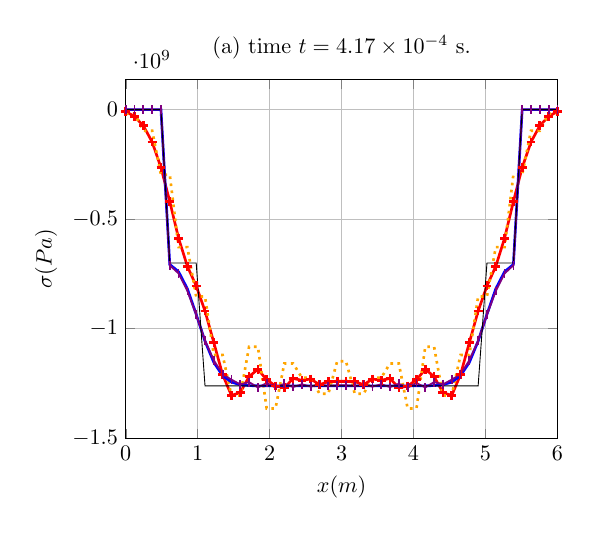
\begin{tikzpicture}[scale=0.8]
\begin{axis}[xlabel=$x (m)$,ylabel=$\sigma (Pa)$,ymajorgrids=true,xmajorgrids=true,legend pos=outer north east,title={(a) time $t = 4.17\times 10^{-4} $ s.},xmin=0.,xmax=6.]
\addplot[Red,very thick,mark=+,solid] coordinates {(0.0,-8433215.03790355) (0.12244897959183673,-31379937.150059074) (0.24489795918367346,-73325965.87671247) (0.36734693877551017,-147815909.35881704) (0.4897959183673469,-264501011.32373637) (0.6122448979591837,-419797360.6339785) (0.7346938775510203,-586994803.1537646) (0.8571428571428571,-715242874.2277462) (0.9795918367346939,-804731796.1198385) (1.1020408163265305,-919403784.9173691) (1.2244897959183674,-1063504114.033879) (1.346938775510204,-1209904754.949398) (1.4693877551020407,-1304654513.0867395) (1.5918367346938775,-1291382612.5749428) (1.7142857142857142,-1218226204.6353252) (1.836734693877551,-1185455835.0777807) (1.9591836734693877,-1232745182.470082) (2.0816326530612246,-1261396271.0817113) (2.204081632653061,-1270103667.4391637) (2.326530612244898,-1227250869.598082) (2.4489795918367347,-1235273389.504192) (2.571428571428571,-1229787858.686364) (2.693877551020408,-1255621316.42765) (2.816326530612245,-1241442333.7811728) (2.9387755102040813,-1239848703.7218106) (3.061224489795918,-1239848703.7218091) (3.183673469387755,-1241442333.781176) (3.306122448979592,-1255621316.4276485) (3.4285714285714284,-1229787858.6863654) (3.5510204081632653,-1235273389.5041904) (3.673469387755102,-1227250869.598084) (3.7959183673469385,-1270103667.439164) (3.9183673469387754,-1261396271.081712) (4.040816326530612,-1232745182.4700806) (4.163265306122449,-1185455835.0777805) (4.285714285714286,-1218226204.6353254) (4.408163265306122,-1291382612.5749435) (4.530612244897959,-1304654513.0867395) (4.653061224489796,-1209904754.9493968) (4.775510204081632,-1063504114.033878) (4.8979591836734695,-919403784.917369) (5.020408163265306,-804731796.1198374) (5.142857142857142,-715242874.2277458) (5.26530612244898,-586994803.1537648) (5.387755102040816,-419797360.63397753) (5.5102040816326525,-264501011.3237358) (5.63265306122449,-147815909.35881624) (5.755102040816326,-73325965.8767119) (5.877551020408163,-31379937.150058918) (6.0,-8433215.037903389) };
\addplot[Orange,very thick,mark=none,dotted] coordinates {(0.0,-19024028.854669835) (0.12244897959183673,-19024028.85467063) (0.24489795918367346,-96232491.2346082) (0.36734693877551017,-96232491.2346095) (0.4897959183673469,-297240710.94206506) (0.6122448979591837,-297240710.94206476) (0.7346938775510203,-627598280.4404582) (0.8571428571428571,-627598280.4404559) (0.9795918367346939,-853300561.8320081) (1.1020408163265305,-853300561.8320053) (1.2244897959183674,-1120326134.4042003) (1.346938775510204,-1120326134.4041946) (1.4693877551020407,-1305012184.0617018) (1.5918367346938775,-1305012184.061693) (1.7142857142857142,-1082408762.037375) (1.836734693877551,-1082408762.0373683) (1.9591836734693877,-1364071875.0838804) (2.0816326530612246,-1364071875.083866) (2.204081632653061,-1158492862.0093477) (2.326530612244898,-1158492862.0093355) (2.4489795918367347,-1223885693.6431794) (2.571428571428571,-1223885693.6431704) (2.693877551020408,-1296923820.0786731) (2.816326530612245,-1296923820.0786521) (2.9387755102040813,-1148570801.226303) (3.061224489795918,-1148570801.2262988) (3.183673469387755,-1296923820.0786695) (3.306122448979592,-1296923820.0786562) (3.4285714285714284,-1223885693.6431804) (3.5510204081632653,-1223885693.643168) (3.673469387755102,-1158492862.009347) (3.7959183673469385,-1158492862.0093367) (3.9183673469387754,-1364071875.083883) (4.040816326530612,-1364071875.0838625) (4.163265306122449,-1082408762.0373764) (4.285714285714286,-1082408762.0373673) (4.408163265306122,-1305012184.061705) (4.530612244897959,-1305012184.061689) (4.653061224489796,-1120326134.4042025) (4.775510204081632,-1120326134.4041922) (4.8979591836734695,-853300561.8320092) (5.020408163265306,-853300561.8320037) (5.142857142857142,-627598280.440458) (5.26530612244898,-627598280.440457) (5.387755102040816,-297240710.9420676) (5.5102040816326525,-297240710.9420631) (5.63265306122449,-96232491.23461069) (5.755102040816326,-96232491.23460749) (5.877551020408163,-19024028.85467079) (6.0,-19024028.85467007) };
\addplot[Blue,very thick,mark=none,solid] coordinates {(0.0,-3.2561158711216654e-07) (0.12244897959183673,-6.54162606232603e-22) (0.24489795918367346,0.0) (0.36734693877551017,3.2561158711216643e-07) (0.4897959183673469,-4.884173806682499e-07) (0.6122448979591837,-706703995.0062007) (0.7346938775510203,-739923853.3127105) (0.8571428571428571,-818114621.3278772) (0.9795918367346939,-934350667.0858994) (1.1020408163265305,-1056745717.4113452) (1.2244897959183674,-1153785079.176232) (1.346938775510204,-1213891661.9862223) (1.4693877551020407,-1243675875.166416) (1.5918367346938775,-1255667377.4619899) (1.7142857142857142,-1259628756.7765899) (1.836734693877551,-1260708382.472525) (1.9591836734693877,-1260951555.06527) (2.0816326530612246,-1260996741.6987677) (2.204081632653061,-1261003631.246593) (2.326530612244898,-1261004484.7294881) (2.4489795918367347,-1261004569.3136225) (2.571428571428571,-1261004575.8625927) (2.693877551020408,-1261004576.2443771) (2.816326530612245,-1261004576.2601426) (2.9387755102040813,-1261004576.2605536) (3.061224489795918,-1261004576.2605536) (3.183673469387755,-1261004576.2601426) (3.306122448979592,-1261004576.2443776) (3.4285714285714284,-1261004575.862593) (3.5510204081632653,-1261004569.3136227) (3.673469387755102,-1261004484.7294881) (3.7959183673469385,-1261003631.2465928) (3.9183673469387754,-1260996741.6987677) (4.040816326530612,-1260951555.0652697) (4.163265306122449,-1260708382.4725246) (4.285714285714286,-1259628756.7765894) (4.408163265306122,-1255667377.4619899) (4.530612244897959,-1243675875.1664157) (4.653061224489796,-1213891661.9862223) (4.775510204081632,-1153785079.176232) (4.8979591836734695,-1056745717.4113454) (5.020408163265306,-934350667.0858992) (5.142857142857142,-818114621.327877) (5.26530612244898,-739923853.3127109) (5.387755102040816,-706703995.0062011) (5.5102040816326525,-4.884173806682498e-07) (5.63265306122449,0.0) (5.755102040816326,-4.884173806682498e-07) (5.877551020408163,0.0) (6.0,-4.884173806682498e-07) };
\addplot[Purple,thick,mark=|,solid] coordinates {(0.0,-3.2561158711216654e-07) (0.12244897959183673,-6.54162606232603e-22) (0.24489795918367346,0.0) (0.36734693877551017,3.2561158711216643e-07) (0.4897959183673469,-4.884173806682499e-07) (0.6122448979591837,-710637837.2357953) (0.7346938775510203,-747893724.781927) (0.8571428571428571,-827829409.8631966) (0.9795918367346939,-936780409.853217) (1.1020408163265305,-1054073198.2499647) (1.2244897959183674,-1144128439.1849532) (1.346938775510204,-1207925723.6670742) (1.4693877551020407,-1232372577.7948787) (1.5918367346938775,-1254253728.274747) (1.7142857142857142,-1243570946.3490026) (1.836734693877551,-1268139963.2569304) (1.9591836734693877,-1248035262.8872383) (2.0816326530612246,-1268992337.693115) (2.204081632653061,-1251285653.8729925) (2.326530612244898,-1266352346.5241969) (2.4489795918367347,-1253527311.8706975) (2.571428571428571,-1264419055.233534) (2.693877551020408,-1255474245.0991223) (2.816326530612245,-1261578869.0693417) (2.9387755102040813,-1258168698.6750736) (3.061224489795918,-1258168698.6750731) (3.183673469387755,-1261578869.069342) (3.306122448979592,-1255474245.0991209) (3.4285714285714284,-1264419055.233534) (3.5510204081632653,-1253527311.870696) (3.673469387755102,-1266352346.5241973) (3.7959183673469385,-1251285653.8729923) (3.9183673469387754,-1268992337.6931143) (4.040816326530612,-1248035262.8872375) (4.163265306122449,-1268139963.2569308) (4.285714285714286,-1243570946.3490026) (4.408163265306122,-1254253728.2747467) (4.530612244897959,-1232372577.7948787) (4.653061224489796,-1207925723.6670735) (4.775510204081632,-1144128439.1849532) (4.8979591836734695,-1054073198.2499645) (5.020408163265306,-936780409.853217) (5.142857142857142,-827829409.8631967) (5.26530612244898,-747893724.7819276) (5.387755102040816,-710637837.2357956) (5.5102040816326525,-4.884173806682498e-07) (5.63265306122449,0.0) (5.755102040816326,-4.884173806682498e-07) (5.877551020408163,0.0) (6.0,-4.884173806682498e-07) };
\addplot[black,thin,mark=none,solid] coordinates {(0.0,-0.0) (0.12244897959183673,-0.0) (0.24489795918367346,-0.0) (0.36734693877551017,-0.0) (0.4897959183673469,-0.0) (0.6122448979591837,-700000000.0) (0.7346938775510203,-700000000.0) (0.8571428571428571,-700000000.0) (0.9795918367346939,-700000000.0) (1.1020408163265305,-1261004576.260559) (1.2244897959183674,-1261004576.260559) (1.346938775510204,-1261004576.260559) (1.4693877551020407,-1261004576.260559) (1.5918367346938775,-1261004576.260559) (1.7142857142857142,-1261004576.260559) (1.836734693877551,-1261004576.260559) (1.9591836734693877,-1261004576.260559) (2.0816326530612246,-1261004576.260559) (2.204081632653061,-1261004576.260559) (2.326530612244898,-1261004576.260559) (2.4489795918367347,-1261004576.260559) (2.571428571428571,-1261004576.260559) (2.693877551020408,-1261004576.260559) (2.816326530612245,-1261004576.260559) (2.9387755102040813,-1261004576.260559) (3.061224489795918,-1261004576.260559) (3.183673469387755,-1261004576.260559) (3.306122448979592,-1261004576.260559) (3.4285714285714284,-1261004576.260559) (3.5510204081632653,-1261004576.260559) (3.673469387755102,-1261004576.260559) (3.7959183673469385,-1261004576.260559) (3.9183673469387754,-1261004576.260559) (4.040816326530612,-1261004576.260559) (4.163265306122449,-1261004576.260559) (4.285714285714286,-1261004576.260559) (4.408163265306122,-1261004576.260559) (4.530612244897959,-1261004576.260559) (4.653061224489796,-1261004576.260559) (4.775510204081632,-1261004576.260559) (4.8979591836734695,-1261004576.260559) (5.020408163265306,-700000000.0) (5.142857142857142,-700000000.0) (5.26530612244898,-700000000.0) (5.387755102040816,-700000000.0) (5.5102040816326525,-0.0) (5.63265306122449,-0.0) (5.755102040816326,-0.0) (5.877551020408163,-0.0) (6.0,-0.0) };
%\legend{usl,usf,dgmpm (ep solver),dgmpm (ac solver),exact}
\end{axis}
\end{tikzpicture}
%%% Local Variables:
%%% mode: latex
%%% TeX-master: "../../mainManuscript"
%%% End:
}
  {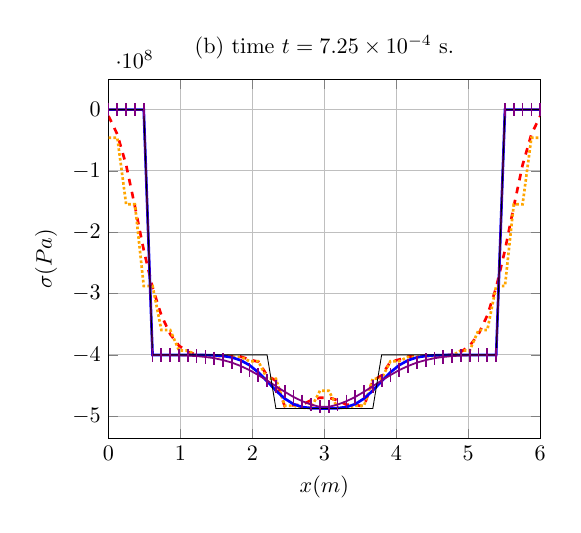
\begin{tikzpicture}[scale=0.8]
\begin{axis}[xlabel=$x (m)$,ylabel=$\sigma (Pa)$,ymajorgrids=true,xmajorgrids=true,legend pos=outer north east,title={(b) time $t = 7.25\times 10^{-4} $ s.},xmin=0.,xmax=6.]
\addplot[Red,very thick,mark=none,dashed,mark size=3pt] coordinates {(0.0,-10477027.22040739) (0.12244897959183673,-40202439.77672757) (0.24489795918367346,-90268409.98400429) (0.36734693877551017,-157917330.96394995) (0.4897959183673469,-229098117.24026006) (0.6122448979591837,-290170966.79273176) (0.7346938775510203,-335449952.79523534) (0.8571428571428571,-366063963.8356788) (0.9795918367346939,-384934670.81956863) (1.1020408163265305,-394978768.22705775) (1.2244897959183674,-399539747.49342227) (1.346938775510204,-401064801.98949975) (1.4693877551020407,-401261686.3649931) (1.5918367346938775,-401362011.1717392) (1.7142857142857142,-402125702.7814173) (1.836734693877551,-402648608.50963366) (1.9591836734693877,-407517028.59914577) (2.0816326530612246,-411133976.99807984) (2.204081632653061,-433339939.374477) (2.326530612244898,-442099776.2163934) (2.4489795918367347,-483576545.68129754) (2.571428571428571,-481854124.4484605) (2.693877551020408,-481095256.73223835) (2.816326530612245,-473792554.1947772) (2.9387755102040813,-469732138.6842222) (3.061224489795918,-469732138.6842212) (3.183673469387755,-473792554.1947779) (3.306122448979592,-481095256.73223734) (3.4285714285714284,-481854124.4484616) (3.5510204081632653,-483576545.6812961) (3.673469387755102,-442099776.2163934) (3.7959183673469385,-433339939.3744765) (3.9183673469387754,-411133976.99807984) (4.040816326530612,-407517028.5991456) (4.163265306122449,-402648608.50963354) (4.285714285714286,-402125702.78141725) (4.408163265306122,-401362011.1717393) (4.530612244897959,-401261686.3649931) (4.653061224489796,-401064801.9894998) (4.775510204081632,-399539747.4934223) (4.8979591836734695,-394978768.22705775) (5.020408163265306,-384934670.81956846) (5.142857142857142,-366063963.83567846) (5.26530612244898,-335449952.79523504) (5.387755102040816,-290170966.7927308) (5.5102040816326525,-229098117.24025902) (5.63265306122449,-157917330.96394882) (5.755102040816326,-90268409.98400334) (5.877551020408163,-40202439.77672676) (6.0,-10477027.22040709) };
\addplot[Orange,very thick,mark=none,densely dotted,mark size=3pt] coordinates {(0.0,-45848801.116061755) (0.12244897959183673,-45848801.11606384) (0.24489795918367346,-154376178.19250378) (0.36734693877551017,-154376178.19250578) (0.4897959183673469,-287527291.433164) (0.6122448979591837,-287527291.4331672) (0.7346938775510203,-359292004.22399014) (0.8571428571428571,-359292004.2239917) (0.9795918367346939,-392683727.4502954) (1.1020408163265305,-392683727.4502976) (1.2244897959183674,-401164708.0318632) (1.346938775510204,-401164708.03186363) (1.4693877551020407,-401759751.30394024) (1.5918367346938775,-401759751.30394024) (1.7142857142857142,-403128689.3401794) (1.836734693877551,-403128689.34017944) (1.9591836734693877,-410178577.79555696) (2.0816326530612246,-410178577.79555744) (2.204081632653061,-438610352.6160444) (2.326530612244898,-438610352.61604387) (2.4489795918367347,-482851170.1855085) (2.571428571428571,-482851170.1855071) (2.693877551020408,-486171580.9073176) (2.816326530612245,-486171580.9073155) (2.9387755102040813,-458406821.6261096) (3.061224489795918,-458406821.6261075) (3.183673469387755,-486171580.90731794) (3.306122448979592,-486171580.90731514) (3.4285714285714284,-482851170.18550956) (3.5510204081632653,-482851170.1855064) (3.673469387755102,-438610352.61604464) (3.7959183673469385,-438610352.6160435) (3.9183673469387754,-410178577.7955573) (4.040816326530612,-410178577.79555714) (4.163265306122449,-403128689.3401792) (4.285714285714286,-403128689.34017956) (4.408163265306122,-401759751.3039401) (4.530612244897959,-401759751.30394024) (4.653061224489796,-401164708.0318638) (4.775510204081632,-401164708.0318631) (4.8979591836734695,-392683727.4502974) (5.020408163265306,-392683727.4502955) (5.142857142857142,-359292004.22399014) (5.26530612244898,-359292004.2239912) (5.387755102040816,-287527291.4331645) (5.5102040816326525,-287527291.4331666) (5.63265306122449,-154376178.19250128) (5.755102040816326,-154376178.1925081) (5.877551020408163,-45848801.11605563) (6.0,-45848801.11606924) };
\addplot[Blue,very thick,mark=none,solid,mark size=3pt] coordinates {(0.0,-0.016398596440346053) (0.12244897959183673,-0.06425322857955201) (0.24489795918367346,-0.7380674881804443) (0.36734693877551017,-2.12047390173559) (0.4897959183673469,-28.76271861558054) (0.6122448979591837,-400000015.4159754) (0.7346938775510203,-400000102.7573024) (0.8571428571428571,-400000598.1932516) (0.9795918367346939,-400003055.79803795) (1.1020408163265305,-400013747.0436081) (1.2244897959183674,-400054602.7199052) (1.346938775510204,-400191823.2382515) (1.4693877551020407,-400596672.6802674) (1.5918367346938775,-401644186.51493835) (1.7142857142857142,-404014374.4754996) (1.836734693877551,-408684632.25449073) (1.9591836734693877,-416652037.9726774) (2.0816326530612246,-428329061.0045163) (2.204081632653061,-442879954.5361007) (2.326530612244898,-458084443.80872595) (2.4489795918367347,-471157539.9020842) (2.571428571428571,-480164339.19475454) (2.693877551020408,-484944715.5259052) (2.816326530612245,-486779650.5319825) (2.9387755102040813,-487233015.60471344) (3.061224489795918,-487233015.60471344) (3.183673469387755,-486779650.5319825) (3.306122448979592,-484944715.5259052) (3.4285714285714284,-480164339.19475454) (3.5510204081632653,-471157539.9020842) (3.673469387755102,-458084443.80872613) (3.7959183673469385,-442879954.5361007) (3.9183673469387754,-428329061.0045163) (4.040816326530612,-416652037.9726776) (4.163265306122449,-408684632.2544908) (4.285714285714286,-404014374.4754996) (4.408163265306122,-401644186.5149382) (4.530612244897959,-400596672.68026733) (4.653061224489796,-400191823.2382513) (4.775510204081632,-400054602.7199051) (4.8979591836734695,-400013747.04360807) (5.020408163265306,-400003055.79803795) (5.142857142857142,-400000598.19325155) (5.26530612244898,-400000102.75730234) (5.387755102040816,-400000015.4159754) (5.5102040816326525,-28.762718512303003) (5.63265306122449,-2.1204742438100417) (5.755102040816326,-0.7380675867576459) (5.877551020408163,-0.06425320166977637) (6.0,-0.01639854380134023) };
\addplot[Purple,thick,mark=|,solid,mark size=3pt] coordinates {(0.0,-6603.656961914038) (0.12244897959183673,-24301.815008368238) (0.24489795918367346,-55464.41985537122) (0.36734693877551017,-106156.2537208052) (0.4897959183673469,-211897.6201172594) (0.6122448979591837,-400060577.70226735) (0.7346938775510203,-400131812.16225874) (0.8571428571428571,-400283732.27719015) (0.9795918367346939,-400555327.2203242) (1.1020408163265305,-401066737.28576595) (1.2244897959183674,-401894072.0480914) (1.346938775510204,-403284345.7790878) (1.4693877551020407,-405323949.9831428) (1.5918367346938775,-408400739.0278849) (1.7142857142857142,-412492331.79054075) (1.836734693877551,-418043336.8286237) (1.9591836734693877,-424711534.45864564) (2.0816326530612246,-432827603.874204) (2.204081632653061,-441566942.10959697) (2.326530612244898,-451030928.52523047) (2.4489795918367347,-460033248.5355418) (2.571428571428571,-468546974.69264907) (2.693877551020408,-475502563.6678834) (2.816326530612245,-481002410.6287537) (2.9387755102040813,-484629369.3636542) (3.061224489795918,-484629369.3636542) (3.183673469387755,-481002410.6287537) (3.306122448979592,-475502563.6678834) (3.4285714285714284,-468546974.69264907) (3.5510204081632653,-460033248.5355418) (3.673469387755102,-451030928.52523047) (3.7959183673469385,-441566942.10959697) (3.9183673469387754,-432827603.874204) (4.040816326530612,-424711534.4586456) (4.163265306122449,-418043336.82862353) (4.285714285714286,-412492331.79054075) (4.408163265306122,-408400739.0278848) (4.530612244897959,-405323949.9831428) (4.653061224489796,-403284345.7790876) (4.775510204081632,-401894072.0480913) (4.8979591836734695,-401066737.28576595) (5.020408163265306,-400555327.2203241) (5.142857142857142,-400283732.2771901) (5.26530612244898,-400131812.16225874) (5.387755102040816,-400060577.70226735) (5.5102040816326525,-211897.6201168723) (5.63265306122449,-106156.25372073636) (5.755102040816326,-55464.41985543468) (5.877551020408163,-24301.815008351048) (6.0,-6603.6569619941265) };
\addplot[black,thin,mark=none,solid,mark size=3pt] coordinates {(0.0,-0.0) (0.12244897959183673,-0.0) (0.24489795918367346,-0.0) (0.36734693877551017,-0.0) (0.4897959183673469,-0.0) (0.6122448979591837,-400000000.0) (0.7346938775510203,-400000000.0) (0.8571428571428571,-400000000.0) (0.9795918367346939,-400000000.0) (1.1020408163265305,-400000000.0) (1.2244897959183674,-400000000.0) (1.346938775510204,-400000000.0) (1.4693877551020407,-400000000.0) (1.5918367346938775,-400000000.0) (1.7142857142857142,-400000000.0) (1.836734693877551,-400000000.0) (1.9591836734693877,-400000000.0) (2.0816326530612246,-400000000.0) (2.204081632653061,-400000000.0) (2.326530612244898,-487287156.09439695) (2.4489795918367347,-487287156.09439695) (2.571428571428571,-487287156.09439695) (2.693877551020408,-487287156.09439695) (2.816326530612245,-487287156.09439695) (2.9387755102040813,-487287156.09439695) (3.061224489795918,-487287156.09439695) (3.183673469387755,-487287156.09439695) (3.306122448979592,-487287156.09439695) (3.4285714285714284,-487287156.09439695) (3.5510204081632653,-487287156.09439695) (3.673469387755102,-487287156.09439695) (3.7959183673469385,-400000000.0) (3.9183673469387754,-400000000.0) (4.040816326530612,-400000000.0) (4.163265306122449,-400000000.0) (4.285714285714286,-400000000.0) (4.408163265306122,-400000000.0) (4.530612244897959,-400000000.0) (4.653061224489796,-400000000.0) (4.775510204081632,-400000000.0) (4.8979591836734695,-400000000.0) (5.020408163265306,-400000000.0) (5.142857142857142,-400000000.0) (5.26530612244898,-400000000.0) (5.387755102040816,-400000000.0) (5.5102040816326525,-0.0) (5.63265306122449,-0.0) (5.755102040816326,-0.0) (5.877551020408163,-0.0) (6.0,-0.0) };
%\legend{usl,usf,dgmpm (ep solver),dgmpm (ac solver),exact}
\end{axis}
\end{tikzpicture}
%%% Local Variables:
%%% mode: latex
%%% TeX-master: "../../mainManuscript"
%%% End:
}
  {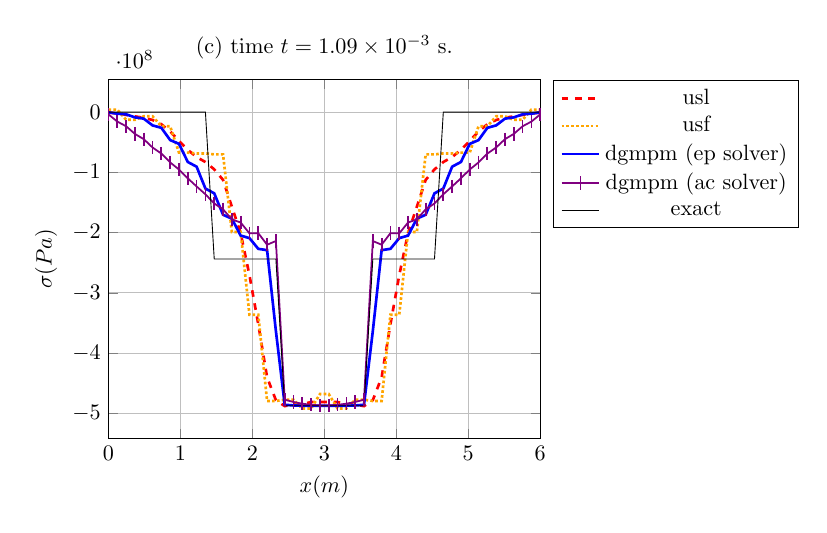
\begin{tikzpicture}[scale=0.8]
\begin{axis}[xlabel=$x (m)$,ylabel=$\sigma (Pa)$,ymajorgrids=true,xmajorgrids=true,legend pos=outer north east,title={(c) time $t = 1.09\times 10^{-3} $ s.},xmin=0.,xmax=6.]
\addplot[Red,very thick,mark=none,dashed,mark size=3pt] coordinates {(0.0,-679166.0601331755) (0.12244897959183673,-2368189.594188208) (0.24489795918367346,-4606456.556212341) (0.36734693877551017,-6961578.395676694) (0.4897959183673469,-9332760.287028607) (0.6122448979591837,-12938682.464591796) (0.7346938775510203,-20102821.471402142) (0.8571428571428571,-32015823.341737133) (0.9795918367346939,-47676454.15860757) (1.1020408163265305,-62502940.42234602) (1.2244897959183674,-74544680.06037714) (1.346938775510204,-82775603.38522142) (1.4693877551020407,-94947363.4179823) (1.5918367346938775,-112415785.44002911) (1.7142857142857142,-156774491.63523546) (1.836734693877551,-200654618.50473383) (1.9591836734693877,-270646588.3413816) (2.0816326530612246,-351928629.9311485) (2.204081632653061,-440064160.15512294) (2.326530612244898,-477934424.91056436) (2.4489795918367347,-487815276.0764712) (2.571428571428571,-485351241.33413374) (2.693877551020408,-484406188.97201383) (2.816326530612245,-481035531.7602433) (2.9387755102040813,-481038509.8228564) (3.061224489795918,-481038509.8228558) (3.183673469387755,-481035531.7602443) (3.306122448979592,-484406188.9720135) (3.4285714285714284,-485351241.3341341) (3.5510204081632653,-487815276.07647014) (3.673469387755102,-477934424.9105651) (3.7959183673469385,-440064160.15512156) (3.9183673469387754,-351928629.931148) (4.040816326530612,-270646588.34138024) (4.163265306122449,-200654618.50473374) (4.285714285714286,-156774491.63523474) (4.408163265306122,-112415785.44002907) (4.530612244897959,-94947363.41798277) (4.653061224489796,-82775603.38522187) (4.775510204081632,-74544680.06037733) (4.8979591836734695,-62502940.42234604) (5.020408163265306,-47676454.158607304) (5.142857142857142,-32015823.341736842) (5.26530612244898,-20102821.471402) (5.387755102040816,-12938682.46459166) (5.5102040816326525,-9332760.287028512) (5.63265306122449,-6961578.395676572) (5.755102040816326,-4606456.55621225) (5.877551020408163,-2368189.594188123) (6.0,-679166.0601331636) };
\addplot[Orange,very thick,mark=none,densely dotted,mark size=3pt] coordinates {(0.0,4236951.290463989) (0.12244897959183673,4236951.290460123) (0.24489795918367346,-12679253.938911917) (0.36734693877551017,-12679253.938916743) (0.4897959183673469,-6922591.558428046) (0.6122448979591837,-6922591.558431343) (0.7346938775510203,-23459809.182112668) (0.8571428571428571,-23459809.18211712) (0.9795918367346939,-67167151.83770859) (1.1020408163265305,-67167151.83771148) (1.2244897959183674,-68479697.03436251) (1.346938775510204,-68479697.03436783) (1.4693877551020407,-70089580.65292576) (1.5918367346938775,-70089580.65292576) (1.7142857142857142,-198942113.00187883) (1.836734693877551,-198942113.00187835) (1.9591836734693877,-336192669.59109914) (2.0816326530612246,-336192669.59109795) (2.204081632653061,-479279910.7951127) (2.326530612244898,-479279910.795111) (2.4489795918367347,-477181511.2029586) (2.571428571428571,-477181511.20295614) (2.693877551020408,-491728219.61058974) (2.816326530612245,-491728219.6105894) (2.9387755102040813,-467835686.5023686) (3.061224489795918,-467835686.50236756) (3.183673469387755,-491728219.6105915) (3.306122448979592,-491728219.61058766) (3.4285714285714284,-477181511.20295787) (3.5510204081632653,-477181511.20295686) (3.673469387755102,-479279910.79511243) (3.7959183673469385,-479279910.7951107) (3.9183673469387754,-336192669.5910962) (4.040816326530612,-336192669.59110004) (4.163265306122449,-198942113.0018753) (4.285714285714286,-198942113.00188202) (4.408163265306122,-70089580.65291941) (4.530612244897959,-70089580.65293229) (4.653061224489796,-68479697.03436142) (4.775510204081632,-68479697.03436944) (4.8979591836734695,-67167151.83770534) (5.020408163265306,-67167151.83771467) (5.142857142857142,-23459809.182109676) (5.26530612244898,-23459809.182119854) (5.387755102040816,-6922591.558424118) (5.5102040816326525,-6922591.558435734) (5.63265306122449,-12679253.938909372) (5.755102040816326,-12679253.938918298) (5.877551020408163,4236951.290467103) (6.0,4236951.290456754) };
\addplot[Blue,very thick,mark=none,solid,mark size=3pt] coordinates {(0.0,-298852.1952411225) (0.12244897959183673,-2592980.4740912793) (0.24489795918367346,-3560236.4322381816) (0.36734693877551017,-8652722.221047912) (0.4897959183673469,-10777216.673686886) (0.6122448979591837,-21974314.707157355) (0.7346938775510203,-26009924.918005344) (0.8571428571428571,-46347563.10657899) (0.9795918367346939,-52593345.171819046) (1.1020408163265305,-82683979.65035231) (1.2244897959183674,-90525380.97285904) (1.346938775510204,-126773557.44849168) (1.4693877551020407,-134743667.28836828) (1.5918367346938775,-170219249.4978279) (1.7142857142857142,-176744937.7749974) (1.836734693877551,-204799464.24688196) (1.9591836734693877,-209064122.25232974) (2.0816326530612246,-226820170.49378502) (2.204081632653061,-229011964.3130221) (2.326530612244898,-363270795.9137317) (2.4489795918367347,-485529213.90073514) (2.571428571428571,-486748760.1951447) (2.693877551020408,-487164866.56783277) (2.816326530612245,-487268871.16624963) (2.9387755102040813,-487285807.7274521) (3.061224489795918,-487285807.7274521) (3.183673469387755,-487268871.16624963) (3.306122448979592,-487164866.56783277) (3.4285714285714284,-486748760.1951447) (3.5510204081632653,-485529213.90073514) (3.673469387755102,-363270795.91372997) (3.7959183673469385,-229011964.3130223) (3.9183673469387754,-226820170.49378502) (4.040816326530612,-209064122.25232938) (4.163265306122449,-204799464.2468816) (4.285714285714286,-176744937.77499697) (4.408163265306122,-170219249.4978276) (4.530612244897959,-134743667.28836808) (4.653061224489796,-126773557.44849148) (4.775510204081632,-90525380.9728589) (4.8979591836734695,-82683979.65035222) (5.020408163265306,-52593345.171819076) (5.142857142857142,-46347563.10657902) (5.26530612244898,-26009924.918005634) (5.387755102040816,-21974314.707157686) (5.5102040816326525,-10777216.673687106) (5.63265306122449,-8652722.22104813) (5.755102040816326,-3560236.4322383474) (5.877551020408163,-2592980.4740913147) (6.0,-298852.1952412414) };
\addplot[Purple,thick,mark=|,solid,mark size=3pt] coordinates {(0.0,-3699822.6801933693) (0.12244897959183673,-15656690.657919873) (0.24489795918367346,-23395010.37401582) (0.36734693877551017,-36103443.51008522) (0.4897959183673469,-44799564.7059784) (0.6122448979591837,-58626001.393915564) (0.7346938775510203,-68743311.52420163) (0.8571428571428571,-83413570.25799192) (0.9795918367346939,-95210786.60876837) (1.1020408163265305,-109767206.98229863) (1.2244897959183674,-123307254.49744721) (1.346938775510204,-136286963.85824355) (1.4693877551020407,-151490220.183104) (1.5918367346938775,-161259604.24498996) (1.7142857142857142,-177973600.29101613) (1.836734693877551,-183108322.81917205) (1.9591836734693877,-201165134.12201387) (2.0816326530612246,-200760737.51095787) (2.204081632653061,-220004370.6130868) (2.326530612244898,-213836576.44044873) (2.4489795918367347,-477124042.8840971) (2.571428571428571,-480953140.1350389) (2.693877551020408,-483830928.1925999) (2.816326530612245,-485620834.2660387) (2.9387755102040813,-486699217.4934911) (3.061224489795918,-486699217.4934911) (3.183673469387755,-485620834.2660387) (3.306122448979592,-483830928.1925999) (3.4285714285714284,-480953140.1350389) (3.5510204081632653,-477124042.8840971) (3.673469387755102,-213836576.44044736) (3.7959183673469385,-220004370.6130868) (3.9183673469387754,-200760737.5109577) (4.040816326530612,-201165134.1220135) (4.163265306122449,-183108322.81917205) (4.285714285714286,-177973600.2910157) (4.408163265306122,-161259604.24498972) (4.530612244897959,-151490220.18310383) (4.653061224489796,-136286963.85824338) (4.775510204081632,-123307254.49744716) (4.8979591836734695,-109767206.98229855) (5.020408163265306,-95210786.6087684) (5.142857142857142,-83413570.25799206) (5.26530612244898,-68743311.52420157) (5.387755102040816,-58626001.393915735) (5.5102040816326525,-44799564.70597822) (5.63265306122449,-36103443.51008532) (5.755102040816326,-23395010.374015827) (5.877551020408163,-15656690.657920003) (6.0,-3699822.6801932575) };
\addplot[black,thin,mark=none,solid,mark size=3pt] coordinates {(0.0,-0.0) (0.12244897959183673,-0.0) (0.24489795918367346,-0.0) (0.36734693877551017,-0.0) (0.4897959183673469,-0.0) (0.6122448979591837,-0.0) (0.7346938775510203,-0.0) (0.8571428571428571,-0.0) (0.9795918367346939,-0.0) (1.1020408163265305,-0.0) (1.2244897959183674,-0.0) (1.346938775510204,-0.0) (1.4693877551020407,-243643578.04719847) (1.5918367346938775,-243643578.04719847) (1.7142857142857142,-243643578.04719847) (1.836734693877551,-243643578.04719847) (1.9591836734693877,-243643578.04719847) (2.0816326530612246,-243643578.04719847) (2.204081632653061,-243643578.04719847) (2.326530612244898,-243643578.04719847) (2.4489795918367347,-487287156.09439695) (2.571428571428571,-487287156.09439695) (2.693877551020408,-487287156.09439695) (2.816326530612245,-487287156.09439695) (2.9387755102040813,-487287156.09439695) (3.061224489795918,-487287156.09439695) (3.183673469387755,-487287156.09439695) (3.306122448979592,-487287156.09439695) (3.4285714285714284,-487287156.09439695) (3.5510204081632653,-487287156.09439695) (3.673469387755102,-243643578.04719847) (3.7959183673469385,-243643578.04719847) (3.9183673469387754,-243643578.04719847) (4.040816326530612,-243643578.04719847) (4.163265306122449,-243643578.04719847) (4.285714285714286,-243643578.04719847) (4.408163265306122,-243643578.04719847) (4.530612244897959,-243643578.04719847) (4.653061224489796,-0.0) (4.775510204081632,-0.0) (4.8979591836734695,-0.0) (5.020408163265306,-0.0) (5.142857142857142,-0.0) (5.26530612244898,-0.0) (5.387755102040816,-0.0) (5.5102040816326525,-0.0) (5.63265306122449,-0.0) (5.755102040816326,-0.0) (5.877551020408163,-0.0) (6.0,-0.0) };
\legend{usl,usf,dgmpm (ep solver),dgmpm (ac solver),exact}
\end{axis}
\end{tikzpicture}
%%% Local Variables:
%%% mode: latex
%%% TeX-master: "../../mainManuscript"
%%% End:
}
  \caption{elastic-plastic RP stress}
  \label{fig:stress_elastoplastic_RP}
\end{figure}
\begin{figure}[h!]
  \centering
  {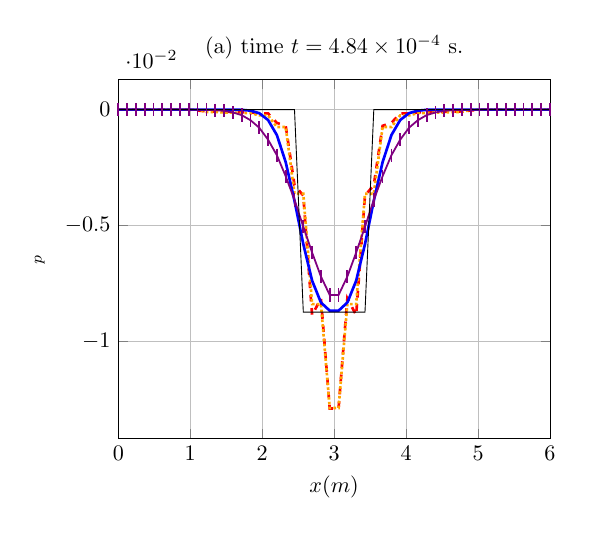
\begin{tikzpicture}[scale=0.8]
\begin{axis}[xlabel=$x (m)$,ylabel=$\eps^p$,ymajorgrids=true,xmajorgrids=true,legend pos=outer north east,title={(a) time $t = 4.84\times 10^{-4} $ s.},xmin=0.,xmax=6.]
\addplot[Red,very thick,mark=none,dashed,mark size=3pt] coordinates {(0.0,0.0) (0.12244897959183673,0.0) (0.24489795918367346,0.0) (0.36734693877551017,0.0) (0.4897959183673469,0.0) (0.6122448979591837,0.0) (0.7346938775510203,0.0) (0.8571428571428571,0.0) (0.9795918367346939,0.0) (1.1020408163265305,-3.791590211516079e-05) (1.2244897959183674,-7.70866275263142e-05) (1.346938775510204,-8.497586707829323e-05) (1.4693877551020407,-9.030872437715389e-05) (1.5918367346938775,-9.742060457186303e-05) (1.7142857142857142,-0.00011777294632526181) (1.836734693877551,-0.00011877997120884317) (1.9591836734693877,-0.00017229593911894644) (2.0816326530612246,-0.0001625095927714705) (2.204081632653061,-0.0005721718460187986) (2.326530612244898,-0.0006980928227095806) (2.4489795918367347,-0.003255684770391246) (2.571428571428571,-0.003703854150331533) (2.693877551020408,-0.008855536230217072) (2.816326530612245,-0.008134161982050364) (2.9387755102040813,-0.012877303196726952) (3.061224489795918,-0.012877303196726607) (3.183673469387755,-0.008134161982050527) (3.306122448979592,-0.008855536230216924) (3.4285714285714284,-0.00370385415033155) (3.5510204081632653,-0.0032556847703911866) (3.673469387755102,-0.0006980928227095723) (3.7959183673469385,-0.0005721718460187898) (3.9183673469387754,-0.0001625095927714674) (4.040816326530612,-0.00017229593911894956) (4.163265306122449,-0.00011877997120884148) (4.285714285714286,-0.00011777294632525957) (4.408163265306122,-9.74206045718636e-05) (4.530612244897959,-9.030872437715303e-05) (4.653061224489796,-8.497586707829776e-05) (4.775510204081632,-7.708662752631704e-05) (4.8979591836734695,-3.791590211516108e-05) (5.020408163265306,0.0) (5.142857142857142,0.0) (5.26530612244898,0.0) (5.387755102040816,0.0) (5.5102040816326525,0.0) (5.63265306122449,0.0) (5.755102040816326,0.0) (5.877551020408163,0.0) (6.0,0.0) };
\addplot[Orange,very thick,mark=none,densely dotted,mark size=3pt] coordinates {(0.0,0.0) (0.12244897959183673,0.0) (0.24489795918367346,0.0) (0.36734693877551017,0.0) (0.4897959183673469,0.0) (0.6122448979591837,0.0) (0.7346938775510203,0.0) (0.8571428571428571,0.0) (0.9795918367346939,0.0) (1.1020408163265305,0.0) (1.2244897959183674,-0.00010125340605535082) (1.346938775510204,-0.00010125340605535564) (1.4693877551020407,-0.00012349527304735526) (1.5918367346938775,-0.00012349527304735214) (1.7142857142857142,-0.0001510249264983643) (1.836734693877551,-0.0001510249264983569) (1.9591836734693877,-0.0002468617206963456) (2.0816326530612246,-0.00024686172069637857) (2.204081632653061,-0.0007504349417450695) (2.326530612244898,-0.0007504349417451243) (2.4489795918367347,-0.0036281593420660124) (2.571428571428571,-0.003628159342065948) (2.693877551020408,-0.008380076410022513) (2.816326530612245,-0.008380076410022256) (2.9387755102040813,-0.012853848358106693) (3.061224489795918,-0.0128538483581062) (3.183673469387755,-0.008380076410022525) (3.306122448979592,-0.008380076410022235) (3.4285714285714284,-0.003628159342066054) (3.5510204081632653,-0.00362815934206591) (3.673469387755102,-0.000750434941745111) (3.7959183673469385,-0.0007504349417450832) (3.9183673469387754,-0.00024686172069633743) (4.040816326530612,-0.00024686172069637695) (4.163265306122449,-0.00015102492649834897) (4.285714285714286,-0.0001510249264983674) (4.408163265306122,-0.00012349527304735949) (4.530612244897959,-0.00012349527304735412) (4.653061224489796,-0.00010125340605534598) (4.775510204081632,-0.00010125340605535762) (4.8979591836734695,0.0) (5.020408163265306,0.0) (5.142857142857142,0.0) (5.26530612244898,0.0) (5.387755102040816,0.0) (5.5102040816326525,0.0) (5.63265306122449,0.0) (5.755102040816326,0.0) (5.877551020408163,0.0) (6.0,0.0) };
\addplot[Blue,very thick,mark=none,solid,mark size=3pt] coordinates {(0.0,0.0) (0.12244897959183673,0.0) (0.24489795918367346,0.0) (0.36734693877551017,0.0) (0.4897959183673469,0.0) (0.6122448979591837,-5.222502208891369e-16) (0.7346938775510203,-3.801924841744559e-14) (0.8571428571428571,-1.3141666139875138e-12) (0.9795918367346939,-2.8745591924304055e-11) (1.1020408163265305,-4.464150179000128e-10) (1.2244897959183674,-5.23467841943105e-09) (1.346938775510204,-4.812046858639944e-08) (1.4693877551020407,-3.554036475964955e-07) (1.5918367346938775,-2.1443096765697003e-06) (1.7142857142857142,-1.0689498023182154e-05) (1.836734693877551,-4.436466051051049e-05) (1.9591836734693877,-0.00015404085928397946) (2.0816326530612246,-0.00044873332231471766) (2.204081632653061,-0.0010984305872627827) (2.326530612244898,-0.0022622254025038953) (2.4489795918367347,-0.003929978610103271) (2.571428571428571,-0.005797119893456445) (2.693877551020408,-0.007371043418348148) (2.816326530612245,-0.008310826779347521) (2.9387755102040813,-0.00866523151909913) (3.061224489795918,-0.008665231519099129) (3.183673469387755,-0.008310826779347523) (3.306122448979592,-0.007371043418348151) (3.4285714285714284,-0.0057971198934564485) (3.5510204081632653,-0.003929978610103277) (3.673469387755102,-0.002262225402503906) (3.7959183673469385,-0.0010984305872627934) (3.9183673469387754,-0.0004487333223147267) (4.040816326530612,-0.00015404085928398656) (4.163265306122449,-4.4364660510512195e-05) (4.285714285714286,-1.0689498023171936e-05) (4.408163265306122,-2.144309676557212e-06) (4.530612244897959,-3.554036475865614e-07) (4.653061224489796,-4.8120468574194675e-08) (4.775510204081632,-5.234678408361617e-09) (4.8979591836734695,-4.4641501165571666e-10) (5.020408163265306,-2.874559277579898e-11) (5.142857142857142,-1.314168884640648e-12) (5.26530612244898,-3.802009991237095e-14) (5.387755102040816,-5.242370423816499e-16) (5.5102040816326525,0.0) (5.63265306122449,0.0) (5.755102040816326,0.0) (5.877551020408163,0.0) (6.0,0.0) };
\addplot[Purple,thick,mark=|,solid,mark size=3pt] coordinates {(0.0,0.0) (0.12244897959183673,0.0) (0.24489795918367346,0.0) (0.36734693877551017,0.0) (0.4897959183673469,0.0) (0.6122448979591837,-8.792960346028919e-09) (0.7346938775510203,-3.786059785712333e-08) (0.8571428571428571,-2.508230825960636e-07) (0.9795918367346939,-8.265800991640205e-07) (1.1020408163265305,-3.1496141333668006e-06) (1.2244897959183674,-8.446763423661959e-06) (1.346938775510204,-2.3732282649803162e-05) (1.4693877551020407,-5.37012668957574e-05) (1.5918367346938775,-0.0001218346548242481) (1.7142857142857142,-0.00023802460823782993) (1.836734693877551,-0.0004559513032346254) (1.9591836734693877,-0.0007809726729771441) (2.0816326530612246,-0.001295399844018457) (2.204081632653061,-0.0019660778146380876) (2.326530612244898,-0.0028685788119150535) (2.4489795918367347,-0.0038889012981570665) (2.571428571428571,-0.005047541335664232) (2.693877551020408,-0.006159956990320315) (2.816326530612245,-0.007191476068263296) (2.9387755102040813,-0.007990368709145173) (3.061224489795918,-0.007990368709145174) (3.183673469387755,-0.007191476068263297) (3.306122448979592,-0.0061599569903203226) (3.4285714285714284,-0.005047541335664235) (3.5510204081632653,-0.003888901298157069) (3.673469387755102,-0.0028685788119150574) (3.7959183673469385,-0.001966077814638091) (3.9183673469387754,-0.0012953998440184578) (4.040816326530612,-0.0007809726729771479) (4.163265306122449,-0.0004559513032346283) (4.285714285714286,-0.00023802460823782627) (4.408163265306122,-0.00012183465482424442) (4.530612244897959,-5.3701266895754845e-05) (4.653061224489796,-2.3732282649791524e-05) (4.775510204081632,-8.446763423651173e-06) (4.8979591836734695,-3.1496141333639622e-06) (5.020408163265306,-8.265800991657234e-07) (5.142857142857142,-2.5082308259663124e-07) (5.26530612244898,-3.786059785967782e-08) (5.387755102040816,-8.79296034631275e-09) (5.5102040816326525,0.0) (5.63265306122449,0.0) (5.755102040816326,0.0) (5.877551020408163,0.0) (6.0,0.0) };
\addplot[black,thin,mark=none,solid,mark size=3pt] coordinates {(0.0,-0.0) (0.12244897959183673,-0.0) (0.24489795918367346,-0.0) (0.36734693877551017,-0.0) (0.4897959183673469,-0.0) (0.6122448979591837,-0.0) (0.7346938775510203,-0.0) (0.8571428571428571,-0.0) (0.9795918367346939,-0.0) (1.1020408163265305,-0.0) (1.2244897959183674,-0.0) (1.346938775510204,-0.0) (1.4693877551020407,-0.0) (1.5918367346938775,-0.0) (1.7142857142857142,-0.0) (1.836734693877551,-0.0) (1.9591836734693877,-0.0) (2.0816326530612246,-0.0) (2.204081632653061,-0.0) (2.326530612244898,-0.0) (2.4489795918367347,-0.0) (2.571428571428571,-0.008728715609439695) (2.693877551020408,-0.008728715609439695) (2.816326530612245,-0.008728715609439695) (2.9387755102040813,-0.008728715609439695) (3.061224489795918,-0.008728715609439695) (3.183673469387755,-0.008728715609439695) (3.306122448979592,-0.008728715609439695) (3.4285714285714284,-0.008728715609439695) (3.5510204081632653,-0.0) (3.673469387755102,-0.0) (3.7959183673469385,-0.0) (3.9183673469387754,-0.0) (4.040816326530612,-0.0) (4.163265306122449,-0.0) (4.285714285714286,-0.0) (4.408163265306122,-0.0) (4.530612244897959,-0.0) (4.653061224489796,-0.0) (4.775510204081632,-0.0) (4.8979591836734695,-0.0) (5.020408163265306,-0.0) (5.142857142857142,-0.0) (5.26530612244898,-0.0) (5.387755102040816,-0.0) (5.5102040816326525,-0.0) (5.63265306122449,-0.0) (5.755102040816326,-0.0) (5.877551020408163,-0.0) (6.0,-0.0) };
%\legend{usl,usf,dgmpm (ep solver),dgmpm (ac solver),exact}
\end{axis}
\end{tikzpicture}
%%% Local Variables:
%%% mode: latex
%%% TeX-master: "../../mainManuscript"
%%% End:
}
  {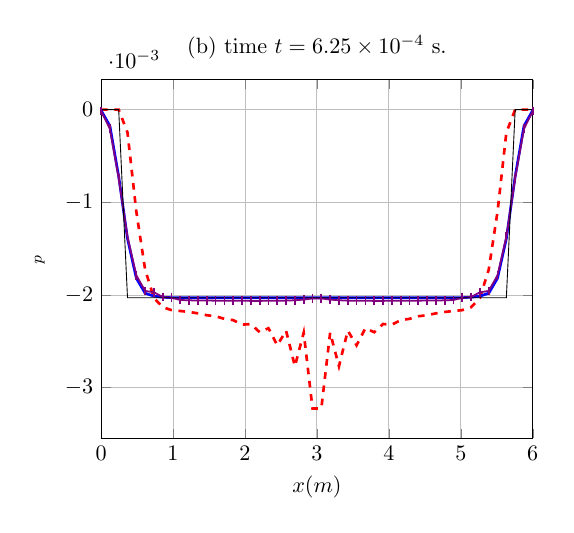
\begin{tikzpicture}[scale=0.8]
\begin{axis}[xlabel=$x (m)$,ylabel=$\eps^p$,ymajorgrids=true,xmajorgrids=true,legend pos=outer north east,title={(b) time $t = 6.25\times 10^{-4} $ s.},xmin=0.,xmax=6.]
\addplot[Red,very thick,mark=none,dashed] coordinates {(0.0,0.0) (0.12244897959183673,0.0) (0.24489795918367346,0.0) (0.36734693877551017,-0.0002478348228815541) (0.4897959183673469,-0.0011004378155012712) (0.6122448979591837,-0.0017260409269248597) (0.7346938775510203,-0.002031865332982762) (0.8571428571428571,-0.002132968518977378) (0.9795918367346939,-0.0021636018350532395) (1.1020408163265305,-0.0021733079916121177) (1.2244897959183674,-0.00218350748748031) (1.346938775510204,-0.002198645448466017) (1.4693877551020407,-0.002218920213241705) (1.5918367346938775,-0.002229697455331896) (1.7142857142857142,-0.002258121963594508) (1.836734693877551,-0.002271799079674154) (1.9591836734693877,-0.002320613632318322) (2.0816326530612246,-0.002313868472160546) (2.204081632653061,-0.0024020122032007017) (2.326530612244898,-0.0023588630990294623) (2.4489795918367347,-0.0025433455597807667) (2.571428571428571,-0.002385435935351422) (2.693877551020408,-0.0027693350417516906) (2.816326530612245,-0.0024065265204776445) (2.9387755102040813,-0.0032250612006492966) (3.061224489795918,-0.0032250612006492524) (3.183673469387755,-0.002406526520477666) (3.306122448979592,-0.0027693350417516823) (3.4285714285714284,-0.0023854359353514295) (3.5510204081632653,-0.0025433455597807628) (3.673469387755102,-0.002358863099029464) (3.7959183673469385,-0.0024020122032006983) (3.9183673469387754,-0.0023138684721605448) (4.040816326530612,-0.002320613632318319) (4.163265306122449,-0.0022717990796741546) (4.285714285714286,-0.0022581219635945077) (4.408163265306122,-0.0022296974553318956) (4.530612244897959,-0.0022189202132417056) (4.653061224489796,-0.0021986454484660173) (4.775510204081632,-0.0021835074874803095) (4.8979591836734695,-0.0021733079916121186) (5.020408163265306,-0.0021636018350532395) (5.142857142857142,-0.002132968518977378) (5.26530612244898,-0.002031865332982763) (5.387755102040816,-0.0017260409269248577) (5.5102040816326525,-0.0011004378155012658) (5.63265306122449,-0.0002478348228815494) (5.755102040816326,0.0) (5.877551020408163,0.0) (6.0,0.0) };
\addplot[Blue,very thick,mark=none,solid] coordinates {(0.0,-8.02367288935203e-06) (0.12244897959183673,-0.00017614426387335805) (0.24489795918367346,-0.0007207542691858686) (0.36734693877551017,-0.0013919930410856215) (0.4897959183673469,-0.001818355598439618) (0.6122448979591837,-0.001981300761387861) (0.7346938775510203,-0.0020125975551096974) (0.8571428571428571,-0.002024874952136019) (0.9795918367346939,-0.0020290867696967987) (1.1020408163265305,-0.002030353909504423) (1.2244897959183674,-0.0020306887880741907) (1.346938775510204,-0.0020307665725143873) (1.4693877551020407,-0.0020307824435747243) (1.5918367346938775,-0.0020307852835259937) (1.7142857142857142,-0.0020307857279245408) (1.836734693877551,-0.0020307857884822454) (1.9591836734693877,-0.00203078579562695) (2.0816326530612246,-0.002030785796351117) (2.204081632653061,-0.0020307857964135248) (2.326530612244898,-0.002030785796418031) (2.4489795918367347,-0.002030785796418302) (2.571428571428571,-0.0020307857964183135) (2.693877551020408,-0.002030785796418313) (2.816326530612245,-0.002030785796418313) (2.9387755102040813,-0.002030785796418314) (3.061224489795918,-0.0020307857964183135) (3.183673469387755,-0.0020307857964183135) (3.306122448979592,-0.0020307857964183126) (3.4285714285714284,-0.0020307857964183113) (3.5510204081632653,-0.0020307857964183005) (3.673469387755102,-0.002030785796418031) (3.7959183673469385,-0.0020307857964135217) (3.9183673469387754,-0.0020307857963511138) (4.040816326530612,-0.002030785795626948) (4.163265306122449,-0.0020307857884822433) (4.285714285714286,-0.0020307857279245403) (4.408163265306122,-0.0020307852835259915) (4.530612244897959,-0.0020307824435747226) (4.653061224489796,-0.0020307665725143842) (4.775510204081632,-0.002030688788074188) (4.8979591836734695,-0.0020303539095044196) (5.020408163265306,-0.0020290867696967953) (5.142857142857142,-0.0020248749521360144) (5.26530612244898,-0.0020125975551096966) (5.387755102040816,-0.0019813007613878565) (5.5102040816326525,-0.0018183555984396154) (5.63265306122449,-0.0013919930410856195) (5.755102040816326,-0.0007207542691858678) (5.877551020408163,-0.0001761442638733595) (6.0,-8.023672889353243e-06) };
\addplot[Purple,thick,mark=|,solid] coordinates {(0.0,-1.4376766038990375e-05) (0.12244897959183673,-0.0002078915703532438) (0.24489795918367346,-0.000740641579521879) (0.36734693877551017,-0.0013729886129224668) (0.4897959183673469,-0.001786873759629078) (0.6122448979591837,-0.0019568221398810824) (0.7346938775510203,-0.0019710253863315036) (0.8571428571428571,-0.002021925787657269) (0.9795918367346939,-0.00203043998544926) (1.1020408163265305,-0.002054595482920735) (1.2244897959183674,-0.0020576351166755064) (1.346938775510204,-0.0020609998518549564) (1.4693877551020407,-0.0020606031772355433) (1.5918367346938775,-0.002061501114574304) (1.7142857142857142,-0.002061887903336271) (1.836734693877551,-0.002062455598454706) (1.9591836734693877,-0.0020617923316583004) (2.0816326530612246,-0.002064203896841495) (2.204081632653061,-0.0020644266901542695) (2.326530612244898,-0.0020621094945296272) (2.4489795918367347,-0.002062767607181189) (2.571428571428571,-0.002061489252343496) (2.693877551020408,-0.0020573197208032658) (2.816326530612245,-0.0020502799029179) (2.9387755102040813,-0.0020377776694292327) (3.061224489795918,-0.0020377776694292327) (3.183673469387755,-0.002050279902917899) (3.306122448979592,-0.002057319720803265) (3.4285714285714284,-0.0020614892523434956) (3.5510204081632653,-0.0020627676071811878) (3.673469387755102,-0.0020621094945296285) (3.7959183673469385,-0.0020644266901542695) (3.9183673469387754,-0.0020642038968414953) (4.040816326530612,-0.0020617923316583004) (4.163265306122449,-0.002062455598454705) (4.285714285714286,-0.0020618879033362705) (4.408163265306122,-0.002061501114574307) (4.530612244897959,-0.0020606031772355464) (4.653061224489796,-0.002060999851854956) (4.775510204081632,-0.002057635116675507) (4.8979591836734695,-0.002054595482920736) (5.020408163265306,-0.002030439985449261) (5.142857142857142,-0.0020219257876572696) (5.26530612244898,-0.001971025386331503) (5.387755102040816,-0.0019568221398810802) (5.5102040816326525,-0.0017868737596290767) (5.63265306122449,-0.0013729886129224679) (5.755102040816326,-0.0007406415795218811) (5.877551020408163,-0.00020789157035324622) (6.0,-1.4376766038991588e-05) };
\addplot[black,thin,mark=none,solid] coordinates {(0.0,-0.0) (0.12244897959183673,-0.0) (0.24489795918367346,-0.0) (0.36734693877551017,-0.002030785796418313) (0.4897959183673469,-0.002030785796418313) (0.6122448979591837,-0.002030785796418313) (0.7346938775510203,-0.002030785796418313) (0.8571428571428571,-0.002030785796418313) (0.9795918367346939,-0.002030785796418313) (1.1020408163265305,-0.002030785796418313) (1.2244897959183674,-0.002030785796418313) (1.346938775510204,-0.002030785796418313) (1.4693877551020407,-0.002030785796418313) (1.5918367346938775,-0.002030785796418313) (1.7142857142857142,-0.002030785796418313) (1.836734693877551,-0.002030785796418313) (1.9591836734693877,-0.002030785796418313) (2.0816326530612246,-0.002030785796418313) (2.204081632653061,-0.002030785796418313) (2.326530612244898,-0.002030785796418313) (2.4489795918367347,-0.002030785796418313) (2.571428571428571,-0.002030785796418313) (2.693877551020408,-0.002030785796418313) (2.816326530612245,-0.002030785796418313) (2.9387755102040813,-0.002030785796418313) (3.061224489795918,-0.002030785796418313) (3.183673469387755,-0.002030785796418313) (3.306122448979592,-0.002030785796418313) (3.4285714285714284,-0.002030785796418313) (3.5510204081632653,-0.002030785796418313) (3.673469387755102,-0.002030785796418313) (3.7959183673469385,-0.002030785796418313) (3.9183673469387754,-0.002030785796418313) (4.040816326530612,-0.002030785796418313) (4.163265306122449,-0.002030785796418313) (4.285714285714286,-0.002030785796418313) (4.408163265306122,-0.002030785796418313) (4.530612244897959,-0.002030785796418313) (4.653061224489796,-0.002030785796418313) (4.775510204081632,-0.002030785796418313) (4.8979591836734695,-0.002030785796418313) (5.020408163265306,-0.002030785796418313) (5.142857142857142,-0.002030785796418313) (5.26530612244898,-0.002030785796418313) (5.387755102040816,-0.002030785796418313) (5.5102040816326525,-0.002030785796418313) (5.63265306122449,-0.002030785796418313) (5.755102040816326,-0.0) (5.877551020408163,-0.0) (6.0,-0.0) };
%\legend{usl 1ppc,dgmpm 1ppc (ep solver),dgmpm 1ppc (ac solver),exact}
\end{axis}
\end{tikzpicture}
%%% Local Variables:
%%% mode: latex
%%% TeX-master: "../../mainManuscript"
%%% End:
}
  {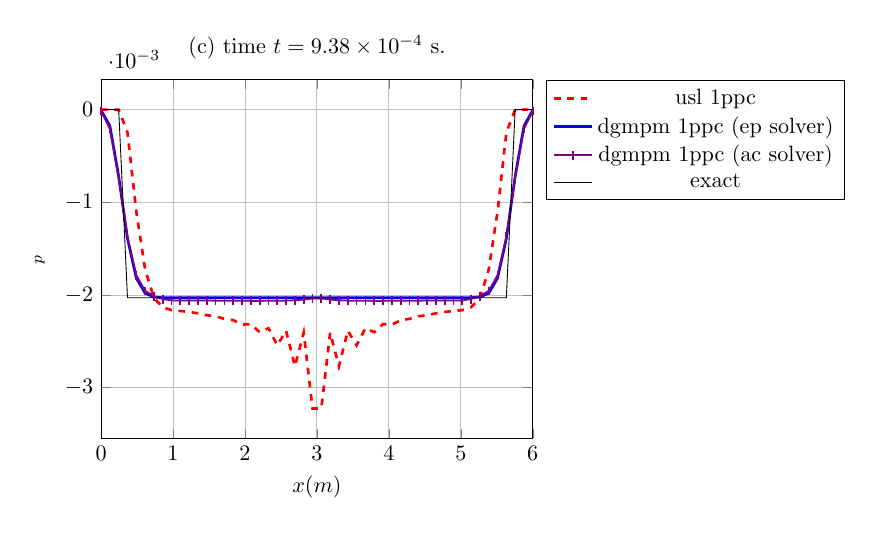
\begin{tikzpicture}[scale=0.8]
\begin{axis}[xlabel=$x (m)$,ylabel=$\eps^p$,ymajorgrids=true,xmajorgrids=true,legend pos=outer north east,title={(c) time $t = 9.38\times 10^{-4} $ s.},xmin=0.,xmax=6.]
\addplot[Red,very thick,mark=none,dashed] coordinates {(0.0,0.0) (0.12244897959183673,0.0) (0.24489795918367346,0.0) (0.36734693877551017,-0.0002478348228815541) (0.4897959183673469,-0.0011004378155012712) (0.6122448979591837,-0.0017260409269248597) (0.7346938775510203,-0.002031865332982762) (0.8571428571428571,-0.002132968518977378) (0.9795918367346939,-0.0021636018350532395) (1.1020408163265305,-0.0021733079916121177) (1.2244897959183674,-0.00218350748748031) (1.346938775510204,-0.002198645448466017) (1.4693877551020407,-0.002218920213241705) (1.5918367346938775,-0.002229697455331896) (1.7142857142857142,-0.002258121963594508) (1.836734693877551,-0.002271799079674154) (1.9591836734693877,-0.002320613632318322) (2.0816326530612246,-0.002313868472160546) (2.204081632653061,-0.0024020122032007017) (2.326530612244898,-0.0023588630990294623) (2.4489795918367347,-0.0025433455597807667) (2.571428571428571,-0.002385435935351422) (2.693877551020408,-0.0027693350417516906) (2.816326530612245,-0.0024065265204776445) (2.9387755102040813,-0.0032250612006492966) (3.061224489795918,-0.0032250612006492524) (3.183673469387755,-0.002406526520477666) (3.306122448979592,-0.0027693350417516823) (3.4285714285714284,-0.0023854359353514295) (3.5510204081632653,-0.0025433455597807628) (3.673469387755102,-0.002358863099029464) (3.7959183673469385,-0.0024020122032006983) (3.9183673469387754,-0.0023138684721605448) (4.040816326530612,-0.002320613632318319) (4.163265306122449,-0.0022717990796741546) (4.285714285714286,-0.0022581219635945077) (4.408163265306122,-0.0022296974553318956) (4.530612244897959,-0.0022189202132417056) (4.653061224489796,-0.0021986454484660173) (4.775510204081632,-0.0021835074874803095) (4.8979591836734695,-0.0021733079916121186) (5.020408163265306,-0.0021636018350532395) (5.142857142857142,-0.002132968518977378) (5.26530612244898,-0.002031865332982763) (5.387755102040816,-0.0017260409269248577) (5.5102040816326525,-0.0011004378155012658) (5.63265306122449,-0.0002478348228815494) (5.755102040816326,0.0) (5.877551020408163,0.0) (6.0,0.0) };
\addplot[Blue,very thick,mark=none,solid] coordinates {(0.0,-8.02367288935203e-06) (0.12244897959183673,-0.00017614426387335805) (0.24489795918367346,-0.0007207542691858686) (0.36734693877551017,-0.0013919930410856215) (0.4897959183673469,-0.001818355598439618) (0.6122448979591837,-0.001981300761387861) (0.7346938775510203,-0.0020224370921330336) (0.8571428571428571,-0.0020297345877472663) (0.9795918367346939,-0.0020306845407067867) (1.1020408163265305,-0.0020307781868908383) (1.2244897959183674,-0.002030785343345076) (1.346938775510204,-0.0020307857747949186) (1.4693877551020407,-0.002030785795584013) (1.5918367346938775,-0.0020307857963921434) (1.7142857142857142,-0.002030785796417646) (1.836734693877551,-0.0020307857964183005) (1.9591836734693877,-0.0020307857964183143) (2.0816326530612246,-0.002030785796418315) (2.204081632653061,-0.0020307857964183143) (2.326530612244898,-0.0020307857964183143) (2.4489795918367347,-0.002030785796418315) (2.571428571428571,-0.002030785796418316) (2.693877551020408,-0.0020307857964183143) (2.816326530612245,-0.0020307857964183143) (2.9387755102040813,-0.0020307857964183143) (3.061224489795918,-0.0020307857964183143) (3.183673469387755,-0.0020307857964183143) (3.306122448979592,-0.002030785796418315) (3.4285714285714284,-0.0020307857964183143) (3.5510204081632653,-0.002030785796418313) (3.673469387755102,-0.0020307857964183126) (3.7959183673469385,-0.0020307857964183126) (3.9183673469387754,-0.0020307857964183135) (4.040816326530612,-0.0020307857964183126) (4.163265306122449,-0.002030785796418296) (4.285714285714286,-0.002030785796417643) (4.408163265306122,-0.002030785796392141) (4.530612244897959,-0.002030785795584008) (4.653061224489796,-0.0020307857747949147) (4.775510204081632,-0.002030785343345074) (4.8979591836734695,-0.0020307781868908327) (5.020408163265306,-0.002030684540706785) (5.142857142857142,-0.0020297345877472632) (5.26530612244898,-0.0020224370921330275) (5.387755102040816,-0.0019813007613878565) (5.5102040816326525,-0.0018183555984396154) (5.63265306122449,-0.0013919930410856195) (5.755102040816326,-0.0007207542691858678) (5.877551020408163,-0.0001761442638733595) (6.0,-8.023672889353243e-06) };
\addplot[Purple,thick,mark=|,solid] coordinates {(0.0,-1.4376766038990375e-05) (0.12244897959183673,-0.0002078915703532438) (0.24489795918367346,-0.000740641579521879) (0.36734693877551017,-0.0013729886129224668) (0.4897959183673469,-0.001786873759629078) (0.6122448979591837,-0.0019568221398810824) (0.7346938775510203,-0.002012310558600745) (0.8571428571428571,-0.002044949844264105) (0.9795918367346939,-0.002058346964042081) (1.1020408163265305,-0.0020602219089299787) (1.2244897959183674,-0.0020610958163181556) (1.346938775510204,-0.0020609998518549564) (1.4693877551020407,-0.0020606031772355433) (1.5918367346938775,-0.002061501114574304) (1.7142857142857142,-0.002061887903336271) (1.836734693877551,-0.002062455598454706) (1.9591836734693877,-0.0020617923316583004) (2.0816326530612246,-0.002064203896841495) (2.204081632653061,-0.0020644266901542695) (2.326530612244898,-0.0020621094945296272) (2.4489795918367347,-0.002062767607181189) (2.571428571428571,-0.002061489252343496) (2.693877551020408,-0.0020573197208032658) (2.816326530612245,-0.0020502799029179) (2.9387755102040813,-0.0020377776694292327) (3.061224489795918,-0.0020377776694292327) (3.183673469387755,-0.002050279902917899) (3.306122448979592,-0.002057319720803265) (3.4285714285714284,-0.0020614892523434956) (3.5510204081632653,-0.0020627676071811878) (3.673469387755102,-0.0020621094945296285) (3.7959183673469385,-0.0020644266901542695) (3.9183673469387754,-0.0020642038968414953) (4.040816326530612,-0.0020617923316583004) (4.163265306122449,-0.002062455598454705) (4.285714285714286,-0.0020618879033362705) (4.408163265306122,-0.002061501114574307) (4.530612244897959,-0.0020606031772355464) (4.653061224489796,-0.002060999851854956) (4.775510204081632,-0.0020610958163181543) (4.8979591836734695,-0.002060221908929976) (5.020408163265306,-0.0020583469640420783) (5.142857142857142,-0.0020449498442641056) (5.26530612244898,-0.0020123105586007457) (5.387755102040816,-0.0019568221398810802) (5.5102040816326525,-0.0017868737596290767) (5.63265306122449,-0.0013729886129224679) (5.755102040816326,-0.0007406415795218811) (5.877551020408163,-0.00020789157035324622) (6.0,-1.4376766038991588e-05) };
\addplot[black,thin,mark=none,solid] coordinates {(0.0,-0.0) (0.12244897959183673,-0.0) (0.24489795918367346,-0.0) (0.36734693877551017,-0.002030785796418313) (0.4897959183673469,-0.002030785796418313) (0.6122448979591837,-0.002030785796418313) (0.7346938775510203,-0.002030785796418313) (0.8571428571428571,-0.002030785796418313) (0.9795918367346939,-0.002030785796418313) (1.1020408163265305,-0.002030785796418313) (1.2244897959183674,-0.002030785796418313) (1.346938775510204,-0.002030785796418313) (1.4693877551020407,-0.002030785796418313) (1.5918367346938775,-0.002030785796418313) (1.7142857142857142,-0.002030785796418313) (1.836734693877551,-0.002030785796418313) (1.9591836734693877,-0.002030785796418313) (2.0816326530612246,-0.002030785796418313) (2.204081632653061,-0.002030785796418313) (2.326530612244898,-0.002030785796418313) (2.4489795918367347,-0.002030785796418313) (2.571428571428571,-0.002030785796418313) (2.693877551020408,-0.002030785796418313) (2.816326530612245,-0.002030785796418313) (2.9387755102040813,-0.002030785796418313) (3.061224489795918,-0.002030785796418313) (3.183673469387755,-0.002030785796418313) (3.306122448979592,-0.002030785796418313) (3.4285714285714284,-0.002030785796418313) (3.5510204081632653,-0.002030785796418313) (3.673469387755102,-0.002030785796418313) (3.7959183673469385,-0.002030785796418313) (3.9183673469387754,-0.002030785796418313) (4.040816326530612,-0.002030785796418313) (4.163265306122449,-0.002030785796418313) (4.285714285714286,-0.002030785796418313) (4.408163265306122,-0.002030785796418313) (4.530612244897959,-0.002030785796418313) (4.653061224489796,-0.002030785796418313) (4.775510204081632,-0.002030785796418313) (4.8979591836734695,-0.002030785796418313) (5.020408163265306,-0.002030785796418313) (5.142857142857142,-0.002030785796418313) (5.26530612244898,-0.002030785796418313) (5.387755102040816,-0.002030785796418313) (5.5102040816326525,-0.002030785796418313) (5.63265306122449,-0.002030785796418313) (5.755102040816326,-0.0) (5.877551020408163,-0.0) (6.0,-0.0) };
\legend{usl 1ppc,dgmpm 1ppc (ep solver),dgmpm 1ppc (ac solver),exact}
\end{axis}
\end{tikzpicture}
%%% Local Variables:
%%% mode: latex
%%% TeX-master: "../../mainManuscript"
%%% End:
}
  \caption{elastic-plastic RP epsp}
  \label{fig:epsp_elastoplastic_RP}
\end{figure}
\begin{figure}[h!]
  \centering
  {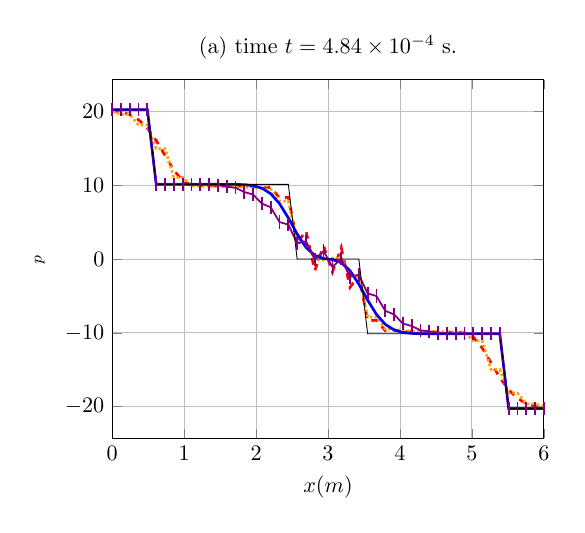
\begin{tikzpicture}[scale=0.8]
\begin{axis}[xlabel=$x (m)$,ylabel=$\eps^p$,ymajorgrids=true,xmajorgrids=true,legend pos=outer north east,title={(a) time $t = 4.84\times 10^{-4} $ s.},xmin=0.,xmax=6.]
\addplot[Red,very thick,mark=none,dashed,mark size=3pt] coordinates {(0.0,20.097963912667037) (0.12244897959183673,19.948200686683876) (0.24489795918367346,19.581623512332886) (0.36734693877551017,18.880401887543975) (0.4897959183673469,17.722027378885375) (0.6122448979591837,16.06462148503811) (0.7346938775510203,14.04922210395701) (0.8571428571428571,12.050777140391757) (0.9795918367346939,10.594448884991046) (1.1020408163265305,10.000299710369095) (1.2244897959183674,9.921016971597252) (1.346938775510204,9.905209334686656) (1.4693877551020407,9.897486036553882) (1.5918367346938775,9.881252793533395) (1.7142857142857142,9.874006895319209) (1.836734693877551,9.827852089496398) (1.9591836734693877,9.84660741015339) (2.0816326530612246,9.635377249359347) (2.204081632653061,9.703660809593103) (2.326530612244898,8.285921376176095) (2.4489795918367347,8.370712342612837) (2.571428571428571,2.1722672846759363) (2.693877551020408,3.830651803002166) (2.816326530612245,-1.5782561078814068) (2.9387755102040813,1.7774061156194738) (3.061224489795918,-1.777406115619491) (3.183673469387755,1.578256107881407) (3.306122448979592,-3.830651803002178) (3.4285714285714284,-2.172267284675949) (3.5510204081632653,-8.370712342612856) (3.673469387755102,-8.285921376176088) (3.7959183673469385,-9.703660809593108) (3.9183673469387754,-9.63537724935935) (4.040816326530612,-9.846607410153386) (4.163265306122449,-9.827852089496393) (4.285714285714286,-9.874006895319202) (4.408163265306122,-9.881252793533392) (4.530612244897959,-9.897486036553879) (4.653061224489796,-9.905209334686653) (4.775510204081632,-9.921016971597266) (4.8979591836734695,-10.000299710369097) (5.020408163265306,-10.594448884991042) (5.142857142857142,-12.05077714039174) (5.26530612244898,-14.049222103957007) (5.387755102040816,-16.064621485038092) (5.5102040816326525,-17.722027378885365) (5.63265306122449,-18.880401887543975) (5.755102040816326,-19.58162351233289) (5.877551020408163,-19.94820068668387) (6.0,-20.09796391266704) };
\addplot[Orange,very thick,mark=none,densely dotted,mark size=3pt] coordinates {(0.0,19.98524356533391) (0.12244897959183673,19.624972673600908) (0.24489795918367346,19.62497267360088) (0.36734693877551017,18.160148281550097) (0.4897959183673469,18.160148281550075) (0.6122448979591837,14.967460990115796) (0.7346938775510203,14.967460990115748) (0.8571428571428571,11.093523181440727) (0.9795918367346939,11.093523181440661) (1.1020408163265305,9.884184161534229) (1.2244897959183674,9.88418416153415) (1.346938775510204,9.848988655347343) (1.4693877551020407,9.848988655347272) (1.5918367346938775,9.805312262992565) (1.7142857142857142,9.805312262992501) (1.836734693877551,9.73354264540347) (1.9591836734693877,9.733542645403414) (2.0816326530612246,9.471881937395924) (2.204081632653061,9.471881937395832) (2.326530612244898,7.860641714627962) (2.4489795918367347,7.860641714627863) (2.571428571428571,2.220437432310992) (2.693877551020408,2.220437432310934) (2.816326530612245,-0.12736436093351383) (2.9387755102040813,-0.1273643609335115) (3.061224489795918,0.12736436093352144) (3.183673469387755,0.12736436093350467) (3.306122448979592,-2.220437432310998) (3.4285714285714284,-2.220437432310941) (3.5510204081632653,-7.860641714628002) (3.673469387755102,-7.860641714627828) (3.7959183673469385,-9.47188193739596) (3.9183673469387754,-9.471881937395791) (4.040816326530612,-9.733542645403523) (4.163265306122449,-9.73354264540336) (4.285714285714286,-9.805312262992585) (4.408163265306122,-9.805312262992468) (4.530612244897959,-9.848988655347373) (4.653061224489796,-9.848988655347233) (4.775510204081632,-9.884184161534241) (4.8979591836734695,-9.884184161534145) (5.020408163265306,-11.093523181440743) (5.142857142857142,-11.093523181440638) (5.26530612244898,-14.967460990115821) (5.387755102040816,-14.967460990115727) (5.5102040816326525,-18.1601482815501) (5.63265306122449,-18.16014828155006) (5.755102040816326,-19.624972673600908) (5.877551020408163,-19.62497267360089) (6.0,-19.985243565333896) };
\addplot[Blue,very thick,mark=none,solid,mark size=3pt] coordinates {(0.0,20.254787341673307) (0.12244897959183673,20.254787341673307) (0.24489795918367346,20.254787341673303) (0.36734693877551017,20.254787341673307) (0.4897959183673469,20.254787341673307) (0.6122448979591837,10.127393670836044) (0.7346938775510203,10.127393670792543) (0.8571428571428571,10.127393669311907) (0.9795918367346939,10.12739363748491) (1.1020408163265305,10.127393152888688) (1.2244897959183674,10.127387597360176) (1.346938775510204,10.127337839606644) (1.4693877551020407,10.1269813177698) (1.5918367346938775,10.124905759760324) (1.7142857142857142,10.114991301522732) (1.836734693877551,10.07592007470102) (1.9591836734693877,9.948669504170498) (2.0816326530612246,9.606755903306565) (2.204081632653061,8.852951991780422) (2.326530612244898,7.502672205682327) (2.4489795918367347,5.567680388456237) (2.571428571428571,3.401350808977297) (2.693877551020408,1.5752238210466734) (2.816326530612245,0.4848507939028141) (2.9387755102040813,0.07365669858902443) (3.061224489795918,-0.07365669858903101) (3.183673469387755,-0.48485079390282165) (3.306122448979592,-1.5752238210466838) (3.4285714285714284,-3.401350808977308) (3.5510204081632653,-5.56768038845625) (3.673469387755102,-7.502672205682339) (3.7959183673469385,-8.852951991780442) (3.9183673469387754,-9.606755903306581) (4.040816326530612,-9.948669504170525) (4.163265306122449,-10.075920074701049) (4.285714285714286,-10.11499130152276) (4.408163265306122,-10.124905759760349) (4.530612244897959,-10.126981317769818) (4.653061224489796,-10.12733783960665) (4.775510204081632,-10.127387597360173) (4.8979591836734695,-10.127393152888683) (5.020408163265306,-10.127393637484907) (5.142857142857142,-10.127393669311903) (5.26530612244898,-10.127393670792548) (5.387755102040816,-10.12739367083605) (5.5102040816326525,-20.25478734167332) (5.63265306122449,-20.254787341673318) (5.755102040816326,-20.25478734167332) (5.877551020408163,-20.25478734167332) (6.0,-20.254787341673314) };
\addplot[Purple,thick,mark=|,solid,mark size=3pt] coordinates {(0.0,20.254787341673307) (0.12244897959183673,20.254787341673307) (0.24489795918367346,20.254787341673303) (0.36734693877551017,20.254787341673307) (0.4897959183673469,20.254787341673307) (0.6122448979591837,10.127346919706891) (0.7346938775510203,10.12727737257173) (0.8571428571428571,10.126334047747402) (0.9795918367346939,10.125114755347433) (1.1020408163265305,10.11630010371687) (1.2244897959183674,10.106478421888186) (1.346938775510204,10.055869021868029) (1.4693877551020407,10.008062509066779) (1.5918367346938775,9.808511707883639) (1.7142857142857142,9.65367054792998) (1.836734693877551,9.082103441085764) (1.9591836734693877,8.739386895433114) (2.0816326530612246,7.513279145883331) (2.204081632653061,7.01727886939908) (2.326530612244898,5.014678544229133) (2.4489795918367347,4.663359241304864) (2.571428571428571,2.1468259041555218) (2.693877551020408,2.417528079544121) (2.816326530612245,-0.05847419216266908) (2.9387755102040813,1.0746179516287027) (3.061224489795918,-1.0746179516287169) (3.183673469387755,0.058474192162660144) (3.306122448979592,-2.417528079544138) (3.4285714285714284,-2.1468259041555355) (3.5510204081632653,-4.663359241304882) (3.673469387755102,-5.014678544229146) (3.7959183673469385,-7.017278869399091) (3.9183673469387754,-7.513279145883345) (4.040816326530612,-8.739386895433125) (4.163265306122449,-9.082103441085776) (4.285714285714286,-9.65367054792999) (4.408163265306122,-9.808511707883648) (4.530612244897959,-10.008062509066782) (4.653061224489796,-10.055869021868036) (4.775510204081632,-10.10647842188818) (4.8979591836734695,-10.11630010371688) (5.020408163265306,-10.125114755347425) (5.142857142857142,-10.12633404774741) (5.26530612244898,-10.127277372571715) (5.387755102040816,-10.127346919706907) (5.5102040816326525,-20.25478734167332) (5.63265306122449,-20.254787341673318) (5.755102040816326,-20.25478734167332) (5.877551020408163,-20.25478734167332) (6.0,-20.254787341673314) };
\addplot[black,thin,mark=none,solid,mark size=3pt] coordinates {(0.0,20.25478734167333) (0.12244897959183673,20.25478734167333) (0.24489795918367346,20.25478734167333) (0.36734693877551017,20.25478734167333) (0.4897959183673469,20.25478734167333) (0.6122448979591837,10.127393670836666) (0.7346938775510203,10.127393670836666) (0.8571428571428571,10.127393670836666) (0.9795918367346939,10.127393670836666) (1.1020408163265305,10.127393670836666) (1.2244897959183674,10.127393670836666) (1.346938775510204,10.127393670836666) (1.4693877551020407,10.127393670836666) (1.5918367346938775,10.127393670836666) (1.7142857142857142,10.127393670836666) (1.836734693877551,10.127393670836666) (1.9591836734693877,10.127393670836666) (2.0816326530612246,10.127393670836666) (2.204081632653061,10.127393670836666) (2.326530612244898,10.127393670836666) (2.4489795918367347,10.127393670836666) (2.571428571428571,-0.0) (2.693877551020408,-0.0) (2.816326530612245,-0.0) (2.9387755102040813,-0.0) (3.061224489795918,-0.0) (3.183673469387755,-0.0) (3.306122448979592,-0.0) (3.4285714285714284,-0.0) (3.5510204081632653,-10.127393670836666) (3.673469387755102,-10.127393670836666) (3.7959183673469385,-10.127393670836666) (3.9183673469387754,-10.127393670836666) (4.040816326530612,-10.127393670836666) (4.163265306122449,-10.127393670836666) (4.285714285714286,-10.127393670836666) (4.408163265306122,-10.127393670836666) (4.530612244897959,-10.127393670836666) (4.653061224489796,-10.127393670836666) (4.775510204081632,-10.127393670836666) (4.8979591836734695,-10.127393670836666) (5.020408163265306,-10.127393670836666) (5.142857142857142,-10.127393670836666) (5.26530612244898,-10.127393670836666) (5.387755102040816,-10.127393670836666) (5.5102040816326525,-20.25478734167333) (5.63265306122449,-20.25478734167333) (5.755102040816326,-20.25478734167333) (5.877551020408163,-20.25478734167333) (6.0,-20.25478734167333) };
%\legend{usl,usf,dgmpm (ep solver),dgmpm (ac solver),exact}
\end{axis}
\end{tikzpicture}
%%% Local Variables:
%%% mode: latex
%%% TeX-master: "../../mainManuscript"
%%% End:
}
  {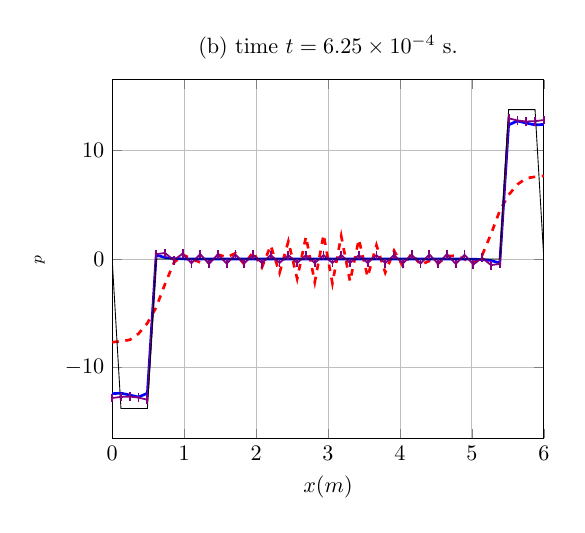
\begin{tikzpicture}[scale=0.8]
\begin{axis}[xlabel=$x (m)$,ylabel=$\eps^p$,ymajorgrids=true,xmajorgrids=true,legend pos=outer north east,title={(b) time $t = 6.25\times 10^{-4} $ s.},xmin=0.,xmax=6.]
\addplot[Red,very thick,mark=none,dashed] coordinates {(0.0,-7.656775715214294) (0.12244897959183673,-7.571339609307247) (0.24489795918367346,-7.438298117574187) (0.36734693877551017,-6.871029176921102) (0.4897959183673469,-5.903192627910385) (0.6122448979591837,-4.452057017543719) (0.7346938775510203,-2.3010481858807137) (0.8571428571428571,-0.3610443561643931) (0.9795918367346939,0.4188880742890505) (1.1020408163265305,0.01523876833598381) (1.2244897959183674,-0.3087249726610329) (1.346938775510204,-0.2682346195141458) (1.4693877551020407,0.41346894641452914) (1.5918367346938775,0.17204334381941044) (1.7142857142857142,0.5321881814826378) (1.836734693877551,-0.5074097815176064) (1.9591836734693877,0.6574508309639426) (2.0816326530612246,-0.7746969731901449) (2.204081632653061,1.2501366726613066) (2.326530612244898,-1.2807853076694733) (2.4489795918367347,1.631639383742251) (2.571428571428571,-1.8095691375383345) (2.693877551020408,2.0564749800644937) (2.816326530612245,-2.129190071354842) (2.9387755102040813,2.240060604992734) (3.061224489795918,-2.240060604992724) (3.183673469387755,2.1291900713548246) (3.306122448979592,-2.0564749800644746) (3.4285714285714284,1.809569137538315) (3.5510204081632653,-1.6316393837422516) (3.673469387755102,1.2807853076694653) (3.7959183673469385,-1.2501366726612742) (3.9183673469387754,0.7746969731901434) (4.040816326530612,-0.657450830963913) (4.163265306122449,0.5074097815175931) (4.285714285714286,-0.5321881814826224) (4.408163265306122,-0.17204334381940892) (4.530612244897959,-0.41346894641450627) (4.653061224489796,0.2682346195141527) (4.775510204081632,0.3087249726610414) (4.8979591836734695,-0.015238768335992692) (5.020408163265306,-0.4188880742890616) (5.142857142857142,0.3610443561643748) (5.26530612244898,2.3010481858807146) (5.387755102040816,4.452057017543711) (5.5102040816326525,5.90319262791038) (5.63265306122449,6.871029176921099) (5.755102040816326,7.4382981175741865) (5.877551020408163,7.571339609307248) (6.0,7.656775715214293) };
\addplot[Blue,very thick,mark=none,solid] coordinates {(0.0,-12.397952325377972) (0.12244897959183673,-12.346999574642966) (0.24489795918367346,-12.523092906128134) (0.36734693877551017,-12.71053547781855) (0.4897959183673469,-12.35049907311499) (0.6122448979591837,0.3722186738331613) (0.7346938775510203,0.1368090990556044) (0.8571428571428571,0.04446044382179651) (0.9795918367346939,0.012779812577704604) (1.1020408163265305,0.0032485856428356346) (1.2244897959183674,0.0007296815528062405) (1.346938775510204,0.00014459919089050038) (1.4693877551020407,2.5219563746036564e-05) (1.5918367346938775,3.857895635058131e-06) (1.7142857142857142,5.15199447901326e-07) (1.836734693877551,5.969388946802084e-08) (1.9591836734693877,5.952534698926585e-09) (2.0816326530612246,5.054662228331333e-10) (2.204081632653061,3.605726635043781e-11) (2.326530612244898,2.127654817367282e-12) (2.4489795918367347,1.1360160010621981e-13) (2.571428571428571,1.3411408617982763e-14) (2.693877551020408,1.66517088668301e-14) (2.816326530612245,5.526766510246074e-15) (2.9387755102040813,6.098792312826054e-15) (3.061224489795918,2.7682726724007426e-15) (3.183673469387755,7.175699018437728e-15) (3.306122448979592,-1.434813028923028e-14) (3.4285714285714284,-8.513769125527232e-15) (3.5510204081632653,-1.0095742773609699e-13) (3.673469387755102,-2.1199430888032018e-12) (3.7959183673469385,-3.6039619852103143e-11) (3.9183673469387754,-5.0545241703127e-10) (4.040816326530612,-5.9525221489037014e-09) (4.163265306122449,-5.969386814802888e-08) (4.285714285714286,-5.151994230605103e-07) (4.408163265306122,-3.8578956228878976e-06) (4.530612244897959,-2.5219563737562718e-05) (4.653061224489796,-0.00014459919087944834) (4.775510204081632,-0.0007296815527927886) (4.8979591836734695,-0.0032485856428289012) (5.020408163265306,-0.012779812577696097) (5.142857142857142,-0.04446044382178102) (5.26530612244898,-0.13680909905559333) (5.387755102040816,-0.3722186738331447) (5.5102040816326525,12.350499073115015) (5.63265306122449,12.71053547781857) (5.755102040816326,12.523092906128156) (5.877551020408163,12.346999574642979) (6.0,12.39795232537799) };
\addplot[Purple,thick,mark=|,solid] coordinates {(0.0,-12.795628373535159) (0.12244897959183673,-12.695543273778933) (0.24489795918367346,-12.666110940711564) (0.36734693877551017,-12.75241410003132) (0.4897959183673469,-12.960739789752774) (0.6122448979591837,0.44192323057668886) (0.7346938775510203,0.5605175207125453) (0.8571428571428571,-0.1118177278404644) (0.9795918367346939,0.49857571480888807) (1.1020408163265305,-0.3912177295445921) (1.2244897959183674,0.45869222504142426) (1.346938775510204,-0.4542184988816014) (1.4693877551020407,0.4392500135640788) (1.5918367346938775,-0.4268192827562814) (1.7142857142857142,0.4185270888397142) (1.836734693877551,-0.39693938041336063) (1.9591836734693877,0.398295251539175) (2.0816326530612246,-0.37211426798041747) (2.204081632653061,0.37593537352436907) (2.326530612244898,-0.3607380778681954) (2.4489795918367347,0.36132221537101705) (2.571428571428571,-0.3654682237983432) (2.693877551020408,0.35826901292698654) (2.816326530612245,-0.3691156051231741) (2.9387755102040813,0.36040411668068795) (3.061224489795918,-0.3604041166806867) (3.183673469387755,0.369115605123182) (3.306122448979592,-0.3582690129270081) (3.4285714285714284,0.36546822379836186) (3.5510204081632653,-0.3613222153709926) (3.673469387755102,0.3607380778681742) (3.7959183673469385,-0.37593537352436845) (3.9183673469387754,0.37211426798044456) (4.040816326530612,-0.3982952515391655) (4.163265306122449,0.3969393804133886) (4.285714285714286,-0.4185270888397233) (4.408163265306122,0.42681928275629366) (4.530612244897959,-0.43925001356404864) (4.653061224489796,0.45421849888160465) (4.775510204081632,-0.4586922250414254) (4.8979591836734695,0.3912177295446241) (5.020408163265306,-0.4985757148088702) (5.142857142857142,0.11181772784050628) (5.26530612244898,-0.560517520712548) (5.387755102040816,-0.4419232305766629) (5.5102040816326525,12.960739789752816) (5.63265306122449,12.75241410003134) (5.755102040816326,12.666110940711583) (5.877551020408163,12.695543273778958) (6.0,12.795628373535196) };
\addplot[black,thin,mark=none,solid] coordinates {(0.0,-0.0) (0.12244897959183673,-13.758687910475539) (0.24489795918367346,-13.758687910475539) (0.36734693877551017,-13.758687910475539) (0.4897959183673469,-13.758687910475539) (0.6122448979591837,-0.0) (0.7346938775510203,-0.0) (0.8571428571428571,-0.0) (0.9795918367346939,-0.0) (1.1020408163265305,-0.0) (1.2244897959183674,-0.0) (1.346938775510204,-0.0) (1.4693877551020407,-0.0) (1.5918367346938775,-0.0) (1.7142857142857142,-0.0) (1.836734693877551,-0.0) (1.9591836734693877,-0.0) (2.0816326530612246,-0.0) (2.204081632653061,-0.0) (2.326530612244898,-0.0) (2.4489795918367347,-0.0) (2.571428571428571,-0.0) (2.693877551020408,-0.0) (2.816326530612245,-0.0) (2.9387755102040813,-0.0) (3.061224489795918,-0.0) (3.183673469387755,-0.0) (3.306122448979592,-0.0) (3.4285714285714284,-0.0) (3.5510204081632653,-0.0) (3.673469387755102,-0.0) (3.7959183673469385,-0.0) (3.9183673469387754,-0.0) (4.040816326530612,-0.0) (4.163265306122449,-0.0) (4.285714285714286,-0.0) (4.408163265306122,-0.0) (4.530612244897959,-0.0) (4.653061224489796,-0.0) (4.775510204081632,-0.0) (4.8979591836734695,-0.0) (5.020408163265306,-0.0) (5.142857142857142,-0.0) (5.26530612244898,-0.0) (5.387755102040816,-0.0) (5.5102040816326525,13.758687910475539) (5.63265306122449,13.758687910475539) (5.755102040816326,13.758687910475539) (5.877551020408163,13.758687910475539) (6.0,0.0) };
%\legend{usl 1ppc,dgmpm 1ppc (ep solver),dgmpm 1ppc (ac solver),exact}
\end{axis}
\end{tikzpicture}
%%% Local Variables:
%%% mode: latex
%%% TeX-master: "../../mainManuscript"
%%% End:
}
  {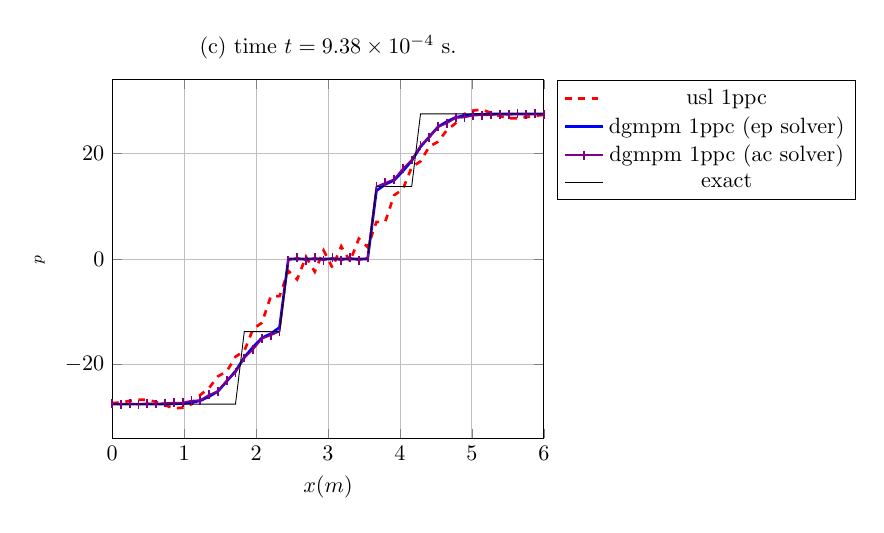
\begin{tikzpicture}[scale=0.8]
\begin{axis}[xlabel=$x (m)$,ylabel=$\eps^p$,ymajorgrids=true,xmajorgrids=true,legend pos=outer north east,title={(c) time $t = 9.38\times 10^{-4} $ s.},xmin=0.,xmax=6.]
\addplot[Red,very thick,mark=none,dashed] coordinates {(0.0,-27.331872449853556) (0.12244897959183673,-27.174400085417467) (0.24489795918367346,-26.904779830121768) (0.36734693877551017,-26.69301343005911) (0.4897959183673469,-26.683543140751915) (0.6122448979591837,-27.106963962300345) (0.7346938775510203,-27.704030887608354) (0.8571428571428571,-28.33906014232905) (0.9795918367346939,-28.167172814076366) (1.1020408163265305,-27.53334986092529) (1.2244897959183674,-25.775044707062726) (1.346938775510204,-24.466615882102165) (1.4693877551020407,-22.247186500301964) (1.5918367346938775,-21.33079179039491) (1.7142857142857142,-18.523714044368063) (1.836734693877551,-17.44233776410034) (1.9591836734693877,-13.237799741628182) (2.0816326530612246,-12.0894356407598) (2.204081632653061,-7.096371776087362) (2.326530612244898,-7.032925295785245) (2.4489795918367347,-2.2620897664972315) (2.571428571428571,-3.858668388515009) (2.693877551020408,0.4300541105363164) (2.816326530612245,-2.410115988529146) (2.9387755102040813,1.6326922086221445) (3.061224489795918,-1.6326922086221325) (3.183673469387755,2.410115988529122) (3.306122448979592,-0.43005411053631265) (3.4285714285714284,3.858668388514974) (3.5510204081632653,2.2620897664972395) (3.673469387755102,7.032925295785231) (3.7959183673469385,7.096371776087392) (3.9183673469387754,12.089435640759786) (4.040816326530612,13.237799741628214) (4.163265306122449,17.442337764100337) (4.285714285714286,18.523714044368088) (4.408163265306122,21.330791790394894) (4.530612244897959,22.247186500301982) (4.653061224489796,24.466615882102147) (4.775510204081632,25.775044707062744) (4.8979591836734695,27.53334986092529) (5.020408163265306,28.167172814076363) (5.142857142857142,28.33906014232903) (5.26530612244898,27.70403088760834) (5.387755102040816,27.106963962300348) (5.5102040816326525,26.683543140751933) (5.63265306122449,26.693013430059132) (5.755102040816326,26.904779830121797) (5.877551020408163,27.17440008541749) (6.0,27.331872449853574) };
\addplot[Blue,very thick,mark=none,solid] coordinates {(0.0,-27.517363397075158) (0.12244897959183673,-27.51732379155038) (0.24489795918367346,-27.517228936294842) (0.36734693877551017,-27.516689788484122) (0.4897959183673469,-27.51556852970287) (0.6122448979591837,-27.51025382248486) (0.7346938775510203,-27.500198710367762) (0.8571428571428571,-27.46081288016468) (0.9795918367346939,-27.394149463815687) (1.1020408163265305,-27.182111927326964) (1.2244897959183674,-26.86831399158136) (1.346938775510204,-26.07814929006618) (1.4693877551020407,-25.08839352872312) (1.5918367346938775,-23.189519000405884) (1.7142857142857142,-21.27348955232935) (1.836734693877551,-18.64183859399968) (1.9591836734693877,-16.67485639518814) (2.0816326530612246,-14.95207519835609) (2.204081632653061,-14.149762008703409) (2.326530612244898,-12.971197310204563) (2.4489795918367347,3.556080111931078e-14) (2.571428571428571,1.8614128550443383e-14) (2.693877551020408,1.1448988934369504e-14) (2.816326530612245,3.15403661725491e-14) (2.9387755102040813,2.1706952110207872e-14) (3.061224489795918,1.837643246978256e-14) (3.183673469387755,7.175699018437745e-15) (3.306122448979592,1.6868189305533344e-14) (3.4285714285714284,1.74998305367758e-14) (3.5510204081632653,1.3502410778036318e-14) (3.673469387755102,12.971197310204614) (3.7959183673469385,14.149762008703469) (3.9183673469387754,14.952075198356113) (4.040816326530612,16.67485639518816) (4.163265306122449,18.641838593999687) (4.285714285714286,21.273489552329384) (4.408163265306122,23.189519000405888) (4.530612244897959,25.088393528723138) (4.653061224489796,26.07814929006618) (4.775510204081632,26.868313991581342) (4.8979591836734695,27.182111927326957) (5.020408163265306,27.3941494638157) (5.142857142857142,27.46081288016466) (5.26530612244898,27.500198710367762) (5.387755102040816,27.51025382248485) (5.5102040816326525,27.515568529702865) (5.63265306122449,27.51668978848415) (5.755102040816326,27.517228936294806) (5.877551020408163,27.517323791550382) (6.0,27.517363397075165) };
\addplot[Purple,thick,mark=|,solid] coordinates {(0.0,-27.455491898583844) (0.12244897959183673,-27.52990791746212) (0.24489795918367346,-27.39669410111553) (0.36734693877551017,-27.56069772218648) (0.4897959183673469,-27.354208534961813) (0.6122448979591837,-27.484169218141297) (0.7346938775510203,-27.30529154707286) (0.8571428571428571,-27.260887430891447) (0.9795918367346939,-27.234362200737557) (1.1020408163265305,-26.87048565463221) (1.2244897959183674,-26.76603983934888) (1.346938775510204,-25.75807449243556) (1.4693877551020407,-25.06955937174821) (1.5918367346938775,-23.02673771458467) (1.7142857142857142,-21.509235536573875) (1.836734693877551,-18.773874989550777) (1.9591836734693877,-17.141311478227397) (2.0816326530612246,-15.098912535609557) (2.204081632653061,-14.451161421148855) (2.326530612244898,-13.715612700621918) (2.4489795918367347,-0.23693029878140853) (2.571428571428571,0.24220658661539068) (2.693877551020408,-0.22882318056987147) (2.816326530612245,0.2316928153217551) (2.9387755102040813,-0.22713962166300733) (3.061224489795918,0.22713962166305024) (3.183673469387755,-0.2316928153217785) (3.306122448979592,0.22882318056992768) (3.4285714285714284,-0.24220658661539307) (3.5510204081632653,0.23693029878141705) (3.673469387755102,13.71561270062201) (3.7959183673469385,14.451161421148875) (3.9183673469387754,15.098912535609603) (4.040816326530612,17.141311478227408) (4.163265306122449,18.77387498955077) (4.285714285714286,21.509235536573904) (4.408163265306122,23.026737714584694) (4.530612244897959,25.06955937174818) (4.653061224489796,25.758074492435522) (4.775510204081632,26.766039839348913) (4.8979591836734695,26.870485654632194) (5.020408163265306,27.23436220073757) (5.142857142857142,27.260887430891422) (5.26530612244898,27.305291547072898) (5.387755102040816,27.484169218141297) (5.5102040816326525,27.354208534961796) (5.63265306122449,27.560697722186475) (5.755102040816326,27.39669410111557) (5.877551020408163,27.529907917462097) (6.0,27.455491898583855) };
\addplot[black,thin,mark=none,solid] coordinates {(0.0,-27.517375820951077) (0.12244897959183673,-27.517375820951077) (0.24489795918367346,-27.517375820951077) (0.36734693877551017,-27.517375820951077) (0.4897959183673469,-27.517375820951077) (0.6122448979591837,-27.517375820951077) (0.7346938775510203,-27.517375820951077) (0.8571428571428571,-27.517375820951077) (0.9795918367346939,-27.517375820951077) (1.1020408163265305,-27.517375820951077) (1.2244897959183674,-27.517375820951077) (1.346938775510204,-27.517375820951077) (1.4693877551020407,-27.517375820951077) (1.5918367346938775,-27.517375820951077) (1.7142857142857142,-27.517375820951077) (1.836734693877551,-13.758687910475539) (1.9591836734693877,-13.758687910475539) (2.0816326530612246,-13.758687910475539) (2.204081632653061,-13.758687910475539) (2.326530612244898,-13.758687910475539) (2.4489795918367347,-0.0) (2.571428571428571,-0.0) (2.693877551020408,-0.0) (2.816326530612245,-0.0) (2.9387755102040813,-0.0) (3.061224489795918,-0.0) (3.183673469387755,-0.0) (3.306122448979592,-0.0) (3.4285714285714284,-0.0) (3.5510204081632653,-0.0) (3.673469387755102,13.758687910475539) (3.7959183673469385,13.758687910475539) (3.9183673469387754,13.758687910475539) (4.040816326530612,13.758687910475539) (4.163265306122449,13.758687910475539) (4.285714285714286,27.517375820951077) (4.408163265306122,27.517375820951077) (4.530612244897959,27.517375820951077) (4.653061224489796,27.517375820951077) (4.775510204081632,27.517375820951077) (4.8979591836734695,27.517375820951077) (5.020408163265306,27.517375820951077) (5.142857142857142,27.517375820951077) (5.26530612244898,27.517375820951077) (5.387755102040816,27.517375820951077) (5.5102040816326525,27.517375820951077) (5.63265306122449,27.517375820951077) (5.755102040816326,27.517375820951077) (5.877551020408163,27.517375820951077) (6.0,27.517375820951077) };
\legend{usl 1ppc,dgmpm 1ppc (ep solver),dgmpm 1ppc (ac solver),exact}
\end{axis}
\end{tikzpicture}
%%% Local Variables:
%%% mode: latex
%%% TeX-master: "../../mainManuscript"
%%% End:
}
  \caption{elastic-plastic RP velo}
  \label{fig:velo_elastoplastic_RP}
\end{figure}
Comparison with mpm for 1ppc and 2ppcs with RK2
\begin{figure}[h!]
  \centering
  {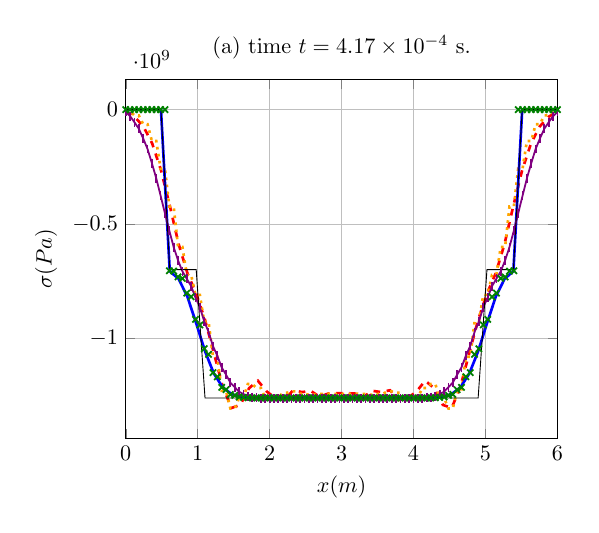
\begin{tikzpicture}[scale=0.8]
\begin{axis}[xlabel=$x (m)$,ylabel=$\sigma (Pa)$,ymajorgrids=true,xmajorgrids=true,legend pos=outer north east,title={(a) time $t = 4.17\times 10^{-4} $ s.},xmin=0.,xmax=6.]
\addplot[Red,very thick,mark=none,dashed] coordinates {(0.0,-8433215.03790355) (0.12244897959183673,-31379937.150059074) (0.24489795918367346,-73325965.87671247) (0.36734693877551017,-147815909.35881704) (0.4897959183673469,-264501011.32373637) (0.6122448979591837,-419797360.6339785) (0.7346938775510203,-586994803.1537646) (0.8571428571428571,-715242874.2277462) (0.9795918367346939,-804731796.1198385) (1.1020408163265305,-919403784.9173691) (1.2244897959183674,-1063504114.033879) (1.346938775510204,-1209904754.949398) (1.4693877551020407,-1304654513.0867395) (1.5918367346938775,-1291382612.5749428) (1.7142857142857142,-1218226204.6353252) (1.836734693877551,-1185455835.0777807) (1.9591836734693877,-1232745182.470082) (2.0816326530612246,-1261396271.0817113) (2.204081632653061,-1270103667.4391637) (2.326530612244898,-1227250869.598082) (2.4489795918367347,-1235273389.504192) (2.571428571428571,-1229787858.686364) (2.693877551020408,-1255621316.42765) (2.816326530612245,-1241442333.7811728) (2.9387755102040813,-1239848703.7218106) (3.061224489795918,-1239848703.7218091) (3.183673469387755,-1241442333.781176) (3.306122448979592,-1255621316.4276485) (3.4285714285714284,-1229787858.6863654) (3.5510204081632653,-1235273389.5041904) (3.673469387755102,-1227250869.598084) (3.7959183673469385,-1270103667.439164) (3.9183673469387754,-1261396271.081712) (4.040816326530612,-1232745182.4700806) (4.163265306122449,-1185455835.0777805) (4.285714285714286,-1218226204.6353254) (4.408163265306122,-1291382612.5749435) (4.530612244897959,-1304654513.0867395) (4.653061224489796,-1209904754.9493968) (4.775510204081632,-1063504114.033878) (4.8979591836734695,-919403784.917369) (5.020408163265306,-804731796.1198374) (5.142857142857142,-715242874.2277458) (5.26530612244898,-586994803.1537648) (5.387755102040816,-419797360.63397753) (5.5102040816326525,-264501011.3237358) (5.63265306122449,-147815909.35881624) (5.755102040816326,-73325965.8767119) (5.877551020408163,-31379937.150058918) (6.0,-8433215.037903389) };
\addplot[Orange,very thick,mark=none,dotted] coordinates {(0.0,-6487195.537951967) (0.06060606060606061,-6487195.537951967) (0.12121212121212122,-25447135.693615116) (0.18181818181818182,-25447135.693615116) (0.24242424242424243,-63824482.75083538) (0.30303030303030304,-63824482.75083538) (0.36363636363636365,-137285465.71899292) (0.42424242424242425,-137285465.71899292) (0.48484848484848486,-258389785.15975574) (0.5454545454545454,-258389785.15975574) (0.6060606060606061,-423881256.5395016) (0.6666666666666667,-423881256.5395016) (0.7272727272727273,-600583024.9453735) (0.7878787878787878,-600583024.9453735) (0.8484848484848485,-722865198.6395395) (0.9090909090909092,-722865198.6395395) (0.9696969696969697,-810023297.3770617) (1.0303030303030303,-810023297.3770617) (1.0909090909090908,-927952236.069318) (1.1515151515151516,-927952236.069318) (1.2121212121212122,-1080376380.893252) (1.2727272727272727,-1080376380.893252) (1.3333333333333335,-1229973271.6895852) (1.393939393939394,-1229973271.6895852) (1.4545454545454546,-1306874646.9216745) (1.5151515151515151,-1306874646.9216745) (1.5757575757575757,-1260590226.5138178) (1.6363636363636365,-1260590226.5138178) (1.696969696969697,-1200189199.3767865) (1.7575757575757576,-1200189199.3767865) (1.8181818181818183,-1217233767.7027068) (1.878787878787879,-1217233767.7027068) (1.9393939393939394,-1260358671.3727095) (2.0,-1260358671.3727095) (2.0606060606060606,-1261618284.922131) (2.121212121212121,-1261618284.922131) (2.1818181818181817,-1238228645.818687) (2.2424242424242427,-1238228645.818687) (2.303030303030303,-1232247837.5911345) (2.3636363636363638,-1232247837.5911345) (2.4242424242424243,-1242565564.7913089) (2.484848484848485,-1242565564.7913089) (2.5454545454545454,-1247187746.3284252) (2.606060606060606,-1247187746.3284252) (2.666666666666667,-1243527207.3601675) (2.7272727272727275,-1243527207.3601675) (2.787878787878788,-1241890915.1682148) (2.8484848484848486,-1241890915.1682148) (2.909090909090909,-1243871775.6139772) (2.9696969696969697,-1243871775.6139772) (3.0303030303030303,-1243871775.613977) (3.090909090909091,-1243871775.613977) (3.1515151515151514,-1241890915.1682146) (3.2121212121212124,-1241890915.1682146) (3.272727272727273,-1243527207.3601675) (3.3333333333333335,-1243527207.3601675) (3.393939393939394,-1247187746.3284254) (3.4545454545454546,-1247187746.3284254) (3.515151515151515,-1242565564.7913094) (3.5757575757575757,-1242565564.7913094) (3.6363636363636367,-1232247837.591135) (3.6969696969696972,-1232247837.591135) (3.757575757575758,-1238228645.818687) (3.8181818181818183,-1238228645.818687) (3.878787878787879,-1261618284.9221313) (3.9393939393939394,-1261618284.9221313) (4.0,-1260358671.37271) (4.0606060606060606,-1260358671.37271) (4.121212121212121,-1217233767.7027078) (4.181818181818182,-1217233767.7027078) (4.242424242424242,-1200189199.3767872) (4.303030303030303,-1200189199.3767872) (4.363636363636363,-1260590226.5138175) (4.424242424242425,-1260590226.5138175) (4.484848484848485,-1306874646.9216745) (4.545454545454546,-1306874646.9216745) (4.606060606060606,-1229973271.6895852) (4.666666666666667,-1229973271.6895852) (4.7272727272727275,-1080376380.893252) (4.787878787878788,-1080376380.893252) (4.848484848484849,-927952236.069318) (4.909090909090909,-927952236.069318) (4.96969696969697,-810023297.3770617) (5.03030303030303,-810023297.3770617) (5.090909090909091,-722865198.6395395) (5.151515151515151,-722865198.6395395) (5.212121212121212,-600583024.9453732) (5.2727272727272725,-600583024.9453732) (5.333333333333334,-423881256.5395015) (5.3939393939393945,-423881256.5395015) (5.454545454545455,-258389785.1597556) (5.515151515151516,-258389785.1597556) (5.575757575757576,-137285465.71899268) (5.636363636363637,-137285465.71899268) (5.696969696969697,-63824482.75083506) (5.757575757575758,-63824482.75083506) (5.818181818181818,-25447135.69361456) (5.878787878787879,-25447135.69361456) (5.9393939393939394,-6487195.537951966) (6.0,-6487195.537951966) };
\addplot[Blue,very thick,mark=none,solid] coordinates {(0.0,-3.2561158711216654e-07) (0.12244897959183673,-6.54162606232603e-22) (0.24489795918367346,0.0) (0.36734693877551017,3.2561158711216643e-07) (0.4897959183673469,-4.884173806682499e-07) (0.6122448979591837,-706703995.0062007) (0.7346938775510203,-739923853.3127105) (0.8571428571428571,-818114621.3278772) (0.9795918367346939,-934350667.0858994) (1.1020408163265305,-1056745717.4113452) (1.2244897959183674,-1153785079.176232) (1.346938775510204,-1213891661.9862223) (1.4693877551020407,-1243675875.166416) (1.5918367346938775,-1255667377.4619899) (1.7142857142857142,-1259628756.7765899) (1.836734693877551,-1260708382.472525) (1.9591836734693877,-1260951555.06527) (2.0816326530612246,-1260996741.6987677) (2.204081632653061,-1261003631.246593) (2.326530612244898,-1261004484.7294881) (2.4489795918367347,-1261004569.3136225) (2.571428571428571,-1261004575.8625927) (2.693877551020408,-1261004576.2443771) (2.816326530612245,-1261004576.2601426) (2.9387755102040813,-1261004576.2605536) (3.061224489795918,-1261004576.2605536) (3.183673469387755,-1261004576.2601426) (3.306122448979592,-1261004576.2443776) (3.4285714285714284,-1261004575.862593) (3.5510204081632653,-1261004569.3136227) (3.673469387755102,-1261004484.7294881) (3.7959183673469385,-1261003631.2465928) (3.9183673469387754,-1260996741.6987677) (4.040816326530612,-1260951555.0652697) (4.163265306122449,-1260708382.4725246) (4.285714285714286,-1259628756.7765894) (4.408163265306122,-1255667377.4619899) (4.530612244897959,-1243675875.1664157) (4.653061224489796,-1213891661.9862223) (4.775510204081632,-1153785079.176232) (4.8979591836734695,-1056745717.4113454) (5.020408163265306,-934350667.0858992) (5.142857142857142,-818114621.327877) (5.26530612244898,-739923853.3127109) (5.387755102040816,-706703995.0062011) (5.5102040816326525,-4.884173806682498e-07) (5.63265306122449,0.0) (5.755102040816326,-4.884173806682498e-07) (5.877551020408163,0.0) (6.0,-4.884173806682498e-07) };
\addplot[Purple,thick,mark=|,solid] coordinates {(0.0,-10397459.452423438) (0.06060606060606061,-28629486.986752886) (0.12121212121212122,-55131928.25663453) (0.18181818181818182,-83646270.11748616) (0.24242424242424243,-125654961.11636907) (0.30303030303030304,-172284594.0778725) (0.36363636363636365,-234043640.37607408) (0.42424242424242425,-300242328.04419184) (0.48484848484848486,-376432798.7765728) (0.5454545454545454,-453818751.237467) (0.6060606060606061,-529414416.2674847) (0.6666666666666667,-601300645.223565) (0.7272727272727273,-659382521.0565735) (0.7878787878787878,-707161316.1944203) (0.8484848484848485,-739803034.1794951) (0.9090909090909092,-772004069.950914) (0.9696969696969697,-822251842.2420584) (1.0303030303030303,-864154645.8439147) (1.0909090909090908,-925876995.0130453) (1.1515151515151516,-972279835.0233293) (1.2121212121212122,-1033743758.8085552) (1.2727272727272727,-1076108794.246372) (1.3333333333333335,-1126940545.3466995) (1.393939393939394,-1158983016.4555871) (1.4545454545454546,-1193843324.3931508) (1.5151515151515151,-1213855388.0055108) (1.5757575757575757,-1233610942.154643) (1.6363636363636365,-1243855259.0681229) (1.696969696969697,-1252984033.6395779) (1.7575757575757576,-1257191611.231863) (1.8181818181818183,-1260529554.0622826) (1.878787878787879,-1261847454.6142046) (1.9393939393939394,-1262731019.2058864) (2.0,-1262988692.0798318) (2.0606060606060606,-1263095211.659083) (2.121212121212121,-1263057284.7251215) (2.1818181818181817,-1263041880.329979) (2.2424242424242427,-1262967457.2713077) (2.303030303030303,-1262995543.9612422) (2.3636363636363638,-1262899504.1699014) (2.4242424242424243,-1262951100.2551603) (2.484848484848485,-1262880485.8465211) (2.5454545454545454,-1262941766.4492297) (2.606060606060606,-1262877340.9880557) (2.666666666666667,-1262975476.3750632) (2.7272727272727275,-1262864851.3501468) (2.787878787878788,-1263076922.0461023) (2.8484848484848486,-1262804308.8537025) (2.909090909090909,-1263257734.3780806) (2.9696969696969697,-1262658504.412126) (3.0303030303030303,-1262658504.4121263) (3.090909090909091,-1263257734.3780804) (3.1515151515151514,-1262804308.8537023) (3.2121212121212124,-1263076922.046102) (3.272727272727273,-1262864851.3501468) (3.3333333333333335,-1262975476.375064) (3.393939393939394,-1262877340.988056) (3.4545454545454546,-1262941766.4492295) (3.515151515151515,-1262880485.8465207) (3.5757575757575757,-1262951100.2551603) (3.6363636363636367,-1262899504.169902) (3.6969696969696972,-1262995543.961243) (3.757575757575758,-1262967457.2713082) (3.8181818181818183,-1263041880.329979) (3.878787878787879,-1263057284.7251215) (3.9393939393939394,-1263095211.6590827) (4.0,-1262988692.0798314) (4.0606060606060606,-1262731019.205886) (4.121212121212121,-1261847454.6142046) (4.181818181818182,-1260529554.0622826) (4.242424242424242,-1257191611.2318633) (4.303030303030303,-1252984033.6395783) (4.363636363636363,-1243855259.0681233) (4.424242424242425,-1233610942.1546435) (4.484848484848485,-1213855388.0055118) (4.545454545454546,-1193843324.3931518) (4.606060606060606,-1158983016.4555879) (4.666666666666667,-1126940545.3467004) (4.7272727272727275,-1076108794.2463727) (4.787878787878788,-1033743758.8085555) (4.848484848484849,-972279835.0233293) (4.909090909090909,-925876995.0130455) (4.96969696969697,-864154645.8439149) (5.03030303030303,-822251842.2420586) (5.090909090909091,-772004069.9509139) (5.151515151515151,-739803034.1794952) (5.212121212121212,-707161316.1944203) (5.2727272727272725,-659382521.0565742) (5.333333333333334,-601300645.2235655) (5.3939393939393945,-529414416.26748544) (5.454545454545455,-453818751.23746747) (5.515151515151516,-376432798.776573) (5.575757575757576,-300242328.0441918) (5.636363636363637,-234043640.37607414) (5.696969696969697,-172284594.0778724) (5.757575757575758,-125654961.1163687) (5.818181818181818,-83646270.11748542) (5.878787878787879,-55131928.256634116) (5.9393939393939394,-28629486.98675295) (6.0,-10397459.452423694) };
\addplot[Green,thick,mark=x,only marks] coordinates {(0.0,-9.938985241112485e-07) (0.06060606060606061,-1.2853825856739185e-06) (0.12121212121212122,8.201488924992559e-07) (0.18181818181818182,4.822974559494094e-07) (0.24242424242424243,-9.83648482392308e-07) (0.30303030303030304,-1.2956326273928566e-06) (0.36363636363636365,1.9586488831001813e-06) (0.42424242424242425,2.5999133364701503e-06) (0.48484848484848486,-1.4790882727589648e-06) (0.5454545454545454,-1.4514160112505328e-06) (0.6060606060606061,-704729842.2455659) (0.6666666666666667,-706002047.1314592) (0.7272727272727273,-731613409.0827894) (0.7878787878787878,-738307360.3254093) (0.8484848484848485,-802443845.4106181) (0.9090909090909092,-818702029.0002648) (0.9696969696969697,-917273418.4084023) (1.0303030303030303,-941457325.3246986) (1.0909090909090908,-1045498983.9435152) (1.1515151515151516,-1070147015.0174686) (1.2121212121212122,-1150104083.776542) (1.2727272727272727,-1168347225.6924338) (1.3333333333333335,-1214623647.0248165) (1.393939393939394,-1224762462.1158886) (1.4545454545454546,-1245337865.7733397) (1.5151515151515151,-1249651955.7951238) (1.5757575757575757,-1256756187.728854) (1.6363636363636365,-1258176137.8011208) (1.696969696969697,-1260087550.9276555) (1.7575757575757576,-1260449997.1780932) (1.8181818181818183,-1260849081.875068) (1.878787878787879,-1260920429.9830258) (1.9393939393939394,-1260984677.091578) (2.0,-1260995458.2161036) (2.0606060606060606,-1261002466.8790119) (2.121212121212121,-1261003454.0601096) (2.1818181818181817,-1261004228.03729) (2.2424242424242427,-1261004332.3287823) (2.303030303030303,-1261004658.4164412) (2.3636363636363638,-1261004353.5092869) (2.4242424242424243,-1261005248.8606844) (2.484848484848485,-1261004976.0401845) (2.5454545454545454,-1261004543.3087149) (2.606060606060606,-1261003848.6940825) (2.666666666666667,-1261005173.6392112) (2.7272727272727275,-1261003422.415637) (2.787878787878788,-1261005964.7480397) (2.8484848484848486,-1261003205.9507174) (2.909090909090909,-1261018212.4618385) (2.9696969696969697,-1260990356.2943678) (3.0303030303030303,-1260990356.2943668) (3.090909090909091,-1261018212.4618378) (3.1515151515151514,-1261003205.950717) (3.2121212121212124,-1261005964.7480397) (3.272727272727273,-1261003422.415637) (3.3333333333333335,-1261005173.6392105) (3.393939393939394,-1261003848.6940827) (3.4545454545454546,-1261004543.3087158) (3.515151515151515,-1261004976.0401855) (3.5757575757575757,-1261005248.860685) (3.6363636363636367,-1261004353.5092869) (3.6969696969696972,-1261004658.4164414) (3.757575757575758,-1261004332.328783) (3.8181818181818183,-1261004228.0372908) (3.878787878787879,-1261003454.0601094) (3.9393939393939394,-1261002466.8790114) (4.0,-1260995458.2161038) (4.0606060606060606,-1260984677.091578) (4.121212121212121,-1260920429.9830256) (4.181818181818182,-1260849081.8750677) (4.242424242424242,-1260449997.1780937) (4.303030303030303,-1260087550.9276562) (4.363636363636363,-1258176137.8011205) (4.424242424242425,-1256756187.728854) (4.484848484848485,-1249651955.795124) (4.545454545454546,-1245337865.7733407) (4.606060606060606,-1224762462.1158893) (4.666666666666667,-1214623647.024817) (4.7272727272727275,-1168347225.692434) (4.787878787878788,-1150104083.7765424) (4.848484848484849,-1070147015.0174688) (4.909090909090909,-1045498983.9435161) (4.96969696969697,-941457325.3246986) (5.03030303030303,-917273418.4084023) (5.090909090909091,-818702029.0002651) (5.151515151515151,-802443845.4106187) (5.212121212121212,-738307360.3254088) (5.2727272727272725,-731613409.0827891) (5.333333333333334,-706002047.1314601) (5.3939393939393945,-704729842.2455676) (5.454545454545455,-9.052507597537938e-07) (5.515151515151516,-7.228071758070392e-07) (5.575757575757576,8.567216523351019e-07) (5.636363636363637,7.713362832257307e-07) (5.696969696969697,-5.847958087280893e-07) (5.757575757575758,-7.176505397205777e-07) (5.818181818181818,1.1498742353244018e-06) (5.878787878787879,1.4550184615729307e-06) (5.9393939393939394,-2.547964815114839e-06) (6.0,-2.336208991567657e-06) };
\addplot[black,thin,mark=none,solid] coordinates {(0.0,-0.0) (0.12244897959183673,-0.0) (0.24489795918367346,-0.0) (0.36734693877551017,-0.0) (0.4897959183673469,-0.0) (0.6122448979591837,-700000000.0) (0.7346938775510203,-700000000.0) (0.8571428571428571,-700000000.0) (0.9795918367346939,-700000000.0) (1.1020408163265305,-1261004576.260559) (1.2244897959183674,-1261004576.260559) (1.346938775510204,-1261004576.260559) (1.4693877551020407,-1261004576.260559) (1.5918367346938775,-1261004576.260559) (1.7142857142857142,-1261004576.260559) (1.836734693877551,-1261004576.260559) (1.9591836734693877,-1261004576.260559) (2.0816326530612246,-1261004576.260559) (2.204081632653061,-1261004576.260559) (2.326530612244898,-1261004576.260559) (2.4489795918367347,-1261004576.260559) (2.571428571428571,-1261004576.260559) (2.693877551020408,-1261004576.260559) (2.816326530612245,-1261004576.260559) (2.9387755102040813,-1261004576.260559) (3.061224489795918,-1261004576.260559) (3.183673469387755,-1261004576.260559) (3.306122448979592,-1261004576.260559) (3.4285714285714284,-1261004576.260559) (3.5510204081632653,-1261004576.260559) (3.673469387755102,-1261004576.260559) (3.7959183673469385,-1261004576.260559) (3.9183673469387754,-1261004576.260559) (4.040816326530612,-1261004576.260559) (4.163265306122449,-1261004576.260559) (4.285714285714286,-1261004576.260559) (4.408163265306122,-1261004576.260559) (4.530612244897959,-1261004576.260559) (4.653061224489796,-1261004576.260559) (4.775510204081632,-1261004576.260559) (4.8979591836734695,-1261004576.260559) (5.020408163265306,-700000000.0) (5.142857142857142,-700000000.0) (5.26530612244898,-700000000.0) (5.387755102040816,-700000000.0) (5.5102040816326525,-0.0) (5.63265306122449,-0.0) (5.755102040816326,-0.0) (5.877551020408163,-0.0) (6.0,-0.0) };
%\legend{usl 1ppc,usl 2ppc,dgmpm 1ppc,dgmpm 2ppc,dgmpm 2ppc (RK2),exact}
\end{axis}
\end{tikzpicture}
%%% Local Variables:
%%% mode: latex
%%% TeX-master: "../../mainManuscript"
%%% End:
}
  {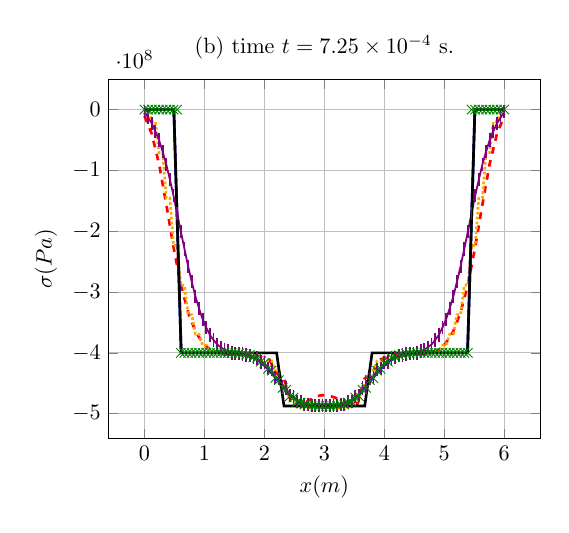
\begin{tikzpicture}[scale=0.8]
\begin{axis}[xlabel=$x (m)$,ylabel=$\sigma (Pa)$,ymajorgrids=true,xmajorgrids=true,legend pos=outer north east,title={(b) time $t = 7.25\times 10^{-4} $ s.}]
\addplot[Red,very thick,mark=none,dashed,mark size=3pt] coordinates {(0.0,-10477027.22040739) (0.12244897959183673,-40202439.77672757) (0.24489795918367346,-90268409.98400429) (0.36734693877551017,-157917330.96394995) (0.4897959183673469,-229098117.24026006) (0.6122448979591837,-290170966.79273176) (0.7346938775510203,-335449952.79523534) (0.8571428571428571,-366063963.8356788) (0.9795918367346939,-384934670.81956863) (1.1020408163265305,-394978768.22705775) (1.2244897959183674,-399539747.49342227) (1.346938775510204,-401064801.98949975) (1.4693877551020407,-401261686.3649931) (1.5918367346938775,-401362011.1717392) (1.7142857142857142,-402125702.7814173) (1.836734693877551,-402648608.50963366) (1.9591836734693877,-407517028.59914577) (2.0816326530612246,-411133976.99807984) (2.204081632653061,-433339939.374477) (2.326530612244898,-442099776.2163934) (2.4489795918367347,-483576545.68129754) (2.571428571428571,-481854124.4484605) (2.693877551020408,-481095256.73223835) (2.816326530612245,-473792554.1947772) (2.9387755102040813,-469732138.6842222) (3.061224489795918,-469732138.6842212) (3.183673469387755,-473792554.1947779) (3.306122448979592,-481095256.73223734) (3.4285714285714284,-481854124.4484616) (3.5510204081632653,-483576545.6812961) (3.673469387755102,-442099776.2163934) (3.7959183673469385,-433339939.3744765) (3.9183673469387754,-411133976.99807984) (4.040816326530612,-407517028.5991456) (4.163265306122449,-402648608.50963354) (4.285714285714286,-402125702.78141725) (4.408163265306122,-401362011.1717393) (4.530612244897959,-401261686.3649931) (4.653061224489796,-401064801.9894998) (4.775510204081632,-399539747.4934223) (4.8979591836734695,-394978768.22705775) (5.020408163265306,-384934670.81956846) (5.142857142857142,-366063963.83567846) (5.26530612244898,-335449952.79523504) (5.387755102040816,-290170966.7927308) (5.5102040816326525,-229098117.24025902) (5.63265306122449,-157917330.96394882) (5.755102040816326,-90268409.98400334) (5.877551020408163,-40202439.77672676) (6.0,-10477027.22040709) };
\addplot[Orange,very thick,mark=none,densely dotted,mark size=3pt] coordinates {(0.0,-1522322.3567553319) (0.06060606060606061,-1522322.3567553319) (0.12121212121212122,-19741546.758713853) (0.18181818181818182,-19741546.758713853) (0.24242424242424243,-70452847.74734518) (0.30303030303030304,-70452847.74734518) (0.36363636363636365,-145569726.72165304) (0.42424242424242425,-145569726.72165304) (0.48484848484848486,-223558621.35896367) (0.5454545454545454,-223558621.35896367) (0.6060606060606061,-288852526.8705149) (0.6666666666666667,-288852526.8705149) (0.7272727272727273,-337120167.47142065) (0.7878787878787878,-337120167.47142065) (0.8484848484848485,-369182466.2528492) (0.9090909090909092,-369182466.2528492) (0.9696969696969697,-387695734.7050902) (1.0303030303030303,-387695734.7050902) (1.0909090909090908,-396787746.7545124) (1.1515151515151516,-396787746.7545124) (1.2121212121212122,-400346482.5664338) (1.2727272727272727,-400346482.5664338) (1.3333333333333335,-401071106.301628) (1.393939393939394,-401071106.301628) (1.4545454545454546,-401189158.25601304) (1.5151515151515151,-401189158.25601304) (1.5757575757575757,-401411626.48080814) (1.6363636363636365,-401411626.48080814) (1.696969696969697,-401847412.82243955) (1.7575757575757576,-401847412.82243955) (1.8181818181818183,-402892812.90166867) (1.878787878787879,-402892812.90166867) (1.9393939393939394,-405871331.09740126) (2.0,-405871331.09740126) (2.0606060606060606,-413271912.46434987) (2.121212121212121,-413271912.46434987) (2.1818181818181817,-428650643.90280265) (2.2424242424242427,-428650643.90280265) (2.303030303030303,-453302573.20518476) (2.3636363636363638,-453302573.20518476) (2.4242424242424243,-478258276.212825) (2.484848484848485,-478258276.212825) (2.5454545454545454,-489476664.1834195) (2.606060606060606,-489476664.1834195) (2.666666666666667,-489046885.64068294) (2.7272727272727275,-489046885.64068294) (2.787878787878788,-491447894.73413926) (2.8484848484848486,-491447894.73413926) (2.909090909090909,-486436945.7103945) (2.9696969696969697,-486436945.7103945) (3.0303030303030303,-486436945.7103945) (3.090909090909091,-486436945.7103945) (3.1515151515151514,-491447894.73413926) (3.2121212121212124,-491447894.73413926) (3.272727272727273,-489046885.64068294) (3.3333333333333335,-489046885.64068294) (3.393939393939394,-489476664.1834195) (3.4545454545454546,-489476664.1834195) (3.515151515151515,-478258276.212825) (3.5757575757575757,-478258276.212825) (3.6363636363636367,-453302573.2051846) (3.6969696969696972,-453302573.2051846) (3.757575757575758,-428650643.9028025) (3.8181818181818183,-428650643.9028025) (3.878787878787879,-413271912.46434987) (3.9393939393939394,-413271912.46434987) (4.0,-405871331.09740126) (4.0606060606060606,-405871331.09740126) (4.121212121212121,-402892812.90166855) (4.181818181818182,-402892812.90166855) (4.242424242424242,-401847412.82243955) (4.303030303030303,-401847412.82243955) (4.363636363636363,-401411626.4808081) (4.424242424242425,-401411626.4808081) (4.484848484848485,-401189158.25601304) (4.545454545454546,-401189158.25601304) (4.606060606060606,-401071106.3016279) (4.666666666666667,-401071106.3016279) (4.7272727272727275,-400346482.5664337) (4.787878787878788,-400346482.5664337) (4.848484848484849,-396787746.75451225) (4.909090909090909,-396787746.75451225) (4.96969696969697,-387695734.7050903) (5.03030303030303,-387695734.7050903) (5.090909090909091,-369182466.25284934) (5.151515151515151,-369182466.25284934) (5.212121212121212,-337120167.47142065) (5.2727272727272725,-337120167.47142065) (5.333333333333334,-288852526.8705149) (5.3939393939393945,-288852526.8705149) (5.454545454545455,-223558621.35896364) (5.515151515151516,-223558621.35896364) (5.575757575757576,-145569726.72165304) (5.636363636363637,-145569726.72165304) (5.696969696969697,-70452847.74734521) (5.757575757575758,-70452847.74734521) (5.818181818181818,-19741546.758713897) (5.878787878787879,-19741546.758713897) (5.9393939393939394,-1522322.3567553656) (6.0,-1522322.3567553656) };
\addplot[Blue,very thick,mark=none,solid,mark size=3pt] coordinates {(0.0,-0.016398596440346053) (0.12244897959183673,-0.06425322857955201) (0.24489795918367346,-0.7380674881804443) (0.36734693877551017,-2.12047390173559) (0.4897959183673469,-28.76271861558054) (0.6122448979591837,-400000015.4159754) (0.7346938775510203,-400000102.7573024) (0.8571428571428571,-400000598.1932516) (0.9795918367346939,-400003055.79803795) (1.1020408163265305,-400013747.0436081) (1.2244897959183674,-400054602.7199052) (1.346938775510204,-400191823.2382515) (1.4693877551020407,-400596672.6802674) (1.5918367346938775,-401644186.51493835) (1.7142857142857142,-404014374.4754996) (1.836734693877551,-408684632.25449073) (1.9591836734693877,-416652037.9726774) (2.0816326530612246,-428329061.0045163) (2.204081632653061,-442879954.5361007) (2.326530612244898,-458084443.80872595) (2.4489795918367347,-471157539.9020842) (2.571428571428571,-480164339.19475454) (2.693877551020408,-484944715.5259052) (2.816326530612245,-486779650.5319825) (2.9387755102040813,-487233015.60471344) (3.061224489795918,-487233015.60471344) (3.183673469387755,-486779650.5319825) (3.306122448979592,-484944715.5259052) (3.4285714285714284,-480164339.19475454) (3.5510204081632653,-471157539.9020842) (3.673469387755102,-458084443.80872613) (3.7959183673469385,-442879954.5361007) (3.9183673469387754,-428329061.0045163) (4.040816326530612,-416652037.9726776) (4.163265306122449,-408684632.2544908) (4.285714285714286,-404014374.4754996) (4.408163265306122,-401644186.5149382) (4.530612244897959,-400596672.68026733) (4.653061224489796,-400191823.2382513) (4.775510204081632,-400054602.7199051) (4.8979591836734695,-400013747.04360807) (5.020408163265306,-400003055.79803795) (5.142857142857142,-400000598.19325155) (5.26530612244898,-400000102.75730234) (5.387755102040816,-400000015.4159754) (5.5102040816326525,-28.762718512303003) (5.63265306122449,-2.1204742438100417) (5.755102040816326,-0.7380675867576459) (5.877551020408163,-0.06425320166977637) (6.0,-0.01639854380134023) };
\addplot[Purple,thick,mark=|,solid,mark size=3pt] coordinates {(0.0,-3643722.4057531543) (0.06060606060606061,-13253871.94771175) (0.12121212121212122,-22430884.29879855) (0.18181818181818182,-35710388.05852378) (0.24242424242424243,-49954062.55465116) (0.30303030303030304,-69199724.63429566) (0.36363636363636365,-90001064.05703217) (0.42424242424242425,-115227809.11229268) (0.48484848484848486,-141771114.02793142) (0.5454545454545454,-170682311.90803242) (0.6060606060606061,-200079540.00258502) (0.6666666666666667,-229014826.8013297) (0.7272727272727273,-257430278.9843493) (0.7878787878787878,-282843592.21811193) (0.8484848484848485,-306971268.4010445) (0.9090909090909092,-326667104.7497092) (0.9696969696969697,-344782488.29979676) (1.0303030303030303,-358341830.7310785) (1.0909090909090908,-370462827.7146289) (1.1515151515151516,-378821810.49726343) (1.2121212121212122,-386102976.6619535) (1.2727272727272727,-390706555.81264853) (1.3333333333333335,-394846891.2394369) (1.393939393939394,-396879468.6459066) (1.4545454545454546,-400395334.89461267) (1.5151515151515151,-400547253.1901776) (1.5757575757575757,-401393994.5226969) (1.6363636363636365,-401653877.80383056) (1.696969696969697,-403469259.9494932) (1.7575757575757576,-403991527.1056523) (1.8181818181818183,-407625905.94533336) (1.878787878787879,-408563059.4680144) (1.9393939393939394,-414922856.8689467) (2.0,-416374885.2462252) (2.0606060606060606,-425987877.61701065) (2.121212121212121,-427906862.049074) (2.1818181818181817,-440309840.98849624) (2.2424242424242427,-442439362.1915814) (2.303030303030303,-455885132.24318355) (2.3636363636363638,-457826856.56220615) (2.4242424242424243,-469809715.6908375) (2.484848484848485,-471219084.61224025) (2.5454545454545454,-479722411.6158245) (2.606060606060606,-480495963.9518887) (2.666666666666667,-485058185.3772167) (2.7272727272727275,-485348110.0144077) (2.787878787878788,-487020339.6946885) (2.8484848484848486,-487075458.5679951) (2.909090909090909,-487055267.13670456) (2.9696969696969697,-486361892.7822711) (3.0303030303030303,-486361892.78227144) (3.090909090909091,-487055267.1367042) (3.1515151515151514,-487075458.5679951) (3.2121212121212124,-487020339.69468886) (3.272727272727273,-485348110.0144077) (3.3333333333333335,-485058185.37721705) (3.393939393939394,-480495963.9518887) (3.4545454545454546,-479722411.6158245) (3.515151515151515,-471219084.61224025) (3.5757575757575757,-469809715.6908375) (3.6363636363636367,-457826856.5622063) (3.6969696969696972,-455885132.24318355) (3.757575757575758,-442439362.1915814) (3.8181818181818183,-440309840.98849636) (3.878787878787879,-427906862.0490741) (3.9393939393939394,-425987877.6170107) (4.0,-416374885.2462253) (4.0606060606060606,-414922856.86894685) (4.121212121212121,-408563059.46801454) (4.181818181818182,-407625905.94533336) (4.242424242424242,-403991527.1056523) (4.303030303030303,-403469259.9494934) (4.363636363636363,-401653877.80383074) (4.424242424242425,-401393994.522697) (4.484848484848485,-400547253.19017774) (4.545454545454546,-400395334.89461285) (4.606060606060606,-396879468.6459065) (4.666666666666667,-394846891.23943704) (4.7272727272727275,-390706555.81264836) (4.787878787878788,-386102976.66195333) (4.848484848484849,-378821810.4972633) (4.909090909090909,-370462827.71462864) (4.96969696969697,-358341830.73107857) (5.03030303030303,-344782488.29979694) (5.090909090909091,-326667104.7497094) (5.151515151515151,-306971268.4010446) (5.212121212121212,-282843592.21811193) (5.2727272727272725,-257430278.98434916) (5.333333333333334,-229014826.8013294) (5.3939393939393945,-200079540.00258464) (5.454545454545455,-170682311.90803197) (5.515151515151516,-141771114.0279309) (5.575757575757576,-115227809.11229216) (5.636363636363637,-90001064.0570316) (5.696969696969697,-69199724.63429512) (5.757575757575758,-49954062.55465064) (5.818181818181818,-35710388.058523305) (5.878787878787879,-22430884.29879819) (5.9393939393939394,-13253871.947711527) (6.0,-3643722.4057530854) };
\addplot[Green,thin,mark=x,only marks,mark size=3pt] coordinates {(0.0,-0.0009905544907868183) (0.06060606060606061,-0.001035109508555422) (0.12121212121212122,-0.005117191018500656) (0.18181818181818182,-0.0052978434023460315) (0.24242424242424243,-0.06517986204950546) (0.30303030303030304,-0.07566277987844348) (0.36363636363636365,-0.24962042121048697) (0.42424242424242425,-0.26937038060136104) (0.48484848484848486,-3.010621421655401) (0.5454545454545454,-5.186761151690843) (0.6060606060606061,-400000002.01453906) (0.6666666666666667,-400000003.4473042) (0.7272727272727273,-400000017.3967542) (0.7878787878787878,-400000028.78236) (0.8484848484848485,-400000129.15230495) (0.9090909090909092,-400000206.4599203) (0.9696969696969697,-400000827.7884989) (1.0303030303030303,-400001277.7907757) (1.0909090909090908,-400004594.5128382) (1.1515151515151516,-400006844.3811263) (1.2121212121212122,-400022128.58005637) (1.2727272727272727,-400031796.16010183) (1.3333333333333335,-400092597.4804089) (1.393939393939394,-400128278.6945615) (1.4545454545454546,-400336842.6530185) (1.5151515151515151,-400449754.98737735) (1.5757575757575757,-401065298.1117383) (1.6363636363636365,-401370713.3108358) (1.696969696969697,-402928435.1963118) (1.7575757575757576,-403631417.36330265) (1.8181818181818183,-406995518.8189568) (1.878787878787879,-408364026.9334509) (1.9393939393939394,-414524891.6433188) (2.0,-416759867.3744382) (2.0606060606060606,-426248412.6400655) (2.121212121212121,-429277915.8940706) (2.1818181818181817,-441434961.5049247) (2.2424242424242427,-444795234.23076177) (2.303030303030303,-457568597.61163) (2.3636363636363638,-460560432.82157856) (2.4242424242424243,-471355976.94533) (2.484848484848485,-473437539.61930424) (2.5454545454545454,-480581531.6160863) (2.606060606060606,-481669280.4693011) (2.666666666666667,-485226958.9355893) (2.7272727272727275,-485627667.237451) (2.787878787878788,-486879003.35388845) (2.8484848484848486,-486971605.60944414) (2.909090909090909,-487248222.53163636) (2.9696969696969697,-487258302.19873005) (3.0303030303030303,-487258302.19873005) (3.090909090909091,-487248222.53163636) (3.1515151515151514,-486971605.60944414) (3.2121212121212124,-486879003.35388845) (3.272727272727273,-485627667.237451) (3.3333333333333335,-485226958.9355893) (3.393939393939394,-481669280.4693011) (3.4545454545454546,-480581531.6160863) (3.515151515151515,-473437539.6193044) (3.5757575757575757,-471355976.94533) (3.6363636363636367,-460560432.82157856) (3.6969696969696972,-457568597.61163) (3.757575757575758,-444795234.23076177) (3.8181818181818183,-441434961.5049247) (3.878787878787879,-429277915.8940706) (3.9393939393939394,-426248412.64006543) (4.0,-416759867.3744382) (4.0606060606060606,-414524891.64331895) (4.121212121212121,-408364026.933451) (4.181818181818182,-406995518.8189568) (4.242424242424242,-403631417.3633025) (4.303030303030303,-402928435.1963118) (4.363636363636363,-401370713.3108358) (4.424242424242425,-401065298.11173844) (4.484848484848485,-400449754.9873774) (4.545454545454546,-400336842.65301853) (4.606060606060606,-400128278.6945615) (4.666666666666667,-400092597.48040897) (4.7272727272727275,-400031796.16010183) (4.787878787878788,-400022128.5800565) (4.848484848484849,-400006844.3811263) (4.909090909090909,-400004594.51283836) (4.96969696969697,-400001277.7907758) (5.03030303030303,-400000827.7884989) (5.090909090909091,-400000206.4599203) (5.151515151515151,-400000129.152305) (5.212121212121212,-400000028.7823601) (5.2727272727272725,-400000017.39675426) (5.333333333333334,-400000003.4473042) (5.3939393939393945,-400000002.014539) (5.454545454545455,-5.186761729700046) (5.515151515151516,-3.0106210293278775) (5.575757575757576,-0.26937051997179645) (5.636363636363637,-0.249620419252184) (5.696969696969697,-0.07566313892965675) (5.757575757575758,-0.06517962792185199) (5.818181818181818,-0.00529745130538514) (5.878787878787879,-0.005117314055782253) (5.9393939393939394,-0.0010346801603060291) (6.0,-0.0009902966227138578) };
\addplot[black,very thick,mark=pentagone*,solid,mark size=3pt] coordinates {(0.0,-0.0) (0.12244897959183673,-0.0) (0.24489795918367346,-0.0) (0.36734693877551017,-0.0) (0.4897959183673469,-0.0) (0.6122448979591837,-400000000.0) (0.7346938775510203,-400000000.0) (0.8571428571428571,-400000000.0) (0.9795918367346939,-400000000.0) (1.1020408163265305,-400000000.0) (1.2244897959183674,-400000000.0) (1.346938775510204,-400000000.0) (1.4693877551020407,-400000000.0) (1.5918367346938775,-400000000.0) (1.7142857142857142,-400000000.0) (1.836734693877551,-400000000.0) (1.9591836734693877,-400000000.0) (2.0816326530612246,-400000000.0) (2.204081632653061,-400000000.0) (2.326530612244898,-487287156.09439695) (2.4489795918367347,-487287156.09439695) (2.571428571428571,-487287156.09439695) (2.693877551020408,-487287156.09439695) (2.816326530612245,-487287156.09439695) (2.9387755102040813,-487287156.09439695) (3.061224489795918,-487287156.09439695) (3.183673469387755,-487287156.09439695) (3.306122448979592,-487287156.09439695) (3.4285714285714284,-487287156.09439695) (3.5510204081632653,-487287156.09439695) (3.673469387755102,-487287156.09439695) (3.7959183673469385,-400000000.0) (3.9183673469387754,-400000000.0) (4.040816326530612,-400000000.0) (4.163265306122449,-400000000.0) (4.285714285714286,-400000000.0) (4.408163265306122,-400000000.0) (4.530612244897959,-400000000.0) (4.653061224489796,-400000000.0) (4.775510204081632,-400000000.0) (4.8979591836734695,-400000000.0) (5.020408163265306,-400000000.0) (5.142857142857142,-400000000.0) (5.26530612244898,-400000000.0) (5.387755102040816,-400000000.0) (5.5102040816326525,-0.0) (5.63265306122449,-0.0) (5.755102040816326,-0.0) (5.877551020408163,-0.0) (6.0,-0.0) };
%\legend{usl 1ppc,usl 2ppc,dgmpm 1ppc,dgmpm 2ppc,dgmpm 2ppc (RK2),exact}
\end{axis}
\end{tikzpicture}
%%% Local Variables:
%%% mode: latex
%%% TeX-master: "../../mainManuscript"
%%% End:
}
  {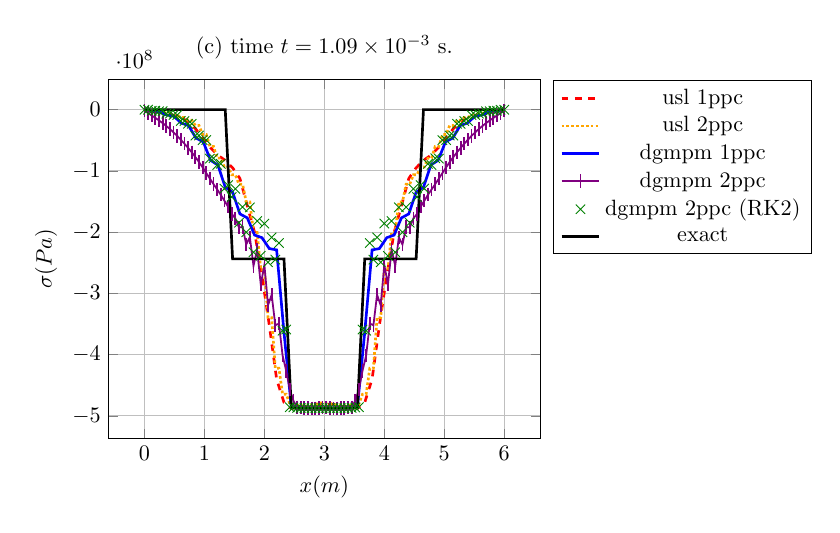
\begin{tikzpicture}[scale=0.8]
\begin{axis}[xlabel=$x (m)$,ylabel=$\sigma (Pa)$,ymajorgrids=true,xmajorgrids=true,legend pos=outer north east,title={(c) time $t = 1.09\times 10^{-3} $ s.}]
\addplot[Red,very thick,mark=none,dashed,mark size=3pt] coordinates {(0.0,-679166.0601331755) (0.12244897959183673,-2368189.594188208) (0.24489795918367346,-4606456.556212341) (0.36734693877551017,-6961578.395676694) (0.4897959183673469,-9332760.287028607) (0.6122448979591837,-12938682.464591796) (0.7346938775510203,-20102821.471402142) (0.8571428571428571,-32015823.341737133) (0.9795918367346939,-47676454.15860757) (1.1020408163265305,-62502940.42234602) (1.2244897959183674,-74544680.06037714) (1.346938775510204,-82775603.38522142) (1.4693877551020407,-94947363.4179823) (1.5918367346938775,-112415785.44002911) (1.7142857142857142,-156774491.63523546) (1.836734693877551,-200654618.50473383) (1.9591836734693877,-270646588.3413816) (2.0816326530612246,-351928629.9311485) (2.204081632653061,-440064160.15512294) (2.326530612244898,-477934424.91056436) (2.4489795918367347,-487815276.0764712) (2.571428571428571,-485351241.33413374) (2.693877551020408,-484406188.97201383) (2.816326530612245,-481035531.7602433) (2.9387755102040813,-481038509.8228564) (3.061224489795918,-481038509.8228558) (3.183673469387755,-481035531.7602443) (3.306122448979592,-484406188.9720135) (3.4285714285714284,-485351241.3341341) (3.5510204081632653,-487815276.07647014) (3.673469387755102,-477934424.9105651) (3.7959183673469385,-440064160.15512156) (3.9183673469387754,-351928629.931148) (4.040816326530612,-270646588.34138024) (4.163265306122449,-200654618.50473374) (4.285714285714286,-156774491.63523474) (4.408163265306122,-112415785.44002907) (4.530612244897959,-94947363.41798277) (4.653061224489796,-82775603.38522187) (4.775510204081632,-74544680.06037733) (4.8979591836734695,-62502940.42234604) (5.020408163265306,-47676454.158607304) (5.142857142857142,-32015823.341736842) (5.26530612244898,-20102821.471402) (5.387755102040816,-12938682.46459166) (5.5102040816326525,-9332760.287028512) (5.63265306122449,-6961578.395676572) (5.755102040816326,-4606456.55621225) (5.877551020408163,-2368189.594188123) (6.0,-679166.0601331636) };
\addplot[Orange,very thick,mark=none,densely dotted,mark size=3pt] coordinates {(0.0,-512829.37356199906) (0.06060606060606061,-512829.37356199906) (0.12121212121212122,-1685977.6907792736) (0.18181818181818182,-1685977.6907792736) (0.24242424242424243,-3409631.957049818) (0.30303030303030304,-3409631.957049818) (0.36363636363636365,-5994518.467970753) (0.42424242424242425,-5994518.467970753) (0.48484848484848486,-9186608.055434104) (0.5454545454545454,-9186608.055434104) (0.6060606060606061,-12632033.888351096) (0.6666666666666667,-12632033.888351096) (0.7272727272727273,-17308370.109125804) (0.7878787878787878,-17308370.109125804) (0.8484848484848485,-25927147.931033082) (0.9090909090909092,-25927147.931033082) (0.9696969696969697,-40719694.7337496) (1.0303030303030303,-40719694.7337496) (1.0909090909090908,-60222421.752752535) (1.1515151515151516,-60222421.752752535) (1.2121212121212122,-79232798.7243564) (1.2727272727272727,-79232798.7243564) (1.3333333333333335,-93917910.36545579) (1.393939393939394,-93917910.36545579) (1.4545454545454546,-106296964.05562654) (1.5151515151515151,-106296964.05562654) (1.5757575757575757,-121857025.50296684) (1.6363636363636365,-121857025.50296684) (1.696969696969697,-150591571.19633642) (1.7575757575757576,-150591571.19633642) (1.8181818181818183,-200655220.68880683) (1.878787878787879,-200655220.68880683) (1.9393939393939394,-261493503.50548327) (2.0,-261493503.50548327) (2.0606060606060606,-339524928.63039523) (2.121212121212121,-339524928.63039523) (2.1818181818181817,-422131801.353524) (2.2424242424242427,-422131801.353524) (2.303030303030303,-464494091.2915379) (2.3636363636363638,-464494091.2915379) (2.4242424242424243,-480288801.84594995) (2.484848484848485,-480288801.84594995) (2.5454545454545454,-482971319.0696361) (2.606060606060606,-482971319.0696361) (2.666666666666667,-484006263.5397973) (2.7272727272727275,-484006263.5397973) (2.787878787878788,-481823971.2401126) (2.8484848484848486,-481823971.2401126) (2.909090909090909,-478820708.8588188) (2.9696969696969697,-478820708.8588188) (3.0303030303030303,-478820708.8588188) (3.090909090909091,-478820708.8588188) (3.1515151515151514,-481823971.24011296) (3.2121212121212124,-481823971.24011296) (3.272727272727273,-484006263.53979766) (3.3333333333333335,-484006263.53979766) (3.393939393939394,-482971319.0696361) (3.4545454545454546,-482971319.0696361) (3.515151515151515,-480288801.84594995) (3.5757575757575757,-480288801.84594995) (3.6363636363636367,-464494091.2915379) (3.6969696969696972,-464494091.2915379) (3.757575757575758,-422131801.3535244) (3.8181818181818183,-422131801.3535244) (3.878787878787879,-339524928.6303949) (3.9393939393939394,-339524928.6303949) (4.0,-261493503.50548312) (4.0606060606060606,-261493503.50548312) (4.121212121212121,-200655220.68880683) (4.181818181818182,-200655220.68880683) (4.242424242424242,-150591571.1963363) (4.303030303030303,-150591571.1963363) (4.363636363636363,-121857025.50296697) (4.424242424242425,-121857025.50296697) (4.484848484848485,-106296964.05562642) (4.545454545454546,-106296964.05562642) (4.606060606060606,-93917910.36545563) (4.666666666666667,-93917910.36545563) (4.7272727272727275,-79232798.7243563) (4.787878787878788,-79232798.7243563) (4.848484848484849,-60222421.752752505) (4.909090909090909,-60222421.752752505) (4.96969696969697,-40719694.73374956) (5.03030303030303,-40719694.73374956) (5.090909090909091,-25927147.93103303) (5.151515151515151,-25927147.93103303) (5.212121212121212,-17308370.109125733) (5.2727272727272725,-17308370.109125733) (5.333333333333334,-12632033.888351053) (5.3939393939393945,-12632033.888351053) (5.454545454545455,-9186608.05543412) (5.515151515151516,-9186608.05543412) (5.575757575757576,-5994518.467970843) (5.636363636363637,-5994518.467970843) (5.696969696969697,-3409631.957049952) (5.757575757575758,-3409631.957049952) (5.818181818181818,-1685977.690779395) (5.878787878787879,-1685977.690779395) (5.9393939393939394,-512829.37356205017) (6.0,-512829.37356205017) };
\addplot[Blue,very thick,mark=none,solid,mark size=3pt] coordinates {(0.0,-298852.1952411225) (0.12244897959183673,-2592980.4740912793) (0.24489795918367346,-3560236.4322381816) (0.36734693877551017,-8652722.221047912) (0.4897959183673469,-10777216.673686886) (0.6122448979591837,-21974314.707157355) (0.7346938775510203,-26009924.918005344) (0.8571428571428571,-46347563.10657899) (0.9795918367346939,-52593345.171819046) (1.1020408163265305,-82683979.65035231) (1.2244897959183674,-90525380.97285904) (1.346938775510204,-126773557.44849168) (1.4693877551020407,-134743667.28836828) (1.5918367346938775,-170219249.4978279) (1.7142857142857142,-176744937.7749974) (1.836734693877551,-204799464.24688196) (1.9591836734693877,-209064122.25232974) (2.0816326530612246,-226820170.49378502) (2.204081632653061,-229011964.3130221) (2.326530612244898,-363270795.9137317) (2.4489795918367347,-485529213.90073514) (2.571428571428571,-486748760.1951447) (2.693877551020408,-487164866.56783277) (2.816326530612245,-487268871.16624963) (2.9387755102040813,-487285807.7274521) (3.061224489795918,-487285807.7274521) (3.183673469387755,-487268871.16624963) (3.306122448979592,-487164866.56783277) (3.4285714285714284,-486748760.1951447) (3.5510204081632653,-485529213.90073514) (3.673469387755102,-363270795.91372997) (3.7959183673469385,-229011964.3130223) (3.9183673469387754,-226820170.49378502) (4.040816326530612,-209064122.25232938) (4.163265306122449,-204799464.2468816) (4.285714285714286,-176744937.77499697) (4.408163265306122,-170219249.4978276) (4.530612244897959,-134743667.28836808) (4.653061224489796,-126773557.44849148) (4.775510204081632,-90525380.9728589) (4.8979591836734695,-82683979.65035222) (5.020408163265306,-52593345.171819076) (5.142857142857142,-46347563.10657902) (5.26530612244898,-26009924.918005634) (5.387755102040816,-21974314.707157686) (5.5102040816326525,-10777216.673687106) (5.63265306122449,-8652722.22104813) (5.755102040816326,-3560236.4322383474) (5.877551020408163,-2592980.4740913147) (6.0,-298852.1952412414) };
\addplot[Purple,thick,mark=|,solid,mark size=3pt] coordinates {(0.0,-1967506.1700863338) (0.06060606060606061,-5640032.662143143) (0.12121212121212122,-9656978.414919749) (0.18181818181818182,-13511820.529648876) (0.24242424242424243,-17791285.14768848) (0.30303030303030304,-22020954.760085706) (0.36363636363636365,-26810841.63481511) (0.42424242424242425,-31669769.847401485) (0.48484848484848486,-37219038.25874583) (0.5454545454545454,-42898302.86376866) (0.6060606060606061,-49215331.978578255) (0.6666666666666667,-55631508.92977342) (0.7272727272727273,-62575105.835719146) (0.7878787878787878,-69650368.30460997) (0.8484848484848485,-77440912.11382866) (0.9090909090909092,-85513317.74757525) (0.9696969696969697,-94394406.18118168) (1.0303030303030303,-103458727.33292748) (1.0909090909090908,-112622821.36245859) (1.1515151515151516,-121624138.89888178) (1.2121212121212122,-130341670.55898608) (1.2727272727272727,-139154542.84528217) (1.3333333333333335,-148830679.63128546) (1.393939393939394,-158542307.8017911) (1.4545454545454546,-170175255.01202118) (1.5151515151515151,-177512130.9706464) (1.5757575757575757,-192468554.83417034) (1.6363636363636365,-191410973.67950493) (1.696969696969697,-220188643.16229337) (1.7575757575757576,-208348179.3812332) (1.8181818181818183,-255105244.69638902) (1.878787878787879,-228761423.37895402) (1.9393939393939394,-285472179.8898197) (2.0,-253525121.96460363) (2.0606060606060606,-319389070.9725514) (2.121212121212121,-302097367.51271814) (2.1818181818181817,-351940004.91030246) (2.2424242424242427,-349259097.20874596) (2.303030303030303,-401088439.8898511) (2.3636363636363638,-426445036.100153) (2.4242424242424243,-456776041.9007156) (2.484848484848485,-475327504.30100346) (2.5454545454545454,-485932720.49084026) (2.606060606060606,-486800863.6836889) (2.666666666666667,-487206914.08181626) (2.7272727272727275,-487221866.2556566) (2.787878787878788,-487293102.56783485) (2.8484848484848486,-487291983.48275816) (2.909090909090909,-486820130.2994909) (2.9696969696969697,-486154460.1484115) (3.0303030303030303,-486154460.1484115) (3.090909090909091,-486820130.2994909) (3.1515151515151514,-487291983.4827589) (3.2121212121212124,-487293102.56783485) (3.272727272727273,-487221866.2556566) (3.3333333333333335,-487206914.08181626) (3.393939393939394,-486800863.68368924) (3.4545454545454546,-485932720.4908413) (3.515151515151515,-475327504.30100375) (3.5757575757575757,-456776041.90071523) (3.6363636363636367,-426445036.10015374) (3.6969696969696972,-401088439.8898514) (3.757575757575758,-349259097.2087466) (3.8181818181818183,-351940004.91030276) (3.878787878787879,-302097367.5127176) (3.9393939393939394,-319389070.9725512) (4.0,-253525121.96460345) (4.0606060606060606,-285472179.8898196) (4.121212121212121,-228761423.3789541) (4.181818181818182,-255105244.69638902) (4.242424242424242,-208348179.3812334) (4.303030303030303,-220188643.16229364) (4.363636363636363,-191410973.6795053) (4.424242424242425,-192468554.83417064) (4.484848484848485,-177512130.97064662) (4.545454545454546,-170175255.01202148) (4.606060606060606,-158542307.8017913) (4.666666666666667,-148830679.63128573) (4.7272727272727275,-139154542.84528223) (4.787878787878788,-130341670.55898641) (4.848484848484849,-121624138.89888197) (4.909090909090909,-112622821.36245887) (4.96969696969697,-103458727.33292772) (5.03030303030303,-94394406.18118192) (5.090909090909091,-85513317.74757543) (5.151515151515151,-77440912.11382888) (5.212121212121212,-69650368.30461016) (5.2727272727272725,-62575105.83571933) (5.333333333333334,-55631508.92977359) (5.3939393939393945,-49215331.97857844) (5.454545454545455,-42898302.863768816) (5.515151515151516,-37219038.25874599) (5.575757575757576,-31669769.847401626) (5.636363636363637,-26810841.634815253) (5.696969696969697,-22020954.760085825) (5.757575757575758,-17791285.147688594) (5.818181818181818,-13511820.529648978) (5.878787878787879,-9656978.414919829) (5.9393939393939394,-5640032.662143192) (6.0,-1967506.1700863515) };
\addplot[Green,thin,mark=x,only marks,mark size=3pt] coordinates {(0.0,-230769.40948159585) (0.06060606060606061,-230768.71951221325) (0.12121212121212122,-1765050.39034623) (0.18181818181818182,-1765048.7256776437) (0.24242424242424243,-2617614.5488237087) (0.30303030303030304,-2617595.5576229785) (0.36363636363636365,-6618855.725385412) (0.42424242424242425,-6618791.381126346) (0.48484848484848486,-8782768.896716146) (0.5454545454545454,-8782347.865813052) (0.6060606060606061,-18621957.945415) (0.6666666666666667,-18620353.83429409) (0.7272727272727273,-23151239.305377506) (0.7878787878787878,-23143055.39749537) (0.8484848484848485,-42429548.36143795) (0.9090909090909092,-42396573.934735104) (0.9696969696969697,-49952758.0967802) (1.0303030303030303,-49806565.98801953) (1.0909090909090908,-80012587.42975214) (1.1515151515151516,-79461376.35879174) (1.2121212121212122,-90415119.5727169) (1.2727272727272727,-88488293.78873543) (1.3333333333333335,-128889020.76572785) (1.393939393939394,-123386634.02232555) (1.4545454545454546,-142761259.00417286) (1.5151515151515151,-129449157.87721576) (1.5757575757575757,-184648477.15027985) (1.6363636363636365,-158996250.14018014) (1.696969696969697,-200285677.94521412) (1.7575757575757576,-159431830.86237475) (1.8181818181818183,-232788597.47549) (1.878787878787879,-181815073.16887435) (1.9393939393939394,-238716756.27113715) (2.0,-185991644.81247783) (2.0606060606060606,-249108768.01695433) (2.121212121212121,-208608151.93422446) (2.1818181818181817,-244796764.89630747) (2.2424242424242427,-217807407.36442074) (2.303030303030303,-360926830.0819958) (2.3636363636363638,-358951385.7834185) (2.4242424242424243,-485803376.4944678) (2.484848484848485,-486055584.43364054) (2.5454545454545454,-486867155.31944156) (2.606060606060606,-486947986.92719907) (2.666666666666667,-487200286.73057413) (2.7272727272727275,-487218951.17205155) (2.787878787878788,-487275506.6886281) (2.8484848484848486,-487278268.04119205) (2.909090909090909,-487286397.423194) (2.9696969696969697,-487286593.83864176) (3.0303030303030303,-487286593.83864176) (3.090909090909091,-487286397.423194) (3.1515151515151514,-487278268.04119205) (3.2121212121212124,-487275506.6886281) (3.272727272727273,-487218951.17205155) (3.3333333333333335,-487200286.73057413) (3.393939393939394,-486947986.92719907) (3.4545454545454546,-486867155.31944156) (3.515151515151515,-486055584.43364054) (3.5757575757575757,-485803376.4944678) (3.6363636363636367,-358951385.78341883) (3.6969696969696972,-360926830.08199614) (3.757575757575758,-217807407.3644211) (3.8181818181818183,-244796764.896308) (3.878787878787879,-208608151.93422586) (3.9393939393939394,-249108768.01695573) (4.0,-185991644.81247783) (4.0606060606060606,-238716756.27113697) (4.121212121212121,-181815073.16887408) (4.181818181818182,-232788597.47549027) (4.242424242424242,-159431830.86237472) (4.303030303030303,-200285677.9452144) (4.363636363636363,-158996250.1401801) (4.424242424242425,-184648477.15027985) (4.484848484848485,-129449157.87721583) (4.545454545454546,-142761259.0041731) (4.606060606060606,-123386634.02232562) (4.666666666666667,-128889020.76572803) (4.7272727272727275,-88488293.78873555) (4.787878787878788,-90415119.57271707) (4.848484848484849,-79461376.35879163) (4.909090909090909,-80012587.42975211) (4.96969696969697,-49806565.98801959) (5.03030303030303,-49952758.096780345) (5.090909090909091,-42396573.93473512) (5.151515151515151,-42429548.36143816) (5.212121212121212,-23143055.397495314) (5.2727272727272725,-23151239.305377506) (5.333333333333334,-18620353.834293906) (5.3939393939393945,-18621957.94541511) (5.454545454545455,-8782347.865813203) (5.515151515151516,-8782768.896716148) (5.575757575757576,-6618791.38112651) (5.636363636363637,-6618855.725385466) (5.696969696969697,-2617595.5576235284) (5.757575757575758,-2617614.5488236495) (5.818181818181818,-1765048.7256772814) (5.878787878787879,-1765050.390346396) (5.9393939393939394,-230768.71951233502) (6.0,-230769.4094818794) };
\addplot[black,very thick,mark=pentagone*,solid,mark size=3pt] coordinates {(0.0,-0.0) (0.12244897959183673,-0.0) (0.24489795918367346,-0.0) (0.36734693877551017,-0.0) (0.4897959183673469,-0.0) (0.6122448979591837,-0.0) (0.7346938775510203,-0.0) (0.8571428571428571,-0.0) (0.9795918367346939,-0.0) (1.1020408163265305,-0.0) (1.2244897959183674,-0.0) (1.346938775510204,-0.0) (1.4693877551020407,-243643578.04719847) (1.5918367346938775,-243643578.04719847) (1.7142857142857142,-243643578.04719847) (1.836734693877551,-243643578.04719847) (1.9591836734693877,-243643578.04719847) (2.0816326530612246,-243643578.04719847) (2.204081632653061,-243643578.04719847) (2.326530612244898,-243643578.04719847) (2.4489795918367347,-487287156.09439695) (2.571428571428571,-487287156.09439695) (2.693877551020408,-487287156.09439695) (2.816326530612245,-487287156.09439695) (2.9387755102040813,-487287156.09439695) (3.061224489795918,-487287156.09439695) (3.183673469387755,-487287156.09439695) (3.306122448979592,-487287156.09439695) (3.4285714285714284,-487287156.09439695) (3.5510204081632653,-487287156.09439695) (3.673469387755102,-243643578.04719847) (3.7959183673469385,-243643578.04719847) (3.9183673469387754,-243643578.04719847) (4.040816326530612,-243643578.04719847) (4.163265306122449,-243643578.04719847) (4.285714285714286,-243643578.04719847) (4.408163265306122,-243643578.04719847) (4.530612244897959,-243643578.04719847) (4.653061224489796,-0.0) (4.775510204081632,-0.0) (4.8979591836734695,-0.0) (5.020408163265306,-0.0) (5.142857142857142,-0.0) (5.26530612244898,-0.0) (5.387755102040816,-0.0) (5.5102040816326525,-0.0) (5.63265306122449,-0.0) (5.755102040816326,-0.0) (5.877551020408163,-0.0) (6.0,-0.0) };
\legend{usl 1ppc,usl 2ppc,dgmpm 1ppc,dgmpm 2ppc,dgmpm 2ppc (RK2),exact}
\end{axis}
\end{tikzpicture}
%%% Local Variables:
%%% mode: latex
%%% TeX-master: "../../mainManuscript"
%%% End:
}
  \caption{elastic-plastic RP stress}
  \label{fig:stress_elastoplastic_RP}
\end{figure}
\begin{figure}[h!]
  \centering
  {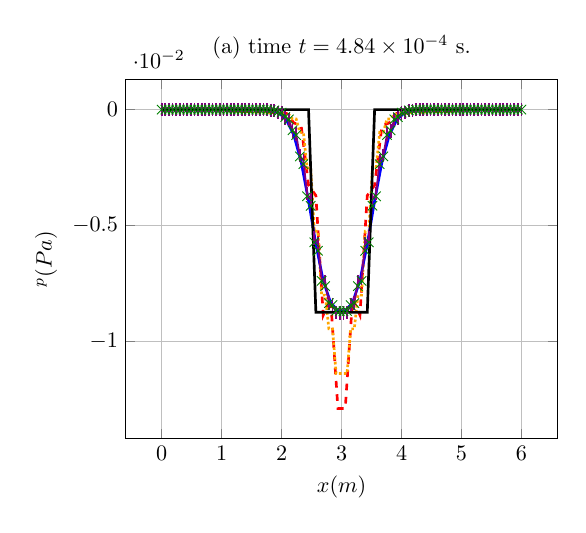
\begin{tikzpicture}[scale=0.8]
\begin{axis}[xlabel=$x (m)$,ylabel=$\eps^p (Pa)$,ymajorgrids=true,xmajorgrids=true,legend pos=outer north east,title={(a) time $t = 4.84\times 10^{-4} $ s.}]
\addplot[Red,very thick,mark=none,dashed,mark size=3pt] coordinates {(0.0,0.0) (0.12244897959183673,0.0) (0.24489795918367346,0.0) (0.36734693877551017,0.0) (0.4897959183673469,0.0) (0.6122448979591837,0.0) (0.7346938775510203,0.0) (0.8571428571428571,0.0) (0.9795918367346939,0.0) (1.1020408163265305,-3.791590211516079e-05) (1.2244897959183674,-7.70866275263142e-05) (1.346938775510204,-8.497586707829323e-05) (1.4693877551020407,-9.030872437715389e-05) (1.5918367346938775,-9.742060457186303e-05) (1.7142857142857142,-0.00011777294632526181) (1.836734693877551,-0.00011877997120884317) (1.9591836734693877,-0.00017229593911894644) (2.0816326530612246,-0.0001625095927714705) (2.204081632653061,-0.0005721718460187986) (2.326530612244898,-0.0006980928227095806) (2.4489795918367347,-0.003255684770391246) (2.571428571428571,-0.003703854150331533) (2.693877551020408,-0.008855536230217072) (2.816326530612245,-0.008134161982050364) (2.9387755102040813,-0.012877303196726952) (3.061224489795918,-0.012877303196726607) (3.183673469387755,-0.008134161982050527) (3.306122448979592,-0.008855536230216924) (3.4285714285714284,-0.00370385415033155) (3.5510204081632653,-0.0032556847703911866) (3.673469387755102,-0.0006980928227095723) (3.7959183673469385,-0.0005721718460187898) (3.9183673469387754,-0.0001625095927714674) (4.040816326530612,-0.00017229593911894956) (4.163265306122449,-0.00011877997120884148) (4.285714285714286,-0.00011777294632525957) (4.408163265306122,-9.74206045718636e-05) (4.530612244897959,-9.030872437715303e-05) (4.653061224489796,-8.497586707829776e-05) (4.775510204081632,-7.708662752631704e-05) (4.8979591836734695,-3.791590211516108e-05) (5.020408163265306,0.0) (5.142857142857142,0.0) (5.26530612244898,0.0) (5.387755102040816,0.0) (5.5102040816326525,0.0) (5.63265306122449,0.0) (5.755102040816326,0.0) (5.877551020408163,0.0) (6.0,0.0) };
\addplot[Orange,very thick,mark=none,densely dotted,mark size=3pt] coordinates {(0.0,0.0) (0.06060606060606061,0.0) (0.12121212121212122,0.0) (0.18181818181818182,0.0) (0.24242424242424243,0.0) (0.30303030303030304,0.0) (0.36363636363636365,0.0) (0.42424242424242425,0.0) (0.48484848484848486,0.0) (0.5454545454545454,0.0) (0.6060606060606061,0.0) (0.6666666666666667,0.0) (0.7272727272727273,0.0) (0.7878787878787878,0.0) (0.8484848484848485,0.0) (0.9090909090909092,0.0) (0.9696969696969697,0.0) (1.0303030303030303,0.0) (1.0909090909090908,-5.189503403045677e-05) (1.1515151515151516,-5.189503403045677e-05) (1.2121212121212122,-7.644801267914517e-05) (1.2727272727272727,-7.644801267914517e-05) (1.3333333333333335,-8.355081233240621e-05) (1.393939393939394,-8.355081233240621e-05) (1.4545454545454546,-8.910062882111044e-05) (1.5151515151515151,-8.910062882111044e-05) (1.5757575757575757,-9.397621508219469e-05) (1.6363636363636365,-9.397621508219469e-05) (1.696969696969697,-0.00010493025008663676) (1.7575757575757576,-0.00010493025008663676) (1.8181818181818183,-0.0001273466612942605) (1.878787878787879,-0.0001273466612942605) (1.9393939393939394,-0.00015215160027546855) (2.0,-0.00015215160027546855) (2.0606060606060606,-0.00020922085638282924) (2.121212121212121,-0.00020922085638282924) (2.1818181818181817,-0.00040275193843327815) (2.2424242424242427,-0.00040275193843327815) (2.303030303030303,-0.0009750544233862026) (2.3636363636363638,-0.0009750544233862026) (2.4242424242424243,-0.0025145499736588055) (2.484848484848485,-0.0025145499736588055) (2.5454545454545454,-0.005244570914165349) (2.606060606060606,-0.005244570914165349) (2.666666666666667,-0.007992615538684102) (2.7272727272727275,-0.007992615538684102) (2.787878787878788,-0.009446048408812087) (2.8484848484848486,-0.009446048408812087) (2.909090909090909,-0.011373543353957122) (2.9696969696969697,-0.011373543353957122) (3.0303030303030303,-0.011373543353957112) (3.090909090909091,-0.011373543353957112) (3.1515151515151514,-0.009446048408812087) (3.2121212121212124,-0.009446048408812087) (3.272727272727273,-0.007992615538684114) (3.3333333333333335,-0.007992615538684114) (3.393939393939394,-0.00524457091416535) (3.4545454545454546,-0.00524457091416535) (3.515151515151515,-0.002514549973658797) (3.5757575757575757,-0.002514549973658797) (3.6363636363636367,-0.0009750544233862052) (3.6969696969696972,-0.0009750544233862052) (3.757575757575758,-0.0004027519384332821) (3.8181818181818183,-0.0004027519384332821) (3.878787878787879,-0.00020922085638282406) (3.9393939393939394,-0.00020922085638282406) (4.0,-0.00015215160027546624) (4.0606060606060606,-0.00015215160027546624) (4.121212121212121,-0.0001273466612942568) (4.181818181818182,-0.0001273466612942568) (4.242424242424242,-0.0001049302500866464) (4.303030303030303,-0.0001049302500866464) (4.363636363636363,-9.397621508218874e-05) (4.424242424242425,-9.397621508218874e-05) (4.484848484848485,-8.910062882111044e-05) (4.545454545454546,-8.910062882111044e-05) (4.606060606060606,-8.35508123324031e-05) (4.666666666666667,-8.35508123324031e-05) (4.7272727272727275,-7.644801267914545e-05) (4.787878787878788,-7.644801267914545e-05) (4.848484848484849,-5.189503403045904e-05) (4.909090909090909,-5.189503403045904e-05) (4.96969696969697,0.0) (5.03030303030303,0.0) (5.090909090909091,0.0) (5.151515151515151,0.0) (5.212121212121212,0.0) (5.2727272727272725,0.0) (5.333333333333334,0.0) (5.3939393939393945,0.0) (5.454545454545455,0.0) (5.515151515151516,0.0) (5.575757575757576,0.0) (5.636363636363637,0.0) (5.696969696969697,0.0) (5.757575757575758,0.0) (5.818181818181818,0.0) (5.878787878787879,0.0) (5.9393939393939394,0.0) (6.0,0.0) };
\addplot[Blue,very thick,mark=none,solid,mark size=3pt] coordinates {(0.0,0.0) (0.12244897959183673,0.0) (0.24489795918367346,0.0) (0.36734693877551017,0.0) (0.4897959183673469,0.0) (0.6122448979591837,-5.222502208891369e-16) (0.7346938775510203,-3.801924841744559e-14) (0.8571428571428571,-1.3141666139875138e-12) (0.9795918367346939,-2.8745591924304055e-11) (1.1020408163265305,-4.464150179000128e-10) (1.2244897959183674,-5.23467841943105e-09) (1.346938775510204,-4.812046858639944e-08) (1.4693877551020407,-3.554036475964955e-07) (1.5918367346938775,-2.1443096765697003e-06) (1.7142857142857142,-1.0689498023182154e-05) (1.836734693877551,-4.436466051051049e-05) (1.9591836734693877,-0.00015404085928397946) (2.0816326530612246,-0.00044873332231471766) (2.204081632653061,-0.0010984305872627827) (2.326530612244898,-0.0022622254025038953) (2.4489795918367347,-0.003929978610103271) (2.571428571428571,-0.005797119893456445) (2.693877551020408,-0.007371043418348148) (2.816326530612245,-0.008310826779347521) (2.9387755102040813,-0.00866523151909913) (3.061224489795918,-0.008665231519099129) (3.183673469387755,-0.008310826779347523) (3.306122448979592,-0.007371043418348151) (3.4285714285714284,-0.0057971198934564485) (3.5510204081632653,-0.003929978610103277) (3.673469387755102,-0.002262225402503906) (3.7959183673469385,-0.0010984305872627934) (3.9183673469387754,-0.0004487333223147267) (4.040816326530612,-0.00015404085928398656) (4.163265306122449,-4.4364660510512195e-05) (4.285714285714286,-1.0689498023171936e-05) (4.408163265306122,-2.144309676557212e-06) (4.530612244897959,-3.554036475865614e-07) (4.653061224489796,-4.8120468574194675e-08) (4.775510204081632,-5.234678408361617e-09) (4.8979591836734695,-4.4641501165571666e-10) (5.020408163265306,-2.874559277579898e-11) (5.142857142857142,-1.314168884640648e-12) (5.26530612244898,-3.802009991237095e-14) (5.387755102040816,-5.242370423816499e-16) (5.5102040816326525,0.0) (5.63265306122449,0.0) (5.755102040816326,0.0) (5.877551020408163,0.0) (6.0,0.0) };
\addplot[Purple,thick,mark=|,solid,mark size=3pt] coordinates {(0.0,0.0) (0.06060606060606061,0.0) (0.12121212121212122,0.0) (0.18181818181818182,0.0) (0.24242424242424243,0.0) (0.30303030303030304,0.0) (0.36363636363636365,0.0) (0.42424242424242425,0.0) (0.48484848484848486,0.0) (0.5454545454545454,0.0) (0.6060606060606061,0.0) (0.6666666666666667,0.0) (0.7272727272727273,0.0) (0.7878787878787878,0.0) (0.8484848484848485,0.0) (0.9090909090909092,0.0) (0.9696969696969697,0.0) (1.0303030303030303,0.0) (1.0909090909090908,0.0) (1.1515151515151516,0.0) (1.2121212121212122,0.0) (1.2727272727272727,0.0) (1.3333333333333335,0.0) (1.393939393939394,-1.0241627792999857e-07) (1.4545454545454546,-2.1818139095136096e-07) (1.5151515151515151,-3.4092713152879763e-07) (1.5757575757575757,-1.326095171369825e-06) (1.6363636363636365,-1.9327126010610944e-06) (1.696969696969697,-7.1982977992651005e-06) (1.7575757575757576,-9.874516857163679e-06) (1.8181818181818183,-3.1832173941879044e-05) (1.878787878787879,-4.148900391485663e-05) (1.9393939393939394,-0.00011652978508307877) (2.0,-0.00014507560252168775) (2.0606060606060606,-0.00035655457656559516) (2.121212121212121,-0.00042570629865757397) (2.1818181818181817,-0.0009162020126129757) (2.2424242424242427,-0.00105240338850247) (2.303030303030303,-0.001980220164065959) (2.3636363636363638,-0.00219491468716409) (2.4242424242424243,-0.0036028496584267246) (2.484848484848485,-0.0038667957458958825) (2.5454545454545454,-0.005536333244818787) (2.606060606060606,-0.005779106783972591) (2.666666666666667,-0.007262784738374422) (2.7272727272727275,-0.007418212916281399) (2.787878787878788,-0.008338349466527659) (2.8484848484848486,-0.008398061506685966) (2.909090909090909,-0.00874932105310645) (2.9696969696969697,-0.00875906579314888) (3.0303030303030303,-0.008759065793148885) (3.090909090909091,-0.008749321053106454) (3.1515151515151514,-0.008398061506685973) (3.2121212121212124,-0.008338349466527662) (3.272727272727273,-0.007418212916281403) (3.3333333333333335,-0.007262784738374426) (3.393939393939394,-0.005779106783972596) (3.4545454545454546,-0.00553633324481879) (3.515151515151515,-0.0038667957458958873) (3.5757575757575757,-0.003602849658426731) (3.6363636363636367,-0.0021949146871640965) (3.6969696969696972,-0.0019802201640659674) (3.757575757575758,-0.0010524033885024758) (3.8181818181818183,-0.0009162020126129829) (3.878787878787879,-0.0004257062986575768) (3.9393939393939394,-0.0003565545765655975) (4.0,-0.00014507560252168976) (4.0606060606060606,-0.00011652978508308132) (4.121212121212121,-4.148900391485918e-05) (4.181818181818182,-3.183217394188217e-05) (4.242424242424242,-9.874516857165381e-06) (4.303030303030303,-7.198297799266805e-06) (4.363636363636363,-1.9327126010608106e-06) (4.424242424242425,-1.3260951713706767e-06) (4.484848484848485,-3.409271315302168e-07) (4.545454545454546,-2.181813909527801e-07) (4.606060606060606,-1.0241627793085007e-07) (4.666666666666667,0.0) (4.7272727272727275,0.0) (4.787878787878788,0.0) (4.848484848484849,0.0) (4.909090909090909,0.0) (4.96969696969697,0.0) (5.03030303030303,0.0) (5.090909090909091,0.0) (5.151515151515151,0.0) (5.212121212121212,0.0) (5.2727272727272725,0.0) (5.333333333333334,0.0) (5.3939393939393945,0.0) (5.454545454545455,0.0) (5.515151515151516,0.0) (5.575757575757576,0.0) (5.636363636363637,0.0) (5.696969696969697,0.0) (5.757575757575758,0.0) (5.818181818181818,0.0) (5.878787878787879,0.0) (5.9393939393939394,0.0) (6.0,0.0) };
\addplot[Green,thin,mark=x,only marks,mark size=3pt] coordinates {(0.0,0.0) (0.06060606060606061,0.0) (0.12121212121212122,0.0) (0.18181818181818182,0.0) (0.24242424242424243,0.0) (0.30303030303030304,0.0) (0.36363636363636365,0.0) (0.42424242424242425,0.0) (0.48484848484848486,0.0) (0.5454545454545454,0.0) (0.6060606060606061,-1.0501770746140254e-17) (0.6666666666666667,-2.639634268624442e-17) (0.7272727272727273,-1.3930456978934152e-15) (0.7878787878787878,-3.0883720942905973e-15) (0.8484848484848485,-7.001587322780064e-14) (0.9090909090909092,-1.4903431846981957e-13) (0.9696969696969697,-2.1913525604066395e-12) (1.0303030303030303,-4.464930579775855e-12) (1.0909090909090908,-4.77809454713549e-11) (1.1515151515151516,-9.306204035168602e-11) (1.2121212121212122,-7.711520115534465e-10) (1.2727272727272727,-1.4337170623597643e-09) (1.3333333333333335,-9.554857790753955e-09) (1.393939393939394,-1.693314060852641e-08) (1.4545454545454546,-9.304669079212916e-08) (1.5151515151515151,-1.5696122348791076e-07) (1.5757575757575757,-7.232737795415378e-07) (1.6363636363636365,-1.1597909965574741e-06) (1.696969696969697,-4.533752320027351e-06) (1.7575757575757576,-6.901910053169727e-06) (1.8181818181818183,-2.3065619941253325e-05) (1.878787878787879,-3.3299321505525566e-05) (1.9393939393939394,-9.55956969570753e-05) (2.0,-0.00013077312616477553) (2.0606060606060606,-0.0003233382771117707) (2.121212121212121,-0.000418991275671649) (2.1818181818181817,-0.000893176596649358) (2.2424242424242427,-0.001096836586440369) (2.303030303030303,-0.0020167583506237943) (2.3636363636363638,-0.0023508767096016648) (2.4242424242424243,-0.003733526786569201) (2.484848484848485,-0.004145706810179733) (2.5454545454545454,-0.005716170295994451) (2.606060606060606,-0.0060844115721184165) (2.666666666666667,-0.007382239901136897) (2.7272727272727275,-0.007606232648853957) (2.787878787878788,-0.008339693841572507) (2.8484848484848486,-0.00842236558917303) (2.909090909090909,-0.008674950007510287) (2.9696969696969697,-0.008688869601046518) (3.0303030303030303,-0.008688869601046518) (3.090909090909091,-0.008674950007510288) (3.1515151515151514,-0.008422365589173027) (3.2121212121212124,-0.008339693841572503) (3.272727272727273,-0.007606232648853953) (3.3333333333333335,-0.0073822399011368965) (3.393939393939394,-0.006084411572118416) (3.4545454545454546,-0.0057161702959944525) (3.515151515151515,-0.004145706810179732) (3.5757575757575757,-0.0037335267865692026) (3.6363636363636367,-0.0023508767096016643) (3.6969696969696972,-0.0020167583506237956) (3.757575757575758,-0.0010968365864403716) (3.8181818181818183,-0.0008931765966493632) (3.878787878787879,-0.0004189912756716515) (3.9393939393939394,-0.0003233382771117741) (4.0,-0.0001307731261647775) (4.0606060606060606,-9.559569695707617e-05) (4.121212121212121,-3.329932150552386e-05) (4.181818181818182,-2.3065619941252752e-05) (4.242424242424242,-6.901910053168876e-06) (4.303030303030303,-4.533752320026216e-06) (4.363636363636363,-1.15979099656088e-06) (4.424242424242425,-7.232737795452277e-07) (4.484848484848485,-1.5696122349358742e-07) (4.545454545454546,-9.304669079865728e-08) (4.606060606060606,-1.6933140614486876e-08) (4.666666666666667,-9.554857795862925e-09) (4.7272727272727275,-1.433717062643596e-09) (4.787878787878788,-7.711520118372781e-10) (4.848484848484849,-9.30620395001911e-11) (4.909090909090909,-4.778094547135489e-11) (4.96969696969697,-4.464928876786005e-12) (5.03030303030303,-2.191354547228132e-12) (5.090909090909091,-1.4903885977608817e-13) (5.151515151515151,-7.002013070242745e-14) (5.212121212121212,-3.0886559259323846e-15) (5.2727272727272725,-1.3902073814755395e-15) (5.333333333333334,-2.923465910412016e-17) (5.3939393939393945,-1.7313730149042037e-17) (5.454545454545455,0.0) (5.515151515151516,0.0) (5.575757575757576,0.0) (5.636363636363637,0.0) (5.696969696969697,0.0) (5.757575757575758,0.0) (5.818181818181818,0.0) (5.878787878787879,0.0) (5.9393939393939394,0.0) (6.0,0.0) };
\addplot[black,very thick,mark=pentagone*,solid,mark size=3pt] coordinates {(0.0,-0.0) (0.12244897959183673,-0.0) (0.24489795918367346,-0.0) (0.36734693877551017,-0.0) (0.4897959183673469,-0.0) (0.6122448979591837,-0.0) (0.7346938775510203,-0.0) (0.8571428571428571,-0.0) (0.9795918367346939,-0.0) (1.1020408163265305,-0.0) (1.2244897959183674,-0.0) (1.346938775510204,-0.0) (1.4693877551020407,-0.0) (1.5918367346938775,-0.0) (1.7142857142857142,-0.0) (1.836734693877551,-0.0) (1.9591836734693877,-0.0) (2.0816326530612246,-0.0) (2.204081632653061,-0.0) (2.326530612244898,-0.0) (2.4489795918367347,-0.0) (2.571428571428571,-0.008728715609439695) (2.693877551020408,-0.008728715609439695) (2.816326530612245,-0.008728715609439695) (2.9387755102040813,-0.008728715609439695) (3.061224489795918,-0.008728715609439695) (3.183673469387755,-0.008728715609439695) (3.306122448979592,-0.008728715609439695) (3.4285714285714284,-0.008728715609439695) (3.5510204081632653,-0.0) (3.673469387755102,-0.0) (3.7959183673469385,-0.0) (3.9183673469387754,-0.0) (4.040816326530612,-0.0) (4.163265306122449,-0.0) (4.285714285714286,-0.0) (4.408163265306122,-0.0) (4.530612244897959,-0.0) (4.653061224489796,-0.0) (4.775510204081632,-0.0) (4.8979591836734695,-0.0) (5.020408163265306,-0.0) (5.142857142857142,-0.0) (5.26530612244898,-0.0) (5.387755102040816,-0.0) (5.5102040816326525,-0.0) (5.63265306122449,-0.0) (5.755102040816326,-0.0) (5.877551020408163,-0.0) (6.0,-0.0) };
%\legend{usl 1ppc,usl 2ppc,dgmpm 1ppc,dgmpm 2ppc,dgmpm 2ppc (RK2),exact}
\end{axis}
\end{tikzpicture}
%%% Local Variables:
%%% mode: latex
%%% TeX-master: "../../mainManuscript"
%%% End:
}
  {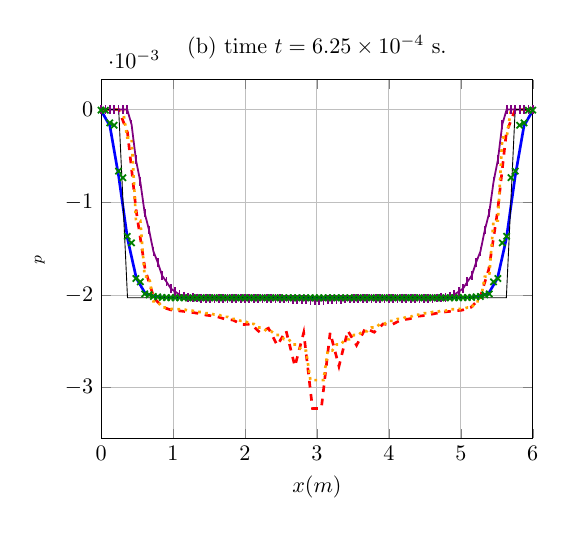
\begin{tikzpicture}[scale=0.8]
\begin{axis}[xlabel=$x (m)$,ylabel=$\eps^p$,ymajorgrids=true,xmajorgrids=true,legend pos=outer north east,title={(b) time $t = 6.25\times 10^{-4} $ s.},xmin=0.,xmax=6.]
\addplot[Red,very thick,mark=none,dashed] coordinates {(0.0,0.0) (0.12244897959183673,0.0) (0.24489795918367346,0.0) (0.36734693877551017,-0.0002478348228815541) (0.4897959183673469,-0.0011004378155012712) (0.6122448979591837,-0.0017260409269248597) (0.7346938775510203,-0.002031865332982762) (0.8571428571428571,-0.002132968518977378) (0.9795918367346939,-0.0021636018350532395) (1.1020408163265305,-0.0021733079916121177) (1.2244897959183674,-0.00218350748748031) (1.346938775510204,-0.002198645448466017) (1.4693877551020407,-0.002218920213241705) (1.5918367346938775,-0.002229697455331896) (1.7142857142857142,-0.002258121963594508) (1.836734693877551,-0.002271799079674154) (1.9591836734693877,-0.002320613632318322) (2.0816326530612246,-0.002313868472160546) (2.204081632653061,-0.0024020122032007017) (2.326530612244898,-0.0023588630990294623) (2.4489795918367347,-0.0025433455597807667) (2.571428571428571,-0.002385435935351422) (2.693877551020408,-0.0027693350417516906) (2.816326530612245,-0.0024065265204776445) (2.9387755102040813,-0.0032250612006492966) (3.061224489795918,-0.0032250612006492524) (3.183673469387755,-0.002406526520477666) (3.306122448979592,-0.0027693350417516823) (3.4285714285714284,-0.0023854359353514295) (3.5510204081632653,-0.0025433455597807628) (3.673469387755102,-0.002358863099029464) (3.7959183673469385,-0.0024020122032006983) (3.9183673469387754,-0.0023138684721605448) (4.040816326530612,-0.002320613632318319) (4.163265306122449,-0.0022717990796741546) (4.285714285714286,-0.0022581219635945077) (4.408163265306122,-0.0022296974553318956) (4.530612244897959,-0.0022189202132417056) (4.653061224489796,-0.0021986454484660173) (4.775510204081632,-0.0021835074874803095) (4.8979591836734695,-0.0021733079916121186) (5.020408163265306,-0.0021636018350532395) (5.142857142857142,-0.002132968518977378) (5.26530612244898,-0.002031865332982763) (5.387755102040816,-0.0017260409269248577) (5.5102040816326525,-0.0011004378155012658) (5.63265306122449,-0.0002478348228815494) (5.755102040816326,0.0) (5.877551020408163,0.0) (6.0,0.0) };
\addplot[Orange,very thick,mark=none,dotted] coordinates {(0.0,0.0) (0.06060606060606061,0.0) (0.12121212121212122,0.0) (0.18181818181818182,0.0) (0.24242424242424243,0.0) (0.30303030303030304,0.0) (0.36363636363636365,-0.0003017574960527518) (0.42424242424242425,-0.0003017574960527518) (0.48484848484848486,-0.0011974917980669022) (0.5454545454545454,-0.0011974917980669022) (0.6060606060606061,-0.0018020040797071544) (0.6666666666666667,-0.0018020040797071544) (0.7272727272727273,-0.002068378033006087) (0.7878787878787878,-0.002068378033006087) (0.8484848484848485,-0.002135941628228986) (0.9090909090909092,-0.002135941628228986) (0.9696969696969697,-0.002150822172714686) (1.0303030303030303,-0.002150822172714686) (1.0909090909090908,-0.002154888242838099) (1.1515151515151516,-0.002154888242838099) (1.2121212121212122,-0.0021700900543690626) (1.2727272727272727,-0.0021700900543690626) (1.3333333333333335,-0.0021843706812353886) (1.393939393939394,-0.0021843706812353886) (1.4545454545454546,-0.0021968313010739355) (1.5151515151515151,-0.0021968313010739355) (1.5757575757575757,-0.0022123334205993417) (1.6363636363636365,-0.0022123334205993417) (1.696969696969697,-0.0022365941606657474) (1.7575757575757576,-0.0022365941606657474) (1.8181818181818183,-0.0022585940891309796) (1.878787878787879,-0.0022585940891309796) (1.9393939393939394,-0.0022798424574663194) (2.0,-0.0022798424574663194) (2.0606060606060606,-0.0023117041253564387) (2.121212121212121,-0.0023117041253564387) (2.1818181818181817,-0.002350782112768782) (2.2424242424242427,-0.002350782112768782) (2.303030303030303,-0.002390940396871615) (2.3636363636363638,-0.002390940396871615) (2.4242424242424243,-0.0024313395034050904) (2.484848484848485,-0.0024313395034050904) (2.5454545454545454,-0.002477563584428502) (2.606060606060606,-0.002477563584428502) (2.666666666666667,-0.0025344573000873694) (2.7272727272727275,-0.0025344573000873694) (2.787878787878788,-0.002600834768573611) (2.8484848484848486,-0.002600834768573611) (2.909090909090909,-0.0029191565184019295) (2.9696969696969697,-0.0029191565184019295) (3.0303030303030303,-0.0029191565184019273) (3.090909090909091,-0.0029191565184019273) (3.1515151515151514,-0.0026008347685736143) (3.2121212121212124,-0.0026008347685736143) (3.272727272727273,-0.002534457300087371) (3.3333333333333335,-0.002534457300087371) (3.393939393939394,-0.0024775635844285025) (3.4545454545454546,-0.0024775635844285025) (3.515151515151515,-0.0024313395034050896) (3.5757575757575757,-0.0024313395034050896) (3.6363636363636367,-0.002390940396871615) (3.6969696969696972,-0.002390940396871615) (3.757575757575758,-0.0023507821127687826) (3.8181818181818183,-0.0023507821127687826) (3.878787878787879,-0.002311704125356438) (3.9393939393939394,-0.002311704125356438) (4.0,-0.0022798424574663172) (4.0606060606060606,-0.0022798424574663172) (4.121212121212121,-0.00225859408913098) (4.181818181818182,-0.00225859408913098) (4.242424242424242,-0.002236594160665746) (4.303030303030303,-0.002236594160665746) (4.363636363636363,-0.0022123334205993426) (4.424242424242425,-0.0022123334205993426) (4.484848484848485,-0.002196831301073935) (4.545454545454546,-0.002196831301073935) (4.606060606060606,-0.0021843706812353886) (4.666666666666667,-0.0021843706812353886) (4.7272727272727275,-0.0021700900543690613) (4.787878787878788,-0.0021700900543690613) (4.848484848484849,-0.0021548882428381) (4.909090909090909,-0.0021548882428381) (4.96969696969697,-0.0021508221727146843) (5.03030303030303,-0.0021508221727146843) (5.090909090909091,-0.002135941628228984) (5.151515151515151,-0.002135941628228984) (5.212121212121212,-0.0020683780330060866) (5.2727272727272725,-0.0020683780330060866) (5.333333333333334,-0.0018020040797071535) (5.3939393939393945,-0.0018020040797071535) (5.454545454545455,-0.0011974917980669003) (5.515151515151516,-0.0011974917980669003) (5.575757575757576,-0.0003017574960527513) (5.636363636363637,-0.0003017574960527513) (5.696969696969697,0.0) (5.757575757575758,0.0) (5.818181818181818,0.0) (5.878787878787879,0.0) (5.9393939393939394,0.0) (6.0,0.0) };
\addplot[Blue,very thick,mark=none,solid] coordinates {(0.0,-8.02367288935203e-06) (0.12244897959183673,-0.00017614426387335805) (0.24489795918367346,-0.0007207542691858686) (0.36734693877551017,-0.0013919930410856215) (0.4897959183673469,-0.001818355598439618) (0.6122448979591837,-0.001981300761387861) (0.7346938775510203,-0.0020125975551096974) (0.8571428571428571,-0.002024874952136019) (0.9795918367346939,-0.0020290867696967987) (1.1020408163265305,-0.002030353909504423) (1.2244897959183674,-0.0020306887880741907) (1.346938775510204,-0.0020307665725143873) (1.4693877551020407,-0.0020307824435747243) (1.5918367346938775,-0.0020307852835259937) (1.7142857142857142,-0.0020307857279245408) (1.836734693877551,-0.0020307857884822454) (1.9591836734693877,-0.00203078579562695) (2.0816326530612246,-0.002030785796351117) (2.204081632653061,-0.0020307857964135248) (2.326530612244898,-0.002030785796418031) (2.4489795918367347,-0.002030785796418302) (2.571428571428571,-0.0020307857964183135) (2.693877551020408,-0.002030785796418313) (2.816326530612245,-0.002030785796418313) (2.9387755102040813,-0.002030785796418314) (3.061224489795918,-0.0020307857964183135) (3.183673469387755,-0.0020307857964183135) (3.306122448979592,-0.0020307857964183126) (3.4285714285714284,-0.0020307857964183113) (3.5510204081632653,-0.0020307857964183005) (3.673469387755102,-0.002030785796418031) (3.7959183673469385,-0.0020307857964135217) (3.9183673469387754,-0.0020307857963511138) (4.040816326530612,-0.002030785795626948) (4.163265306122449,-0.0020307857884822433) (4.285714285714286,-0.0020307857279245403) (4.408163265306122,-0.0020307852835259915) (4.530612244897959,-0.0020307824435747226) (4.653061224489796,-0.0020307665725143842) (4.775510204081632,-0.002030688788074188) (4.8979591836734695,-0.0020303539095044196) (5.020408163265306,-0.0020290867696967953) (5.142857142857142,-0.0020248749521360144) (5.26530612244898,-0.0020125975551096966) (5.387755102040816,-0.0019813007613878565) (5.5102040816326525,-0.0018183555984396154) (5.63265306122449,-0.0013919930410856195) (5.755102040816326,-0.0007207542691858678) (5.877551020408163,-0.0001761442638733595) (6.0,-8.023672889353243e-06) };
\addplot[Purple,thick,mark=|,solid] coordinates {(0.0,0.0) (0.06060606060606061,0.0) (0.12121212121212122,0.0) (0.18181818181818182,0.0) (0.24242424242424243,0.0) (0.30303030303030304,0.0) (0.36363636363636365,0.0) (0.42424242424242425,-0.00016170662401525856) (0.48484848484848486,-0.0005417551163059964) (0.5454545454545454,-0.0007797468469340016) (0.6060606060606061,-0.0011158014314235371) (0.6666666666666667,-0.0012988809897543044) (0.7272727272727273,-0.0015295338295444575) (0.7878787878787878,-0.0016494591967999013) (0.8484848484848485,-0.001791241808636007) (0.9090909090909092,-0.001858139654558482) (0.9696969696969697,-0.0019313228858157505) (1.0303030303030303,-0.001963941276484258) (1.0909090909090908,-0.00199709045414516) (1.1515151515151516,-0.0020110149368315873) (1.2121212121212122,-0.0020240838020015965) (1.2727272727272727,-0.002029112099138213) (1.3333333333333335,-0.002033444493020763) (1.393939393939394,-0.0020349375209240046) (1.4545454545454546,-0.0020360626617364976) (1.5151515151515151,-0.002036427946256999) (1.5757575757575757,-0.0020366368397527423) (1.6363636363636365,-0.002036698090585699) (1.696969696969697,-0.0020368405580576125) (1.7575757575757576,-0.0020369810286138333) (1.8181818181818183,-0.0020373219984231514) (1.878787878787879,-0.002037585653215558) (1.9393939393939394,-0.002037962720224221) (2.0,-0.002038127417033818) (2.0606060606060606,-0.0020383611759408468) (2.121212121212121,-0.002038518677096413) (2.1818181818181817,-0.0020388624173375575) (2.2424242424242427,-0.002039197521601926) (2.303030303030303,-0.0020400227446406255) (2.3636363636363638,-0.0020406530704546125) (2.4242424242424243,-0.0020416018700111314) (2.484848484848485,-0.00204214484166886) (2.5454545454545454,-0.002043028167195094) (2.606060606060606,-0.0020436145435565973) (2.666666666666667,-0.0020449363268448036) (2.7272727272727275,-0.0020459859423928813) (2.787878787878788,-0.002048543419164452) (2.8484848484848486,-0.002051015793534283) (2.909090909090909,-0.0020569476212071243) (2.9696969696969697,-0.0020621904992435833) (3.0303030303030303,-0.0020621904992435824) (3.090909090909091,-0.002056947621207125) (3.1515151515151514,-0.0020510157935342823) (3.2121212121212124,-0.002048543419164453) (3.272727272727273,-0.0020459859423928826) (3.3333333333333335,-0.0020449363268448045) (3.393939393939394,-0.0020436145435565965) (3.4545454545454546,-0.002043028167195095) (3.515151515151515,-0.0020421448416688593) (3.5757575757575757,-0.002041601870011131) (3.6363636363636367,-0.00204065307045461) (3.6969696969696972,-0.0020400227446406246) (3.757575757575758,-0.0020391975216019266) (3.8181818181818183,-0.002038862417337557) (3.878787878787879,-0.002038518677096414) (3.9393939393939394,-0.0020383611759408476) (4.0,-0.002038127417033818) (4.0606060606060606,-0.002037962720224222) (4.121212121212121,-0.0020375856532155604) (4.181818181818182,-0.002037321998423153) (4.242424242424242,-0.002036981028613838) (4.303030303030303,-0.0020368405580576134) (4.363636363636363,-0.002036698090585699) (4.424242424242425,-0.0020366368397527414) (4.484848484848485,-0.002036427946257001) (4.545454545454546,-0.0020360626617365023) (4.606060606060606,-0.0020349375209240063) (4.666666666666667,-0.002033444493020765) (4.7272727272727275,-0.002029112099138214) (4.787878787878788,-0.0020240838020015987) (4.848484848484849,-0.00201101493683159) (4.909090909090909,-0.0019970904541451633) (4.96969696969697,-0.001963941276484259) (5.03030303030303,-0.0019313228858157542) (5.090909090909091,-0.0018581396545584844) (5.151515151515151,-0.0017912418086360104) (5.212121212121212,-0.001649459196799904) (5.2727272727272725,-0.001529533829544461) (5.333333333333334,-0.0012988809897543081) (5.3939393939393945,-0.0011158014314235415) (5.454545454545455,-0.000779746846934003) (5.515151515151516,-0.0005417551163059989) (5.575757575757576,-0.00016170662401526048) (5.636363636363637,0.0) (5.696969696969697,0.0) (5.757575757575758,0.0) (5.818181818181818,0.0) (5.878787878787879,0.0) (5.9393939393939394,0.0) (6.0,0.0) };
\addplot[Green,thick,mark=x,only marks] coordinates {(0.0,-5.335532070735344e-06) (0.06060606060606061,-6.7706518097916305e-06) (0.12121212121212122,-0.00014296272370405532) (0.18181818181818182,-0.00016863154669993438) (0.24242424242424243,-0.0006638300086644545) (0.30303030303030304,-0.000734378934081307) (0.36363636363636365,-0.0013668887954266346) (0.42424242424242425,-0.0014381987584863236) (0.48484848484848486,-0.0018228537169639558) (0.5454545454545454,-0.0018582326659348394) (0.6060606060606061,-0.0019882143939252963) (0.6666666666666667,-0.001998178050264291) (0.7272727272727273,-0.0020167573045254297) (0.7878787878787878,-0.0020205950613102187) (0.8484848484848485,-0.0020268204253525244) (0.9090909090909092,-0.0020280653889615647) (0.9696969696969697,-0.0020298272803462047) (1.0303030303030303,-0.002030167668233374) (1.0909090909090908,-0.0020305882754214715) (1.1515151515151516,-0.0020306665744077384) (1.2121212121212122,-0.002030751197289206) (1.2727272727272727,-0.002030766353237554) (1.3333333333333335,-0.0020307803579508853) (1.393939393939394,-0.002030782732084688) (1.4545454545454546,-0.002030784516510227) (1.5151515151515151,-0.0020307847942330386) (1.5757575757575757,-0.0020307855174271218) (1.6363636363636365,-0.0020307856825908114) (1.696969696969697,-0.002030785724102555) (1.7575757575757576,-0.0020307858759962597) (1.8181818181818183,-0.002030785951180978) (1.878787878787879,-0.0020307860418172555) (1.9393939393939394,-0.002030786134808208) (2.0,-0.002030786322147464) (2.0606060606060606,-0.0020307863445982147) (2.121212121212121,-0.0020307866728231407) (2.1818181818181817,-0.0020307867744393435) (2.2424242424242427,-0.002030787015486384) (2.303030303030303,-0.002030787409711756) (2.3636363636363638,-0.0020307883320914285) (2.4242424242424243,-0.0020307890300132712) (2.484848484848485,-0.0020307901307202374) (2.5454545454545454,-0.002030792281554236) (2.606060606060606,-0.002030795453324907) (2.666666666666667,-0.0020307979071881566) (2.7272727272727275,-0.0020308065650964362) (2.787878787878788,-0.002030816863285245) (2.8484848484848486,-0.0020308137021312345) (2.909090909090909,-0.0020308908094497746) (2.9696969696969697,-0.002031166801141057) (3.0303030303030303,-0.0020311668011410568) (3.090909090909091,-0.002030890809449775) (3.1515151515151514,-0.002030813702131235) (3.2121212121212124,-0.002030816863285247) (3.272727272727273,-0.002030806565096435) (3.3333333333333335,-0.0020307979071881553) (3.393939393939394,-0.0020307954533249043) (3.4545454545454546,-0.0020307922815542352) (3.515151515151515,-0.0020307901307202374) (3.5757575757575757,-0.0020307890300132712) (3.6363636363636367,-0.00203078833209143) (3.6969696969696972,-0.002030787409711759) (3.757575757575758,-0.0020307870154863874) (3.8181818181818183,-0.002030786774439345) (3.878787878787879,-0.0020307866728231446) (3.9393939393939394,-0.0020307863445982177) (4.0,-0.0020307863221474677) (4.0606060606060606,-0.002030786134808209) (4.121212121212121,-0.002030786041817254) (4.181818181818182,-0.0020307859511809767) (4.242424242424242,-0.0020307858759962614) (4.303030303030303,-0.002030785724102557) (4.363636363636363,-0.0020307856825908114) (4.424242424242425,-0.002030785517427123) (4.484848484848485,-0.00203078479423304) (4.545454545454546,-0.0020307845165102286) (4.606060606060606,-0.0020307827320846885) (4.666666666666667,-0.002030780357950887) (4.7272727272727275,-0.002030766353237556) (4.787878787878788,-0.0020307511972892083) (4.848484848484849,-0.00203066657440774) (4.909090909090909,-0.0020305882754214715) (4.96969696969697,-0.002030167668233377) (5.03030303030303,-0.002029827280346208) (5.090909090909091,-0.0020280653889615655) (5.151515151515151,-0.002026820425352526) (5.212121212121212,-0.002020595061310217) (5.2727272727272725,-0.0020167573045254293) (5.333333333333334,-0.001998178050264289) (5.3939393939393945,-0.001988214393925294) (5.454545454545455,-0.001858232665934836) (5.515151515151516,-0.0018228537169639517) (5.575757575757576,-0.0014381987584863212) (5.636363636363637,-0.0013668887954266316) (5.696969696969697,-0.0007343789340813044) (5.757575757575758,-0.0006638300086644511) (5.818181818181818,-0.00016863154669993243) (5.878787878787879,-0.0001429627237040512) (5.9393939393939394,-6.770651809786295e-06) (6.0,-5.335532070731949e-06) };
\addplot[black,thin,mark=none,solid] coordinates {(0.0,-0.0) (0.12244897959183673,-0.0) (0.24489795918367346,-0.0) (0.36734693877551017,-0.002030785796418313) (0.4897959183673469,-0.002030785796418313) (0.6122448979591837,-0.002030785796418313) (0.7346938775510203,-0.002030785796418313) (0.8571428571428571,-0.002030785796418313) (0.9795918367346939,-0.002030785796418313) (1.1020408163265305,-0.002030785796418313) (1.2244897959183674,-0.002030785796418313) (1.346938775510204,-0.002030785796418313) (1.4693877551020407,-0.002030785796418313) (1.5918367346938775,-0.002030785796418313) (1.7142857142857142,-0.002030785796418313) (1.836734693877551,-0.002030785796418313) (1.9591836734693877,-0.002030785796418313) (2.0816326530612246,-0.002030785796418313) (2.204081632653061,-0.002030785796418313) (2.326530612244898,-0.002030785796418313) (2.4489795918367347,-0.002030785796418313) (2.571428571428571,-0.002030785796418313) (2.693877551020408,-0.002030785796418313) (2.816326530612245,-0.002030785796418313) (2.9387755102040813,-0.002030785796418313) (3.061224489795918,-0.002030785796418313) (3.183673469387755,-0.002030785796418313) (3.306122448979592,-0.002030785796418313) (3.4285714285714284,-0.002030785796418313) (3.5510204081632653,-0.002030785796418313) (3.673469387755102,-0.002030785796418313) (3.7959183673469385,-0.002030785796418313) (3.9183673469387754,-0.002030785796418313) (4.040816326530612,-0.002030785796418313) (4.163265306122449,-0.002030785796418313) (4.285714285714286,-0.002030785796418313) (4.408163265306122,-0.002030785796418313) (4.530612244897959,-0.002030785796418313) (4.653061224489796,-0.002030785796418313) (4.775510204081632,-0.002030785796418313) (4.8979591836734695,-0.002030785796418313) (5.020408163265306,-0.002030785796418313) (5.142857142857142,-0.002030785796418313) (5.26530612244898,-0.002030785796418313) (5.387755102040816,-0.002030785796418313) (5.5102040816326525,-0.002030785796418313) (5.63265306122449,-0.002030785796418313) (5.755102040816326,-0.0) (5.877551020408163,-0.0) (6.0,-0.0) };
%\legend{usl 1ppc,usl 2ppc,dgmpm 1ppc,dgmpm 2ppc,dgmpm 2ppc (RK2),exact}
\end{axis}
\end{tikzpicture}
%%% Local Variables:
%%% mode: latex
%%% TeX-master: "../../mainManuscript"
%%% End:
}
  {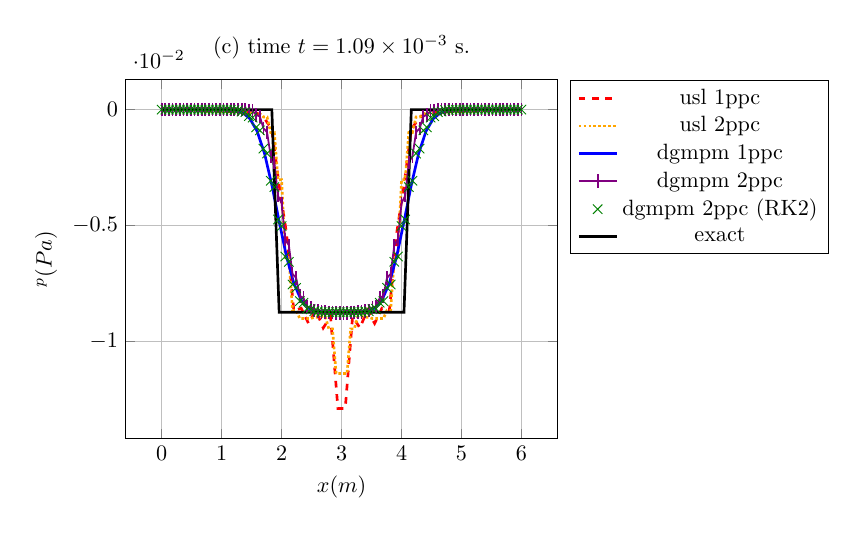
\begin{tikzpicture}[scale=0.8]
\begin{axis}[xlabel=$x (m)$,ylabel=$\eps^p (Pa)$,ymajorgrids=true,xmajorgrids=true,legend pos=outer north east,title={(c) time $t = 1.09\times 10^{-3} $ s.}]
\addplot[Red,very thick,mark=none,dashed,mark size=3pt] coordinates {(0.0,0.0) (0.12244897959183673,0.0) (0.24489795918367346,0.0) (0.36734693877551017,0.0) (0.4897959183673469,0.0) (0.6122448979591837,-3.577487902203997e-05) (0.7346938775510203,-6.306588245633642e-05) (0.8571428571428571,-6.949496312549484e-05) (0.9795918367346939,-8.005219978840035e-05) (1.1020408163265305,-9.009475914811774e-05) (1.2244897959183674,-9.858795071160678e-05) (1.346938775510204,-0.00010648019894997112) (1.4693877551020407,-0.00013090237763271645) (1.5918367346938775,-0.00015585484694440393) (1.7142857142857142,-0.00037807434010367157) (1.836734693877551,-0.0008542508721889013) (1.9591836734693877,-0.003265580636192999) (2.0816326530612246,-0.005332403663610279) (2.204081632653061,-0.008685547798871193) (2.326530612244898,-0.008557827562005196) (2.4489795918367347,-0.009212270529983918) (2.571428571428571,-0.008640321746270047) (2.693877551020408,-0.009408157524816411) (2.816326530612245,-0.008914806029937274) (2.9387755102040813,-0.012877303196726952) (3.061224489795918,-0.012877303196726607) (3.183673469387755,-0.008914806029937388) (3.306122448979592,-0.00940815752481628) (3.4285714285714284,-0.008640321746270135) (3.5510204081632653,-0.009212270529983827) (3.673469387755102,-0.008557827562005267) (3.7959183673469385,-0.008685547798871113) (3.9183673469387754,-0.005332403663610266) (4.040816326530612,-0.003265580636192934) (4.163265306122449,-0.0008542508721888987) (4.285714285714286,-0.00037807434010366447) (4.408163265306122,-0.00015585484694441217) (4.530612244897959,-0.00013090237763272187) (4.653061224489796,-0.00010648019894998299) (4.775510204081632,-9.858795071160708e-05) (4.8979591836734695,-9.00947591481104e-05) (5.020408163265306,-8.005219978840008e-05) (5.142857142857142,-6.949496312550109e-05) (5.26530612244898,-6.306588245633955e-05) (5.387755102040816,-3.5774879022040825e-05) (5.5102040816326525,0.0) (5.63265306122449,0.0) (5.755102040816326,0.0) (5.877551020408163,0.0) (6.0,0.0) };
\addplot[Orange,very thick,mark=none,densely dotted,mark size=3pt] coordinates {(0.0,0.0) (0.06060606060606061,0.0) (0.12121212121212122,0.0) (0.18181818181818182,0.0) (0.24242424242424243,0.0) (0.30303030303030304,0.0) (0.36363636363636365,0.0) (0.42424242424242425,0.0) (0.48484848484848486,-1.3923950014088835e-06) (0.5454545454545454,-1.3923950014088835e-06) (0.6060606060606061,-4.802593874190819e-05) (0.6666666666666667,-4.802593874190819e-05) (0.7272727272727273,-6.41910410194221e-05) (0.7878787878787878,-6.41910410194221e-05) (0.8484848484848485,-6.859024545017706e-05) (0.9090909090909092,-6.859024545017706e-05) (0.9696969696969697,-7.288774581652991e-05) (1.0303030303030303,-7.288774581652991e-05) (1.0909090909090908,-8.507726423586093e-05) (1.1515151515151516,-8.507726423586093e-05) (1.2121212121212122,-9.691077127878779e-05) (1.2727272727272727,-9.691077127878779e-05) (1.3333333333333335,-0.00010711649363712468) (1.393939393939394,-0.00010711649363712468) (1.4545454545454546,-0.00012487268940087668) (1.5151515151515151,-0.00012487268940087668) (1.5757575757575757,-0.00016846150368530778) (1.6363636363636365,-0.00016846150368530778) (1.696969696969697,-0.00032141238951341054) (1.7575757575757576,-0.00032141238951341054) (1.8181818181818183,-0.0009863835722303473) (1.878787878787879,-0.0009863835722303473) (1.9393939393939394,-0.003025063907376677) (2.0,-0.003025063907376677) (2.0606060606060606,-0.006366348809033719) (2.121212121212121,-0.006366348809033719) (2.1818181818181817,-0.008647239978151484) (2.2424242424242427,-0.008647239978151484) (2.303030303030303,-0.009001860585213824) (2.3636363636363638,-0.009001860585213824) (2.4242424242424243,-0.009001507335175213) (2.484848484848485,-0.009001507335175213) (2.5454545454545454,-0.008949274888554966) (2.606060606060606,-0.008949274888554966) (2.666666666666667,-0.00891581762874243) (2.7272727272727275,-0.00891581762874243) (2.787878787878788,-0.00944634271615033) (2.8484848484848486,-0.00944634271615033) (2.909090909090909,-0.011373543353957122) (2.9696969696969697,-0.011373543353957122) (3.0303030303030303,-0.011373543353957112) (3.090909090909091,-0.011373543353957112) (3.1515151515151514,-0.009446342716150326) (3.2121212121212124,-0.009446342716150326) (3.272727272727273,-0.00891581762874244) (3.3333333333333335,-0.00891581762874244) (3.393939393939394,-0.008949274888554966) (3.4545454545454546,-0.008949274888554966) (3.515151515151515,-0.009001507335175215) (3.5757575757575757,-0.009001507335175215) (3.6363636363636367,-0.009001860585213826) (3.6969696969696972,-0.009001860585213826) (3.757575757575758,-0.008647239978151493) (3.8181818181818183,-0.008647239978151493) (3.878787878787879,-0.006366348809033716) (3.9393939393939394,-0.006366348809033716) (4.0,-0.003025063907376669) (4.0606060606060606,-0.003025063907376669) (4.121212121212121,-0.0009863835722303564) (4.181818181818182,-0.0009863835722303564) (4.242424242424242,-0.00032141238951339976) (4.303030303030303,-0.00032141238951339976) (4.363636363636363,-0.00016846150368530894) (4.424242424242425,-0.00016846150368530894) (4.484848484848485,-0.00012487268940087758) (4.545454545454546,-0.00012487268940087758) (4.606060606060606,-0.00010711649363712272) (4.666666666666667,-0.00010711649363712272) (4.7272727272727275,-9.691077127878893e-05) (4.787878787878788,-9.691077127878893e-05) (4.848484848484849,-8.507726423586494e-05) (4.909090909090909,-8.507726423586494e-05) (4.96969696969697,-7.288774581652709e-05) (5.03030303030303,-7.288774581652709e-05) (5.090909090909091,-6.859024545017819e-05) (5.151515151515151,-6.859024545017819e-05) (5.212121212121212,-6.419104101942352e-05) (5.2727272727272725,-6.419104101942352e-05) (5.333333333333334,-4.8025938741907344e-05) (5.3939393939393945,-4.8025938741907344e-05) (5.454545454545455,-1.3923950014085998e-06) (5.515151515151516,-1.3923950014085998e-06) (5.575757575757576,0.0) (5.636363636363637,0.0) (5.696969696969697,0.0) (5.757575757575758,0.0) (5.818181818181818,0.0) (5.878787878787879,0.0) (5.9393939393939394,0.0) (6.0,0.0) };
\addplot[Blue,very thick,mark=none,solid,mark size=3pt] coordinates {(0.0,-5.676632835751488e-19) (0.12244897959183673,-2.3898624238513766e-16) (0.24489795918367346,-3.735990751357306e-14) (0.36734693877551017,-2.3089144911084856e-12) (0.4897959183673469,-7.596762237094698e-11) (0.6122448979591837,-1.5415975357804979e-09) (0.7346938775510203,-2.1087029002110162e-08) (0.8571428571428571,-2.0628580472526095e-07) (0.9795918367346939,-1.5051975779320511e-06) (1.1020408163265305,-8.452232526292688e-06) (1.2244897959183674,-3.741900938747327e-05) (1.346938775510204,-0.00013315210803806102) (1.4693877551020407,-0.00038701776930482674) (1.5918367346938775,-0.0009319386970470464) (1.7142857142857142,-0.0018842066770200564) (1.836734693877551,-0.0032431409441831516) (1.9591836734693877,-0.004827293901207316) (2.0816326530612246,-0.00633202118341673) (2.204081632653061,-0.007489880430691718) (2.326530612244898,-0.008204526972019307) (2.4489795918367347,-0.008552921390073501) (2.571428571428571,-0.008674876019514461) (2.693877551020408,-0.008716486656783273) (2.816326530612245,-0.008726887116624966) (2.9387755102040813,-0.008728580772745199) (3.061224489795918,-0.008728580772745199) (3.183673469387755,-0.008726887116624966) (3.306122448979592,-0.00871648665678328) (3.4285714285714284,-0.008674876019514466) (3.5510204081632653,-0.008552921390073511) (3.673469387755102,-0.008204526972019318) (3.7959183673469385,-0.007489880430691721) (3.9183673469387754,-0.00633202118341673) (4.040816326530612,-0.0048272939012073204) (4.163265306122449,-0.0032431409441831525) (4.285714285714286,-0.001884206677020053) (4.408163265306122,-0.0009319386970470392) (4.530612244897959,-0.0003870177693048181) (4.653061224489796,-0.0001331521080380519) (4.775510204081632,-3.7419009387462476e-05) (4.8979591836734695,-8.452232526284741e-06) (5.020408163265306,-1.5051975779246716e-06) (5.142857142857142,-2.0628580471617835e-07) (5.26530612244898,-2.1087028991608393e-08) (5.387755102040816,-1.5415975312391917e-09) (5.5102040816326525,-7.596762123562041e-11) (5.63265306122449,-2.308913923445202e-12) (5.755102040816326,-3.7358772187005907e-14) (5.877551020408163,-2.4097306387765065e-16) (6.0,-8.514949253627233e-19) };
\addplot[Purple,thick,mark=|,solid,mark size=3pt] coordinates {(0.0,0.0) (0.06060606060606061,0.0) (0.12121212121212122,0.0) (0.18181818181818182,0.0) (0.24242424242424243,0.0) (0.30303030303030304,0.0) (0.36363636363636365,0.0) (0.42424242424242425,0.0) (0.48484848484848486,0.0) (0.5454545454545454,0.0) (0.6060606060606061,0.0) (0.6666666666666667,0.0) (0.7272727272727273,0.0) (0.7878787878787878,0.0) (0.8484848484848485,0.0) (0.9090909090909092,0.0) (0.9696969696969697,0.0) (1.0303030303030303,0.0) (1.0909090909090908,0.0) (1.1515151515151516,-4.1375394533929374e-08) (1.2121212121212122,-1.6766275644359134e-07) (1.2727272727272727,-3.6899460485265364e-07) (1.3333333333333335,-3.7730684118324803e-06) (1.393939393939394,-6.566829345463855e-06) (1.4545454545454546,-3.9533489461271815e-05) (1.5151515151515151,-5.787873091723124e-05) (1.5757575757575757,-0.0002274525995650831) (1.6363636363636365,-0.00029636567097843057) (1.696969696969697,-0.0008043486101741406) (1.7575757575757576,-0.0009756904136278646) (1.8181818181818183,-0.002007506978689405) (1.878787878787879,-0.0022778320644552875) (1.9393939393939394,-0.0037101075201987303) (2.0,-0.004034858131037031) (2.0606060606060606,-0.005583330117719787) (2.121212121212121,-0.005852176347303774) (2.1818181818181817,-0.007081628136433296) (2.2424242424242427,-0.007249585758095964) (2.303030303030303,-0.008025296353006806) (2.3636363636363638,-0.008110184081085586) (2.4242424242424243,-0.008492622343293309) (2.484848484848485,-0.008525512701242518) (2.5454545454545454,-0.008671015536515168) (2.606060606060606,-0.008680086368368912) (2.666666666666667,-0.008720691408181637) (2.7272727272727275,-0.008722186625565662) (2.787878787878788,-0.00872959098319658) (2.8484848484848486,-0.008729715721981647) (2.909090909090909,-0.008758042662148493) (2.9696969696969697,-0.008762227333878615) (3.0303030303030303,-0.008762227333878615) (3.090909090909091,-0.008758042662148495) (3.1515151515151514,-0.008729715721981645) (3.2121212121212124,-0.008729590983196582) (3.272727272727273,-0.008722186625565662) (3.3333333333333335,-0.008720691408181639) (3.393939393939394,-0.00868008636836891) (3.4545454545454546,-0.008671015536515165) (3.515151515151515,-0.008525512701242514) (3.5757575757575757,-0.008492622343293309) (3.6363636363636367,-0.00811018408108559) (3.6969696969696972,-0.008025296353006812) (3.757575757575758,-0.007249585758095969) (3.8181818181818183,-0.0070816281364333026) (3.878787878787879,-0.005852176347303775) (3.9393939393939394,-0.005583330117719789) (4.0,-0.0040348581310370385) (4.0606060606060606,-0.0037101075201987394) (4.121212121212121,-0.0022778320644552983) (4.181818181818182,-0.002007506978689416) (4.242424242424242,-0.0009756904136278739) (4.303030303030303,-0.0008043486101741499) (4.363636363636363,-0.00029636567097843854) (4.424242424242425,-0.00022745259956509018) (4.484848484848485,-5.787873091724344e-05) (4.545454545454546,-3.9533489461283464e-05) (4.606060606060606,-6.566829345470383e-06) (4.666666666666667,-3.773068411838724e-06) (4.7272727272727275,-3.68994604853789e-07) (4.787878787878788,-1.6766275644359137e-07) (4.848484848484849,-4.1375394533929374e-08) (4.909090909090909,0.0) (4.96969696969697,0.0) (5.03030303030303,0.0) (5.090909090909091,0.0) (5.151515151515151,0.0) (5.212121212121212,0.0) (5.2727272727272725,0.0) (5.333333333333334,0.0) (5.3939393939393945,0.0) (5.454545454545455,0.0) (5.515151515151516,0.0) (5.575757575757576,0.0) (5.636363636363637,0.0) (5.696969696969697,0.0) (5.757575757575758,0.0) (5.818181818181818,0.0) (5.878787878787879,0.0) (5.9393939393939394,0.0) (6.0,0.0) };
\addplot[Green,thin,mark=x,only marks,mark size=3pt] coordinates {(0.0,-5.676632835751488e-19) (0.06060606060606061,0.0) (0.12121212121212122,-5.960464477539063e-18) (0.18181818181818182,-8.231117611839657e-18) (0.24242424242424243,-1.2593609946114675e-15) (0.30303030303030304,-2.566973368326823e-15) (0.36363636363636365,-1.2795357477097285e-13) (0.42424242424242425,-2.4569800921848845e-13) (0.48484848484848486,-6.614250512350173e-12) (0.5454545454545454,-1.1978970822833834e-11) (0.6060606060606061,-2.014539040270306e-10) (0.6666666666666667,-3.4473041437921067e-10) (0.7272727272727273,-3.958928195919309e-09) (0.7878787878787878,-6.412620588143667e-09) (0.8484848484848485,-5.3364499986455554e-08) (0.9090909090909092,-8.197237874269486e-08) (0.9696969696969697,-5.155914888793514e-07) (1.0303030303030303,-7.524956608332339e-07) (1.0909090909090908,-3.6911086009462675e-06) (1.1515151515151516,-5.128586973845675e-06) (1.2121212121212122,-2.0096823934549662e-05) (1.2727272727272727,-2.6639006500208663e-05) (1.3333333333333335,-8.500574414884647e-05) (1.393939393939394,-0.00010773647495164076) (1.4545454545454546,-0.00028442785366869175) (1.5151515151515151,-0.0003455251868600774) (1.5757575757575757,-0.0007651640013258602) (1.6363636363636365,-0.0008934272034897002) (1.696969696969697,-0.0016811593270009762) (1.7575757575757576,-0.001892798143971582) (1.8181818181818183,-0.0030669939640570066) (1.878787878787879,-0.0033423564247713746) (1.9393939393939394,-0.004734809703010922) (2.0,-0.005017334536365495) (2.0606060606060606,-0.006329679309076545) (2.121212121212121,-0.006557472732041174) (2.1818181818181817,-0.007536143497329047) (2.2424242424242427,-0.007679356454328646) (2.303030303030303,-0.00825193835878759) (2.3636363636363638,-0.008321206280476908) (2.4242424242424243,-0.008580337649446788) (2.484848484848485,-0.008605558443364046) (2.5454545454545454,-0.008686715531944143) (2.606060606060606,-0.008694798692719908) (2.666666666666667,-0.008720028673057422) (2.7272727272727275,-0.008721895117205144) (2.787878787878788,-0.008727550668862797) (2.8484848484848486,-0.008727826804119215) (2.909090909090909,-0.00872863974231939) (2.9696969696969697,-0.008728659383864157) (3.0303030303030303,-0.008728659383864159) (3.090909090909091,-0.008728639742319392) (3.1515151515151514,-0.008727826804119217) (3.2121212121212124,-0.008727550668862803) (3.272727272727273,-0.008721895117205145) (3.3333333333333335,-0.008720028673057423) (3.393939393939394,-0.008694798692719906) (3.4545454545454546,-0.008686715531944143) (3.515151515151515,-0.008605558443364044) (3.5757575757575757,-0.008580337649446788) (3.6363636363636367,-0.008321206280476912) (3.6969696969696972,-0.008251938358787594) (3.757575757575758,-0.007679356454328649) (3.8181818181818183,-0.0075361434973290516) (3.878787878787879,-0.006557472732041174) (3.9393939393939394,-0.006329679309076547) (4.0,-0.005017334536365494) (4.0606060606060606,-0.004734809703010924) (4.121212121212121,-0.0033423564247713777) (4.181818181818182,-0.0030669939640570088) (4.242424242424242,-0.0018927981439715827) (4.303030303030303,-0.001681159327000978) (4.363636363636363,-0.0008934272034897071) (4.424242424242425,-0.0007651640013258641) (4.484848484848485,-0.00034552518686008227) (4.545454545454546,-0.00028442785366869516) (4.606060606060606,-0.00010773647495164786) (4.666666666666667,-8.500574414885329e-05) (4.7272727272727275,-2.6639006500214904e-05) (4.787878787878788,-2.009682393455562e-05) (4.848484848484849,-5.1285869738558925e-06) (4.909090909090909,-3.6911086009562015e-06) (4.96969696969697,-7.524956608437356e-07) (5.03030303030303,-5.155914888895694e-07) (5.090909090909091,-8.197237874439784e-08) (5.151515151515151,-5.336449998730705e-08) (5.212121212121212,-6.412620592684973e-09) (5.2727272727272725,-3.958928200460616e-09) (5.333333333333334,-3.4473041579836887e-10) (5.3939393939393945,-2.014539034593673e-10) (5.454545454545455,-1.1978968552180698e-11) (5.515151515151516,-6.614249377023606e-12) (5.575757575757576,-2.45694603238787e-13) (5.636363636363637,-1.2795045262291317e-13) (5.696969696969697,-2.566405705043248e-15) (5.757575757575758,-1.2633346375964938e-15) (5.818181818181818,-1.2772423880440849e-17) (5.878787878787879,-6.528127761114212e-18) (5.9393939393939394,0.0) (6.0,0.0) };
\addplot[black,very thick,mark=pentagone*,solid,mark size=3pt] coordinates {(0.0,-0.0) (0.12244897959183673,-0.0) (0.24489795918367346,-0.0) (0.36734693877551017,-0.0) (0.4897959183673469,-0.0) (0.6122448979591837,-0.0) (0.7346938775510203,-0.0) (0.8571428571428571,-0.0) (0.9795918367346939,-0.0) (1.1020408163265305,-0.0) (1.2244897959183674,-0.0) (1.346938775510204,-0.0) (1.4693877551020407,-0.0) (1.5918367346938775,-0.0) (1.7142857142857142,-0.0) (1.836734693877551,-0.0) (1.9591836734693877,-0.008728715609439695) (2.0816326530612246,-0.008728715609439695) (2.204081632653061,-0.008728715609439695) (2.326530612244898,-0.008728715609439695) (2.4489795918367347,-0.008728715609439695) (2.571428571428571,-0.008728715609439695) (2.693877551020408,-0.008728715609439695) (2.816326530612245,-0.008728715609439695) (2.9387755102040813,-0.008728715609439695) (3.061224489795918,-0.008728715609439695) (3.183673469387755,-0.008728715609439695) (3.306122448979592,-0.008728715609439695) (3.4285714285714284,-0.008728715609439695) (3.5510204081632653,-0.008728715609439695) (3.673469387755102,-0.008728715609439695) (3.7959183673469385,-0.008728715609439695) (3.9183673469387754,-0.008728715609439695) (4.040816326530612,-0.008728715609439695) (4.163265306122449,-0.0) (4.285714285714286,-0.0) (4.408163265306122,-0.0) (4.530612244897959,-0.0) (4.653061224489796,-0.0) (4.775510204081632,-0.0) (4.8979591836734695,-0.0) (5.020408163265306,-0.0) (5.142857142857142,-0.0) (5.26530612244898,-0.0) (5.387755102040816,-0.0) (5.5102040816326525,-0.0) (5.63265306122449,-0.0) (5.755102040816326,-0.0) (5.877551020408163,-0.0) (6.0,-0.0) };
\legend{usl 1ppc,usl 2ppc,dgmpm 1ppc,dgmpm 2ppc,dgmpm 2ppc (RK2),exact}
\end{axis}
\end{tikzpicture}
%%% Local Variables:
%%% mode: latex
%%% TeX-master: "../../mainManuscript"
%%% End:
}
  \caption{elastic-plastic RP epsp}
  \label{fig:epsp_elastoplastic_RP}
\end{figure}


Comparison with fvm and FEM (lumpes mass matrix + radial return for integrating constitutive equations)
\begin{figure}[h!]
  \centering
  {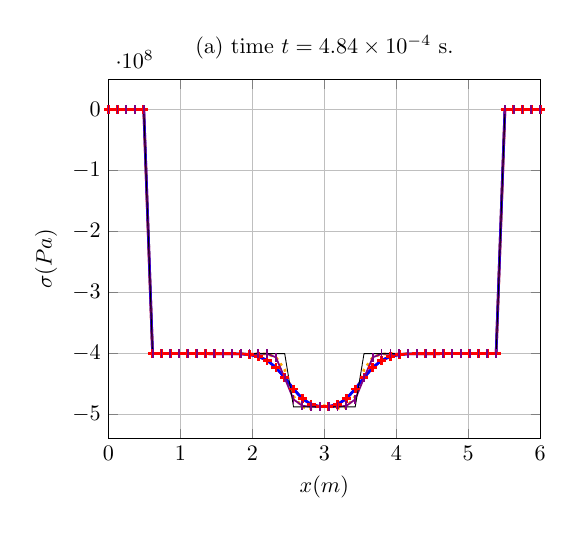
\begin{tikzpicture}[scale=0.8]
\begin{axis}[xlabel=$x (m)$,ylabel=$\sigma (Pa)$,ymajorgrids=true,xmajorgrids=true,legend pos=outer north east,title={(a) time $t = 4.84\times 10^{-4} $ s.},xmin=0.,xmax=6.]
\addplot[Red,very thick,mark=+,solid] coordinates {(0.0,-1.4032094709741823e-07) (0.12244897959183673,1.4032094709741797e-07) (0.24489795918367346,-5.501313561848306e-23) (0.36734693877551017,-1.4032094709741882e-07) (0.4897959183673469,-4.2096284129225576e-07) (0.6122448979591837,-400000000.0000052) (0.7346938775510203,-400000000.0003803) (0.8571428571428571,-400000000.0131417) (0.9795918367346939,-400000000.2874559) (1.1020408163265305,-400000004.46415013) (1.2244897959183674,-400000052.34678423) (1.346938775510204,-400000481.2046858) (1.4693877551020407,-400003554.03647596) (1.5918367346938775,-400021443.0967657) (1.7142857142857142,-400106894.9802318) (1.836734693877551,-400443646.6051052) (1.9591836734693877,-401540408.59283984) (2.0816326530612246,-404487333.2231472) (2.204081632653061,-410984305.87262785) (2.326530612244898,-422622254.02503896) (2.4489795918367347,-439299786.1010327) (2.571428571428571,-457971198.93456453) (2.693877551020408,-473710434.18348145) (2.816326530612245,-483108267.7934754) (2.9387755102040813,-486652315.1909913) (3.061224489795918,-486652315.1909913) (3.183673469387755,-483108267.7934754) (3.306122448979592,-473710434.18348145) (3.4285714285714284,-457971198.93456453) (3.5510204081632653,-439299786.1010328) (3.673469387755102,-422622254.025039) (3.7959183673469385,-410984305.8726279) (3.9183673469387754,-404487333.2231472) (4.040816326530612,-401540408.59283984) (4.163265306122449,-400443646.6051051) (4.285714285714286,-400106894.98023176) (4.408163265306122,-400021443.0967656) (4.530612244897959,-400003554.0364758) (4.653061224489796,-400000481.20468575) (4.775510204081632,-400000052.3467841) (4.8979591836734695,-400000004.46415013) (5.020408163265306,-400000000.2874559) (5.142857142857142,-400000000.01314175) (5.26530612244898,-400000000.0003803) (5.387755102040816,-400000000.0000052) (5.5102040816326525,1.403209470974181e-07) (5.63265306122449,-4.209628412922546e-07) (5.755102040816326,-7.335084749131074e-23) (5.877551020408163,-7.335084749131074e-23) (6.0,1.4032094709741816e-07) };
\addplot[Orange,very thick,mark=none,dotted] coordinates {(0.0011999999999999927,0.0) (0.12359999999999997,0.0) (0.24599999999999994,0.0) (0.36839999999999995,0.0) (0.4907999999999999,0.0) (0.6131999999999999,-399999999.9999996) (0.7355999999999999,-399999999.9999968) (0.858,-400000000.0) (0.9803999999999998,-399999999.9999996) (1.1027999999999998,-400000000.00000036) (1.2251999999999996,-400000000.0000013) (1.3475999999999997,-400000000.0000979) (1.4699999999999998,-400000000.00582314) (1.5923999999999996,-400000000.2649425) (1.7147999999999997,-400000009.2416795) (1.8371999999999995,-400000245.9026529) (1.9595999999999996,-400004932.9535555) (2.0819999999999994,-400073165.4563783) (2.2043999999999997,-400778734.27312934) (2.3267999999999995,-405684157.67745835) (2.4491999999999994,-426483554.2497189) (2.5715999999999997,-469882444.732417) (2.6939999999999995,-487460509.8573178) (2.8163999999999993,-489834934.6920107) (2.9387999999999996,-485390329.82597953) (3.0611999999999995,-485390329.8259847) (3.1835999999999993,-489834934.692009) (3.305999999999999,-487460509.85731673) (3.4283999999999994,-469882444.73241717) (3.5507999999999993,-426483554.2497191) (3.673199999999999,-405684157.67745817) (3.7955999999999994,-400778734.27312946) (3.9179999999999993,-400073165.4563784) (4.040399999999999,-400004932.95355564) (4.1628,-400000245.9026529) (4.2852,-400000009.2416795) (4.4076,-400000000.2649422) (4.53,-400000000.00582296) (4.6524,-400000000.0000977) (4.7748,-400000000.0000014) (4.8972,-400000000.00000036) (5.0196,-399999999.9999973) (5.142,-400000000.0) (5.2644,-400000000.0) (5.3868,-399999999.9999975) (5.5092,0.0) (5.6316,0.0) (5.754,0.0) (5.8764,0.0) (5.9988,0.0) };
\addplot[Blue,very thick,mark=none,solid] coordinates {(0.0011999999999999927,0.0) (0.12359999999999997,0.0) (0.24599999999999994,0.0) (0.36839999999999995,0.0) (0.4907999999999999,0.0) (0.6131999999999999,-400000000.0000052) (0.7355999999999999,-400000000.0003801) (0.858,-400000000.01314163) (0.9803999999999998,-400000000.2874559) (1.1027999999999998,-400000004.46415013) (1.2251999999999996,-400000052.3467841) (1.3475999999999997,-400000481.20468575) (1.4699999999999998,-400003554.03647584) (1.5923999999999996,-400021443.0967656) (1.7147999999999997,-400106894.9802317) (1.8371999999999995,-400443646.6051051) (1.9595999999999996,-401540408.5928399) (2.0819999999999994,-404487333.2231473) (2.2043999999999997,-410984305.8726279) (2.3267999999999995,-422622254.0250391) (2.4491999999999994,-439299786.10103285) (2.5715999999999997,-457971198.9345646) (2.6939999999999995,-473710434.1834816) (2.8163999999999993,-483108267.79347533) (2.9387999999999996,-486652315.1909914) (3.0611999999999995,-486652315.1909914) (3.1835999999999993,-483108267.79347533) (3.305999999999999,-473710434.1834816) (3.4283999999999994,-457971198.9345646) (3.5507999999999993,-439299786.10103285) (3.673199999999999,-422622254.0250391) (3.7955999999999994,-410984305.8726279) (3.9179999999999993,-404487333.2231473) (4.040399999999999,-401540408.5928399) (4.1628,-400443646.6051051) (4.2852,-400106894.9802317) (4.4076,-400021443.0967656) (4.53,-400003554.03647584) (4.6524,-400000481.20468575) (4.7748,-400000052.3467841) (4.8972,-400000004.46415013) (5.0196,-400000000.2874559) (5.142,-400000000.01314163) (5.2644,-400000000.0003801) (5.3868,-400000000.0000052) (5.5092,0.0) (5.6316,0.0) (5.754,0.0) (5.8764,0.0) (5.9988,0.0) };
\addplot[Purple,thick,mark=|,solid] coordinates {(0.0011999999999999927,0.0) (0.12359999999999997,0.0) (0.24599999999999994,0.0) (0.36839999999999995,0.0) (0.4907999999999999,0.0) (0.6131999999999999,-399999999.99999994) (0.7355999999999999,-400000000.0) (0.858,-400000000.0) (0.9803999999999998,-400000000.0) (1.1027999999999998,-400000000.0) (1.2251999999999996,-400000000.00000024) (1.3475999999999997,-400000000.00001407) (1.4699999999999998,-400000000.0007095) (1.5923999999999996,-400000000.0295273) (1.7147999999999997,-400000001.0283913) (1.8371999999999995,-400000030.33246076) (1.9595999999999996,-400000768.4378232) (2.0819999999999994,-400016975.1308303) (2.2043999999999997,-400318783.1149349) (2.3267999999999995,-405939608.94153374) (2.4491999999999994,-439871901.51192373) (2.5715999999999997,-475012040.0305417) (2.6939999999999995,-485411927.60231024) (2.8163999999999993,-487101987.7579666) (2.9387999999999996,-487278357.03341293) (3.0611999999999995,-487278357.03341293) (3.1835999999999993,-487101987.7579666) (3.305999999999999,-485411927.60231024) (3.4283999999999994,-475012040.0305417) (3.5507999999999993,-439871901.51192373) (3.673199999999999,-405939608.94153374) (3.7955999999999994,-400318783.1149349) (3.9179999999999993,-400016975.1308303) (4.040399999999999,-400000768.4378232) (4.1628,-400000030.33246076) (4.2852,-400000001.0283913) (4.4076,-400000000.0295273) (4.53,-400000000.0007095) (4.6524,-400000000.00001407) (4.7748,-400000000.0000003) (4.8972,-400000000.0) (5.0196,-400000000.0) (5.142,-400000000.0) (5.2644,-400000000.0) (5.3868,-399999999.99999994) (5.5092,0.0) (5.6316,0.0) (5.754,0.0) (5.8764,0.0) (5.9988,0.0) };
\addplot[black,thin,mark=none,solid] coordinates {(0.0,-0.0) (0.12244897959183673,-0.0) (0.24489795918367346,-0.0) (0.36734693877551017,-0.0) (0.4897959183673469,-0.0) (0.6122448979591837,-400000000.0) (0.7346938775510203,-400000000.0) (0.8571428571428571,-400000000.0) (0.9795918367346939,-400000000.0) (1.1020408163265305,-400000000.0) (1.2244897959183674,-400000000.0) (1.346938775510204,-400000000.0) (1.4693877551020407,-400000000.0) (1.5918367346938775,-400000000.0) (1.7142857142857142,-400000000.0) (1.836734693877551,-400000000.0) (1.9591836734693877,-400000000.0) (2.0816326530612246,-400000000.0) (2.204081632653061,-400000000.0) (2.326530612244898,-400000000.0) (2.4489795918367347,-400000000.0) (2.571428571428571,-487287156.09439695) (2.693877551020408,-487287156.09439695) (2.816326530612245,-487287156.09439695) (2.9387755102040813,-487287156.09439695) (3.061224489795918,-487287156.09439695) (3.183673469387755,-487287156.09439695) (3.306122448979592,-487287156.09439695) (3.4285714285714284,-487287156.09439695) (3.5510204081632653,-400000000.0) (3.673469387755102,-400000000.0) (3.7959183673469385,-400000000.0) (3.9183673469387754,-400000000.0) (4.040816326530612,-400000000.0) (4.163265306122449,-400000000.0) (4.285714285714286,-400000000.0) (4.408163265306122,-400000000.0) (4.530612244897959,-400000000.0) (4.653061224489796,-400000000.0) (4.775510204081632,-400000000.0) (4.8979591836734695,-400000000.0) (5.020408163265306,-400000000.0) (5.142857142857142,-400000000.0) (5.26530612244898,-400000000.0) (5.387755102040816,-400000000.0) (5.5102040816326525,-0.0) (5.63265306122449,-0.0) (5.755102040816326,-0.0) (5.877551020408163,-0.0) (6.0,-0.0) };
%\legend{dgmpm,fem,fvm,fvm (SB),exact}
\end{axis}
\end{tikzpicture}
%%% Local Variables:
%%% mode: latex
%%% TeX-master: "../../mainManuscript"
%%% End:
}
  {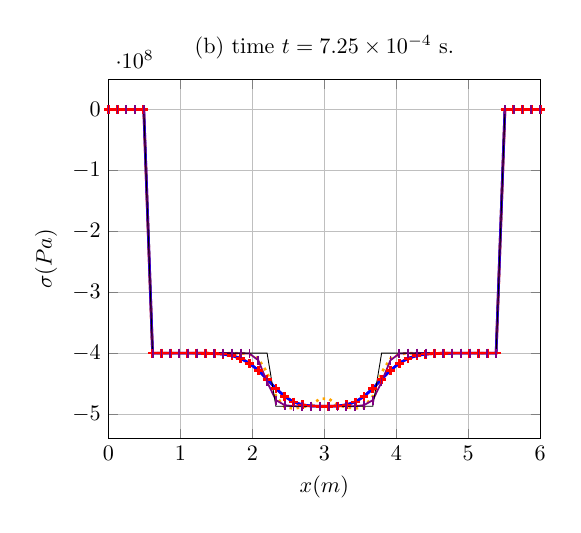
\begin{tikzpicture}[scale=0.8]
\begin{axis}[xlabel=$x (m)$,ylabel=$\sigma (Pa)$,ymajorgrids=true,xmajorgrids=true,legend pos=outer north east,title={(b) time $t = 7.25\times 10^{-4} $ s.},xmin=0.,xmax=6.]
\addplot[Red,very thick,mark=+,solid] coordinates {(0.0,-0.016398596440346053) (0.12244897959183673,-0.06425322857955201) (0.24489795918367346,-0.7380674881804443) (0.36734693877551017,-2.12047390173559) (0.4897959183673469,-28.76271861558054) (0.6122448979591837,-400000015.4159754) (0.7346938775510203,-400000102.7573024) (0.8571428571428571,-400000598.1932516) (0.9795918367346939,-400003055.79803795) (1.1020408163265305,-400013747.0436081) (1.2244897959183674,-400054602.7199052) (1.346938775510204,-400191823.2382515) (1.4693877551020407,-400596672.6802674) (1.5918367346938775,-401644186.51493835) (1.7142857142857142,-404014374.4754996) (1.836734693877551,-408684632.25449073) (1.9591836734693877,-416652037.9726774) (2.0816326530612246,-428329061.0045163) (2.204081632653061,-442879954.5361007) (2.326530612244898,-458084443.80872595) (2.4489795918367347,-471157539.9020842) (2.571428571428571,-480164339.19475454) (2.693877551020408,-484944715.5259052) (2.816326530612245,-486779650.5319825) (2.9387755102040813,-487233015.60471344) (3.061224489795918,-487233015.60471344) (3.183673469387755,-486779650.5319825) (3.306122448979592,-484944715.5259052) (3.4285714285714284,-480164339.19475454) (3.5510204081632653,-471157539.9020842) (3.673469387755102,-458084443.80872613) (3.7959183673469385,-442879954.5361007) (3.9183673469387754,-428329061.0045163) (4.040816326530612,-416652037.9726776) (4.163265306122449,-408684632.2544908) (4.285714285714286,-404014374.4754996) (4.408163265306122,-401644186.5149382) (4.530612244897959,-400596672.68026733) (4.653061224489796,-400191823.2382513) (4.775510204081632,-400054602.7199051) (4.8979591836734695,-400013747.04360807) (5.020408163265306,-400003055.79803795) (5.142857142857142,-400000598.19325155) (5.26530612244898,-400000102.75730234) (5.387755102040816,-400000015.4159754) (5.5102040816326525,-28.762718512303003) (5.63265306122449,-2.1204742438100417) (5.755102040816326,-0.7380675867576459) (5.877551020408163,-0.06425320166977637) (6.0,-0.01639854380134023) };
\addplot[Orange,very thick,mark=none,dotted] coordinates {(0.0011999999999999927,0.0) (0.12359999999999997,2.8345154836222343e-06) (0.24599999999999994,0.0) (0.36839999999999995,-5.6690309672444694e-06) (0.4907999999999999,5.563100179036459e-06) (0.6131999999999999,-400000000.00000036) (0.7355999999999999,-400000000.00000095) (0.858,-400000000.0000158) (0.9803999999999998,-400000000.000588) (1.1027999999999998,-400000000.0183558) (1.2251999999999996,-400000000.47669524) (1.3475999999999997,-400000010.242256) (1.4699999999999998,-400000180.58382314) (1.5923999999999996,-400002583.79875094) (1.7147999999999997,-400029558.11391515) (1.8371999999999995,-400265019.7421873) (1.9595999999999996,-401812442.4208182) (2.0819999999999994,-409100274.22059995) (2.2043999999999997,-431724216.84982246) (2.3267999999999995,-470516941.3021229) (2.4491999999999994,-488918339.55243546) (2.5715999999999997,-490903509.0666595) (2.6939999999999995,-488910392.160918) (2.8163999999999993,-485129466.2005724) (2.9387999999999996,-474875832.26573056) (3.0611999999999995,-474875832.26572955) (3.1835999999999993,-485129466.20057756) (3.305999999999999,-488910392.1609156) (3.4283999999999994,-490903509.0666595) (3.5507999999999993,-488918339.5524351) (3.673199999999999,-470516941.30212307) (3.7955999999999994,-431724216.8498228) (3.9179999999999993,-409100274.22060007) (4.040399999999999,-401812442.42081815) (4.1628,-400265019.742187) (4.2852,-400029558.11391526) (4.4076,-400002583.79875064) (4.53,-400000180.5838233) (4.6524,-400000010.242256) (4.7748,-400000000.47669554) (4.8972,-400000000.01835567) (5.0196,-400000000.00058854) (5.142,-400000000.00001574) (5.2644,-400000000.0000007) (5.3868,-400000000.0) (5.5092,-2.660415564296186e-06) (5.6316,-2.493917513477148e-06) (5.754,-2.7171818926536604e-06) (5.8764,3.405979701450893e-07) (5.9988,-2.8345154836222373e-06) };
\addplot[Blue,very thick,mark=none,solid] coordinates {(0.0011999999999999927,-0.00357849008468239) (0.12359999999999997,-0.06440079814818947) (0.24599999999999994,-0.21143910174666652) (0.36839999999999995,-2.1204748738318564) (0.4907999999999999,-3.2714037895202637) (0.6131999999999999,-400000015.4159753) (0.7355999999999999,-400000102.75730234) (0.858,-400000598.1932516) (0.9803999999999998,-400003055.79803795) (1.1027999999999998,-400013747.04360807) (1.2251999999999996,-400054602.7199051) (1.3475999999999997,-400191823.2382513) (1.4699999999999998,-400596672.68026733) (1.5923999999999996,-401644186.5149383) (1.7147999999999997,-404014374.47549963) (1.8371999999999995,-408684632.25449085) (1.9595999999999996,-416652037.9726776) (2.0819999999999994,-428329061.00451636) (2.2043999999999997,-442879954.5361008) (2.3267999999999995,-458084443.80872625) (2.4491999999999994,-471157539.9020842) (2.5715999999999997,-480164339.1947546) (2.6939999999999995,-484944715.52590525) (2.8163999999999993,-486779650.5319826) (2.9387999999999996,-487233015.60471344) (3.0611999999999995,-487233015.60471344) (3.1835999999999993,-486779650.5319826) (3.305999999999999,-484944715.52590525) (3.4283999999999994,-480164339.1947546) (3.5507999999999993,-471157539.9020842) (3.673199999999999,-458084443.80872625) (3.7955999999999994,-442879954.5361008) (3.9179999999999993,-428329061.00451636) (4.040399999999999,-416652037.9726776) (4.1628,-408684632.25449085) (4.2852,-404014374.47549963) (4.4076,-401644186.5149383) (4.53,-400596672.68026733) (4.6524,-400191823.2382513) (4.7748,-400054602.7199051) (4.8972,-400013747.04360807) (5.0196,-400003055.79803795) (5.142,-400000598.1932516) (5.2644,-400000102.75730234) (5.3868,-400000015.4159753) (5.5092,-3.2714037895202637) (5.6316,-2.1204748738318564) (5.754,-0.21143910174666652) (5.8764,-0.06440079814818947) (5.9988,-0.00357849008468239) };
\addplot[Purple,thick,mark=|,solid] coordinates {(0.0011999999999999927,1.6543612251060583e-24) (0.12359999999999997,1.6543612251060553e-23) (0.24599999999999994,2.452440800103604e-08) (0.36839999999999995,-3.508023677435457e-08) (0.4907999999999999,-5.960464477539063e-08) (0.6131999999999999,-400000000.0) (0.7355999999999999,-400000000.0) (0.858,-400000000.0000003) (0.9803999999999998,-400000000.0000133) (1.1027999999999998,-400000000.0004144) (1.2251999999999996,-400000000.0115142) (1.3475999999999997,-400000000.2871339) (1.4699999999999998,-400000006.46675307) (1.5923999999999996,-400000132.73197645) (1.7147999999999997,-400002510.7191475) (1.8371999999999995,-400043970.06492174) (1.9595999999999996,-400741455.361692) (2.0819999999999994,-411776022.67189264) (2.2043999999999997,-447347518.96724993) (2.3267999999999995,-477210124.05958325) (2.4491999999999994,-485453941.80645174) (2.5715999999999997,-487021615.6680456) (2.6939999999999995,-487258956.9032909) (2.8163999999999993,-487285223.6098061) (2.9387999999999996,-487287092.0986835) (3.0611999999999995,-487287092.0986835) (3.1835999999999993,-487285223.6098061) (3.305999999999999,-487258956.9032909) (3.4283999999999994,-487021615.6680456) (3.5507999999999993,-485453941.80645174) (3.673199999999999,-477210124.05958325) (3.7955999999999994,-447347518.96724993) (3.9179999999999993,-411776022.67189264) (4.040399999999999,-400741455.361692) (4.1628,-400043970.06492174) (4.2852,-400002510.71914756) (4.4076,-400000132.73197645) (4.53,-400000006.466753) (4.6524,-400000000.287134) (4.7748,-400000000.01151425) (4.8972,-400000000.0004144) (5.0196,-400000000.0000133) (5.142,-400000000.0000003) (5.2644,-400000000.0) (5.3868,-400000000.0) (5.5092,-5.960464477539063e-08) (5.6316,-3.508023677435457e-08) (5.754,2.452440800103604e-08) (5.8764,1.6543612251060553e-23) (5.9988,1.6543612251060583e-24) };
\addplot[black,thin,mark=none,solid] coordinates {(0.0,-0.0) (0.12244897959183673,-0.0) (0.24489795918367346,-0.0) (0.36734693877551017,-0.0) (0.4897959183673469,-0.0) (0.6122448979591837,-400000000.0) (0.7346938775510203,-400000000.0) (0.8571428571428571,-400000000.0) (0.9795918367346939,-400000000.0) (1.1020408163265305,-400000000.0) (1.2244897959183674,-400000000.0) (1.346938775510204,-400000000.0) (1.4693877551020407,-400000000.0) (1.5918367346938775,-400000000.0) (1.7142857142857142,-400000000.0) (1.836734693877551,-400000000.0) (1.9591836734693877,-400000000.0) (2.0816326530612246,-400000000.0) (2.204081632653061,-400000000.0) (2.326530612244898,-487287156.09439695) (2.4489795918367347,-487287156.09439695) (2.571428571428571,-487287156.09439695) (2.693877551020408,-487287156.09439695) (2.816326530612245,-487287156.09439695) (2.9387755102040813,-487287156.09439695) (3.061224489795918,-487287156.09439695) (3.183673469387755,-487287156.09439695) (3.306122448979592,-487287156.09439695) (3.4285714285714284,-487287156.09439695) (3.5510204081632653,-487287156.09439695) (3.673469387755102,-487287156.09439695) (3.7959183673469385,-400000000.0) (3.9183673469387754,-400000000.0) (4.040816326530612,-400000000.0) (4.163265306122449,-400000000.0) (4.285714285714286,-400000000.0) (4.408163265306122,-400000000.0) (4.530612244897959,-400000000.0) (4.653061224489796,-400000000.0) (4.775510204081632,-400000000.0) (4.8979591836734695,-400000000.0) (5.020408163265306,-400000000.0) (5.142857142857142,-400000000.0) (5.26530612244898,-400000000.0) (5.387755102040816,-400000000.0) (5.5102040816326525,-0.0) (5.63265306122449,-0.0) (5.755102040816326,-0.0) (5.877551020408163,-0.0) (6.0,-0.0) };
%\legend{dgmpm,fem,fvm,fvm (SB),exact}
\end{axis}
\end{tikzpicture}
%%% Local Variables:
%%% mode: latex
%%% TeX-master: "../../mainManuscript"
%%% End:
}
  {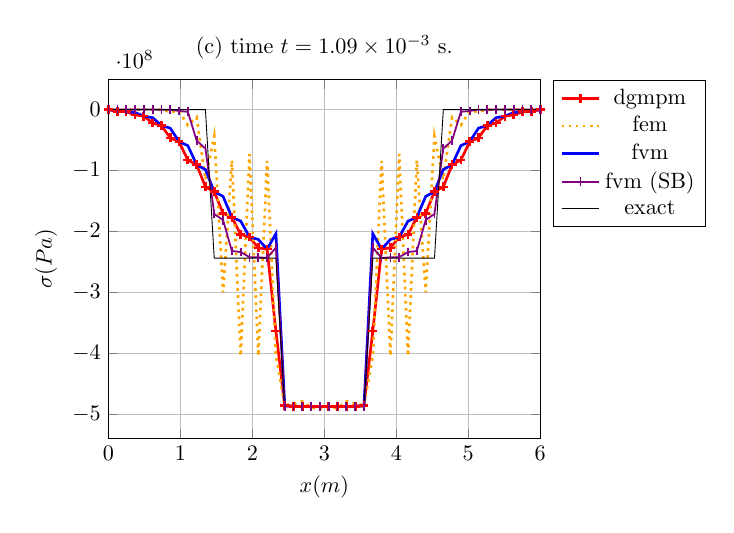
\begin{tikzpicture}[scale=0.8]
\begin{axis}[xlabel=$x (m)$,ylabel=$\sigma (Pa)$,ymajorgrids=true,xmajorgrids=true,legend pos=outer north east,title={(c) time $t = 1.09\times 10^{-3} $ s.},xmin=0.,xmax=6.]
\addplot[Red,very thick,mark=+,solid] coordinates {(0.0,-298852.1952411225) (0.12244897959183673,-2592980.4740912793) (0.24489795918367346,-3560236.4322381816) (0.36734693877551017,-8652722.221047912) (0.4897959183673469,-10777216.673686886) (0.6122448979591837,-21974314.707157355) (0.7346938775510203,-26009924.918005344) (0.8571428571428571,-46347563.10657899) (0.9795918367346939,-52593345.171819046) (1.1020408163265305,-82683979.65035231) (1.2244897959183674,-90525380.97285904) (1.346938775510204,-126773557.44849168) (1.4693877551020407,-134743667.28836828) (1.5918367346938775,-170219249.4978279) (1.7142857142857142,-176744937.7749974) (1.836734693877551,-204799464.24688196) (1.9591836734693877,-209064122.25232974) (2.0816326530612246,-226820170.49378502) (2.204081632653061,-229011964.3130221) (2.326530612244898,-363270795.9137317) (2.4489795918367347,-485529213.90073514) (2.571428571428571,-486748760.1951447) (2.693877551020408,-487164866.56783277) (2.816326530612245,-487268871.16624963) (2.9387755102040813,-487285807.7274521) (3.061224489795918,-487285807.7274521) (3.183673469387755,-487268871.16624963) (3.306122448979592,-487164866.56783277) (3.4285714285714284,-486748760.1951447) (3.5510204081632653,-485529213.90073514) (3.673469387755102,-363270795.91372997) (3.7959183673469385,-229011964.3130223) (3.9183673469387754,-226820170.49378502) (4.040816326530612,-209064122.25232938) (4.163265306122449,-204799464.2468816) (4.285714285714286,-176744937.77499697) (4.408163265306122,-170219249.4978276) (4.530612244897959,-134743667.28836808) (4.653061224489796,-126773557.44849148) (4.775510204081632,-90525380.9728589) (4.8979591836734695,-82683979.65035222) (5.020408163265306,-52593345.171819076) (5.142857142857142,-46347563.10657902) (5.26530612244898,-26009924.918005634) (5.387755102040816,-21974314.707157686) (5.5102040816326525,-10777216.673687106) (5.63265306122449,-8652722.22104813) (5.755102040816326,-3560236.4322383474) (5.877551020408163,-2592980.4740913147) (6.0,-298852.1952412414) };
\addplot[Orange,very thick,mark=none,dotted] coordinates {(0.0011999999999999927,-8.564176737061382) (0.12359999999999997,-888.6628072166062) (0.24599999999999994,-978.957275855234) (0.36839999999999995,-20655.627263077142) (0.4907999999999999,-18896.641533666516) (0.6131999999999999,-330216.80702995) (0.7355999999999999,-249388.69343146865) (0.858,-3578975.198424924) (0.9803999999999998,-2204497.3282262576) (1.1027999999999998,-25572627.543806504) (1.2251999999999996,-12586085.323168479) (1.3475999999999997,-114927967.2865971) (1.4699999999999998,-43662060.649838395) (1.5923999999999996,-299930609.4383477) (1.7147999999999997,-83159988.2807549) (1.8371999999999995,-404308497.6800079) (1.9595999999999996,-73354055.19993815) (2.0819999999999994,-404115446.2975375) (2.2043999999999997,-84185546.45762134) (2.3267999999999995,-404377932.87605923) (2.4491999999999994,-484698403.52376723) (2.5715999999999997,-483271039.38939494) (2.6939999999999995,-478503258.5469886) (2.8163999999999993,-489364428.59318465) (2.9387999999999996,-490415003.4350529) (3.0611999999999995,-490415003.4350446) (3.1835999999999993,-489364428.59318817) (3.305999999999999,-478503258.54699033) (3.4283999999999994,-483271039.3893873) (3.5507999999999993,-484698403.5237801) (3.673199999999999,-404377932.8760693) (3.7955999999999994,-84185546.45760433) (3.9179999999999993,-404115446.2975594) (4.040399999999999,-73354055.19990571) (4.1628,-404308497.68004787) (4.2852,-83159988.28071125) (4.4076,-299930609.4383874) (4.53,-43662060.64979588) (4.6524,-114927967.28663965) (4.7748,-12586085.323131083) (4.8972,-25572627.5438284) (5.0196,-2204497.328220724) (5.142,-3578975.198433095) (5.2644,-249388.6934192833) (5.3868,-330216.80704583385) (5.5092,-18896.641507875855) (5.6316,-20655.627279743658) (5.754,-978.9572757378946) (5.8764,-888.6628068760092) (5.9988,-8.564168233514941) };
\addplot[Blue,very thick,mark=none,solid] coordinates {(0.0011999999999999927,-697321.7888962623) (0.12359999999999997,-1197941.6218375992) (0.24599999999999994,-3649678.3886538874) (0.36839999999999995,-4760949.893544708) (0.4907999999999999,-10792700.069992812) (0.6131999999999999,-13236107.179622345) (0.7355999999999999,-26011940.413994417) (0.858,-30449976.911887925) (0.9803999999999998,-52593535.76622025) (1.1027999999999998,-59159850.537988245) (1.2251999999999996,-90525393.4487186) (1.3475999999999997,-98435394.04413308) (1.4699999999999998,-134743667.81499696) (1.5923999999999996,-142485074.51963878) (1.7147999999999997,-176744937.78781757) (1.8371999999999995,-182866937.3660821) (1.9595999999999996,-209064122.25247735) (2.0819999999999994,-212938809.63865638) (2.2043999999999997,-229011964.31302345) (2.3267999999999995,-203580656.03460932) (2.4491999999999994,-485529213.90073514) (2.5715999999999997,-486748760.19514465) (2.6939999999999995,-487164866.56783277) (2.8163999999999993,-487268871.16624963) (2.9387999999999996,-487285807.72745204) (3.0611999999999995,-487285807.72745204) (3.1835999999999993,-487268871.16624963) (3.305999999999999,-487164866.56783277) (3.4283999999999994,-486748760.19514465) (3.5507999999999993,-485529213.90073514) (3.673199999999999,-203580656.03460932) (3.7955999999999994,-229011964.31302345) (3.9179999999999993,-212938809.63865638) (4.040399999999999,-209064122.25247735) (4.1628,-182866937.3660821) (4.2852,-176744937.78781757) (4.4076,-142485074.51963878) (4.53,-134743667.81499696) (4.6524,-98435394.04413308) (4.7748,-90525393.4487186) (4.8972,-59159850.537988245) (5.0196,-52593535.76622025) (5.142,-30449976.911887925) (5.2644,-26011940.413994417) (5.3868,-13236107.179622345) (5.5092,-10792700.069992812) (5.6316,-4760949.893544708) (5.754,-3649678.3886538874) (5.8764,-1197941.6218375992) (5.9988,-697321.7888962623) };
\addplot[Purple,thick,mark=|,solid] coordinates {(0.0011999999999999927,-1.5776833891868591) (0.12359999999999997,-3.1103133444301605) (0.24599999999999994,-66.3245544020645) (0.36839999999999995,-120.53058021211032) (0.4907999999999999,-2323.981773991816) (0.6131999999999999,-4077.7229402686107) (0.7355999999999999,-73476.02839571485) (0.858,-125223.90384372801) (0.9803999999999998,-2192061.988010791) (1.1027999999999998,-3654289.9822202735) (1.2251999999999996,-50836136.514345884) (1.3475999999999997,-64090238.476814374) (1.4699999999999998,-171321971.71407443) (1.5923999999999996,-181320649.43958035) (1.7147999999999997,-232008895.73718417) (1.8371999999999995,-233742433.76137352) (1.9595999999999996,-242083509.85309348) (2.0819999999999994,-242332334.00719002) (2.2043999999999997,-243472921.17509142) (2.3267999999999995,-226316133.38373914) (2.4491999999999994,-487281912.7980076) (2.5715999999999997,-487286639.11155045) (2.6939999999999995,-487287118.8214492) (2.8163999999999993,-487287154.35078365) (2.9387999999999996,-487287156.054703) (3.0611999999999995,-487287156.054703) (3.1835999999999993,-487287154.35078365) (3.305999999999999,-487287118.8214492) (3.4283999999999994,-487286639.11155045) (3.5507999999999993,-487281912.7980076) (3.673199999999999,-226316133.38373917) (3.7955999999999994,-243472921.17509145) (3.9179999999999993,-242332334.00719002) (4.040399999999999,-242083509.85309348) (4.1628,-233742433.7613735) (4.2852,-232008895.73718417) (4.4076,-181320649.4395804) (4.53,-171321971.7140746) (4.6524,-64090238.47681402) (4.7748,-50836136.51434556) (4.8972,-3654289.982220319) (5.0196,-2192061.9880108386) (5.142,-125223.90384437214) (5.2644,-73476.02839642452) (5.3868,-4077.7229395179684) (5.5092,-2323.9817731909106) (5.6316,-120.53058021586685) (5.754,-66.32455442257307) (5.8764,-3.1103136033573158) (5.9988,-1.5776836574077606) };
\addplot[black,thin,mark=none,solid] coordinates {(0.0,-0.0) (0.12244897959183673,-0.0) (0.24489795918367346,-0.0) (0.36734693877551017,-0.0) (0.4897959183673469,-0.0) (0.6122448979591837,-0.0) (0.7346938775510203,-0.0) (0.8571428571428571,-0.0) (0.9795918367346939,-0.0) (1.1020408163265305,-0.0) (1.2244897959183674,-0.0) (1.346938775510204,-0.0) (1.4693877551020407,-243643578.04719847) (1.5918367346938775,-243643578.04719847) (1.7142857142857142,-243643578.04719847) (1.836734693877551,-243643578.04719847) (1.9591836734693877,-243643578.04719847) (2.0816326530612246,-243643578.04719847) (2.204081632653061,-243643578.04719847) (2.326530612244898,-243643578.04719847) (2.4489795918367347,-487287156.09439695) (2.571428571428571,-487287156.09439695) (2.693877551020408,-487287156.09439695) (2.816326530612245,-487287156.09439695) (2.9387755102040813,-487287156.09439695) (3.061224489795918,-487287156.09439695) (3.183673469387755,-487287156.09439695) (3.306122448979592,-487287156.09439695) (3.4285714285714284,-487287156.09439695) (3.5510204081632653,-487287156.09439695) (3.673469387755102,-243643578.04719847) (3.7959183673469385,-243643578.04719847) (3.9183673469387754,-243643578.04719847) (4.040816326530612,-243643578.04719847) (4.163265306122449,-243643578.04719847) (4.285714285714286,-243643578.04719847) (4.408163265306122,-243643578.04719847) (4.530612244897959,-243643578.04719847) (4.653061224489796,-0.0) (4.775510204081632,-0.0) (4.8979591836734695,-0.0) (5.020408163265306,-0.0) (5.142857142857142,-0.0) (5.26530612244898,-0.0) (5.387755102040816,-0.0) (5.5102040816326525,-0.0) (5.63265306122449,-0.0) (5.755102040816326,-0.0) (5.877551020408163,-0.0) (6.0,-0.0) };
\legend{dgmpm,fem,fvm,fvm (SB),exact}
\end{axis}
\end{tikzpicture}
%%% Local Variables:
%%% mode: latex
%%% TeX-master: "../../mainManuscript"
%%% End:
}
  \caption{elastic-plastic RP stress}
  \label{fig:stress_elastoplastic_RP}
\end{figure}
\begin{figure}[h!]
  \centering
  {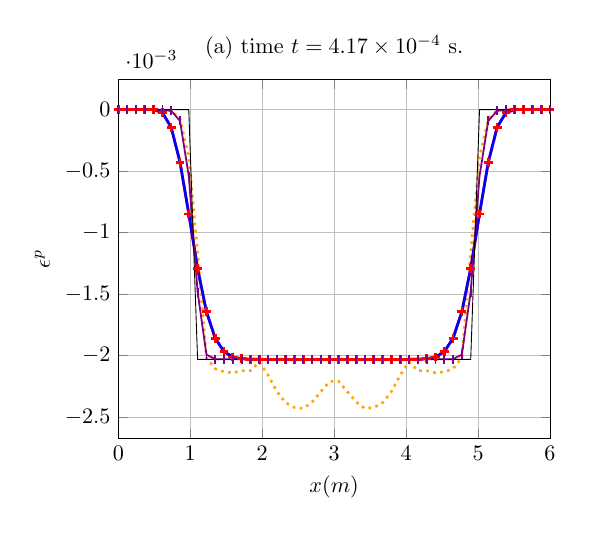
\begin{tikzpicture}[scale=0.8]
\begin{axis}[xlabel=$x (m)$,ylabel=$\epsilon^p$,ymajorgrids=true,xmajorgrids=true,legend pos=outer north east,title={(a) time $t = 4.17\times 10^{-4} $ s.},xmin=0.,xmax=6.]
\addplot[Red,very thick,mark=+,solid] coordinates {(0.0,0.0) (0.12244897959183673,0.0) (0.24489795918367346,0.0) (0.36734693877551017,0.0) (0.4897959183673469,0.0) (0.6122448979591837,-2.4267855226065594e-05) (0.7346938775510203,-0.00014452073597361284) (0.8571428571428571,-0.0004275642401009131) (0.9795918367346939,-0.0008483282066457896) (1.1020408163265305,-0.0012913872123487611) (1.2244897959183674,-0.001642660920094959) (1.346938775510204,-0.0018602413103573651) (1.4693877551020407,-0.0019680574666657586) (1.5918367346938775,-0.00201146561977191) (1.7142857142857142,-0.002025805454394895) (1.836734693877551,-0.0020297136017104972) (1.9591836734693877,-0.002030593864489664) (2.0816326530612246,-0.002030757436013639) (2.204081632653061,-0.0020307823755532774) (2.326530612244898,-0.002030785465084119) (2.4489795918367347,-0.0020307857712710334) (2.571428571428571,-0.00203078579497771) (2.693877551020408,-0.0020307857963597366) (2.816326530612245,-0.002030785796416807) (2.9387755102040813,-0.002030785796418294) (3.061224489795918,-0.002030785796418294) (3.183673469387755,-0.0020307857964168056) (3.306122448979592,-0.002030785796359739) (3.4285714285714284,-0.0020307857949777124) (3.5510204081632653,-0.002030785771271032) (3.673469387755102,-0.002030785465084119) (3.7959183673469385,-0.002030782375553277) (3.9183673469387754,-0.0020307574360136386) (4.040816326530612,-0.002030593864489664) (4.163265306122449,-0.0020297136017104964) (4.285714285714286,-0.0020258054543948927) (4.408163265306122,-0.002011465619771909) (4.530612244897959,-0.0019680574666657573) (4.653061224489796,-0.0018602413103573651) (4.775510204081632,-0.0016426609200949592) (4.8979591836734695,-0.001291387212348762) (5.020408163265306,-0.0008483282066457893) (5.142857142857142,-0.00042756424010091193) (5.26530612244898,-0.00014452073597361384) (5.387755102040816,-2.4267855226067292e-05) (5.5102040816326525,0.0) (5.63265306122449,0.0) (5.755102040816326,0.0) (5.877551020408163,0.0) (6.0,0.0) };
\addplot[Orange,very thick,mark=none,dotted] coordinates {(0.0011999999999999927,0.0) (0.12359999999999997,0.0) (0.24599999999999994,0.0) (0.36839999999999995,0.0) (0.4907999999999999,0.0) (0.6131999999999999,-3.6185144371068533e-07) (0.7355999999999999,-8.019549939201378e-06) (0.858,-7.545863055389513e-05) (0.9803999999999998,-0.00038823448768833166) (1.1027999999999998,-0.0011649510446652884) (1.2251999999999996,-0.0020167797859788647) (1.3475999999999997,-0.002107399619958115) (1.4699999999999998,-0.002131770374563102) (1.5923999999999996,-0.0021403574192086572) (1.7147999999999997,-0.0021224712498380525) (1.8371999999999995,-0.0021223153729543927) (1.9595999999999996,-0.002051517588290279) (2.0819999999999994,-0.00215869886386764) (2.2043999999999997,-0.00229323761080671) (2.3267999999999995,-0.002383730340592019) (2.4491999999999994,-0.002422023782426279) (2.5715999999999997,-0.0024301527006305407) (2.6939999999999995,-0.0023776240406298606) (2.8163999999999993,-0.0022924966391795762) (2.9387999999999996,-0.002209718054457858) (3.0611999999999995,-0.002209718054457853) (3.1835999999999993,-0.00229249663917957) (3.305999999999999,-0.002377624040629834) (3.4283999999999994,-0.0024301527006305133) (3.5507999999999993,-0.0024220237824262893) (3.673199999999999,-0.0023837303405920274) (3.7955999999999994,-0.0022932376108067225) (3.9179999999999993,-0.002158698863867652) (4.040399999999999,-0.0020515175882902612) (4.1628,-0.00212231537295439) (4.2852,-0.002122471249838043) (4.4076,-0.002140357419208655) (4.53,-0.0021317703745630944) (4.6524,-0.0021073996199581038) (4.7748,-0.002016779785978835) (4.8972,-0.0011649510446653149) (5.0196,-0.00038823448768831226) (5.142,-7.54586305539126e-05) (5.2644,-8.019549939178096e-06) (5.3868,-3.6185144371335306e-07) (5.5092,0.0) (5.6316,0.0) (5.754,0.0) (5.8764,0.0) (5.9988,0.0) };
\addplot[Blue,very thick,mark=none,solid] coordinates {(0.0011999999999999927,0.0) (0.12359999999999997,0.0) (0.24599999999999994,0.0) (0.36839999999999995,0.0) (0.4907999999999999,0.0) (0.6131999999999999,-2.4267855226066533e-05) (0.7355999999999999,-0.00014452073597361162) (0.858,-0.0004275642401009113) (0.9803999999999998,-0.0008483282066457879) (1.1027999999999998,-0.0012913872123487594) (1.2251999999999996,-0.0016426609200949575) (1.3475999999999997,-0.0018602413103573636) (1.4699999999999998,-0.0019680574666657573) (1.5923999999999996,-0.002011465619771908) (1.7147999999999997,-0.002025805454394894) (1.8371999999999995,-0.0020297136017104955) (1.9595999999999996,-0.0020305938644896646) (2.0819999999999994,-0.002030757436013637) (2.2043999999999997,-0.002030782375553278) (2.3267999999999995,-0.002030785465084118) (2.4491999999999994,-0.0020307857712710316) (2.5715999999999997,-0.002030785794977712) (2.6939999999999995,-0.002030785796359737) (2.8163999999999993,-0.002030785796416805) (2.9387999999999996,-0.0020307857964182922) (3.0611999999999995,-0.0020307857964182935) (3.1835999999999993,-0.002030785796416805) (3.305999999999999,-0.002030785796359737) (3.4283999999999994,-0.002030785794977712) (3.5507999999999993,-0.0020307857712710316) (3.673199999999999,-0.0020307854650841186) (3.7955999999999994,-0.002030782375553278) (3.9179999999999993,-0.002030757436013637) (4.040399999999999,-0.0020305938644896646) (4.1628,-0.0020297136017104955) (4.2852,-0.002025805454394893) (4.4076,-0.002011465619771907) (4.53,-0.0019680574666657573) (4.6524,-0.0018602413103573636) (4.7748,-0.0016426609200949566) (4.8972,-0.0012913872123487594) (5.0196,-0.0008483282066457876) (5.142,-0.0004275642401009109) (5.2644,-0.00014452073597361162) (5.3868,-2.4267855226066533e-05) (5.5092,0.0) (5.6316,0.0) (5.754,0.0) (5.8764,0.0) (5.9988,0.0) };
\addplot[Purple,thick,mark=|,solid] coordinates {(0.0011999999999999927,0.0) (0.12359999999999997,0.0) (0.24599999999999994,0.0) (0.36839999999999995,0.0) (0.4907999999999999,0.0) (0.6131999999999999,-5.394021759754931e-07) (0.7355999999999999,-1.010771354391672e-05) (0.858,-9.168096769918878e-05) (0.9803999999999998,-0.0005435535234499527) (1.1027999999999998,-0.0014841083655069223) (1.2251999999999996,-0.001991887176242578) (1.3475999999999997,-0.002028854598935097) (1.4699999999999998,-0.0020307027185062754) (1.5923999999999996,-0.002030782602337539) (1.7147999999999997,-0.0020307856903745234) (1.8371999999999995,-0.002030785793411752) (1.9595999999999996,-0.002030785796346042) (2.0819999999999994,-0.002030785796416862) (2.2043999999999997,-0.002030785796418289) (2.3267999999999995,-0.0020307857964183135) (2.4491999999999994,-0.0020307857964183135) (2.5715999999999997,-0.0020307857964183135) (2.6939999999999995,-0.0020307857964183135) (2.8163999999999993,-0.0020307857964183135) (2.9387999999999996,-0.0020307857964183135) (3.0611999999999995,-0.0020307857964183135) (3.1835999999999993,-0.0020307857964183135) (3.305999999999999,-0.0020307857964183126) (3.4283999999999994,-0.0020307857964183135) (3.5507999999999993,-0.0020307857964183126) (3.673199999999999,-0.0020307857964183126) (3.7955999999999994,-0.002030785796418291) (3.9179999999999993,-0.0020307857964168632) (4.040399999999999,-0.0020307857963460427) (4.1628,-0.0020307857934117523) (4.2852,-0.002030785690374525) (4.4076,-0.0020307826023375384) (4.53,-0.0020307027185062733) (4.6524,-0.002028854598935106) (4.7748,-0.0019918871762425686) (4.8972,-0.0014841083655069208) (5.0196,-0.0005435535234499549) (5.142,-9.168096769918878e-05) (5.2644,-1.010771354391672e-05) (5.3868,-5.394021759754931e-07) (5.5092,0.0) (5.6316,0.0) (5.754,0.0) (5.8764,0.0) (5.9988,0.0) };
\addplot[black,thin,mark=none,solid] coordinates {(0.0,-0.0) (0.12244897959183673,-0.0) (0.24489795918367346,-0.0) (0.36734693877551017,-0.0) (0.4897959183673469,-0.0) (0.6122448979591837,-0.0) (0.7346938775510203,-0.0) (0.8571428571428571,-0.0) (0.9795918367346939,-0.0) (1.1020408163265305,-0.002030785796418313) (1.2244897959183674,-0.002030785796418313) (1.346938775510204,-0.002030785796418313) (1.4693877551020407,-0.002030785796418313) (1.5918367346938775,-0.002030785796418313) (1.7142857142857142,-0.002030785796418313) (1.836734693877551,-0.002030785796418313) (1.9591836734693877,-0.002030785796418313) (2.0816326530612246,-0.002030785796418313) (2.204081632653061,-0.002030785796418313) (2.326530612244898,-0.002030785796418313) (2.4489795918367347,-0.002030785796418313) (2.571428571428571,-0.002030785796418313) (2.693877551020408,-0.002030785796418313) (2.816326530612245,-0.002030785796418313) (2.9387755102040813,-0.002030785796418313) (3.061224489795918,-0.002030785796418313) (3.183673469387755,-0.002030785796418313) (3.306122448979592,-0.002030785796418313) (3.4285714285714284,-0.002030785796418313) (3.5510204081632653,-0.002030785796418313) (3.673469387755102,-0.002030785796418313) (3.7959183673469385,-0.002030785796418313) (3.9183673469387754,-0.002030785796418313) (4.040816326530612,-0.002030785796418313) (4.163265306122449,-0.002030785796418313) (4.285714285714286,-0.002030785796418313) (4.408163265306122,-0.002030785796418313) (4.530612244897959,-0.002030785796418313) (4.653061224489796,-0.002030785796418313) (4.775510204081632,-0.002030785796418313) (4.8979591836734695,-0.002030785796418313) (5.020408163265306,-0.0) (5.142857142857142,-0.0) (5.26530612244898,-0.0) (5.387755102040816,-0.0) (5.5102040816326525,-0.0) (5.63265306122449,-0.0) (5.755102040816326,-0.0) (5.877551020408163,-0.0) (6.0,-0.0) };
%\legend{dgmpm,fem,fvm,fvm (SB),exact}
\end{axis}
\end{tikzpicture}
%%% Local Variables:
%%% mode: latex
%%% TeX-master: "../../mainManuscript"
%%% End:
}
  {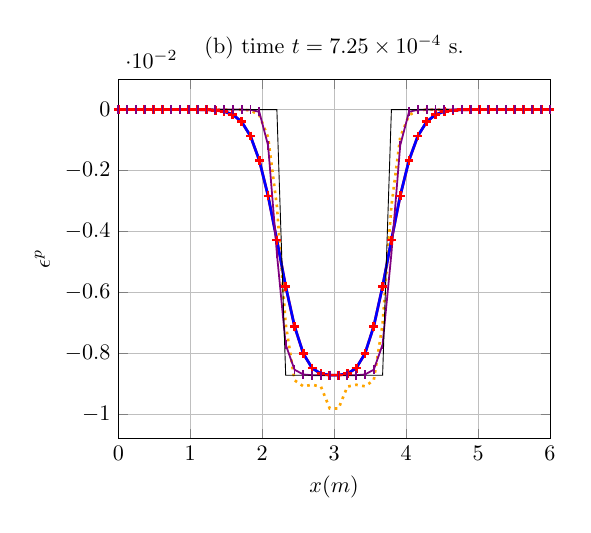
\begin{tikzpicture}[scale=0.8]
\begin{axis}[xlabel=$x (m)$,ylabel=$\epsilon^p$,ymajorgrids=true,xmajorgrids=true,legend pos=outer north east,title={(b) time $t = 7.25\times 10^{-4} $ s.},xmin=0.,xmax=6.]
\addplot[Red,very thick,mark=+,solid] coordinates {(0.0,-5.676632835751488e-19) (0.12244897959183673,-2.3898624238513766e-16) (0.24489795918367346,-3.735990751357306e-14) (0.36734693877551017,-2.3089144911084856e-12) (0.4897959183673469,-7.596762237094698e-11) (0.6122448979591837,-1.5415975357804979e-09) (0.7346938775510203,-1.0275730242331822e-08) (0.8571428571428571,-5.981932516353471e-08) (0.9795918367346939,-3.055798037968931e-07) (1.1020408163265305,-1.3747043608148892e-06) (1.2244897959183674,-5.4602719905226e-06) (1.346938775510204,-1.91823238251513e-05) (1.4693877551020407,-5.966726802674588e-05) (1.5918367346938775,-0.000164418651493838) (1.7142857142857142,-0.00040143744754996674) (1.836734693877551,-0.000868463225449077) (1.9591836734693877,-0.001665203797267752) (2.0816326530612246,-0.002832906100451628) (2.204081632653061,-0.004287995453610066) (2.326530612244898,-0.0058084443808726115) (2.4489795918367347,-0.007115753990208403) (2.571428571428571,-0.008016433919475449) (2.693877551020408,-0.008494471552590508) (2.816326530612245,-0.008677965053198252) (2.9387755102040813,-0.008723301560471332) (3.061224489795918,-0.008723301560471332) (3.183673469387755,-0.008677965053198252) (3.306122448979592,-0.00849447155259052) (3.4285714285714284,-0.008016433919475457) (3.5510204081632653,-0.007115753990208413) (3.673469387755102,-0.005808444380872623) (3.7959183673469385,-0.004287995453610076) (3.9183673469387754,-0.0028329061004516366) (4.040816326530612,-0.0016652037972677586) (4.163265306122449,-0.00086846322544908) (4.285714285714286,-0.0004014374475499613) (4.408163265306122,-0.00016441865149382611) (4.530612244897959,-5.9667268026732546e-05) (4.653061224489796,-1.918232382513086e-05) (4.775510204081632,-5.460271990507557e-06) (4.8979591836734695,-1.3747043608103478e-06) (5.020408163265306,-3.055798037929194e-07) (5.142857142857142,-5.981932515587126e-08) (5.26530612244898,-1.027573023324921e-08) (5.387755102040816,-1.5415975312391917e-09) (5.5102040816326525,-7.596762123562041e-11) (5.63265306122449,-2.308913923445202e-12) (5.755102040816326,-3.7358772187005907e-14) (5.877551020408163,-2.4097306387765065e-16) (6.0,-8.514949253627233e-19) };
\addplot[Orange,very thick,mark=none,dotted] coordinates {(0.0011999999999999927,0.0) (0.12359999999999997,0.0) (0.24599999999999994,0.0) (0.36839999999999995,0.0) (0.4907999999999999,-2.7815500895182294e-17) (0.6131999999999999,-3.8601103283110115e-17) (0.7355999999999999,-9.252911522274926e-17) (0.858,-1.5806584131150017e-15) (0.9803999999999998,-5.879373777480353e-14) (1.1027999999999998,-1.8355798153650192e-12) (1.2251999999999996,-4.7669529631024315e-11) (1.3475999999999997,-1.0242256048179808e-09) (1.4699999999999998,-1.8058382315295082e-08) (1.5923999999999996,-2.5837987508717037e-07) (1.7147999999999997,-2.955811391515107e-06) (1.8371999999999995,-2.650197421873382e-05) (1.9595999999999996,-0.00018124424208182778) (2.0819999999999994,-0.0009100274220600003) (2.2043999999999997,-0.0031724216849822393) (2.3267999999999995,-0.007051694130212292) (2.4491999999999994,-0.00889183395524355) (2.5715999999999997,-0.009090350906665956) (2.6939999999999995,-0.009040490458691425) (2.8163999999999993,-0.009101543401127671) (2.9387999999999996,-0.009819714666194801) (3.0611999999999995,-0.0098197146661948) (3.1835999999999993,-0.009101543401127772) (3.305999999999999,-0.009040490458691437) (3.4283999999999994,-0.009090350906665936) (3.5507999999999993,-0.008891833955243515) (3.673199999999999,-0.007051694130212307) (3.7955999999999994,-0.00317242168498228) (3.9179999999999993,-0.0009100274220600108) (4.040399999999999,-0.0001812442420818062) (4.1628,-2.6501974218710267e-05) (4.2852,-2.955811391528448e-06) (4.4076,-2.5837987506361237e-07) (4.53,-1.805838232863517e-08) (4.6524,-1.0242256082239605e-09) (4.7748,-4.766954637709118e-11) (4.8972,-1.835552283695766e-12) (5.0196,-5.885107176644462e-14) (5.142,-1.5667506626674108e-15) (5.2644,-6.897108895438059e-17) (5.3868,-1.7029898507254465e-18) (5.5092,-1.5043077014741444e-17) (5.6316,-1.7029898507254465e-18) (5.754,-1.4759245372953867e-17) (5.8764,-1.7029898507254465e-18) (5.9988,0.0) };
\addplot[Blue,very thick,mark=none,solid] coordinates {(0.0011999999999999927,0.0) (0.12359999999999997,-2.384185791015625e-16) (0.24599999999999994,-3.736019134521484e-14) (0.36839999999999995,-2.3089170455932617e-12) (0.4907999999999999,-7.596761584281921e-11) (0.6131999999999999,-1.5415975272655486e-09) (0.7355999999999999,-1.0275730234384537e-08) (0.858,-5.981932516098023e-08) (0.9803999999999998,-3.055798037946224e-07) (1.1027999999999998,-1.374704360806942e-06) (1.2251999999999996,-5.4602719905078414e-06) (1.3475999999999997,-1.9182323825132847e-05) (1.4699999999999998,-5.96672680267334e-05) (1.5923999999999996,-0.00016441865149382948) (1.7147999999999997,-0.000401437447549963) (1.8371999999999995,-0.0008684632254490853) (1.9595999999999996,-0.0016652037972677588) (2.0819999999999994,-0.002832906100451636) (2.2043999999999997,-0.00428799545361008) (2.3267999999999995,-0.005808444380872625) (2.4491999999999994,-0.007115753990208417) (2.5715999999999997,-0.00801643391947546) (2.6939999999999995,-0.008494471552590525) (2.8163999999999993,-0.00867796505319826) (2.9387999999999996,-0.008723301560471344) (3.0611999999999995,-0.008723301560471344) (3.1835999999999993,-0.00867796505319826) (3.305999999999999,-0.008494471552590525) (3.4283999999999994,-0.00801643391947546) (3.5507999999999993,-0.007115753990208417) (3.673199999999999,-0.005808444380872625) (3.7955999999999994,-0.00428799545361008) (3.9179999999999993,-0.002832906100451636) (4.040399999999999,-0.0016652037972677588) (4.1628,-0.0008684632254490853) (4.2852,-0.000401437447549963) (4.4076,-0.00016441865149382948) (4.53,-5.96672680267334e-05) (4.6524,-1.9182323825132847e-05) (4.7748,-5.4602719905078414e-06) (4.8972,-1.374704360806942e-06) (5.0196,-3.055798037946224e-07) (5.142,-5.981932516098023e-08) (5.2644,-1.0275730234384537e-08) (5.3868,-1.5415975272655486e-09) (5.5092,-7.596761584281921e-11) (5.6316,-2.3089170455932617e-12) (5.754,-3.736019134521484e-14) (5.8764,-2.384185791015625e-16) (5.9988,0.0) };
\addplot[Purple,thick,mark=|,solid] coordinates {(0.0011999999999999927,0.0) (0.12359999999999997,0.0) (0.24599999999999994,0.0) (0.36839999999999995,0.0) (0.4907999999999999,0.0) (0.6131999999999999,0.0) (0.7355999999999999,0.0) (0.858,-2.9802322387695314e-17) (0.9803999999999998,-1.329183578491211e-15) (1.1027999999999998,-4.1437149047851564e-14) (1.2251999999999996,-1.151418685913086e-12) (1.3475999999999997,-2.871338725090027e-11) (1.4699999999999998,-6.46675306558609e-10) (1.5923999999999996,-1.3273197644948959e-08) (1.7147999999999997,-2.510719147503376e-07) (1.8371999999999995,-4.397006492173672e-06) (1.9595999999999996,-7.414553616920114e-05) (2.0819999999999994,-0.0011776022671892642) (2.2043999999999997,-0.004734751896724993) (2.3267999999999995,-0.0077210124059583244) (2.4491999999999994,-0.008545394180645174) (2.5715999999999997,-0.008702161566804558) (2.6939999999999995,-0.008725895690329093) (2.8163999999999993,-0.008728522360980612) (2.9387999999999996,-0.008728709209868348) (3.0611999999999995,-0.008728709209868348) (3.1835999999999993,-0.008728522360980612) (3.305999999999999,-0.008725895690329093) (3.4283999999999994,-0.008702161566804558) (3.5507999999999993,-0.008545394180645174) (3.673199999999999,-0.0077210124059583244) (3.7955999999999994,-0.004734751896724993) (3.9179999999999993,-0.0011776022671892642) (4.040399999999999,-7.414553616920114e-05) (4.1628,-4.397006492173672e-06) (4.2852,-2.510719147562981e-07) (4.4076,-1.3273197644948959e-08) (4.53,-6.466753005981446e-10) (4.6524,-2.8713399171829228e-11) (4.7748,-1.1514246463775635e-12) (4.8972,-4.1437149047851564e-14) (5.0196,-1.329183578491211e-15) (5.142,-2.9802322387695314e-17) (5.2644,0.0) (5.3868,0.0) (5.5092,0.0) (5.6316,0.0) (5.754,0.0) (5.8764,0.0) (5.9988,0.0) };
\addplot[black,thin,mark=none,solid] coordinates {(0.0,-0.0) (0.12244897959183673,-0.0) (0.24489795918367346,-0.0) (0.36734693877551017,-0.0) (0.4897959183673469,-0.0) (0.6122448979591837,-0.0) (0.7346938775510203,-0.0) (0.8571428571428571,-0.0) (0.9795918367346939,-0.0) (1.1020408163265305,-0.0) (1.2244897959183674,-0.0) (1.346938775510204,-0.0) (1.4693877551020407,-0.0) (1.5918367346938775,-0.0) (1.7142857142857142,-0.0) (1.836734693877551,-0.0) (1.9591836734693877,-0.0) (2.0816326530612246,-0.0) (2.204081632653061,-0.0) (2.326530612244898,-0.008728715609439695) (2.4489795918367347,-0.008728715609439695) (2.571428571428571,-0.008728715609439695) (2.693877551020408,-0.008728715609439695) (2.816326530612245,-0.008728715609439695) (2.9387755102040813,-0.008728715609439695) (3.061224489795918,-0.008728715609439695) (3.183673469387755,-0.008728715609439695) (3.306122448979592,-0.008728715609439695) (3.4285714285714284,-0.008728715609439695) (3.5510204081632653,-0.008728715609439695) (3.673469387755102,-0.008728715609439695) (3.7959183673469385,-0.0) (3.9183673469387754,-0.0) (4.040816326530612,-0.0) (4.163265306122449,-0.0) (4.285714285714286,-0.0) (4.408163265306122,-0.0) (4.530612244897959,-0.0) (4.653061224489796,-0.0) (4.775510204081632,-0.0) (4.8979591836734695,-0.0) (5.020408163265306,-0.0) (5.142857142857142,-0.0) (5.26530612244898,-0.0) (5.387755102040816,-0.0) (5.5102040816326525,-0.0) (5.63265306122449,-0.0) (5.755102040816326,-0.0) (5.877551020408163,-0.0) (6.0,-0.0) };
%\legend{dgmpm,fem,fvm,fvm (SB),exact}
\end{axis}
\end{tikzpicture}
%%% Local Variables:
%%% mode: latex
%%% TeX-master: "../../mainManuscript"
%%% End:
}
  {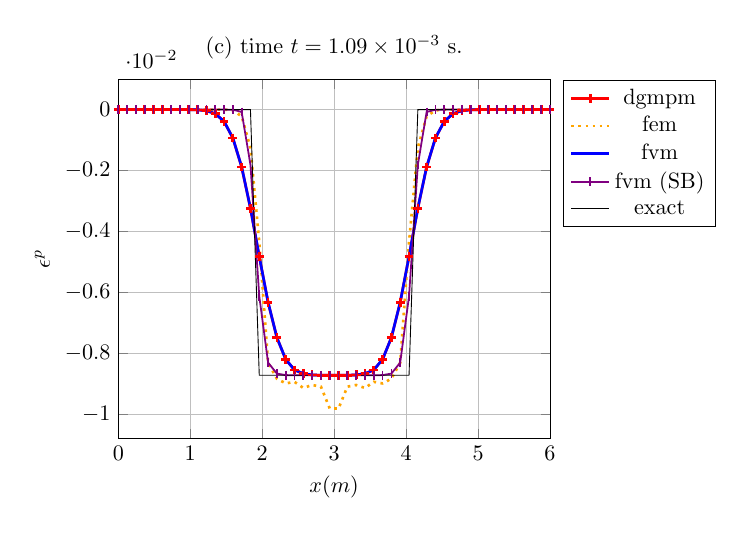
\begin{tikzpicture}[scale=0.8]
\begin{axis}[xlabel=$x (m)$,ylabel=$\epsilon^p$,ymajorgrids=true,xmajorgrids=true,legend pos=outer north east,title={(c) time $t = 1.09\times 10^{-3} $ s.},xmin=0.,xmax=6.]
\addplot[Red,very thick,mark=+,solid] coordinates {(0.0,-5.676632835751488e-19) (0.12244897959183673,-2.3898624238513766e-16) (0.24489795918367346,-3.735990751357306e-14) (0.36734693877551017,-2.3089144911084856e-12) (0.4897959183673469,-7.596762237094698e-11) (0.6122448979591837,-1.5415975357804979e-09) (0.7346938775510203,-2.1087029002110162e-08) (0.8571428571428571,-2.0628580472526095e-07) (0.9795918367346939,-1.5051975779320511e-06) (1.1020408163265305,-8.452232526292688e-06) (1.2244897959183674,-3.741900938747327e-05) (1.346938775510204,-0.00013315210803806102) (1.4693877551020407,-0.00038701776930482674) (1.5918367346938775,-0.0009319386970470464) (1.7142857142857142,-0.0018842066770200564) (1.836734693877551,-0.0032431409441831516) (1.9591836734693877,-0.004827293901207316) (2.0816326530612246,-0.00633202118341673) (2.204081632653061,-0.007489880430691718) (2.326530612244898,-0.008204526972019307) (2.4489795918367347,-0.008552921390073501) (2.571428571428571,-0.008674876019514461) (2.693877551020408,-0.008716486656783273) (2.816326530612245,-0.008726887116624966) (2.9387755102040813,-0.008728580772745199) (3.061224489795918,-0.008728580772745199) (3.183673469387755,-0.008726887116624966) (3.306122448979592,-0.00871648665678328) (3.4285714285714284,-0.008674876019514466) (3.5510204081632653,-0.008552921390073511) (3.673469387755102,-0.008204526972019318) (3.7959183673469385,-0.007489880430691721) (3.9183673469387754,-0.00633202118341673) (4.040816326530612,-0.0048272939012073204) (4.163265306122449,-0.0032431409441831525) (4.285714285714286,-0.001884206677020053) (4.408163265306122,-0.0009319386970470392) (4.530612244897959,-0.0003870177693048181) (4.653061224489796,-0.0001331521080380519) (4.775510204081632,-3.7419009387462476e-05) (4.8979591836734695,-8.452232526284741e-06) (5.020408163265306,-1.5051975779246716e-06) (5.142857142857142,-2.0628580471617835e-07) (5.26530612244898,-2.1087028991608393e-08) (5.387755102040816,-1.5415975312391917e-09) (5.5102040816326525,-7.596762123562041e-11) (5.63265306122449,-2.308913923445202e-12) (5.755102040816326,-3.7358772187005907e-14) (5.877551020408163,-2.4097306387765065e-16) (6.0,-8.514949253627233e-19) };
\addplot[Orange,very thick,mark=none,dotted] coordinates {(0.0011999999999999927,0.0) (0.12359999999999997,0.0) (0.24599999999999994,0.0) (0.36839999999999995,0.0) (0.4907999999999999,-2.7815500895182294e-17) (0.6131999999999999,-3.8601103283110115e-17) (0.7355999999999999,-2.0038513910202753e-16) (0.858,-1.7291875112624395e-14) (0.9803999999999998,-1.4890633878253755e-12) (1.1027999999999998,-8.711066870462328e-11) (1.2251999999999996,-3.5097774352346146e-09) (1.3475999999999997,-9.795044328882581e-08) (1.4699999999999998,-1.8896649221051307e-06) (1.5923999999999996,-2.4938869347233433e-05) (1.7147999999999997,-0.00022044973282056137) (1.8371999999999995,-0.0012586085323126788) (1.9595999999999996,-0.004366206064980092) (2.0819999999999994,-0.008315998828072487) (2.2043999999999997,-0.008841830788122323) (2.3267999999999995,-0.008995195469072521) (2.4491999999999994,-0.008944386605810638) (2.5715999999999997,-0.009146349400835571) (2.6939999999999995,-0.00904766889023616) (2.8163999999999993,-0.00910247337367582) (2.9387999999999996,-0.009819714666194801) (3.0611999999999995,-0.0098197146661948) (3.1835999999999993,-0.009102473373675955) (3.305999999999999,-0.009047668890236175) (3.4283999999999994,-0.009146349400835545) (3.5507999999999993,-0.008944386605810636) (3.673199999999999,-0.008995195469072475) (3.7955999999999994,-0.00884183078812235) (3.9179999999999993,-0.008315998828072471) (4.040399999999999,-0.004366206064980109) (4.1628,-0.0012586085323127117) (4.2852,-0.00022044973282050575) (4.4076,-2.4938869347250462e-05) (4.53,-1.8896649221051307e-06) (4.6524,-9.795044333225205e-08) (4.7748,-3.5097774522645135e-09) (4.8972,-8.711060172035581e-11) (5.0196,-1.4891476858229865e-12) (5.142,-1.7265194938296362e-14) (5.2644,-1.9045103163946243e-16) (5.3868,-1.7029898507254465e-18) (5.5092,-1.5043077014741444e-17) (5.6316,-1.7029898507254465e-18) (5.754,-1.4759245372953867e-17) (5.8764,-1.7029898507254465e-18) (5.9988,0.0) };
\addplot[Blue,very thick,mark=none,solid] coordinates {(0.0011999999999999927,0.0) (0.12359999999999997,-2.384185791015625e-16) (0.24599999999999994,-3.736019134521484e-14) (0.36839999999999995,-2.3089170455932617e-12) (0.4907999999999999,-7.596761584281921e-11) (0.6131999999999999,-1.5415975272655486e-09) (0.7355999999999999,-2.1087028992176057e-08) (0.858,-2.0628580471873284e-07) (0.9803999999999998,-1.5051975779294967e-06) (1.1027999999999998,-8.452232526284456e-06) (1.2251999999999996,-3.741900938746333e-05) (1.3475999999999997,-0.00013315210803804993) (1.4699999999999998,-0.00038701776930482386) (1.5923999999999996,-0.0009319386970470428) (1.7147999999999997,-0.001884206677020061) (1.8371999999999995,-0.003243140944183153) (1.9595999999999996,-0.004827293901207322) (2.0819999999999994,-0.006332021183416736) (2.2043999999999997,-0.007489880430691725) (2.3267999999999995,-0.008204526972019321) (2.4491999999999994,-0.008552921390073513) (2.5715999999999997,-0.008674876019514464) (2.6939999999999995,-0.008716486656783276) (2.8163999999999993,-0.008726887116624964) (2.9387999999999996,-0.008728580772745204) (3.0611999999999995,-0.008728580772745204) (3.1835999999999993,-0.008726887116624964) (3.305999999999999,-0.008716486656783276) (3.4283999999999994,-0.008674876019514464) (3.5507999999999993,-0.008552921390073513) (3.673199999999999,-0.008204526972019321) (3.7955999999999994,-0.007489880430691725) (3.9179999999999993,-0.006332021183416736) (4.040399999999999,-0.004827293901207322) (4.1628,-0.003243140944183153) (4.2852,-0.001884206677020061) (4.4076,-0.0009319386970470428) (4.53,-0.00038701776930482386) (4.6524,-0.00013315210803804993) (4.7748,-3.741900938746333e-05) (4.8972,-8.452232526284456e-06) (5.0196,-1.5051975779294967e-06) (5.142,-2.0628580471873284e-07) (5.2644,-2.1087028992176057e-08) (5.3868,-1.5415975272655486e-09) (5.5092,-7.596761584281921e-11) (5.6316,-2.3089170455932617e-12) (5.754,-3.736019134521484e-14) (5.8764,-2.384185791015625e-16) (5.9988,0.0) };
\addplot[Purple,thick,mark=|,solid] coordinates {(0.0011999999999999927,0.0) (0.12359999999999997,0.0) (0.24599999999999994,0.0) (0.36839999999999995,0.0) (0.4907999999999999,0.0) (0.6131999999999999,0.0) (0.7355999999999999,0.0) (0.858,-2.8014183044433593e-16) (0.9803999999999998,-2.1100044250488282e-14) (1.1027999999999998,-1.2365996837615966e-12) (1.2251999999999996,-5.9033864736557e-11) (1.3475999999999997,-2.3761736869812012e-09) (1.4699999999999998,-8.325840687155723e-08) (1.5923999999999996,-2.6323343349337577e-06) (1.7147999999999997,-7.853228000084162e-05) (1.8371999999999995,-0.0018212430710175336) (1.9595999999999996,-0.006137739318747551) (2.0819999999999994,-0.008311894308815801) (2.2043999999999997,-0.008672824985492957) (2.3267999999999995,-0.008722601697817814) (2.4491999999999994,-0.00872819127980076) (2.5715999999999997,-0.008728663911155045) (2.6939999999999995,-0.008728711882144921) (2.8163999999999993,-0.008728715435078365) (2.9387999999999996,-0.0087287156054703) (3.0611999999999995,-0.0087287156054703) (3.1835999999999993,-0.008728715435078365) (3.305999999999999,-0.008728711882144921) (3.4283999999999994,-0.008728663911155045) (3.5507999999999993,-0.00872819127980076) (3.673199999999999,-0.008722601697817814) (3.7955999999999994,-0.008672824985492957) (3.9179999999999993,-0.008311894308815794) (4.040399999999999,-0.006137739318747556) (4.1628,-0.0018212430710175217) (4.2852,-7.853228000084758e-05) (4.4076,-2.6323343349575996e-06) (4.53,-8.325840684175491e-08) (4.6524,-2.37617369890213e-09) (4.7748,-5.903387665748596e-11) (4.8972,-1.2365996837615966e-12) (5.0196,-2.1100044250488282e-14) (5.142,-2.8014183044433593e-16) (5.2644,0.0) (5.3868,0.0) (5.5092,0.0) (5.6316,0.0) (5.754,0.0) (5.8764,0.0) (5.9988,0.0) };
\addplot[black,thin,mark=none,solid] coordinates {(0.0,-0.0) (0.12244897959183673,-0.0) (0.24489795918367346,-0.0) (0.36734693877551017,-0.0) (0.4897959183673469,-0.0) (0.6122448979591837,-0.0) (0.7346938775510203,-0.0) (0.8571428571428571,-0.0) (0.9795918367346939,-0.0) (1.1020408163265305,-0.0) (1.2244897959183674,-0.0) (1.346938775510204,-0.0) (1.4693877551020407,-0.0) (1.5918367346938775,-0.0) (1.7142857142857142,-0.0) (1.836734693877551,-0.0) (1.9591836734693877,-0.008728715609439695) (2.0816326530612246,-0.008728715609439695) (2.204081632653061,-0.008728715609439695) (2.326530612244898,-0.008728715609439695) (2.4489795918367347,-0.008728715609439695) (2.571428571428571,-0.008728715609439695) (2.693877551020408,-0.008728715609439695) (2.816326530612245,-0.008728715609439695) (2.9387755102040813,-0.008728715609439695) (3.061224489795918,-0.008728715609439695) (3.183673469387755,-0.008728715609439695) (3.306122448979592,-0.008728715609439695) (3.4285714285714284,-0.008728715609439695) (3.5510204081632653,-0.008728715609439695) (3.673469387755102,-0.008728715609439695) (3.7959183673469385,-0.008728715609439695) (3.9183673469387754,-0.008728715609439695) (4.040816326530612,-0.008728715609439695) (4.163265306122449,-0.0) (4.285714285714286,-0.0) (4.408163265306122,-0.0) (4.530612244897959,-0.0) (4.653061224489796,-0.0) (4.775510204081632,-0.0) (4.8979591836734695,-0.0) (5.020408163265306,-0.0) (5.142857142857142,-0.0) (5.26530612244898,-0.0) (5.387755102040816,-0.0) (5.5102040816326525,-0.0) (5.63265306122449,-0.0) (5.755102040816326,-0.0) (5.877551020408163,-0.0) (6.0,-0.0) };
\legend{dgmpm,fem,fvm,fvm (SB),exact}
\end{axis}
\end{tikzpicture}
%%% Local Variables:
%%% mode: latex
%%% TeX-master: "../../mainManuscript"
%%% End:
}
  \caption{elastic-plastic RP epsp}
  \label{fig:epsp_elastoplastic_RP}
\end{figure}

\subsection{Two-dimensional elasticity}

\section{Hypoelastic solids}
Run again the test case with an updated CFL if many ppcs. Also look at the mass matrix that is probably zero for first node, the grid must be moved or something like that.
\section{Hyperelastic solids}
\subsection{One-dimensional problems}
\subsection{Two-dimensional problems}


%%% Local Variables:
%%% mode: latex
%%% TeX-master: "../mainManuscript"
%%% End:
